%%%%%%%%%%%%%%%%%%%%%%%%%%%%%%%%%%%%%%%%%%%%%%%%%%%%%%%%%%%%%%%%%%%%%%%%%%%%%%%%%%%%%%%%%
% 
% Document class for MEEC@DEE@ISEP dissertations, by Vitor M. R. Cunha - v1.3, Jul 2021
% Suggestions and comments are welcomed (vrc at isep dot ipp dot pt).
%
% Template provided as is, NO SUPPORT will be given.
% NO questions related to LaTeX will be answered, go to
% https://ftp.eq.uc.pt/software/TeX/info/lshort/english/lshort.pdf, or search the web.
%
% The DEE document class uses the LaTeX book base class, the original work credits are
% in the document class file.
%
% Overleaf template direct link:
% https://www.overleaf.com/latex/templates/isep-meec-msc-thesis-slash-dissertation-latex-template/zdyypsqypqnm
% or go to https://www.overleaf.com/gallery/, and search for: ISEP MEEC
%
%%%%%%%%%%%%%%%%%%%%%%%%%%%%%%%%%% MAIN SETTINGS %%%%%%%%%%%%%%%%%%%%%%%%%%%%%%%%%%%%%%%%

\documentclass[
MEECAS,			% Use this option to select your DEE degree, options: MEECAS, MEECSA, MEECPI, MEECTE
portuguese,		% Select document language, options: portuguese or english
%draft,			% Uncomment for draft mode (no pictures, no links, overfull hboxes) 
]{DEEclass}

% Use the 'preamble.tex' file (root folder) do add packages and macros. Keep your main.tex file clean.

% FYI, the following packages are preloaded with the document class:
% longtable, xcolor, graphicx, booktabs, caption, csquotes, hyperref,
% calc, listings, datetime2, siunitx, geometry, enumitem

%%%%%%%%%%%%%%%%%%%%%%%%%%%%%%%%%%%%%%%%%%%%%%%%%%%%%%%%%% extra packages
\usepackage{amsmath}		% the main package in the AMS-LATEX distribution
\usepackage{amsfonts}		% extended set of fonts for use in mathematics
\usepackage{amssymb}		% adds new symbols to be used in math mode
\usepackage{mathrsfs}		% math fonts, e.g., Laplace
\usepackage{float}			% provides the H float modifier option
\usepackage{multirow}		% tables \multirow command
\usepackage{subcaption}		% enables subfigures
\usepackage{lscape}			% for landscape mode
\usepackage{verbatim}		% new verbatim environment, \begin{comment}...\end{comment}, \verbatiminput
%\usepackage{pgfgantt}		% for Gantt charts, see https://ctan.org/pkg/pgfgantt

%add extra packages if needed here
%\usepackage[super]{nth}
%\usepackage{ordinalpt}
%\usepackage{fmtcount} % equivalent to \usepackage[super]{nth}
\usepackage[level]{fmtcount} % equivalent to \usepackage{nth}
\usepackage{siunitx}
\usepackage{pdfpages}
\usepackage{lineno}

%\newcommand{\ordinal}[1]{\ordinalnum{#1}\textsuperscript{o}}

\usepackage[normalem]{ulem}

\usepackage{url}
\def\UrlBreaks{\do\/\do-}
\usepackage{breakurl}

%%%%%%%%%%%%%%%%%%%%%%%%%%%%%%%%%%%%%%%%%%%%%%%%%%%%%%%%%% temp packages
\usepackage{lipsum}						% for fake text
%\usepackage[textsize=tiny]{todonotes}   % enable To-do notes, use the option "disable" to hide all notes, usage \todo{}

%\usepackage{draftwatermark}			% prints a watermark overlay, uncomment if needed
%\SetWatermarkText{**DRAFT**}
%\SetWatermarkScale{1}
%\SetWatermarkColor[gray]{0.8}

%%%%%%%%%%%%%%%%%%%%%%%%%%%%%%%%%%%%%%%%%%%%%%%%%%%%%%%%%% settings
\AtBeginDocument{					% Rendered PDF metadata:
\hypersetup{pdftitle=\ttitle} 		% Sets the PDF title to your dissertation title
\hypersetup{pdfauthor=\authorname} 	% Sets the PDF author to your name
}

%%%%%%%%%%%%%%%%%%%%%%%%%%%%%%%%%%%%%%%%%%%%%%%%%%%%%%%%%% user macros

%....










%%%%%%%%%%%%%%%%%%%%%%%%%%%%% DISSERTATION INFORMATION %%%%%%%%%%%%%%%%%%%%%%%%%%%%%%%%%%

\thesistitle{LaRE - Laboratório Remoto Expansível} % Your dissertation title

%\subdate{Janeiro, 2021} % Uncomment for a static submission date, or leave it as a comment for automatic date 

\author{Eduardo Manuel Martins Ramalhadeiro}	% Your name
\studentnumber{1210171}	% Your student number
\studentemail{1210171@isep.ipp.pt}	% Your student email address  

\advisor{André Vaz Fidalgo}{anf@isep.ipp.pt}	% Your advisor's name and email
%\coadvisor{Nome do Coorientador}{xxx@isep.ipp.pt}	% Your co-advisor's name and email, comment this line if not needed
%\company{Nome da Empresa, Lda.}	% The company name where you developed your work, comment this line if not needed
%\supervisor{Nome do Orientador da Empresa}{xxx@emailaddress.com}	% Your supervisor's name, comment this line if not needed

%%%%%%%%%%%%%%%%%%%%%%%%%%%%% USER DEFINED LISTS %%%%%%%%%%%%%%%%%%%%%%%%%%%%%%%%%%%%%%%%
\makeglossaries						% Consider the following files in the 'front' folder:
%----------------------------------------------------------------------------------------
%	GLOSSARY
%----------------------------------------------------------------------------------------

% Only the used entries will be displayed in the printed list, ie, you need to used a term at least once
% In italic if not in the main document language

% terms definition usage:
% \newglossaryentry{<tag>}{name={<term>},description={<description of the term>}}

\newglossaryentry{w3c}{
    name=W3C,
    description={O \acrfull{W3c} é uma organização internacional que desenvolve padrões e diretrizes para a \textit{web} visando garantir que a esta permaneça aberta, acessível e interoperável para todos. Os principais objetivos são promover a compatibilidade entre diferentes sistemas e garantir que a \textit{web} seja acessível a todos os utilizadores, independentemente das suas capacidades ou dispositivos. O \acrshort{W3c} trabalha em várias áreas, incluindo \acrshort{html} e \acrshort{css} \cite{W3C}.}
}

\newglossaryentry{sbc}{
    name=SBC,
    description={SBC ou \textit{Single-Board Computer} é um computador completo integrado numa única placa de circuito impresso, que inclui processador, memória, \textit{interfaces} de entrada/saída e, muitas vezes, conectividade de rede. Os SBC, como o \textit{Raspberry Pi}, são amplamente utilizados em aplicações de ensino, automação, prototipagem e sistemas embarcados, devido ao seu baixo custo, tamanho reduzido e versatilidade.}
}

\newglossaryentry{eeprom}{
    name=EEPROM,
    description={EEPROM (\textit{Electrically Erasable Programmable Read-Only Memory}) é um tipo de memória não volátil que pode ser escrita e apagada electricamente. É utilizada para armazenar pequenas quantidades de dados que devem ser preservados mesmo após desligar o sistema, como configurações, identificadores de \textit{hardware} ou parâmetros de funcionamento.}
}

\newglossaryentry{hat}{
    name=HAT,
    description={O termo HAT (\textit{Hardware Attached on Top}) refere-se a placas de expansão desenvolvidas segundo um padrão específico para o \textit{Raspberry Pi}. Estas placas ligam-se diretamente ao \textit{header GPIO} e incluem uma \textit{EEPROM} que permite ao sistema detectar automaticamente o acessório e configurar os respectivos pinos e \textit{interfaces} de forma transparente.}
}

\newglossaryentry{kicad}{
    name=KiCad,
    description={O \textit{KiCad} é um conjunto de ferramentas de \textit{software} de código aberto dedicada à Automatização do \textit{design} electrónico (EDA - \textit{Electronic Design Automation}). Esta ferramenta integra funcionalidades para a captura de esquemas elétricos e o desenho de placas de circuito impresso (\acrfull{pcb}), permitindo a exportação dos projetos nos formatos \textit{Gerber} e \textit{IPC-2581}. O \textit{KiCad} é compatível com os sistemas operativos \textit{Windows}, \textit{Linux} e \textit{MacOS}, sendo distribuída sob a licença GNU General Public License, versão 3 (GPL v3)}
}


\newglossaryentry{python}{
    name=Python,
    description={O \textit{Python} é uma linguagem de programação de alto nível, orientada a objecto, ou seja, com sintaxe mais simplificada e próxima da linguagem humana. É utilizada em \textit{web} ou servidores. Tem uma biblioteca padrão bastante completa e uma enorme comunidade que desenvolve ferramentas e bibliotecas (\textit{frameworks}) adicionais. O código é aberto e gratuito \cite{ThePython}. O \textit{Python} usa a indentação para delimitar blocos de código. Como curiosidade esta linguagem foi baptizada com este nome pelo seu criador, Guido van Rossum, como referência aos \textit{Monty Python}.}
}

\newglossaryentry{PIP}{
    name=pip,
    description={O \acrfull{pip} é o instalador de pacotes para Python que é usado para instalar pacotes dos repositórios Python e outros repositórios.}
}

\newglossaryentry{API}{
    name=API,
    description={Uma \acrfull{API} é um conjunto de definições e protocolos que permite que diferentes softwares se comuniquem entre si. No contexto de programação, uma \acrshort{API} fornece uma \textit{interface} através da qual se pode interagir com uma aplicação, biblioteca, ou serviço, utilizando comandos, funções, ou rotinas específicas.
        }}

\newglossaryentry{RaspberryPI}{
    name=Raspberry Pi,
    description={Raspberry Pi é uma gama de pequenos computadores acessíveis e versáteis que podem ser utilizados para vários projectos e fins, desenvolvidos pela \textit{Raspberry Pi Foundation}, uma organização educacional no Reino Unido. Esses dispositivos foram projetados para promover o ensino de ciências da computação básicas em escolas e países em desenvolvimento, além de serem populares entre entusiastas de eletrónica e \textit{makers} devido à sua versatilidade e custo acessível. Desde o seu lançamento, os modelos de RaspberryPI evoluíram significativamente, oferecendo maiores capacidades de processamento, memória e conectividade, adequados a uma ampla gama de aplicações, desde simples projetos de bricolagem a sistemas embebidos complexos e até mesmo servidores de baixo custo\cite{pifoundation}\cite{Raspberrypi}.
        }
}

\newglossaryentry{ESP32}{
    name=ESP32,
    description={O \textit{ESP32} é um microcontrolador de baixo custo e baixa potência com suporte para rede sem fios e \textit{Bluetooth}, desenvolvido pela \textit{Espressif Systems}. É amplamente utilizado em projetos de \acrshort{iot} devido às suas capacidades de conectividade e processamento.}
}

\newglossaryentry{arduino}{
    name=Arduino,
    description={O \textit{Arduino} é uma placa de desenvolvimento de código aberto baseada em \textit{hardware} e \textit{software} fáceis de utilizar. As placas \textit{Arduino} são capazes de ler entradas - luz num sensor, um dedo num botão ou uma mensagem do \textit{Twitter} - e transformá-las numa saída - activar um motor, ligar um \textit{LED}, publicar algo \textit{online} - utilizam a linguagem de programação \textit{Arduino} (baseada em \textit{Wiring}) e o \textit{software Arduino} (\acrshort{ide}), baseado em \textit{Processing} \cite{arduino}.
        }}

\newglossaryentry{industria40}{
    name=Industry 4.0,
    description={A Indústria 4.0, uma iniciativa da Alemanha, converteu-se num termo adoptado globalmente na última década. Dez anos após a introdução da Indústria 4.0, a Comissão Europeia anunciou a Indústria 5.0. Considera-se que a Indústria 4.0 é orientada para a tecnologia, enquanto a Indústria 5.0 é orientada para o valor \cite{industry4.0}.}
}

\newglossaryentry{triac}{
    name=TRIAC,
    description={O \acrfull{Triac} é um tiristor constituído por quatro camadas PNPN ou NPNP, com dois ânodos e uma porta. Contrariamente ao \acrshort{Scr}, o \acrshort{Triac} conduz nos dois sentidos da \acrshort{ca}, desde que se aplique à porta um impulso suficiente, positivo ou negativo. O \acrshort{Triac} é, geralmente, utilizado em \acrshort{ca}, no comando e controlo de potência} \cite{matias}.
}

\newglossaryentry{diac}{
    name=DIAC,
    description={O \acrfull{Diac} é um semicondutor que conduz a corrente elétrica num só sentido, tal como o díodo, mas de forma controlada, isto é, só após um disparo na sua porta. O \acrshort{Scr} é constituído por quatro camadas PNPN ou NPNP, tendo numa extremidade um ânodo e um cátodo e, ainda, a porta. Ao aplicar uma tensão positiva entre o ânodo e cátodo, ele conduz, desde que se aplique um impulso positivo na porta, com um determinado valor mínimo. Tanto o ânodo como a porta devem ser polarizados directamente, senão o \acrshort{Scr} não conduz} \cite{matias}.
}

\newglossaryentry{scr}{
    name=SCR,
    description={O \acrfull{Scr} é um semicondutor que conduz a corrente eléctrica nos dois sentidos, como se fossem dois díodos em paralelo e em sentidos contrários; isto é, ora funciona um díodo, durante a alternância positiva, ora funciona o outro na alternância negativa. A alimentação da porta do \acrshort{Triac} é, frequentemente, feita utilizando um \acrshort{Diac}} \cite{matias}.
}

\newglossaryentry{LABVIEW}{
    name=LabVIEW,
    description={O \textit{LabVIEW} é um ambiente de programação gráfica que proporciona aceleradores de produtividade únicos para o desenvolvimento de sistemas de teste, tais como uma abordagem intuitiva à programação, conetividade a qualquer instrumento e interfaces de utilizador totalmente integradas.}
}

%(Python Software Foundation, 2024; Beazley & Jones, 2013)

\newglossaryentry{pc/104}
{
    name=PC/104,
    description={As placas PC/104 são um padrão de computação embebida que se destaca pelo seu formato compacto e modula. Desenvolvidas pelo PC/104 \textit{Consortium}, estas placas são amplamente utilizadas em aplicações industriais e de controle, oferecendo uma combinação de robustez e flexibilidade.}
}

\newglossaryentry{JSON}
{
    name=JSON,
    description={\acrfull{json} é um formato leve para armazenamento e transporte de dados. É frequentemente utilizado na transmissão de informações entre um servidor e uma página \textit{web}, facilitando a comunicação entre diferentes sistemas. Além disso, o JSON é um formato auto-descritivo e de fácil compreensão, o que o torna amplamente adoptado no desenvolvimento de aplicações \textit{web} e na integração de \acrshort{api}s.}
}

\newglossaryentry{wrapper}{
    name=Wrapper,
    description={Um \textit{wrapper} em Python, neste contexto, refere-se a uma camada de código desenvolvida para encapsular e simplificar a utilização da \textit{interface} de programação do VirtualBench. Essencialmente, os \textit{wrappers} funcionam como intermediários que permitem aos programadores interagir com a funcionalidade subjacente do VirtualBench através de comandos Python mais simples e diretos. Isso facilita a automação de tarefas e a integração do VirtualBench com outros componentes ou \textit{scripts} desenvolvidos em \textit{Python}, proporcionando uma maneira mais eficiente e acessível de controlar e operar os dispositivos e funcionalidades oferecidos.}
}			% Edit to define your glossary entries list
%----------------------------------------------------------------------------------------
%	ACRONYMS LIST
%----------------------------------------------------------------------------------------

% Only the used entries will be displayed in the printed list, ie, you need to used a acronym at least once
% Full name in italic if not in the main document language

%acronym definition usage:
%\newacronym{<tag>}{<acronym>}{<full name>}

\newacronym{mb}{MB}{Megabyte}
\newacronym{lare}{LaRE}{Laboratório Remoto Expansível}
\newacronym{dee}{DEE}{Departamento de Engenharia Electrotécnica}
\newacronym{isep}{ISEP}{Instituto Superior de Engenharia do Porto}
\newacronym{meec}{MEEC}{Mestrado em Engenharia Electrotécnica e Computadores}
\newacronym{desi}{DESI}{Digital Economy and Society Index}
\newacronym{tic}{TIC}{Tecnologias da Informação e da Comunicação}
\newacronym{dn}{DN}{\textit{Diário de Notícias}}
\newacronym{ue}{ue}{União Europeia}
\newacronym{unesco}{UNESCO}{United Nations Educational, Scientific and Cultural Organization}
\newacronym{iot}{IoT}{Internet Of Things}
\newacronym{prr}{PRR}{Plano de Recuperação e Resiliência}
\newacronym{www}{WWW}{World Wide Web}
\newacronym{stem}{STEM}{Science, Technology, Engineering and Mathematics}
\newacronym{steam}{STE(A)M}{Science, Technology, Engineering, Arts and Mathematics}
\newacronym{ocde}{OCDE}{Organização para a Cooperação e Desenvolvimento Económico}
\newacronym{pisa}{PISA}{Program for International Student Assessment}
\newacronym{covid-19}{COVID-19}{SARS-CoV-2}
\newacronym{pafse}{PAFSE}{Partnerships for Science Education}
\newacronym{visir}{VISIR}{Virtual Instrument Systems in Reality}
\newacronym{spice}{SPICE}{Simulation Program for Integrated Circuits Emphasis}
\newacronym{pspice}{PSPICE}{Personal Computer Simulation Program for Integrated Circuits Emphasis}
\newacronym{pc}{PC}{\textit{Personal Computer}}
\newacronym{ca}{CA}{Corrente Alternada}
\newacronym{cc}{CC}{Corrente Contínua}
\newacronym{bth}{BTH}{Blekinge Institute of Technology}
\newacronym{ni}{NI}{\textit{National Instruments}}
\newacronym{eua}{EUA}{Estados Unidos da América}
\newacronym{ide}{IDE}{\textit{Integrated Development Environment}}
\newacronym{labview}{\textit{LabVIEW}}{\textit{Laboratory Virtual Instrument Engineering Workbench}}
\newacronym{microcontroladores}{$\mu$C}{\textit{microcontroladores}}
\newacronym{usb}{USB}{\textit{Universal Serial Bus}}
\newacronym{daq}{DAQ}{\textit{Data Acquisition}}
\newacronym{scada}{SCADA}{\textit{Supervisory Control and Data Acquisition}}
\newacronym{plc}{PLC}{\textit{Programmable Logic Controller}}
\newacronym{fpga}{FPGA}{\textit{Field Programmable Gate Array}}
\newacronym{arm}{ARM}{\textit{Advanced RISC Machine}}
\newacronym{mhsa}{MHSA}{\textit{Multipurpose Hardware and Software Architecture}}
\newacronym{matlab}{MATLAB}{\textit{MATrix LABoratory}}
\newacronym{ejs}{EJS}{\textit{Easy Java Simulations}}
\newacronym{diesel}{DIESEL}{\textit{Distance Internet-Based Embedded System Experimental Laboratory}}
\newacronym{laboratório remoto}{LR}{Laboratório Remoto}
\newacronym{ilab}{ISA}{\textit{iLab Shared Architecture}}
\newacronym{rlms}{RLMS}{\textit{Remote Laboratory Management System}}
\newacronym{mit}{MIT}{\textit{Massachusetts Institute of Technology}}
\newacronym{api}{API}{\textit{Application Programming Interface}}
\newacronym{lms}{LMS}{\textit{Learning Management System}}
\newacronym{puc}{PUC}{Pontifícia Universidade Católica}
\newacronym{mcr}{MCR}{Matriz de Comutação de Relés}
\newacronym{pic}{PIC}{\textit{Programmable Interrupt Controller}}
\newacronym{i2c}{\(I^2C\)}{\textit{Inter-Integrated Circuit}}
\newacronym{pxi}{PXI}{\textit{PCI eXtensions for Instrumentation}}
\newacronym{pilar}{PILAR}{\textit{Platform Integration of Laboratories based on the Architecture of visiR}}
\newacronym{sig}{SIG}{\textit{Special Interest Groups}}
\newacronym{Triac}{TRIAC}{\textit{Triode for Alternating Current}}
\newacronym{Diac}{DIAC}{(\textit{Diode for Alternating Current}}
\newacronym{Scr}{SCR}{\textit{Silicon Control Rectifier}}
\newacronym{lv}{LV}{Laboratório Virtual}
\newacronym{gpl}{GPL}{\textit{Gnu Public License}}
\newacronym{html}{HTML}{\textit{HyperText Markup Language}}
\newacronym{virtualbench}{VB}{\textit{VirtualBench}}
\newacronym{ram}{RAM}{\textit{Random Access Memory}}
\newacronym{spst}{SPST}{\textit{Single Pole Single Throw}}
\newacronym{dpst}{DPST}{\textit{Double Pole Single Throw}}
\newacronym{gpio}{GPIO}{\textit{General Purpose Input/Output}}
\newacronym{sipo}{SIPO}{\textit{Serial Input Parallel Output}}
\newacronym{css}{CSS}{\textit{Cascading Style Sheets}}
\newacronym{wsgi}{WSGI}{\textit{Web Server Gateway Interface}}
\newacronym{dom}{DOM}{\textit{Document Object Mode}}
\newacronym{ajax}{AJAX}{Asynchronous JavaScript e XML}
\newacronym{pip}{PIP}{\textit{Pip Installs Packages}}
\newacronym{http}{HTTP}{\textit{Hypertext Transfer Protocol}}
\newacronym{dmm}{DMM}{\textit{Digital Multimeter}}
\newacronym{url}{URL}{Uniform Resource Locator}
\newacronym{adc}{ADC}{\textit{Analog-to-Digital Converter}}
\newacronym{w3c}{W3C}{\textit{World Wide Web Consortium}}			% Edit to define your acronyms entries list
%----------------------------------------------------------------------------------------
%	SYMBOLS LIST
%----------------------------------------------------------------------------------------

% terms definition usage:
% \newglossaryentry{<tag>}{
% name={<symbol>},
% sort={<text for the alphabetical sorting>},
% description={<description of the symbol>},
% unit={<units to display>},
% type=symbolslist}

\newglossaryentry{i}{
name={\ensuremath{i}},
sort={i},
description={corrente},
unit=\si{\ampere},
type=symbolslist}

\newglossaryentry{v}{
name=\ensuremath{v},
sort={v},
description={tensão},
unit=\unit{\volt},
type=symbolslist}

\newglossaryentry{p}{
name=\ensuremath{P},
sort={p},
description={potência},
unit=\si{\watt},
type=symbolslist}

\newglossaryentry{r}{
name=\ensuremath{R},
sort={r},
description={resistência},
unit=\unit{\ohm},
type=symbolslist}

\newglossaryentry{omega}{
name=\ensuremath{\omega},
sort={z2},
description={velocidade angular},
unit=\si{\radian\per\second},
type=symbolslist}

\newglossaryentry{x}{
name=\ensuremath{x},
sort={x},
description={deslocamento},
unit=\si{\meter},
type=symbolslist}

% Greek: alpha,beta,gamma,delta,epsilon,zeta,eta,theta,iota,kappa,lambda,mu,nu,xi,omikron,pi,rho,sigma,tau,upsilon,phi,chi,psi,omega
				% Edit to define your symbols entries list

%%%%%%%%%%%%%%%%%%%%%%%%%%%%%%%%%%%%%%%%%%%%%%%%%%%%%%%%%%%%%%%%%%%%%%%%%%%%%%%%%%%%%%%%%
\begin{document}
\frontmatter

%----------------------------------------------------------------------------------------
%	TITLE PAGES
%----------------------------------------------------------------------------------------
\pagestyle{plain} % Default to the plain heading style until the thesis style is called for the body content
\printcoverpage
\printaftercoverpage
\cleardoublepage















%%%%%%%%%%%%%%%%%%%%%%%%%%%%%%%%%%% FRONTMATTER %%%%%%%%%%%%%%%%%%%%%%%%%%%%%%%%%%%%%%%%%
% Consider the following front matter sections provided as separate files in the 'front' folder.
% Comment the lines regarding the sections you will not use, or edit the file contents as needed

%----------------------------------------------------------------------------------------
%	DEDICATION
%----------------------------------------------------------------------------------------

\dedicatory{
Para ti, mãe

\vspace{1cm}

``(\ldots) às vezes ainda sou o menino

que adormeceu nos teus olhos''

\textit{Eugénio de Andrade}

} 
		% Edit if you want to dedicate your work to someone, or comment this line if not used
%----------------------------------------------------------------------------------------
%	ACKNOWLEDGEMENTS
%----------------------------------------------------------------------------------------

\begin{acknowledgements}
``A ordem dos factores é arbitrária'', portanto, os agradecimentos seguem sem uma ordem específica.

Um agradecimento muito especial terá de ser dirigido ao meu orientador - ``Oh Captain, my Captain'' - o Professor André Vaz Fidalgo. Obrigado pela (muita) paciência, liberdade, tolerância, sapiência, orientação e apoio durante todo o processo de desenvolvimento deste trabalho.

José Saramago escreveu o seguinte: ``\textit{Filho é um ser que nos emprestaram para um curso intensivo de como amar alguém além de nós mesmos, de como mudar nossos piores defeitos para darmos os melhores exemplos e de aprendermos a ter coragem. Isto mesmo! Ser pai ou mãe é o maior ato de coragem que alguém pode ter, porque é se expor a todo tipo de dor, principalmente da incerteza de estar agindo corretamente e do medo de perder algo tão amado. Perder? Como? Não é nosso, recordam-se? Foi apenas um empréstimo.}''

A decisão de avançar com esta dissertação surgiu com duas ideias em mente: adquirir mais conhecimento e (tentar) ser um exemplo e inspiração para a então única filha, Ana Ramalhadeiro, mostrando que, com esforço, dedicação e devoção, a glória acaba por chegar. E não esquecer: nunca é tarde demais para aprender. Pelo caminho nasceu a Maria Ramalhadeiro, que, por agora, só se interessa pela ``Patrulha Pata'' e os ``Mistérios dos Bichos'', mas cá estarei para, a seu tempo, lhe mostrar o exemplo e servir de inspiração.

À mãe mais linda do mundo — Elsa Mariana Lopes (e) Mota — obrigado pela paciência, apoio e compreensão durante todo este processo. Sem ti, nada disto seria possível, até porque estavas responsável pelo pagamento das propinas.

Ao meu pai e irmão, José e Eng.\textsuperscript{o} Rui Ramalhadeiro - \textit{a.k.a.} GNUUU - pelo incentivo; aos meus amigos, que não me ajudaram em nada, a não ser chatear para jantares e lanches.

Um agradecimento especial à Professora Cristina Sá pela ajuda na elaboração do documento, ao Professor Ernesto Martins e ao Eng.\textsuperscript{o} José Garcia pelos conselhos e esclarecimentos técnicos.

\end{acknowledgements}
	% Edit to add the due acknowledgements, or comment this line if not used
%----------------------------------------------------------------------------------------
%	ABSTRACT PAGES
%----------------------------------------------------------------------------------------

% IMPORTANT NOTE: the abstract must always be written in two languages. If the dissertation
% is written in Portuguese you have selected 'portuguese' as the language in the document class.
% Therefore, the portuguese version of the abstract must come first, so write it in the
% below area denoted by 'MAIN LANGUAGE ABSTRACT'. The english version follows in the
% 'SECOND LANGUAGE ABSTRACT' section.
% If the dissertation is written in English, first will come the abstract in English
% ('MAIN LANGUAGE ABSTRACT') and then in Portuguese ('SECOND LANGUAGE ABSTRACT').

\begin{abstract}
%%%%%%%%%%%%%%%%%%%%%%%%%%%%%% MAIN LANGUAGE ABSTRACT %%%%%%%%%%%%%%%%%%%%%%%%%%%%%%%%%%

A formação em engenharia, particularmente na área da electrónica, exige uma forte componente prática, frequentemente concretizada em contexto laboratorial. No entanto, os laboratórios físicos tradicionais apresentam desafios significativos, como custos elevados, exigência de espaço físico e limitação do acesso devido a restrições logísticas. Estes desafios foram agravados pelo surgimento da pandemia da \acrshort{covid-19}, em 2020. Perante estas limitações, os laboratórios remotos surgem como uma alternativa eficaz e promissora. Estes permitem que os estudantes realizem experiências reais em equipamentos físicos, através de controlo remoto, promovendo um acesso mais inclusivo, flexível e escalável ao ensino prático.

A presente dissertação descreve o processo de concepção de um laboratório remoto - \acrfull{lare} - para o ensino da electrónica, como alternativa viável ao \acrshort{visir}, com o compromisso adicional de ser um projecto \textit{open-source}, acessível a qualquer instituição de ensino, independentemente da sua localização geográfica. A matriz de placas, elemento central do sistema, foi desenvolvida com base numa arquitectura controlada por \textit{software}, sem dependência de plataformas proprietárias, garantindo assim que o sistema possa ser utilizado sem necessidade de licenças comerciais. Contudo, devido à actual falta de suporte da biblioteca \textit{pyVirtualBench} para sistemas \textit{Linux} e arquitecturas \acrfull{arm}, a implementação do \acrshort{lare} permanece, nesta fase, dependente de sistemas \textit{Windows} - um factor que limita a sua adopção em plataformas educativas mais versáteis e de baixo custo. No entanto, a arquitectura modular do \acrshort{lare} permite futuras expansões e adaptações a diferentes contextos pedagógicos.

Assim, este trabalho visa: contextualizar o papel dos laboratórios remotos no ensino; analisar alternativas existentes; identificar os requisitos técnicos (de \textit{hardware} e \textit{software}) para a construção de um laboratório remoto \textit{open-source} em conformidade com a licença \acrshort{gpl}; implementar e testar o \acrshort{lare}; e apresentar as suas vantagens, limitações e possíveis melhoramentos. A proposta assenta numa abordagem acessível e escalável, procurando contribuir para o reforço da aprendizagem prática e para a democratização do ensino experimental em engenharia.


%----------------------------------------------------------------------------------------

\vspace*{10mm} 
\noindent
\textbf{\keywordslabel}: laboratório remoto, ensino de electrónica, VirtualBench, controlo remoto, \textit{open-source}, acessibilidade, \acrshort{gpl}, \acrshort{lare}, \acrshort{visir}

%%%%%%%%%%%%%%%%%%%%%%%%% END OF THE MAIN LANGUAGE ABSTRACT %%%%%%%%%%%%%%%%%%%%%%%%%%%%%%
\end{abstract}
\begin{secondlangabstract}
%%%%%%%%%%%%%%%%%%%%%%%%%%%%%% SECOND LANGUAGE ABSTRACT %%%%%%%%%%%%%%%%%%%%%%%%%%%%%%%%%%

Engineering education, particularly in electronics, requires a strong practical component, typically delivered through hands-on laboratory work. However, traditional physical laboratories pose several challenges, including high operational costs, limited space, and restricted access due to logistical constraints. These issues were further intensified by the \acrshort{covid-19} pandemic in 2020. In response, remote laboratories have emerged as a promising and effective alternative, enabled by recent technological advances. These platforms allow students to perform real experiments on physical equipment via remote control, promoting more inclusive, flexible, and scalable access to practical learning.

This dissertation presents the development of a remote laboratory — the \acrfull{lare} — designed for electronics education. It aims to serve as an open-source, viable alternative to \acrshort{visir}, with universal accessibility regardless of the institution’s geographical location. The \acrshort{lare} system enables remote control of practical experiments and promotes equitable access to laboratory resources. The core component, a configurable board matrix, was developed using a software-controlled architecture that avoids proprietary dependencies, allowing use without commercial licenses. However, due to the current lack of support by the pyVirtualBench library for Linux systems and ARM architectures, the implementation of LARE remains, at this stage, dependent on Windows systems — a factor that limits its adoption on more versatile and low-cost educational platforms. Nevertheless, the modular architecture of \acrshort{lare} supports future extensions and adaptability to varied pedagogical contexts.

This work seeks to: contextualize the role of remote laboratories in education; review existing solutions; define the technical (hardware and software) requirements for building an open-source remote lab under the \acrshort{gpl} license; implement and test the \acrshort{lare}; and present its advantages, limitations, and possible improvements. The proposal aims to provide a scalable and accessible infrastructure that reinforces hands-on learning and democratizes experimental education in engineering.


%----------------------------------------------------------------------------------------

\vspace*{10mm} 
\noindent
\textbf{\keywordslabel}: remote laboratory, electronics education, VirtualBench, remote control, open-source, accessibility, \acrshort{gpl}, \acrshort{lare}, \acrshort{visir}.

%%%%%%%%%%%%%%%%%%%%%%%%%% END OF THE SECOND LANGUAGE ABSTRACT %%%%%%%%%%%%%%%%%%%%%%%%%%%%%
\end{secondlangabstract}

			% Edit the file to write the dissertation Abstract. Two languages are always required.
%----------------------------------------------------------------------------------------
%	FONTMATTER LISTS
%----------------------------------------------------------------------------------------
\pdfbookmark[0]{\contentsname}{toc}
\tableofcontents 	
\glsresetall
%----------------------------------------------------------------------------------------

% Of the following lists, comment the ones you will not use in your document

\listoffigures 			% Prints the list of figures

\listoftables 			% Prints the list of tables

\printlistoflistings	% Prints the list of listings (source code segments)

\printlistofterms		% Prints the list of USED terms (glossary)

\printlistofacronyms{XXXXXXXXI} % Prints the list of USED acronyms
% Change the argument with random letters to adjust the left alignment of the acronyms full name column

\printlistofsymbols		% Prints the list of ALL defined symbols
	% Edit the file to select the lists to be shown (figures, tables, source code segments, glossary, acronyms, symbols)

%%%%%%%%%%%%%%%%%%%%%%%%%%%%%%%%%%% MAINMATTER %%%%%%%%%%%%%%%%%%%%%%%%%%%%%%%%%%%%%%%%%
\mainmatter
\pagestyle{thesis}

% Include the chapters of the dissertation as separate files from the 'chapters' folder

%%%%%%%%%%%%%%%%%%%%%%%%%%%%%%%%%%%% Chapter Template

\chapter{Introdução} 	% Main chapter title
\label{Capítulo1} 		% For referencing the chapter elsewhere, usage \ref{Capítulo1}

\begin{flushright}
\textit{``So it begins''} \\[0.5em]
--- King Theoden, \textit{The Lord of the Rings: The Two Towers}
\end{flushright}
Esta dissertação insere-se no programa de Mestrado em Engenharia Eletrotécnica e de Computadores, Área de Especialização em Automação e Sistemas e tem como principal objectivo o desenvolvimento de um laboratório remoto aplicado ao ensino da electrónica.
Este capítulo aborda a motivação para a abordagem desta temática, nele é apresentada a contextualização, assim como os objectivos a serem atingidos e uma breve estruturação da dissertação.

\section{Enquadramento}
\label{sec: Enquadramento}
A educação em engenharia, especialmente em áreas como electrónica, depende fortemente de actividades prácticas. Os laboratórios são cruciais para que os estudantes possam aplicar os conceitos teóricos em cenários prácticos, desenvolver habilidades técnicas e enfrentar desafios reais \cite{Hofstein, BRINSON2015218}. No entanto, a manutenção e o acesso a laboratórios físicos tradicionais apresentam várias dificuldades, incluindo altos custos, limitações de espaço e a necessidade de supervisão constante por parte de instrutores ou professores qualificados \cite{feisel}. Além disso, o acesso a esses laboratórios pode ser restrito devido a factores como horários de funcionamento e a necessidade de presença física.

Nos últimos anos, os avanços na tecnologia, do \textit{eLearning} e na implementação da abordagem \acrfull{stem} abriram novas possibilidades para o ensino práctico da electrónica através de laboratórios remotos. Esses laboratórios permitem que os estudantes realizem experiências reais em equipamentos físicos controlados remotamente, independentemente da sua localização geográfica. A implementação de laboratórios remotos tem o potencial de democratizar o acesso ao ensino de qualidade, oferecendo oportunidades educacionais mais equitativas e inclusivas \cite{CORTER20112054}.

\section{Objectivos}
\label{sec:Objectivos}
A génese desta dissertação ocorreu há três anos e estava associada à ideia de desenvolver um \acrfull{lare} para o ensino da electrónica. Uma das soluções existentes no \acrfull{isep} é o \acrfull{visir}.
O \acrshort{visir} é um projecto - laboratório remoto (virtual) - que pode ser aplicado no vasto campo da engenharia electrotécnica e electrónica e na área da teoria e práctica de circuitos. Tem como objectivo definir, desenvolver e avaliar um conjunto de módulos educativos compostos por experiências práticas, virtuais e remotas \cite{visirisep}.
No entanto, o desenvolvimento deste laboratório remoto apresenta um grave problema, que corresponde ao facto de, por questões legais, não ser possível realizar qualquer tipo de modificação e/ou actualização ao \textit{firmware} da matriz que controla os relés. \textbf{\textcolor{red}{A REVER} - Prof.}

Partindo, então, destes pressupostos definiram-se os seguintes objectivos:
\begin{itemize}
    \item Contextualizar o uso dos laboratórios remotos no ensino;
    \item Estudar e analisar algumas das alternativas existentes, nomeadamente, o \acrshort{visir};
    \item Identificar os requisitos de \textit{hardware} e \textit{software} necessários para implementar o \acrshort{lare} como um projeto \textit{open-source}, em conformidade com a licença \acrfull{gpl}:
    \begin{itemize}
        \item Pesquisar, analisar e avaliar a implementação de um servidor;
        \item Pesquisar, analisar e avaliar as soluções de \textit{software} existentes para a integração do \acrfull{virtualbench} com o \acrshort{lare};
         \item Definir quais, e quantos, circuitos integrar;
    \end{itemize}
    \item Implementar e testar o \acrshort{lare};
    \item Identificar as vantagens e desvantagens do \acrshort{lare}, assim como possíveis melhoramentos;
    \item Apresentar resultados e conclusões da implementação do \acrshort{lare}.
\end{itemize}

\section{Estrutura do documento}
Esta dissertação está organizada em seis capítulos. Neste primeiro capítulo, foi feita uma breve introdução à implementação do \acrshort{lare} e aos objetivos que a orientam. O Capítulo~\ref{Capitulo2} aborda o estado da arte no que respeita à Educação Digital e à integração dos laboratórios no ensino. O Capítulo~\ref{Capítulo3} trata, de forma detalhada, os aspetos relacionados com o \acrshort{lare}, ao nível do \textit{hardware} e do \textit{software}. A implementação do \acrshort{lare} é apresentada no Capítulo~\ref{Capítulo4}. No Capítulo~\ref{Capítulo5} discutem-se os resultados, que servem de base para, no Capítulo~\ref{Capítulo6}, se apresentarem as conclusões e limitações da implementação do \acrshort{lare}.


%%%%%%%%%%%%%%%%%%%%%%%%%%%%%%%%%%%%

% Capítulo 2
\chapter{Estado da Arte}
\label{Capitulo2}

\begin{flushright}
\textit{``You are entering a world of pain.''} \\[0.5em]
--- Walter Sobchak, \textit{The Big Lebowski}
\end{flushright}
Tendo em conta a experiência do autor como professor numa escola secundária, neste capítulo procura-se fazer o enquadramento das principais dificuldades que a Educação (digital) atravessa em Portugal e discutir em que medida a integração da tecnologia digital na educação é essencial para criar ambientes de aprendizagem mais eficazes e adaptados à evolução do panorama digital. Explora-se o potencial de tecnologias, como os laboratórios remotos, para o desenvolvimento de experiências de aprendizagem personalizadas e reflete-se sobre a forma como podem ajudar a suprir estas mesmas dificuldades.
Face a isto, discute-se a ascensão do \textit{eLearning}, particularmente no contexto da abordagem \acrshort{stem}, assim como a evolução da educação das salas de aula tradicionais para ambientes virtuais, enfatizando as oportunidades e possibilidades de aprendizagem alargadas oferecidas pelo \textit{eLearning}

\section{Transformação digital na educação}
\label{sec:transformaçãodigital}
A educação está a sofrer grandes mudanças a nível tecnológico, social e humano. Estas foram impulsionadas pela \acrfull{covid-19}, que expôs as fragilidades em termos de gestão e capacitação dos recursos tecnológicos e do eLearning\footnote{Jay Cross, é conhecido por ter ``cunhado'' pela primeira vez o termo \textit{eLearning} \cite{jaycross}. Por isso, nesta dissertação, o termo será sempre referido desta forma, em vez de \textit{e-Learning}}. O sistema educativo português apresenta ainda várias fragilidades que ficaram particularmente evidentes nesse contexto. Ainda assim, graças a um grande esforço colectivo, foi possível responder de forma imediata a este enorme obstáculo. Num curto espaço de tempo, o ensino presencial e o contacto humano foram substituídos pelo ensino à distância. Estávamos pronto para isto?

Antes da pandemia, no Ensino Básico e Secundário, as tecnologias digitais eram mais frequentemente utilizadas como meio de comunicação do que como ferramenta pedagógica~\cite{oecd_using_2021}. Nas últimas duas décadas, Portugal já introduziu programas para abordar a digitalização na educação. O programa de digitalização contemplado no Plano de Ação para a Transição Digital (Resolução do Conselho de Ministros n.\textsuperscript{o} 30/2020, de 21 de abril) prevê, entre outras medidas, uma forte aposta na formação digital dos professores, no desenvolvimento digital das escolas e na disponibilização de recursos educativos digitais \cite{transicaodigital, capacitacaodigital}.

No mundo de hoje, cada vez mais digital, apesar de em 2024 o número de utilizadores da Internet se situar nos 5,5 mil milhões, ainda existem 2,6 mil milhões de pessoas sem acesso à Internet, como se pode observar no gráfico retirado do relatório ``\textit{ITU Facts \& Figures 2024}'' e apresentado na Figura~\ref{fig:numutilizadoresnet} \cite{broadbandcomission, itu2024facts}.

\begin{figure}[hbtp]
    \centering
    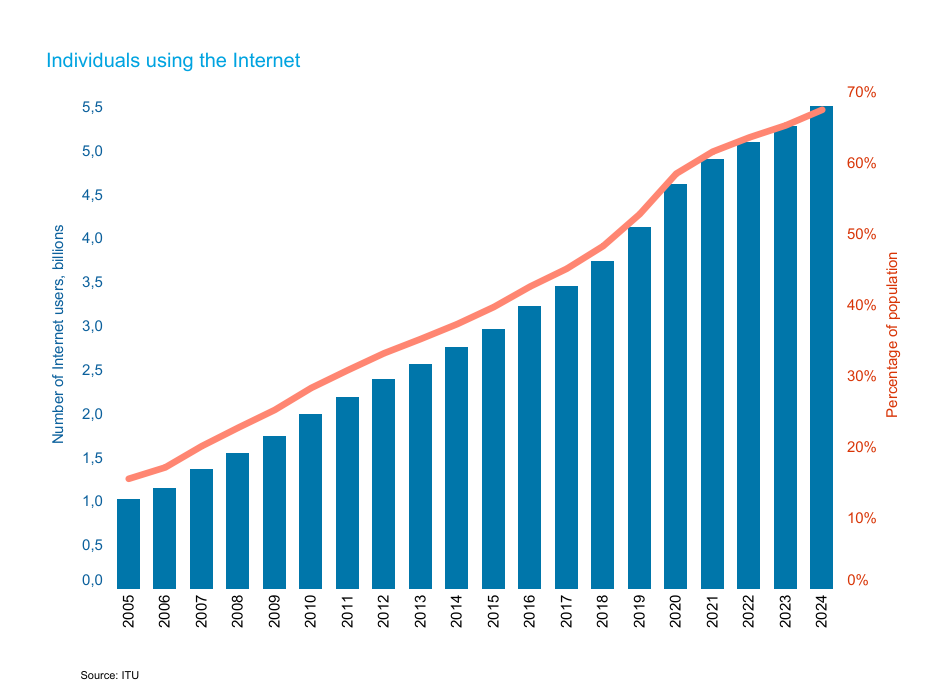
\includegraphics[width=0.65\textwidth]{figures/ITU-InternetUse.png}
    \caption{Número de utilizadores da Internet em todo o mundo, 2024 \cite{itu2024facts}}
    \label{fig:numutilizadoresnet}
\end{figure}
Este problema reduz o acesso a um mundo de informações disponíveis \textit{online} e limita o potencial de aprendizagem e crescimento, para não falar das competências digitais de que as pessoas necessitam para aprender e melhorar as suas vidas.
A crise da \acrshort{covid-19} demonstrou como a ligação à Internet é crucial para actividades quotidianas, como o trabalho e a aprendizagem. Hoje, mais do que nunca, é necessário reforçar as infraestruturas nacionais, de forma a garantir que a conectividade esteja amplamente disponível. É igualmente essencial reforçar os planos de conectividade das escolas e investir numa aprendizagem de qualidade, com o objectivo de melhorar o acesso à educação, os resultados da aprendizagem e o potencial de ganhos dos jovens, bem como o desenvolvimento socioeconómico das suas comunidades e países~\cite{TheDigitransf}.

Ainda que não constitua objectivo central desta dissertação proceder a uma análise exaustiva ao ``\textit{Digital Decade 2024 Country Report}'' \cite{DESI2024}, a consulta de alguns indicadores-chave permite constatar que, em 2023, Portugal registou uma taxa de 55,97\% da população com, pelo menos, competências digitais básicas - ligeiramente acima da média da União Europeia (55,56\%). Este progresso tem sido acompanhado por um crescimento sustentado no número de especialistas em \acrfull{tic}.
Contudo, o desempenho global de Portugal na dimensão Capital Humano, segundo o índice \acrfull{desi}, continua a posicionar-se abaixo da média europeia, como evidenciado no gráfico geral apresentado na Figura~\ref{fig:all_individuals}. A distribuição etária representada na Figura~\ref{fig:individuals} demonstra que Portugal se encontra entre os países com menor desempenho nas faixas etárias mais elevadas, revelando que persistem desafios significativos noutros indicadores que continuam a comprometer esta dimensão estratégica para a transição digital.

\begin{figure}[hbtp]
	\centering%
		\centering
		\subfloat[\centering Todos os individuos\label{fig:all_individuals}]{{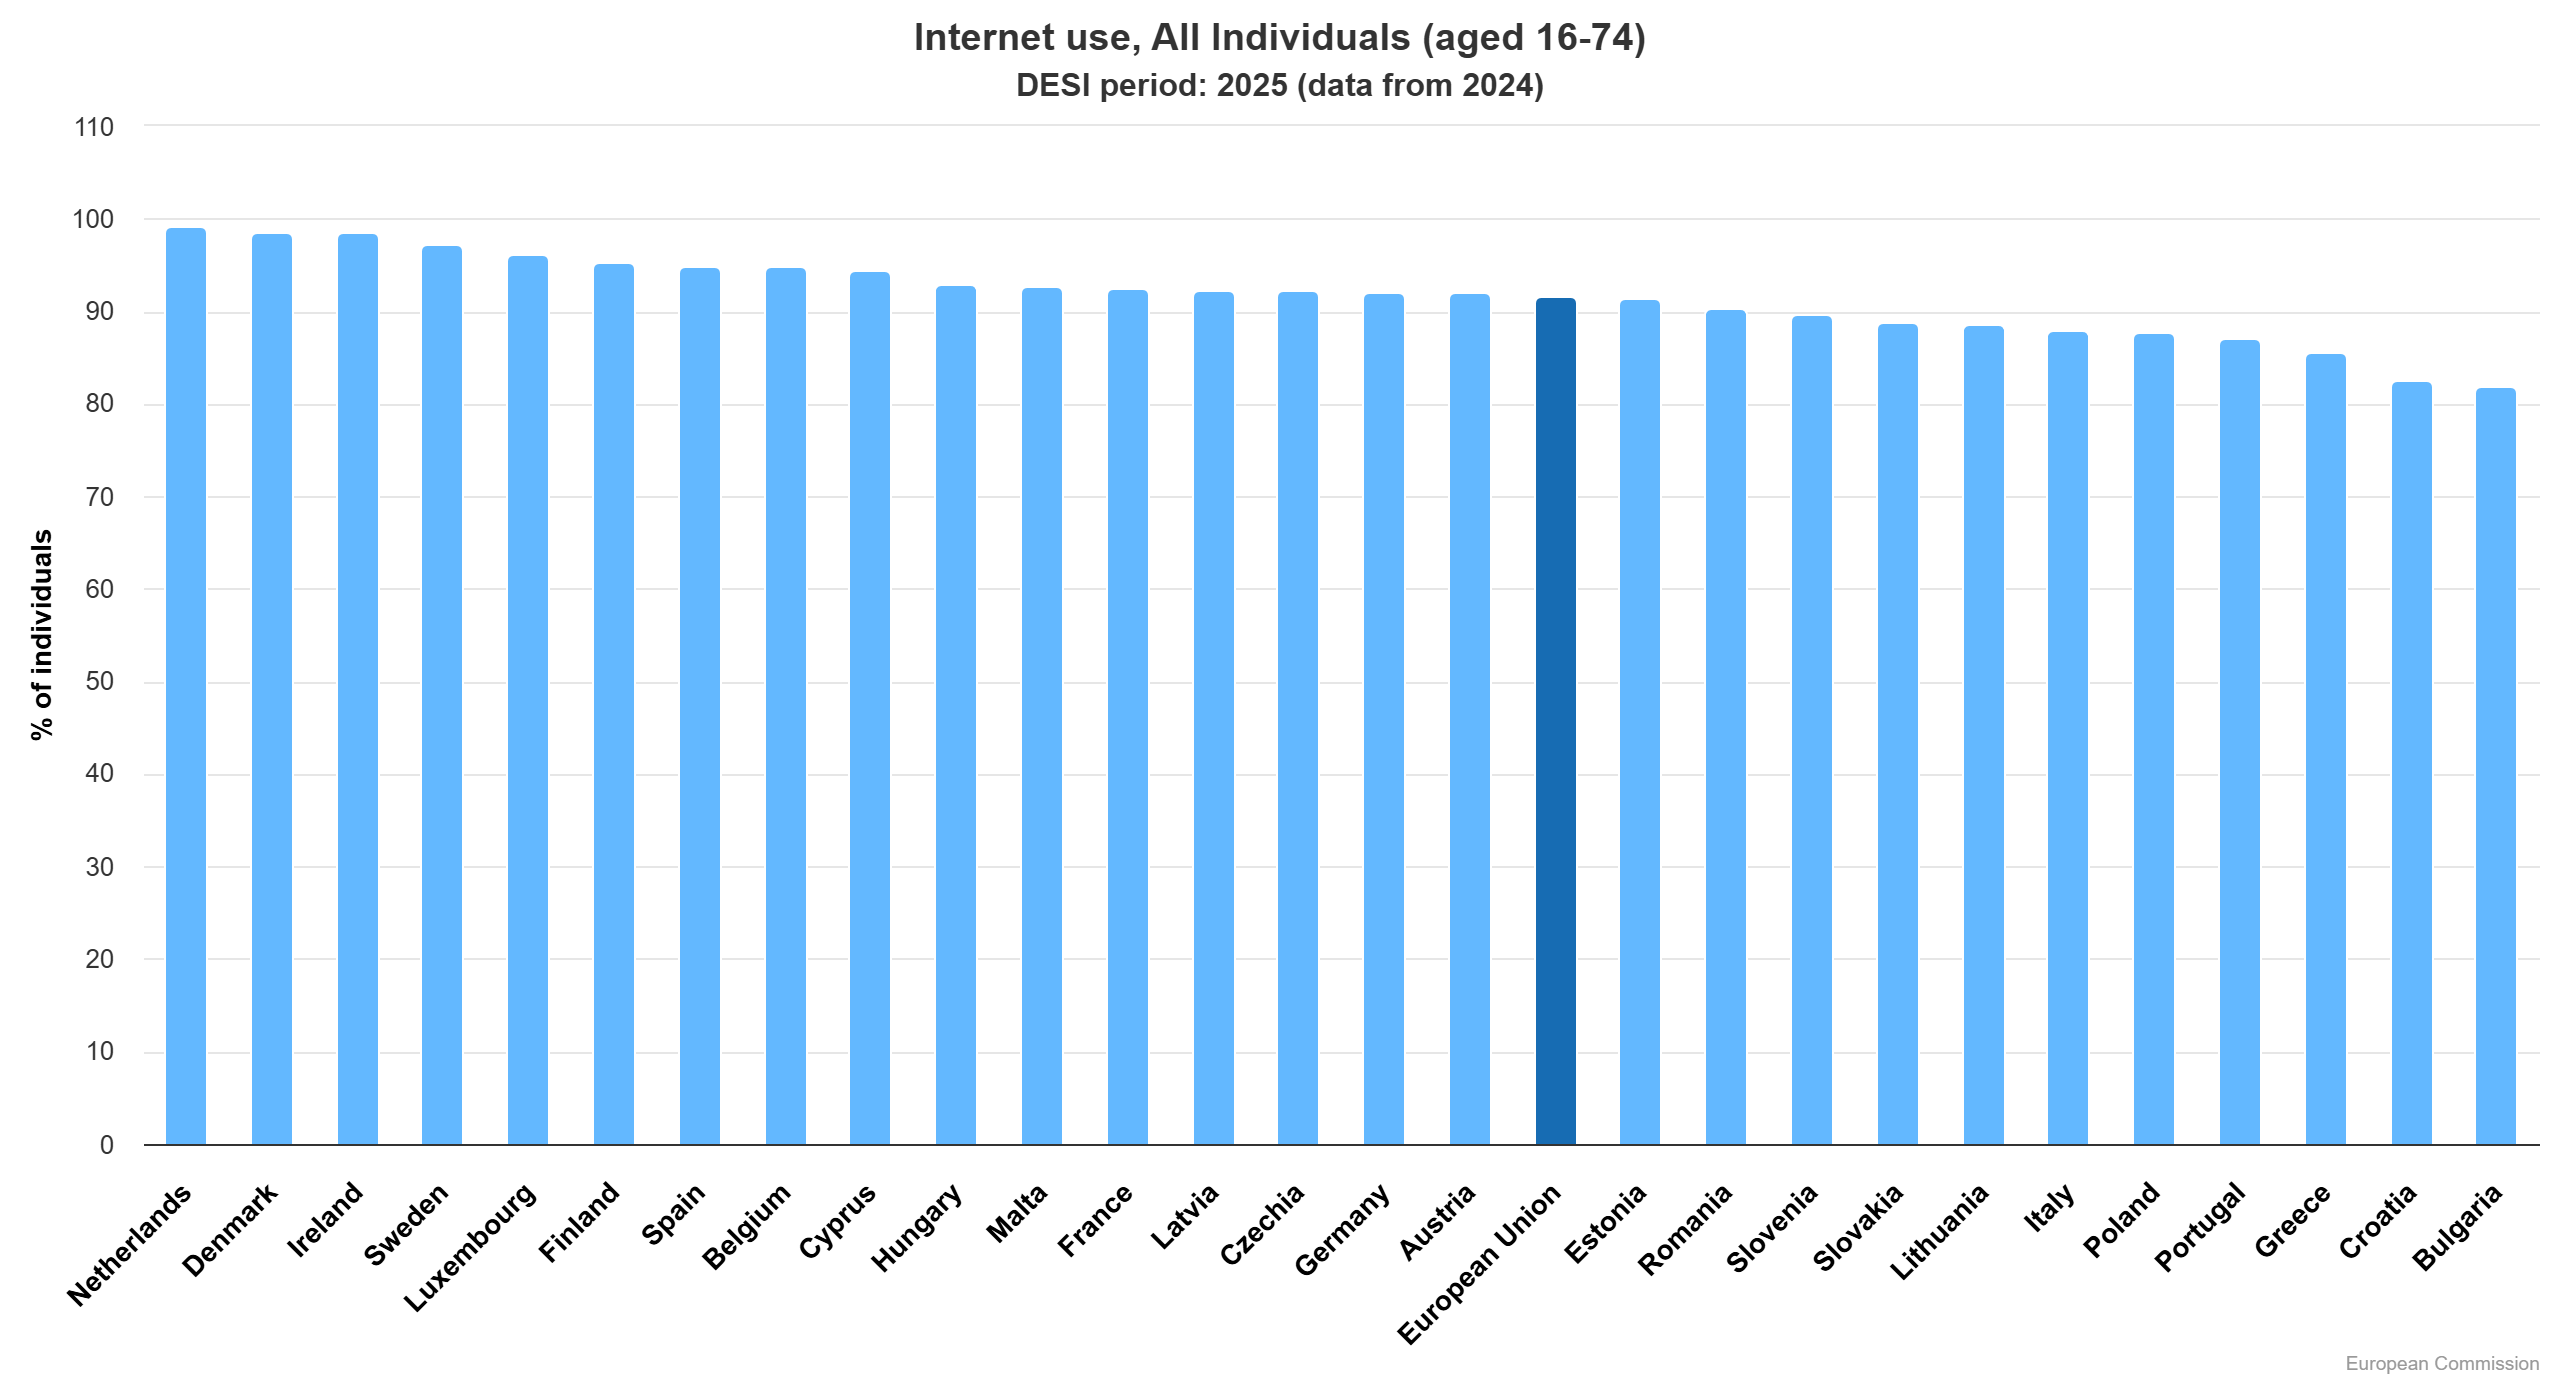
\includegraphics[width=6.3cm]{figures/internet-use-all-individ.png} }}%
		\qquad
		\subfloat[\centering Individuos entre 55 e 74 anos de idade\label{fig:individuals}]{{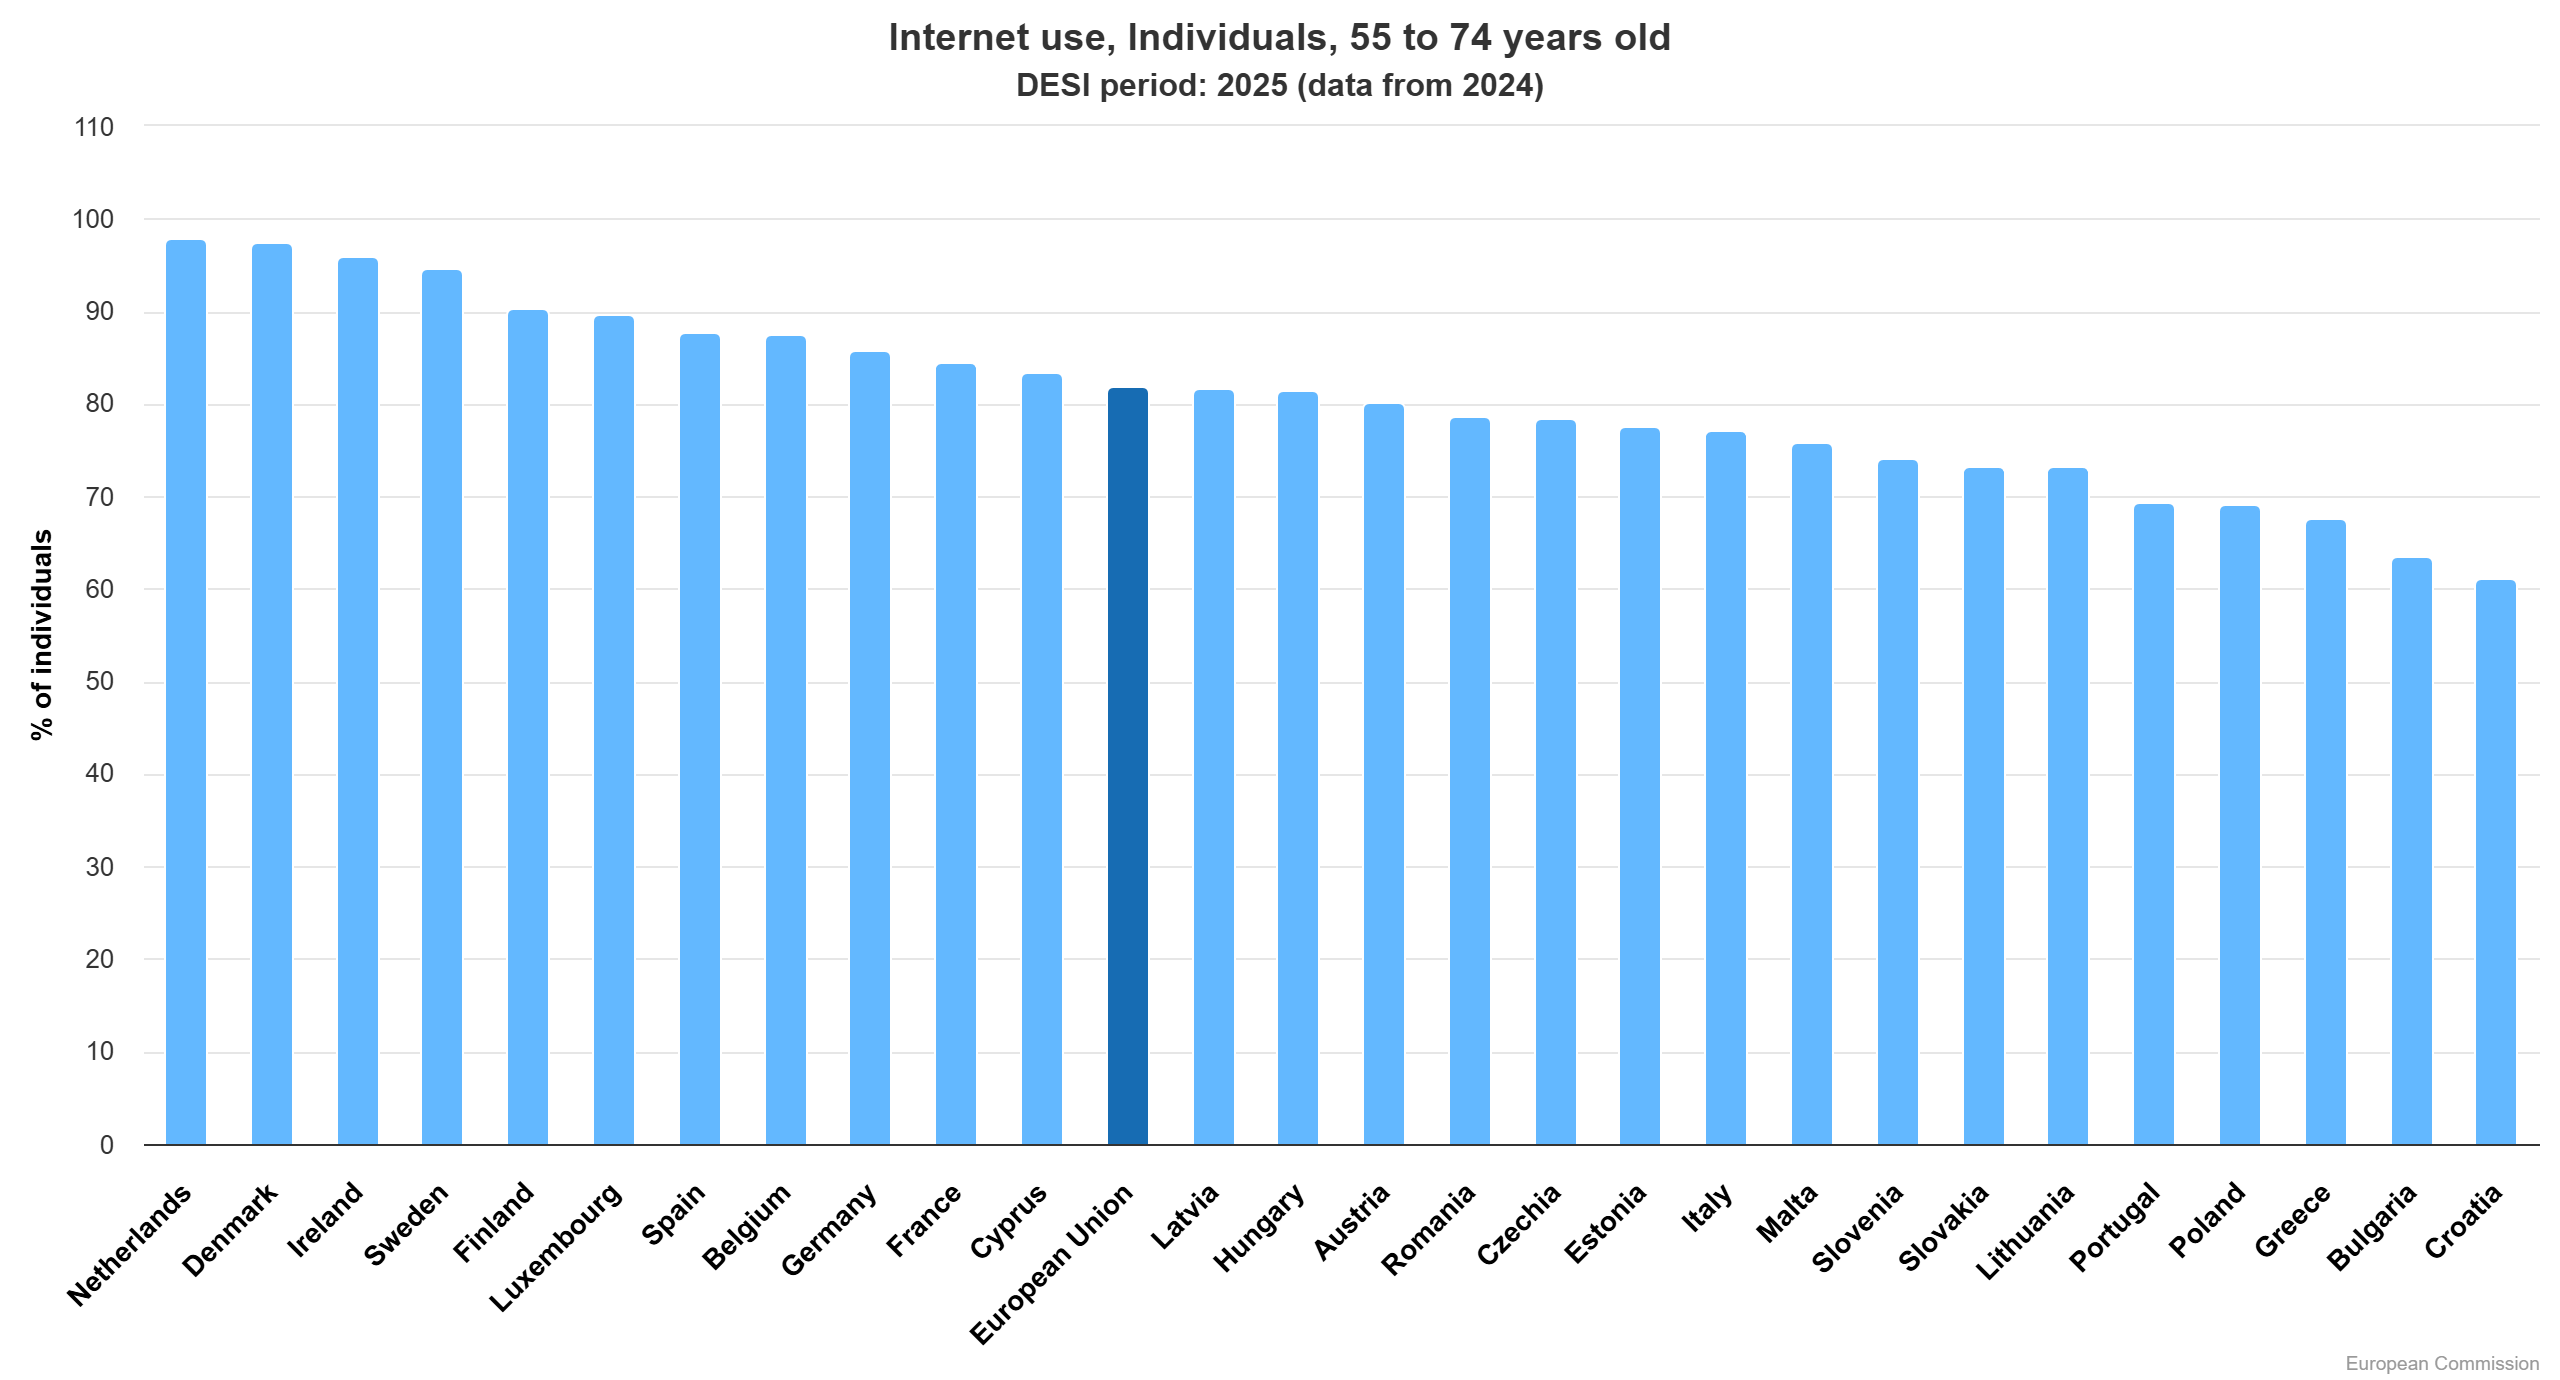
\includegraphics[width=6.3cm]{figures/internet-use-individuals-54-74.png} }}%
		\caption{Dimensão Capital Humano, 2024 \cite{itu2024facts}}%
		\label{fig:capitalhumano}%
	\end{figure}

O mesmo relatório enfatiza que, apesar do avanço nas competências básicas, são necessários esforços redobrados para que Portugal atinja a meta europeia de 80\% da população com competências digitais básicas até 2030 e supere os seus défices na dimensão global do Capital Humano \cite{DESI2024}.

Pode, assim, concluir-se que esta falta de competências básicas foi agravada pela pandemia. De acordo com o relatório ``\textit{Youth \& COVID-19: Impacts on jobs, education, rights and mental well-being}'' \cite{impactocovideducacao}, 65\% dos jovens afirmaram ter aprendido menos desde o início da pandemia, devido à transição das aulas presenciais para o regime \textit{online} durante o confinamento. Apesar dos esforços para manter os estudos, metade considerou que ficou para trás, e 9\% temeu reprovar devido às dificuldades sentidas. A situação foi ainda mais grave entre os jovens de países com baixos rendimentos, devido ao acesso limitado à Internet, à falta crítica de equipamentos e, em alguns casos, à ausência de um espaço adequado para aprendizagem em casa \cite{impactocovideducacao}.

Com base nestes resultados, o estudo conclui que ``os desafios colocados pela transição para o ensino fora da sala de aula e em casa foram enormes.''. Mesmo quando as instituições conseguiram fazer a transição para a aprendizagem \textit{online}, os professores, formadores e estudantes podem não ter tido a capacidade de ``garantir a continuidade da aprendizagem''. Entre os factores que dificultam a eficácia do ensino \textit{online} contam, como já foi referido: baixos níveis de acesso à Internet; lacunas nas competências digitais; incapacidade de ensinar e aprender à distância; falta de equipamento informático em casa; falta de espaço; falta de materiais preparados para o \textit{eLearning}; e falta de trabalho de grupo e de contacto social - ambos componentes fundamentais do processo de aprendizagem.

Enquanto docente do ensino secundário e director de turma, com responsabilidades tanto junto do corpo docente como dos alunos, foi possível observar diversas dificuldades enfrentadas pelos estudantes, nomeadamente a ausência de um computador pessoal, a falta de acesso à Internet ou a existência de uma ligação extremamente lenta. Registaram-se, inclusivamente, casos de alunos que participaram nas aulas através do telemóvel. Do lado dos docentes, verificou-se um desafio considerável, sobretudo devido à falta de experiência prévia no ensino à distância e às dificuldades em identificar e utilizar adequadamente as diversas ferramentas \textit{online}. A correspondente curva de aprendizagem revelou-se lenta e exigente para muitos deles.

Esta realidade não se verificou apenas em Portugal, mas estendeu-se a nível global. Em meados de março de 2020, escolas e instituições de ensino em todo o mundo foram encerradas, e os alunos de todos os níveis passaram a assistir às aulas e a interagir com os professores através de videoconferências e outras ferramentas digitais. A \acrfull{unesco} apoiou a implementação de programas de ensino à distância em larga escala, recomendando aplicações e plataformas educativas gratuitas que pudessem ser utilizadas por escolas e professores para assegurar a continuidade pedagógica. A organização partilhou ainda boas prácticas para o uso de tecnologias móveis de baixo custo com fins educativos, com o objectivo de atenuar os impactos negativos da interrupção do ensino presencial \cite{unesco}.

Do ponto de vista da práctica pedagógica em contexto de sala de aula, especialmente nas disciplinas laboratoriais - como é o caso da Electrónica -, as aulas à distância mostraram-se particularmente desadequadas. Um exemplo evidente foi a substituição do contacto directo com materiais físicos, como a placa branca (também conhecida por \textit{breadboard} ou placa de ensaio) e os componentes electrónicos reais, pelo uso de simuladores \textit{online}, como o \textit{Multisim}~\cite{multisim} e o \textit{Falstad} \cite{falstad}. Embora estes simuladores já fossem utilizados como complemento às actividades presenciais, o seu uso exclusivo limitou fortemente a experiência práctica dos alunos, que deixaram de poder manipular fisicamente os circuitos - um aspecto central para a consolidação de competências técnicas nesta área. Em Agosto de 2020, numa citação incluída num artigo publicado no \textit{Diário de Notícias}, um aluno afirmava:
\begin{center}
    ``\textit{As aulas de laboratório foram as que menos sentido fizeram para mim, pois fazer relatórios e cálculos sobre experiências que não fizemos, sem adquirir/desenvolver as competências e técnicas que é suposto esta componente da disciplina nos dar, é um pouco ridículo}'' \cite{impactonegativocovid}.
\end{center}

Assim, a resposta à questão colocada anteriormente é: não, ninguém estava preparado para estas mudanças nem para o ensino \textit{online} e o \textit{eLearning}.

Nos últimos anos, Portugal tem investido significativamente, não só na educação digital mas também em diversas iniciativas, reconhecendo a importância das competências digitais para o futuro dos seus cidadãos e para a competitividade do país. No contexto nacional, o \acrfull{prr} previu a entrega de computadores portáteis a todos os alunos e docentes do ensino básico e secundário. Estava inicialmente prevista a distribuição de 600 mil computadores com acesso à Internet; contudo, a implementação ficou aquém das expectativas. Em 2023, a \acrfull{cnaprr} classificava como ``preocupante'' a evolução da iniciativa Escola Digital \cite{PRREntregacomputadores}. Até essa data, apenas cerca de 70\% dos equipamentos tinham sido efectivamente entregues. A principal razão prendeu-se com a exigência de um compromisso por parte dos encarregados de educação, que teriam de reembolsar o valor dos equipamentos caso não os devolvessem nas mesmas condições, dificultando a aceitação do programa. Acrescem ainda dificuldades logísticas identificadas por diversas escolas \cite{PRREntregacomputadores}. A estas limitações somam-se decisões políticas recentes que não parecem alinhar-se com os objectivos da transição digital. No início do ano lectivo de 2024/2025, foi reportado que milhares de alunos e docentes ficaram sem acesso aos \textit{hotspots} de Internet integrados nos \textit{kits} digitais escolares, medida justificada pela tutela como sendo transitória, mas que afectou directamente a continuidade digital no processo de ensino-aprendizagem. Esta alteração comprometeu não só a equidade no acesso, como também a eficácia dos recursos já distribuídos, dificultando o cumprimento dos objectivos traçados no Plano de Acção para a Transição Digital~\cite{ExecutiveDigest2024}.

O Plano Nacional de Competências Digitais (INCoDe.2030)~\cite{incode2030}, foi lançado em 2017 e constitui uma iniciativa estratégica do governo português com o objectivo de reforçar a literacia digital da população em geral. Estruturado em cinco eixos fundamentais - inclusão, educação, qualificação, especialização e investigação - o plano orienta um conjunto alargado de políticas públicas e iniciativas destinadas à promoção das competências digitais ao longo da vida. No âmbito deste plano foi criado o Observatório das Competências Digitais, uma plataforma de monitorização e análise que sistematiza e disponibiliza informação sobre as diversas ações e programas desenvolvidos no contexto do INCoDe.2030. Entre as iniciativas registadas pelo Observatório destacam-se projectos como ``Eu Sou Digital'', \textit{Apps for Good} e a iniciativa Ensico~\cite{observatorio2030}, representando exemplos concretos da operacionalização das metas estabelecidas pelo plano.

Em junho de 2025, a \acrshort{cnaprr} apresentou o quinto relatório relativo à execução do \acrshort{prr}. Este documento destaca os investimentos estratégicos associados à transição digital, bem como os resultados esperados, entre os quais se salientam a ``\ldots diminuição das desigualdades no acesso à tecnologia\ldots '' e ``\ldots melhorias na eficiência e qualidade dos processos de ensino\ldots''. Entre os investimentos identificados no relatório, orientados para a modernização das infraestruturas escolares, incluem-se: a aquisição de videoprojectores, a implementação dos \acrfull{led}, a ampliação das redes de área local sem fios, o reforço da conectividade à Internet através da rede alargada da Educação, bem como o Projeto Redimensionar a ligação das escolas a essa rede, com vista à melhoria da largura de banda e da fiabilidade do acesso \cite{cnaprr2025}.

Complementarmente, no estudo de caso desenvolvido por Wastiau et al. (2024) \cite{estrategiatransdigital}, são analisadas outras iniciativas que sustentam a transição digital no sector educativo, com destaque para o Programa Nacional de Promoção do Sucesso Escolar (PNPSE), a Estratégia Nacional de Educação para a Cidadania (ENEC), consagrada no Decreto-Lei n.\textsuperscript{o}~55/2018, e o Regime Jurídico da Educação Inclusiva, estabelecido pelo Decreto-Lei n.\textsuperscript{o}~54/2018. Segundo os autores, estas políticas ``\ldots orientam e são, por sua vez, fortalecidas pela estratégia de transição digital adoptada em 2020.''~\cite{estrategiatransdigital}.

Os desafios para alunos e professores foram enormes, a adaptação ao processo de ensino/aprendizagem \textit{online} teve de ser feita muito rapidamente e os recursos digitais tornaram-se a ``tábua de salvação'' da educação. No entanto, as oportunidades que as tecnologias digitais oferecem vão muito além do apoio de emergência utilizado durante a pandemia. Actualmente, está disponível um grande número de possibilidades, novas respostas para ``o quê'', ``como'' e ``quando'' as pessoas aprendem \cite{oecd_state_2021}.

A forma de pensar dos estudantes de hoje é também muito diferente da de há trinta anos. De uma forma mais particular, o pensamento mudou muito desde que a Internet e os recursos digitais começaram a tornar-se massivos. É essencial que os alunos possam aceder à tecnologia e utilizá-la para se desenvolverem ainda mais e a lição mais importante de todas é: permitir-lhes compreender o que fazer com a informação e os recursos que estão à sua disposição de tantas formas diferentes. Esta nova adaptação educativa (ou deveria chamar-se ``evolução''?) ``também adapta a aprendizagem aos estilos de aprendizagem pessoais com uma granularidade e precisão muito maiores do que qualquer ambiente de sala de aula tradicional pode fazer. Do mesmo modo, laboratórios virtuais dão aos alunos a oportunidade de conceber, realizar e aprender com as experiências, em vez de se limitarem a aprender sobre elas.'' \cite{oecd_state_2021}.

Por outro lado, os professores devem desenvolver a sua literacia digital, para melhor dominarem estas novas ferramentas na sala de aula, de forma a ajudarem os alunos a construírem o seu próprio conhecimento. Assim, é evidente que a Educação, como um todo, precisa de se inserir neste contexto que está cada vez mais presente no quotidiano de todos. O mundo é cada vez mais dominado pela tecnologia (\ldots e, nos tempos actuais, o domínio da Inteligência Artificial já se faz sentir). Milhares de milhões de dispositivos físicos em todo o mundo estão agora ligados à Internet, todos recolhendo e partilhando dados. Actualmente, os circuitos integrados - ou microprocessadores e microcontroladores, consoante a aplicação - são produzidos a baixo custo, e a ubiquidade das redes sem fios permite ligar practicamente qualquer objecto, desde algo tão pequeno como um comprimido até algo tão grande como um avião. A esta rede global de dispositivos interligados, com capacidade de recolher e trocar dados em tempo real, dá-se o nome de Internet das Coisas (\acrfull{iot}) \cite{IoT}.

Por conseguinte, a informação e os recursos estão “na ponta dos dedos de todos” e à distância de um clique.

\begin{center}
    ``\textit{Chegou o momento de os países aproveitarem as lições da pandemia para reconfigurarem as pessoas, os espaços, o tempo e a tecnologia, de modo a criarem ambientes educativos mais eficazes e eficientes}'' \cite{thestateofeducation}.
\end{center}

Se reflectirmos sobre esta ideia em contexto educativo e acrescentarmos o facto de o ensino da Electrónica em Portugal, ao nível do ensino secundário, passar pelo ensino profissional e se o objectivo é a evolução e inovação no processo de ensino/aprendizagem, é necessário proporcionar a todos os intervenientes as condições e ferramentas necessárias para que o trabalho possa ser desenvolvido e, consequentemente, os alunos realmente aprendam. Practicamente todas as aprendizagens e futuros empregos exigirão um certo nível de competências e aptidões digitais. A constante evolução tecnológica exige o desenvolvimento de competências ao longo da vida \cite{Digitale13:online}.

O esforço na evolução da educação digital em Portugal, e consequente aumento do indíce \acrshort{desi} de Capital Humano,  pode ser aferida pelas crescentes iniciativas governamentais e adopção de tecnologias digitais nas escolas e universidades. Este esforço é materializado através de várias iniciativas e programas governamentais que visam aumentar a literacia digital, integrar a tecnologia no sistema educacional, capacitar professores e preparar os estudantes para a era digital. ``As medidas de apoio aos objectivos digitais representam um montante que corresponde a 22\% da dotação total do plano, ultrapassando o limiar de 20\% definido pela regulamentação europeia'' \cite{Transicaodigitalprr}.
\begin{comment}
SE CALHAR TERMINAVA AQUI

No entanto, no meio destas oportunidades criadas, ainda há alguns desafios que precisam de ser ultrapassados. A desigualdade no acesso à tecnologia ainda é uma barreira significativa \cite{desigualdades}, especialmente em áreas rurais e entre famílias de baixos rendimentos. A formação contínua dos professores também necessita de maior suporte, assim como a atualização constante dos recursos digitais disponíveis \cite{afirmacaodigital, problemasprovas}. 
\end{comment}

\section{eLearning e abordagem STEM} %The main chapter title
%\chaptermark{O \textit{Template}}	%Short version for page header. Comment if not needed
\label{sec:elearningstem}	%For referencing the chapter elsewhere, use \ref{Chapter2} 

%%%%%%%%%%%%%%%%%%%%%%%%%%%%%%%%%%%%
Após a análise dos investimentos em infraestruturas digitais e das políticas educativas associadas à transição digital, importa agora aprofundar duas abordagens fundamentais neste contexto: o \textit{eLearning} e a abordagem \acrshort{stem}. Estas abordagens, embora distintas nas suas origens, revelam-se hoje profundamente interligadas, sobretudo quando integradas em ambientes de aprendizagem mediados por tecnologia.

A evolução recente da educação digital foi particularmente acelerada com a pandemia da \acrshort{covid-19}, que impulsionou a adopção de recursos digitais a uma escala sem precedentes. O \textit{eLearning}, até então complementar ao ensino presencial, tornou-se não apenas comum, mas necessário. Assistiu-se, assim, a uma migração generalizada do modelo tradicional de sala de aula para ambientes virtuais de aprendizagem, baseados em plataformas digitais. Esta transformação não apenas democratizou o acesso à educação, como também ampliou as possibilidades pedagógicas, abrangendo formatos como cursos \textit{online}, laboratórios virtuais e remotos e simuladores digitais. Neste contexto, torna-se pertinente reflectir sobre como o \textit{eLearning} se articula com abordagens como a \acrshort{stem}, especialmente no que se refere ao desenvolvimento de competências digitais, científicas e tecnológicas. A integração de laboratórios remotos, simuladores e ambientes experimentais digitais surge, assim, como um eixo estruturante para uma educação inovadora, inclusiva e tecnicamente actualizada.

\subsection{Uma questão de conceitos}
O conceito de \textit{eLearning} tem sido amplamente discutido, sendo objecto de múltiplas definições ao longo das últimas décadas. Esta diversidade não é apenas semântica, mas reflete também os diferentes contextos de aplicação e as abordagens teóricas subjacentes. Em 2004, Jay Cross no seu artigo ``\textit{An Informal History of eLearning}''~\cite{jaycross}, discute a natureza fluida e a evolução deste modelo. Cross apresenta o \textit{eLearning} como uma visão para a transformação da formação empresarial, destacando o seu carácter informal e descentralizado.  No entanto, num estudo intitulado ``O e-Learning no Ensino Superior: um caso de estudo'' \cite{eLearningenssup}, Magano et al. (2008), generalizam a definição dada por Maria João Gomes no seu artigo sobre reflexões em torno do \textit{eLearning} \cite{gomes_e-learning_2005}, considerando que este ``(\ldots) corresponderá a qualquer metodologia de ensino/aprendizagem que integre actividades, suportadas por \acrshort{tic}, essenciais para atingir os objectivos de aprendizagem definidos.''. No mesmo artigo, Maria João Gomes defende que ``(\ldots) o termo e-learning deve ser adoptado como menos centrado nos aspectos tecnológicos e mais próximo das potencialidades pedagógicas decorrentes da utilização das ``tecnologias de rede'' na concepção de situações baseadas na interacção e colaboração, no sentido da construção de aprendizagens significativas''.

Assim, é evidente que não existe um consenso unívoco sobre o significado de \textit{eLearning}. Esta multiplicidade de definições resulta das diversas perspetivas, interesses e concepções dos diferentes intervenientes - académicos, técnicos, políticos e pedagógicos - que, de diferentes formas, têm contribuído para o desenvolvimento deste domínio.

Para ilustrar ainda mais essa diversidade de entendimentos, destaca-se a definição apresentada no ``Convite à apresentação de propostas DG EAC/46/02'' \cite{comissao197_07}, que descreve o \textit{eLearning} como ``(...) a utilização das novas tecnologias multimédia e da Internet para melhorar a qualidade da aprendizagem, facilitando o acesso a recursos e serviços, bem como o intercâmbio/interação e a colaboração à distância.''. Esta visão aproxima-se de uma concepção de aprendizagem assente na comunicação e na colaboração \textit{online}, como referida também por Maria João Gomes \cite{gomes_e-learning_2005}.

Uma das principais vantagens do \textit{eLearning} é a flexibilidade que oferece. Os estudantes podem aprender ao seu próprio ritmo e em horários ajustados às suas rotinas, o que é particularmente útil para aqueles que têm outras responsabilidades, como o trabalho ou a apoio à família. Para além disso, \textit{eLearning} pode também ocorrer a partir de qualquer lugar, desde que haja uma ligação à Internet, o que permite aos alunos estudar a partir de casa ou de qualquer outro lugar que lhes seja conveniente. Outra vantagem é que permite o acesso a uma grande variedade de recursos e materiais de aprendizagem, incluindo vídeos, textos, actividades interactivas, fóruns de discussão, laboratórios virtuais e remotos, entre outros. Estes recursos podem ser actualizados e adaptados rapidamente de acordo com as necessidades dos alunos e professores, garantindo que os conteúdos estão sempre actualizados e são relevantes.Além disso pode também ser uma forma eficaz de personalizar a aprendizagem, permitindo que os alunos se concentrem nas áreas em que precisam de mais ajuda e avancem rapidamente nas áreas em que já têm conhecimentos suficientes. As avaliações \textit{online}, por sua vez, permitem diagnosticar competências e conhecimentos, permitindo ao professor ajustar e adaptar os conteúdos e as actividades de aprendizagem às necessidades individuais de cada estudante.

Para as instituições de ensino em Portugal, o \textit{eLearning} pode ajudar a reduzir os custos, eliminando a necessidade de espaço físico e equipamento adicionais, assim como, também pode ajudar a alcançar um público mais vasto de alunos, especialmente aqueles que não têm acesso ao ensino presencial devido a restrições geográficas, financeiras ou outras. Permite, também, que as instituições de ensino em Portugal ofereçam educação de qualidade a um custo mais baixo, dando a possibilidade a que mais pessoas tenham acesso à educação. Por último, pode contribuir para melhorar a qualidade do ensino em Portugal, permitindo que os alunos aprendam de forma mais eficaz e eficiente. Os professores podem monitorizar os progressos dos alunos em tempo real, fornecendo \textit{feedback} imediato e adaptando os conteúdos às suas necessidades. Além disso, o \textit{eLearning} pode ajudar a promover a colaboração entre alunos e professores, permitindo-lhes trabalhar em conjunto em projectos e actividades de grupo, independentemente da sua localização física. Embora existam desafios envolvidos na adopção do \textit{eLearning}, os benefícios superam os problemas e é provável que o \textit{eLearning} continue a ser uma parte importante do ensino no futuro.

Tal como foi referido nos parágrafos anteriores, não é objectivo desta dissertação apresentar ou analisar exaustivamente as múltiplas definições e concepções de \textit{eLearning}. O mesmo princípio aplica-se à abordagem \acrshort{stem}. No entanto, torna-se relevante compreender este conceito e a sua evolução ao longo do tempo, sobretudo no contexto da educação digital.

O acrónimo \acrshort{stem} designa a área da Ciência, Tecnologia, Engenharia e Matemática e o conceito vai muito além de uma mera definição. Se tomarmos como ponto de partida o \textit{site} da \acrshort{unesco} \cite{GlossaryUNESCO}, é fácil compreender que as definições dão um sentido lato ao conceito. Citando Gonzalez e Kuenzi (2012) \cite{GonzalezKuenzi} e o \textit{Australian Council of Learned Academies} (ACOLA) 2014 \cite{acola}, verifica-se que consideram essencialmente a ``ocupação'', embora em contextos diferentes. Enquanto a primeira publicação apresenta um diagnóstico de \acrshort{stem} nos \acrfull{eua}, a segunda publicação aborda uma forma de reduzir as lacunas nestas competências. Jonathan Rothwel, no seu artigo, ``\textit{The Hidden STEM Economy}'' \cite{TheHidde2:online}, procura clarificar a ambiguidade deste conceito definindo primeiro conhecimento \acrshort{stem}, e assim ``constata que uma grande parte dos empregos ligados a esta área são técnicos (``\textit{blue-collar}'') e não ``académicos''''. Uma terceira definição - talvez a que melhor se adequa aos objectivos deste trabalho - é apresentada por Mark Sanders no artigo “STEM, STEM Education, STEMmania” \cite{TTTSTEMA77:online}. O autor centra-se especificamente no termo ``\acrshort{stem} education'', fazendo a apologia de uma abordagem integrativa, ou seja, do ensino articulado entre duas ou mais das áreas disciplinares que compõem o acrónimo, ou entre uma dessas áreas e outra de natureza distinta. Esta visão defende, assim, a integração curricular como princípio estruturante, em contraste com perspectivas mais fragmentadas da educação científica e tecnológica.
Em termos gerais, a expressão ``\acrshort{stem} education'' refere-se a actividades educativas desenvolvidas em todos os níveis de ensino - desde a Educação Pré-escolar até ao pós-doutoramento - e em contextos tanto formais (como as salas de aula) como informais (por exemplo, programas pós-escolares ou iniciativas extracurriculares). Nos últimos anos, surgiu uma nova definição baseada na ideia de acrescentar as artes ao currículo, recorrendo a princípios de raciocínio e concepção e incentivando soluções criativas, no que se designa por \acrfull{steam}. No entanto, tal como referido anterioremente, não é objectivo do presente documento desenvolver ainda mais estes conceitos específicos.

Na práctica pedagógica desenvolvida, não só em contexto de sala de aula, mas também em ambientes não formais, os alunos participam em diversos projectos, tanto a nível nacional como internacional, nos quais aplicam os princípios da abordagem \acrshort{stem}. As actividades desenvolvidas são bastante diversificadas - desde o envio de engenhos para a estratosfera até à construção de robôs.
%https://www.esa.int/Education/Teachers_Corner/About_the_e-technology_lab

\subsection{Principais desafios}
Um dos principais desafios enfrentados em Portugal na implementação da abordagem \acrshort{stem} é a falta de recursos e de infraestruturas adequadas. Tal como foi referido anteriormente, e conforme reforçado pelo mais recente relatório do \acrfull{pisa}, da \acrfull{ocde}, muitas escolas continuam sem acesso a laboratórios devidamente equipados e à tecnologia actualizada necessária para um ensino eficaz das ciências e da tecnologia \cite{pisa2022volume2}. Neste âmbito, a insuficiência do investimento na educação em Portugal constitui uma limitação significativa, condicionando a capacidade do país para inovar e desenvolver novas tecnologias \cite{Oquefalt37:online, Faltadei99:online, Odesinve56:online, EDUSTATP20:online, Portugal69:online}.

Adicionalmente, os pontos fracos do sistema educativo português - identificados no relatório da \acrshort{ocde} intitulado ``\textit{Effective policies, Successful Schools}'' \cite{pisa2018volumeV} - incluem a escassez de pessoal não docente, a elevada taxa de retenções, a carência de equipamento informático, a ausência de plataformas de ensino \textit{online} eficazes, o acesso limitado e pouco fiável à Internet, bem como a persistente falta de equidade.

Para além destas limitações estruturais, regista-se igualmente a escassez de profissionais qualificados nas áreas \acrshort{stem}. Num artigo publicado no \textit{site} oficial da \acrshort{ue}~\cite{cedefop}, é referido que ``Em toda a \acrshort{ue}, uma das principais causas do défice de profissionais de \acrshort{tic} e \acrshort{stem} prende-se com a insuficiência da oferta de licenciados do ensino secundário superior e do ensino superior em relação à procura crescente''. Esta escassez está directamente relacionada com a baixa percentagem de profissionais no sector das \acrshort{tic}. De acordo com o Relatório da Década Digital 2024 \cite{DigitalDecade2024}, a percentagem de especialistas em \acrshort{tic} empregados no país é ligeiramente inferior à média da União Europeia (4,6\% contra 4,8\%), com uma diminuição preocupante na representação feminina (20,2\% em 2024, face a 20,4\% em 2021). Este dado evidencia não só um défice quantitativo, mas também um desafio persistente em termos de diversidade e atractividade das carreiras tecnológicas - aspectos intrinsecamente ligados ao reforço do ecossistema \acrshort{stem} nacional. O relatório recomenda, por isso, a adopção de medidas para aumentar o número de especialistas em \acrshort{tic}, bem como o incentivo à participação dos jovens - especialmente das raparigas - no prosseguimento de estudos e carreiras nas áreas tecnológicas. %https://digital-strategy.ec.europa.eu/pt/factpages/portugal-2024-digital-decade-country-report

A pandemia da \acrshort{covid-19} também apresentou desafios adicionais para a implementação do \acrshort{stem}. Com muitas escolas fechadas e com aulas à distância, muitos alunos não tiveram acesso a laboratórios e equipamento especializado necessário para aprender ciência e tecnologia \textit{hands-on}. Além disso, como já foi referido na Secção~\ref{sec:transformaçãodigital}, a pandemia aumentou a desigualdade na educação, com os alunos de famílias com baixos rendimentos a terem menos acesso à tecnologia e aos recursos necessários para acompanhar o ensino à distância \cite{desigualdadespandemia, efeitospandemiadigital}.

Ultrapassar estes desafios não é tarefa simples e exige um esforço concertado por parte de todos os intervenientes no processo educativo. No entanto, é legítimo questionar qual poderá ser, neste contexto, o papel concreto dos professores.

Em primeiro lugar, procurar os recursos cuja utilização em contexto de sala de aula possa, pelo menos, permitir que o processo de ensino-aprendizagem evolua e que estes desafios sejam ultrapassados ou, pelo menos, atenuados: Os recursos ``(\ldots) didácticos parecem estar no centro de tudo, os professores precisam deles para ajudar no seu ensino e os alunos precisam deles para os ajudar na sua aprendizagem.''~\cite{virtuallabng}. Por outro lado, num inquérito \cite{pearson} realizado em nome da Pearson\footnote{https://plc.pearson.com/} pela The Harris Poll\footnote{https://theharrispoll.com/}, envolvendo 7038 pessoas com idades compreendidas entre os 16 e os 70 anos em todo o mundo, verificou-se que 78\% dos inquiridos acreditavam que a aprendizagem \textit{online} daria às pessoas mais fácil acesso a uma educação de qualidade. 

Pelo que foi dito anteriormente e conhecendo bastante bem a realidade do ensino secundário por trabalhar com alunos que, na sua maioria vão directamente para o mundo do trabalho, pode-se concluir que a educação enfrenta vários desafios, nomeadamente a necessidade dos professores, em particular, se manterem actualizados em relação às tecnologias emergentes, bem como serem capazes de preparar os alunos para as exigências do mercado de trabalho em constante evolução. No entanto, este não será o maior desafio. Existem vários e graves problemas a montante que tornam o processo de ensino/aprendizagem muito difícil. Este não é apenas um problema das escolas secundárias, abrangendo também o ensino universitário. De facto, podemos referir como um problema grave as dificuldades financeiras~\cite{dificuldadesfinanciamento, Financiamentoprofissional, Educacaofinanciamento} das escolas e universidades, que limitam o acesso dos alunos a equipamentos e materiais necessários essenciais nomeadamente para as aulas laboratoriais: computadores actualizados, software, etc. Uma das consequências desta limitação é a falta de ligação entre a teoria e a práctica. Muitas vezes, os alunos são expostos a uma grande quantidade de informação teórica, mas não têm a oportunidade de aplicar esses conhecimentos em projectos práticos. Este facto pode levar a uma falta de compreensão sobre como as teorias se aplicam na vida real e pode dificultar a transferência de conhecimentos para a práctica profissional.

%Como ultrapassar este problema?

% \vspace{1cm}

% \vspace{5pt}
% \hrule
% \vspace{6pt}
% \textcolor{red}{Secção - decidir se vale a pena - \textbf{A REVER}} 

% \textbf{eLearning and laboratories}
% Laboratory activities have long had a distinctive and central role in the science curriculum and science educators have suggested many benefits come from from engaging students in science laboratory activities \cite{Hofstein}.

% Vários estudos confirmam  (...)


% \textbf{Ensino profissional pode ser traduzido em ``vocacional education''}

% \vspace{1cm}

% \vspace{5pt}
% \hrule
% \vspace{6pt}

%In chapter \ref{Chapter2} a question was made: ``How to overcome this problem?'', being ``this problem'' the financial difficulties which prevents the development of a more capable teaching. This is reflected in the difficulties and lack of resources in laboratory classes.

%\section{eLearning future}
%\textcolor{magenta}{\textbf{\underline{NOTA:} Irrelevante. A REVER}}

%Já vimos nos capítulos/secções anteriores que o \textit{eLearning} é uma mais-valia em contexto de sala de aula. No enquadramento deste ``Estado da Arte'', pode-se referir, mais especificamente, que o \textit{eLearning} pode substituir ou complementar a falta de laboratórios reais. Obviamente que o conceito do ensino à distância é muito abrangente e poderá ser exptrapolado para lá de um mero complemento laboratorial, inclusive no mundo empresarial. %De facto, cada vez mais empresas
%https://www.emerald.com/insight/content/doi/10.1108/10748120410564458/full/html

%https://eLearningindustry.com/eLearning-and-the-future-of-education

%\section {Educação STEM Education | Abordagem STEM}

% \sout{No entanto, apesar destes desafios e dificuldades, existem esforços significativos para impulsionar a implementação do \acrshort{stem} em Portugal. O governo tem trabalhado para aumentar o investimento em investigação e desenvolvimento, bem como para criar programas e iniciativas que incentivem os estudantes a escolher a ciência e a tecnologia. Além disso, muitas empresas e organizações estão a colaborar, através de protocolos, com escolas e universidades para fornecer recursos e oportunidades de aprendizagem práctica em \acrshort{stem}.}

Para ultrapassar os desafios da implementação do \acrshort{stem} em Portugal, é importante que o país continue a investir em recursos e infraestruturas adequados ao ensino e aprendizagem das ciências e tecnologias. Além disso, é necessário sensibilizar para a importância do \acrshort{stem} para o futuro de Portugal e proporcionar oportunidades de carreira atractivas para os licenciados nestas áreas. Finalmente, é também importante que Portugal trabalhe para manter o seu talento científico e tecnológico no país, em vez de o perder no estrangeiro: ``Portugal perde 4 mil cérebros por ano'' \cite{Cerdeira2020}.

% \vspace{1cm}

% \vspace{5pt}
% \hrule
% \vspace{6pt}
% \textcolor{blue}{\textbf{\underline{NOTA:} Esta parte pode ser enquadrada numa conclusão deste capítulo para dar seguimento aos laboratórios - A REVER }}

% Concluir que o stem é importante, há desafios, dificuldades, no âmbito deste texto enquadrar com os laboratórios, nas escolas dificuldades em montar laboratórios, fracos recursos...

% Em Portugal, a aplicação do STEM é um desafio.
% STEM passa pelos professores, mais trabalho, mais domínio de todos os atributos, os professores podem (e têm) dificuldades em dominar as várias áreas do STEM

% \textcolor{blue}{Faz sendido? Terminar esta secção com o parágrafo abaixo? - \textbf{A REVER}}

Esta forma de ensino não só faz a integração das áreas do conhecimento, como também permite ao aluno usá-las para conexões na resolução de problemas diários. A aprendizagem é amplamente beneficiada com a interdisciplinaridade. Além disso, nesta metedologia de ensino, os alunos aprendem a colaborar uns com os outros.

%https://www.engkids.com.br/site/artigos/o-que-e-stem-e-quais-seus-impactos-na-educacao/

\section{Laboratórios na educação}
\label{Laboratóriosnaeducação}

\begin{center}
    \textit{``Teoria sem práctica é utopia,}

    \textit{práctica sem teoria é rotina.''}

    Anónimo\footnote{Como curiosidade, esta frase estava afixada num cartaz na sala de aula de eletrónica do 8\textsuperscript{o}~ano, no ano lectivo de 1985/86.}

\end{center}
Um dos pontos-chave do ensino profissional consiste em preparar os alunos para o mundo do trabalho. A ascensão da \gls{industria40} levou a que mais instituições de ensino adoptassem os laboratórios remotos como uma alternativa contemporânea para o desenvolvimento das competências técnicas e sociais exigidas a estudantes e formadores na área da engenharia \cite{EvaluationRemoteVirtualE-Learning}.

A investigação sobre a eficácia do ensino e da aprendizagem em ambiente laboratorial\footnote{\label{Hofstein}A investigação conduzida por Hofstein \cite{Hofstein} incide sobre laboratórios de ciências, nomeadamente de Química. No entanto, as conclusões podem ser adaptadas ao caso particular dos laboratórios de Electrónica.} remonta à década de 1960 e existem numerosos estudos, ensaios e teses de doutoramento sobre esta temática. Algumas observações particularmente relevantes foram destacadas nos trabalhos de Hofstein \cite{Hofstein}:
\begin{itemize}
    \item As actividades laboratoriais escolares têm potencial especial como meios e estratégias para ensinar e aprender que podem promover importantes resultados de aprendizagem das ciências para os alunos;

          (Este facto é comprovado nas aulas prácticas dos meus alunos. Estes sentem-se muito mais motivados para aprender utilizando qualquer tipo de recurso, quer seja um laboratório real ou um simulador \textit{online}).
    \item Os professores precisam de conhecimentos, competências e recursos que lhes permitam ensinar eficazmente em ambientes de aprendizagem prácticos;

          (Isto está de acordo com o que foi mencionado na secção anterior: Os professores devem desenvolver a sua própria literacia digital. Esta adaptação está a revelar-se um grande desafio).
    \item As percepções e os comportamentos dos alunos no laboratório de ciências são muito influenciados pelas expectativas e prácticas de avaliação dos professores e pela orientação do guia de laboratório, das fichas de trabalho e dos meios electrónicos associados;

          (Obviamente isto requer muito trabalho, empenho e dedicação, e os professores também precisam de motivação e das condições necessárias para poderem desenvolver este tipo de ensino. Em Portugal, sabe-se que vivemos tempos de incerteza relativamente a todas estas condições e situações.).

    \item Os professores precisam de formas de descobrir o que os seus alunos estão a pensar e a aprender no laboratório de ciências e na sala de aula.

          (Precisam de fazer uma avaliação formativa, cujo objectivo não é atribuir classificações/dar notas aos alunos, mas determinar o que aprenderam e como chegaram lá, o que não aprenderam e porque é que isso aconteceu. Assim, poderão encontrar estratégias/recursos para ajudar os seus alunos a ultrapassar os obstáculos que vão surgindo ao longo do processo.).
\end{itemize}
No âmbito da sua investigação, Hofstein reúne diversas reflexões relevantes sobre o papel do laboratório no ensino das ciências.    
Entre os contributos destacados, merece particular atenção a afirmação de Bybee  (2000), citado por \cite{Hofstein} segundo a qual ``Se usado correctamente, o laboratório tem o potencial de ser um meio importante para introduzir os alunos nos conhecimentos e competências conceptuais e processuais centrais da ciência.''. Este é um ponto particularmente relevante, uma vez que a investigação tem demonstrado que as experiências prácticas em laboratório desempenham um papel central - ou mesmo \textit{O} papel central - na educação científica, como referido por Hofstein e Lunetta (2004), citados em \cite{BRINSON2015218}. Esta importância deve-se, em grande medida, ao impacto significativo que essas actividades têm nos resultados da aprendizagem e no desempenho dos estudantes, bem como à sua eficácia na preparação para a futura actividade profissional, como referem Basey et al. (2008), também citados em \cite{BRINSON2015218}.

%\textsuperscript{o}~
Em Portugal, o estudo da Electrónica no ensino secundário é, em grande parte, desenvolvido através do ensino profissional. Este tipo de ensino não só permite que os alunos ingressem no ensino superior com conhecimentos e competências laboratoriais adequadas, como também lhes proporciona as ferramentas necessárias para enfrentarem, com maior preparação, as exigências do mercado de trabalho \cite{anqep}. É evidente, contudo, que esta premissa só se concretiza mediante um ensino eficaz e, subsequentemente, uma aprendizagem efectiva baseada na utilização activa dos laboratórios.

Ao longo de uma carreira com mais de 20 anos como professor de Electrónica, leccionando turmas do 10.\textsuperscript{o} ao 12.\textsuperscript{o}~ano, têm sido utilizadas diversas ferramentas digitais como complemento das prácticas laboratoriais, nomeadamente os já referidos \textit{Multisim} \cite{multisim} (tanto em versão \textit{online} como \textit{stand-alone}) e o \textit{Falstad} \cite{falstad}.

No entanto, devido a dificuldades de vária ordem - nomeadamente de natureza económica - que as escolas têm enfrentado ao longo dos anos, gerando constrangimentos materiais significativos, tornou-se necessário desenvolver a pesquisa e a utilização de novas ferramentas digitais, ou, se assim lhes quisermos chamar, laboratórios virtuais e/ou simuladores. Estas limitações, aliadas ao surgimento da pandemia da \acrshort{covid-19} e à consequente transformação das aulas presenciais em aulas virtuais, intensificaram ainda mais a necessidade de procurar novas soluções digitais, para além das já referidas nos parágrafos anteriores.

É, pois, inquestionável a importância das prácticas laboratoriais nas ciências - ou no caso particular desta dissertação - nas aulas prácticas de Electrónica, tanto no Ensino Secundário como no Ensino Superior. A tentativa de mitigar as dificuldades já referidas neste capítulo levam à procura de soluções alternativas. Vários estudos sugerem que os laboratórios virtuais e remotos surgem como duas soluções que podem ajudar a ultrapassar a falta de laboratórios reais ou a falta de recursos nos laboratórios reais \cite{ImpactRemoteLabTeachingPractices, developremotelabs, HERADIO20161, POTKONJAK2016309}.

% Ver este estudo para complementar
%https://www.sciencedirect.com/science/article/pii/S0360131518301878?via%3Dihub

\subsection{Tipos de laboratórios} %The main chapter title
%\chaptermark{O \textit{Template}}	%Short version for page header. Comment if not needed
\label{sec:tiposlaboratorios}
No contexto educativo e científico, existem diversos tipos de laboratórios, cada um atendendo a diferentes necessidades e objectivos. Os laboratórios são espaços cruciais para a educação, pesquisa e inovação, proporcionando ambientes onde teorias podem ser testadas e conceitos podem ser explorados de maneira práctica \cite{Hofsteinfoundations}. Os principais tipos incluem laboratórios físicos tradicionais, laboratórios virtuais e laboratórios remotos.

Os laboratórios físicos, virtuais e remotos oferecem diferentes vantagens e propõem diversos desafios, sendo frequentemente utilizados de maneira complementar. Os laboratórios físicos tradicionais proporcionam uma experiência práctica essencial, permitindo a manipulação directa dos materiais e equipamentos. Os laboratórios virtuais oferecem uma alternativa segura e económica, ideal para a simulação e modelagem de conceitos complexos. Já os laboratórios remotos combinam os benefícios dos dois, permitindo o controle de equipamentos reais à distância e facilitando a colaboração global. Sendo assim, cada tipo de laboratório desempenha um papel crucial na educação e na investigação e a escolha entre eles depende das necessidades específicas da disciplina, dos recursos disponíveis e dos objectivos pedagógicos. A integração desses diferentes tipos de laboratórios pode proporcionar uma experiência de aprendizagem rica e diversificada, preparando melhor os alunos para os desafios do mundo real e do ambiente académico \cite{BRINSON2015218, ImpactRemoteLabTeachingPractices, Hofsteinfoundations}.

Importa, nesta fase, apresentar uma classificação geral dos laboratórios - ainda que esta não seja consensual. De facto, não existe uma normalização padrão amplamente aceite quanto à forma como estes conceitos são definidos. Como exemplo desta falta de uniformidade, uma possível forma de classificar os laboratórios encontra-se representada na Figura~\ref{fig:classificaçãoHeratio}. Segundo Heradio \textit{et al.} (2016) \cite{HERADIO20161} os laboratórios podem ser divididos consoante a sua localização: locais ou remotos.

\begin{figure}[hbtp]
    \centering
    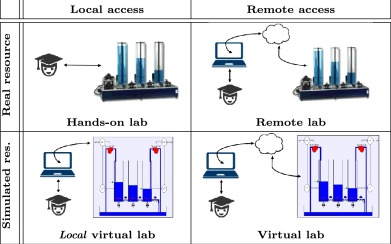
\includegraphics[width=0.65\textwidth]{figures/caracteristica_laboratories.jpg}
    \caption{Tipos de laboratórios consoante a localização, Heradio \textit{et al.} (2016) \cite{HERADIO20161}}
    \label{fig:classificaçãoHeratio}
\end{figure}

Representando de uma outra forma:
\begin{itemize}
    \item Acesso local
          \begin{itemize}
              \item Laboratório real: laboratório físico tradicional, onde os alunos podem realizar experiências prácticas com equipamentos reais (amplamente utilizado em contexto de sala de aula de Electrónica);
              \item Laboratório virtual local: um ambiente digital que simula um laboratório físico, permitindo aos alunos realizar experiências de forma virtual (durante a pandemia, os alunos utilizaram o \textit{multisim} instalado no computador para simular os circuitos);
          \end{itemize}
    \item Acesso remoto
          \begin{itemize}
              \item Laboratório remoto: um laboratório físico real que pode ser controlado à distância, permitindo aos alunos realizar experiências prácticas sem estarem fisicamente presentes (nunca utilizado em contexto de sala de aula de Electrónica);
              \item Laboratório virtual: um ambiente digital que simula um laboratório físico, permitindo aos alunos realizar experiências de forma virtual, independentemente da sua localização (utilizado, também, durante a pandemia mas na versão \textit{online} do \textit{multisim}).
          \end{itemize}
\end{itemize}

Também Zutin \textit{et al.} (2010) \cite{zutinlab2go}, citados por Zapata-Rivera e Larrondo (2017)~\cite{Zapata-Rivera}, classificam os laboratórios de forma idêntica, tal como representado na Figura~\ref{fig:classificaçãozutin}.

\begin{figure}[hbtp]
    \centering
    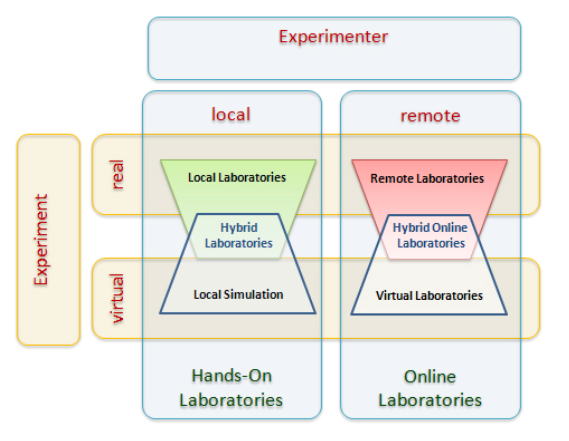
\includegraphics[width=0.65\textwidth]{figures/carac_lab.png}
    \caption{Tipos de laboratórios consoante a localização, segundo Zutin, \textit{et al.} \cite{zutinlab2go}}
    \label{fig:classificaçãozutin}
\end{figure}

Estas duas representações, no entanto, têm algumas diferenças ao nível da nomenclatura, sendo que os autores da segunda representação, introduzem os conceitos de \textit{Hybrid Laboratories} e \textit{Hybrid Online Laboratories}, tradução livre para laboratórios híbridos e laboratórios híbridos \textit{online}, respectivamente. Este tipo de laboratórios são criados através da combinação de laboratórios físicos e/ou laboratórios \textit{online}/remotos \cite{Zapata-Rivera}. Mais uma vez, não é propósito desta dissertação um estudo aprofundado destes conceitos. No entanto, apresentam-se dois casos de configurações híbridas, utilizadas com mais frequência em contexto de sala de aula:

\begin{itemize}
    \item Acesso a um laboratório real (no local) com acesso a um simulador local virtual (configuração realizada com bastante frequência em contexto de sala de aula, onde os alunos testam os circuitos no \textit{multisim} instalado no computador, antes de o testarem na placa branca);
    \item Acesso a um laboratório real (no local) com acesso a um laboratório virtual remoto (configuração usada e idêntica à anterior, com a diferença que o acesso ao laboratório virtual é feito através do \textit{multisim online}.
\end{itemize}

O caso das configurações híbridas \textit{online} nunca foram utilizadas, uma vez que envolvem o acesso a laboratórios remotos e, como já foi referido, nunca foram utilizados  em contexto de sala de aula de Electrónica.

\subsubsection{Uma questão de conceitos}
\label{sec:questaodeconceitos}
Como foi referido na nota\footref{Hofstein}, o estudo de Hofstein incide sobre os laboratórios de ciências. Sendo certo que as suas conclusões podem ser adaptadas ao contexto dos laboratórios no ensino da Electrónica, importa, daqui em diante, clarificar e distinguir os conceitos de ``laboratório virtual'' e ``simulador'' (válidos tanto para versões \textit{online} como locais), uma vez que estas duas definições tendem a sobrepor-se na maioria dos casos. Parte da literatura, trabalhos de investigação e fontes \textit{online} utilizam já o termo ``laboratório virtual'' \cite{BRINSON2015218, virtuallabng, EMaster2024May}, dado que a montagem nesses sistemas é concebida de forma a reproduzir, visual e funcionalmente, um ambiente laboratorial real. No entanto, o objectivo subjacente mantém-se: simular o comportamento de sistemas físicos ou electrónicos. Se se tomar como referência a representação da Figura~\ref{fig:classificaçãoHeratio}, apresentada por Heradio et al. (2016) \cite{HERADIO20161}, os laboratórios virtuais - quer sejam locais, quer \textit{online} - são considerados simuladores, uma vez que permitem simular o comportamento de sistemas físicos ou electrónicos, baseados em modelos matemáticos. No entanto, o inverso nem sempre é válido.

Apresentam-se de seguida três exemplos de tipos de laboratórios virtuais e simuladores (frequentemente utilizados em contexto de sala de aula), que ilustram a distinção entre o que se considera laboratório virtual e simulador, de acordo com a definição anteriormente enunciada. O Tinkercad \cite{tinkercad}, representado na Figura~\ref{fig:tinkercadVL}, é um simulador com características de laboratório virtual, uma vez que a representação dos componentes e a disposição do circuito se aproximam da realidade física de um laboratório tradicional. Por sua vez, o \textit{Multisim} \cite{multisim}, tanto na sua versão \textit{online} como na aplicação instalada no computador, representado na Figura~\ref{fig:multisimSimulador}, é um simulador, dado que a montagem dos circuitos é puramente esquemática, sem qualquer preocupação em replicar a aparência ou o contexto físico de uma montagem real.

\begin{figure}[hbtp]
    \centering
    \begin{subfigure}[hbtp]{0.48\textwidth}
        \centering
        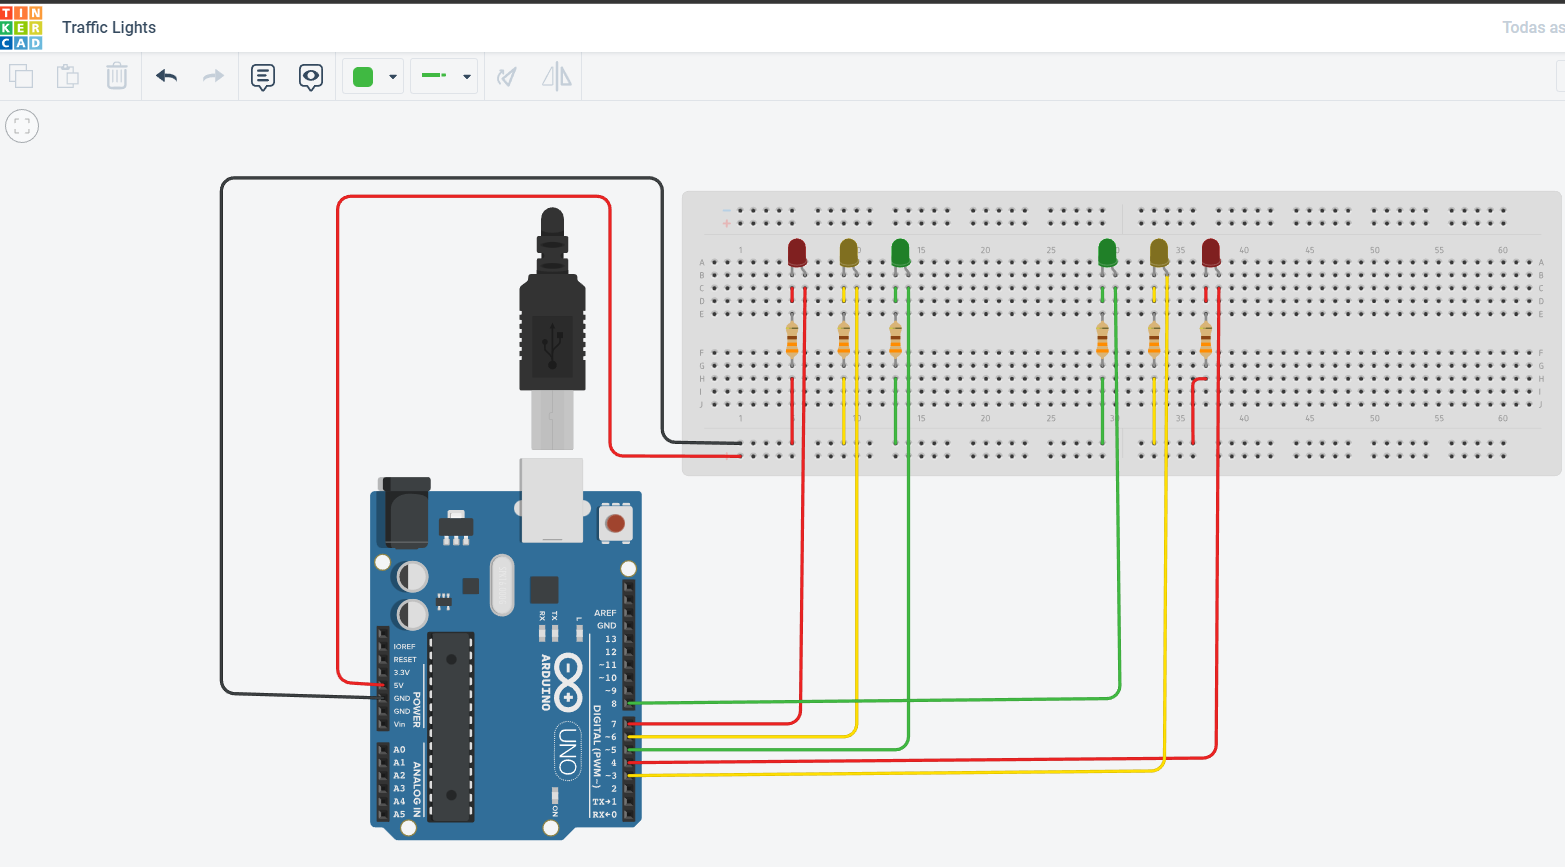
\includegraphics[width=0.9\textwidth]{figures/tinkercad_exemplo.png}
        \caption{\textit{Tinkercad} como laboratório virtual \cite{tinkercad}}
        \label{fig:tinkercadVL}
    \end{subfigure}
    \begin{subfigure}[hbtp]{0.48\textwidth}
        \includegraphics[width=0.9\textwidth]{figures/Astável-schematic.png}
        \caption{\textit{Multisim} como simulador \cite{multisim}}
        \label{fig:multisimSimulador}
    \end{subfigure}
    \caption{Laboratório virtual \textit{vs} simulador}
    \label{fig:tinkercad}
\end{figure}

O \textit{Falstad} \cite{falstad}, representado como exemplo na Figura~\ref{fig:falstad}, é outro dos simuladores \textit{online} amplamente utilizados em contexto de sala de aula. Ao contrário do \textit{Multisim}, que permite ao utilizador construir circuitos a partir de componentes e esquemas eléctricos, o \textit{Falstad} simula o comportamento de circuitos electrónicos com base em esquemas previamente desenhados e estruturados, frequentemente recorrendo a uma \textit{interface} mais simplificada e visualmente acessível. Este simulador é particularmente útil para introduzir conceitos fundamentais de electrónica e teoria de circuitos, permitindo a visualização dinâmica de tensões, correntes e cargas, o que o torna uma ferramenta valiosa no ensino da Electrónica.

\begin{figure}[hbtp]
    \centering
    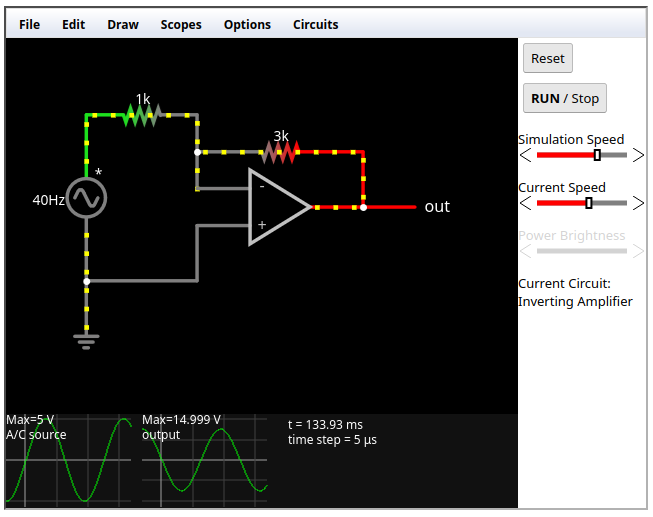
\includegraphics[width=0.6\textwidth]{figures/falstad.png}
    \caption{Simulador \textit{Falstad} (Exemplo) \cite{falstad}}
    \label{fig:falstad}
\end{figure}

Tal como foi referido anteriormente, não há um consenso na forma como são denominadas estas ferramentas. Faiña (2022) \cite{faina}, refere-se ao \textit{Tinkercad} como sendo um simulador, ``Existem vários simuladores destinados a estudantes de eletrónica, como o \textit{TinkerCAD}''. No mesmo trabalho de investigação e refereindo-se ao \textit{Frizing}~\cite{fritzingdown}: ``O simulador apresentado neste artigo é implementado no \textit{Fritzing} (\ldots)''~\cite{faina}. Já Knörig \textit{et al.} (2009) no seu artigo ''\textit{Fritzing: a tool for advancing electronic prototyping for designers}``~\cite{Knorig2009Feb}, referem que ``(\ldots) decidiu permitir ao utilizador documentar o seu protótipo de trabalho baseado numa placa de ensaio com uma metáfora visual que imita a situação do utilizador no mundo real.''. Além disso, ``(\ldots) um laboratório virtual pode ser definido como um ambiente no qual as experiências são conduzidas ou controladas parcial ou totalmente através de operação, simulação e/ou animação por computador, quer localmente, quer remotamente através da Internet.'', tal como referido por Chan e Fok (2023) no seu artigo ``\textit{Evaluating learning experiences in virtual laboratory training through student perceptions}''~\cite{EvaluatingLearningExperiencesVirtualLaboratoryHongKong}. Os laboratórios virtuais oferecem aos alunos um conjunto de oportunidades diferentes, não só como substituto, mas também como complemento dos laboratórios reais.

Assim sendo, e sem prejuízo para os assuntos abordados nesta dissertação, é seguro afirmar que, na ausência de uma uniformização dos critérios relativos às definições e conceitos, todos os laboratórios virtuais podem ser considerados simuladores - reforçando, mais uma vez, que o contrário nem sempre é válido. No contexto da electrónica, optar-se-á por distinguir os laboratórios virtuais como ambientes que procuram replicar visualmente os componentes e a disposição dos circuitos de acordo com a realidade física, ao passo que os simuladores serão entendidos como ferramentas cuja representação é puramente esquemática.

Apesar disso, autores como Heying, Kejie e Jiang (2010) \cite{multisimVLHeying}, bem como Umenne e Hlalele (2020) \cite{multisimVLUmenne}, classificam o Multisim \cite{multisim} como um laboratório virtual nos respectivos trabalhos de investigação.


Após clarificada a distinção entre laboratórios virtuais e simuladores, importa agora enquadrar estes conceitos numa perspectiva particular, considerando os diferentes tipos de laboratórios já utilizados no ensino da Electrónica. Cada uma destas tipologias possui características próprias, vantagens específicas e contextos de aplicação distintos, sendo particularmente relevantes no contexto do ensino da Electrónica e da abordagem \acrshort{stem}.

\subsubsection{Laboratório real}
%\textbf{link para não esquecer}
%https://digital.dge.mec.pt/laboratorios-de-educacao-digital
Neste tipo de laboratórios, os alunos têm à sua disposição os recursos, o equipamento e os materiais físicos necessários para realizar experiências, analisar dados, desenvolver competências de trabalho em equipa e cultivar o interesse pelas ciências. Estas competências revelam-se cruciais para muitas carreiras e profissões, especialmente nas áreas \acrshort{stem}. Além disso, os laboratórios podem ajudar a melhorar a compreensão dos alunos sobre o processo científico e a importância da investigação científica.

No caso específico do ensino secundário - e por experiência própria - uma das soluções encontradas para equipar e desenvolver os laboratórios passa pela aquisição de microcontroladores - como o \gls{arduino} ou \gls{ESP32} - ou o \gls{RaspberryPI}. Estes dispositivos, em conjunto com uma vasta gama de sensores disponíveis no mercado, são amplamente utilizados em ambientes educacionais e de investigação, permitindo a prototipagem rápida, a experimentação práctica e a aprendizagem activa em disciplinas como a Electrónica. A principal vantagem prende-se com a relação custo-eficácia: os microcontroladores e os seus componentes associados são relativamente acessíveis, o que os torna viáveis mesmo em instituições com orçamentos limitados. Acresce a existência de uma comunidade de suporte activa e extensa documentação, factores que facilitam significativamente a aprendizagem e a implementação de projectos por parte de estudantes e docentes. Com estes dispositivos, é possível desenvolver uma variedade quase ilimitada de experiências, desde simples medições de temperatura até projectos avançados de automação, controlo e robótica educativa.
Em Portugal, esta vertente práctica e experimental tem sido amplamente incentivada através de eventos e competições de robótica, que promovem o espírito inovador e empreendedor dos alunos, ao mesmo tempo que reforçam aprendizagens em contexto de sala de aula e de laboratório \cite{roboparty, fnr, cansat}. Entre as mais relevantes, destacam-se:
\begin{itemize}
    \item \textit{RoboParty};
    \item Festival Nacional de Robotica;
    \item \textit{Cansat}.
\end{itemize}

A eficácia do \gls{arduino} como ferramenta pedagógica tem sido amplamente documentada. Yoder (2015) \cite{yoder}, desenvolveu uma alternativa ao laboratório tradicional recorrendo ao \gls{arduino}: ``(\dots) a plataforma Arduino estimulou o interesse e o envolvimento dos alunos desde o início. Vários alunos começaram a alargar os projectos para além dos requisitos na terceira semana de aulas.''. Graven, \textit{et al} (2018), \cite{graven}, citados por Plaza, \textit{et al.} (2018), \cite{plaza} destacam que ``(\ldots) No domínio da educação, o \gls{arduino} é também muito utilizado. Os estudantes de engenharia electrotécnica podem aceder a um laboratório compacto para trabalhar quando e onde quiserem.''. O mesmo autor refere ainda que ``(\ldots) Tal como foi demonstrado por muitas experiências e trabalhos, a robótica combinada com \acrshort{stem} constitui uma forma atractiva de transformar conceitos aborrecidos num processo de aprendizagem divertido.''. Também Marzoli \textit{et al.} (2021), \cite{Marzoli}, no estudo intitulado ``\textit{Arduino: From Physics to Robotics}'', exploram vários pontos e questões, entre os quais se o \gls{arduino} pode melhorar a práctica laboratorial no ensino secundário italiano e mudar as atitudes dos alunos em relação às disciplinas \acrshort{stem}. Os autores questionam ``Como melhorar as prácticas laboratoriais no ensino secundário, tendo em conta os orçamentos e as instalações limitadas disponíveis?''. As conclusões a que estes autores chegaram ajuda a revelar a potencialidade do \gls{arduino} em contexto laboratorial: ``A interacção profícua entre professores com diferentes formações foi fundamental para a concepção de novas soluções e a exploração de novas aplicações.(\ldots) Assim, o \gls{arduino} pode ser considerado como uma espécie de micro-laboratório (\ldots)'' \cite{Marzoli}.

As possibilidades oferecidas por estes dispositivos - nomeadamente o \gls{arduino} - em contexto de sala de aula e como parte integrante de um laboratório são vastas, permitindo a realização de uma grande diversidade de projectos inovadores. Esta flexibilidade torna-o uma ferramenta valiosa para a educação e para a investigação, ao facilitar a aprendizagem práctica e o desenvolvimento de competências em electrónica e programação.

\subsubsection{Laboratório virtual - Acesso local e/ou remoto}
Um laboratório virtual é uma poderosa ferramenta que utiliza modelos matemáticos para emular dispositivos reais. Actualmente, os programas de simulação por computador são um padrão de desenvolvimento de produtos aceite pela indústria e são amplamente utilizados no ensino \cite{HERADIO20161, POTKONJAK2016309}. A principal diferença entre os dois tipos de acesso aos laboratórios virtuais reside na forma como o utilizador acede ao programa. O \textit{Tinkercad} \cite{tinkercad}, representado como exemplo na Figura~\ref{fig:tinkercad}, é um dos laboratórios virtuais mais frequentemente utilizados em contexto de sala de aula. No entanto, está disponível apenas em versão online. Já o \textit{Fritzing} \cite{fritzingdown}, representado na Figura~\ref{fig:fritzing}, embora com capacidades de simulação mais limitadas, centra-se na prototipagem e visualização de circuitos. Ao contrário do \textit{Tinkercad}, só pode ser utilizado localmente, uma vez que não dispõe de versão \textit{online}.

\begin{figure}[hbtp]
    \centering
    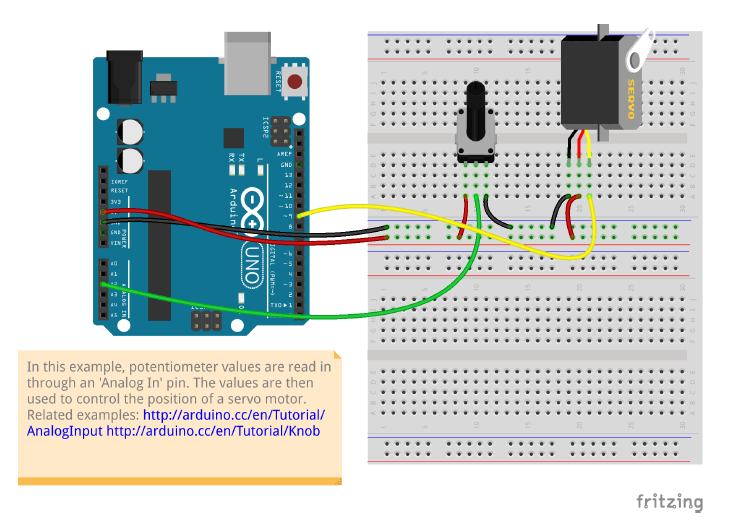
\includegraphics[width=0.6\linewidth]{figures/fritzing.png}
    \caption{Laboratório virtual \textit{Fritzing} exemplo}
    \label{fig:fritzing}
\end{figure}

Um laboratório virtual relativamente recente, apresentado como exemplo na Figura~\ref{fig:wokwi}, embora ainda pouco explorado, que pode constituir uma alternativa bastante interessante ao \textit{Tinkercad}, é o \textit{Wokwi} \cite{wokwi}. Este recurso permite simular diversas placas de desenvolvimento, como o \gls{arduino}, o \gls{ESP32}, o \textit{STM32}, o \gls{RaspberryPI} Pico, bem como uma vasta gama de sensores e actuadores \cite{wokwi}.

\begin{figure}[hbtp]
    \centering
    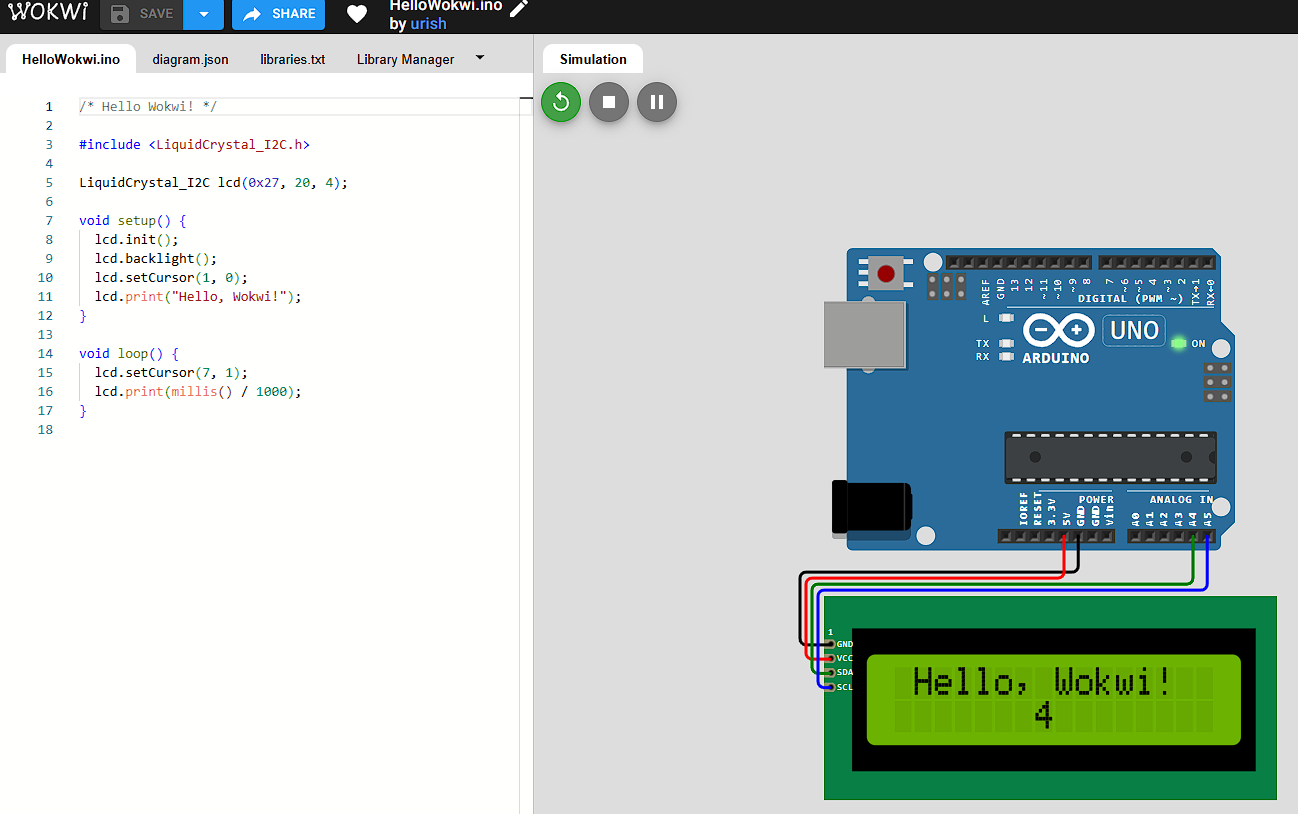
\includegraphics[width=0.6\linewidth]{figures/wokwi.png}
    \caption{Laboratório virtual \textit{Wokwi} exemplo}
    \label{fig:wokwi}
\end{figure}

Os laboratórios virtuais permitem a verificação e o ensaio de circuitos analógicos e digitais complexos. No caso do ensino secundário, por exemplo, plataformas como o \textit{Tinkercad} conseguem reproduzir componentes reais com um grau de precisão adequado a este nível de ensino. As faculdades e universidades de todo o mundo introduzem habitualmente este tipo de \textit{software} de simulação nos seus cursos de engenharia. Uma vez que todos os circuitos são virtuais, os estudantes podem trabalhar e experimentar uma vasta gama de elementos sem o risco de danificar ou destruir equipamento físico. Estes laboratórios virtuais oferecem, assim, um conjunto de oportunidades pedagógicas relevantes, não apenas como substituto, mas também como complemento aos laboratórios reais \cite{WebBrowserSimulators}. 

No caso concreto de uma turma com vinte ou mais alunos, por exemplo, torna-se mais seguro, numa primeira fase, simular circuitos que envolvam componentes como o \textit{TIP120}, o \textit{L293D} ou um microcontrolador como o \gls{arduino}, utilizando plataformas como o \textit{Tinkercad}. Esta abordagem permite aos alunos testar o funcionamento dos circuitos, identificar erros e compreender os princípios de controlo e potência em electrónica básica, antes de avançarem para a montagem física dos projectos. Para além de preservar recursos e reduzir o risco de danos em equipamento real, esta estratégia promove uma aprendizagem mais segura, progressiva e eficaz. Mas as vantagens dos laboratórios virtuais vão muito para além das descritas anteriormente \cite{scheckler, lynch, BlogeMas95, vabtegensVL}. Estes laboratórios oferecem um ambiente seguro para a realização de experiências complexas e potencialmente perigosas, especialmente em fases introdutórias, reduzindo os riscos para estudantes e professores. Permitem ainda que os alunos progridam ao seu próprio ritmo e repitam as experiências tantas vezes quantas forem necessárias, uma vez que estão acessíveis em qualquer momento e a partir de qualquer lugar. Os laboratórios virtuais são, por natureza, mais económicos, de fácil instalação e manutenção. A estas vantagens acresce a vasta disponibilidade de informação, apoio técnico e tutoriais \textit{online} que facilitam a sua integração no processo de ensino-aprendizagem.

No entanto, os laboratórios virtuais também apresentam algumas desvantagens. A principal prende-se com o desfasamento em relação à realidade. Retomando o exemplo anterior - a simulação de circuitos de potência -, o facto de não existirem consequências físicas reais pode induzir uma atitude de desresponsabilização ou falta de cuidado, levando o estudante a assumir que nada de grave poderá acontecer~\cite{POTKONJAK2016309}. Acrescem ainda os constrangimentos relacionados com a constante evolução tecnológica dos sistemas que suportam o laboratório virtual, bem como a necessidade de uma ligação à Internet estável e de qualidade. Quando o laboratório virtual não é utilizado em contexto de sala de aula, tende a reduzir-se a interacção directa entre os alunos e entre estes e os professores, uma vez que a comunicação ocorre sobretudo em ambiente \textit{online}. Além disso, exige-se do aluno um maior grau de autonomia e iniciativa. Há ainda vantagens que, em certos contextos, se podem transformar em desvantagens. Por exemplo, o facto de o aluno poder testar e simular sucessivas vezes sem penalização pode, a longo prazo, reduzir a sua sensibilidade e rigor no manuseamento de componentes reais. Da mesma forma, a imensa quantidade de informação disponível online exige do aluno uma capacidade de selecção crítica e filtragem informada~\cite{POTKONJAK2016309, vabtegensVL, Gherasim, Ghergulescu2019Feb}.

No caso de versão ser remota, as vantagens são semelhantes às de trabalhar com qualquer programa na nuvem:
\begin{itemize}
    \item Não há necessidade de instalar \textit{software} adicional no computador (versão \textit{online});
    \item Desde que a velocidade da Internet seja estável, o simulador pode ser acedido em qualquer lugar;
    \item Os circuitos são guardados e armazenados na nuvem;
    \item É ideal para trabalhos colaborativos e partilha de recursos.
\end{itemize}

\subsubsection{Simuladores - Acesso local e/ou remoto}
Já foi referido na Secção~\ref{sec:questaodeconceitos} que os simuladores são ferramentas que permitem simular o comportamento de sistemas físicos ou electrónicos, sem a necessidade de replicar visualmente os componentes e a disposição dos circuitos. 

Um dos principais simuladores disponíveis gratuitamente, embora com algumas limitações funcionais, e utilizado regularmente em contexto de sala de aula, é o \textit{Multisim Online} \cite{multisim}. Durante os períodos de confinamento, este simulador revelou-se um verdadeiro ``salva-vidas''. Existe também uma versão \textit{premium}, que disponibiliza uma gama mais alargada de recursos \textit{online}, bem como uma versão que pode ser instalada localmente no \acrshort{pc}. O funcionamento destas duas versões é, na práctica, idêntico, sendo que as diferenças situam-se ao nível da \textit{interface} gráfica e, sobretudo, na quantidade de recursos disponível, sendo que na versão local é obviamente muito mais extensa e completa, embora mais desactualizada (Para fins didácticos e educativos a que se propõe, revela-se extremamente eficaz.), como se pode ver na Figura~\ref{fig:multisimlocal} e Figura~\ref{fig:multisimremoto}.

\begin{figure}[hbtp]
    \centering
    \begin{subfigure}[hbtp]{0.48\textwidth}
        \centering
        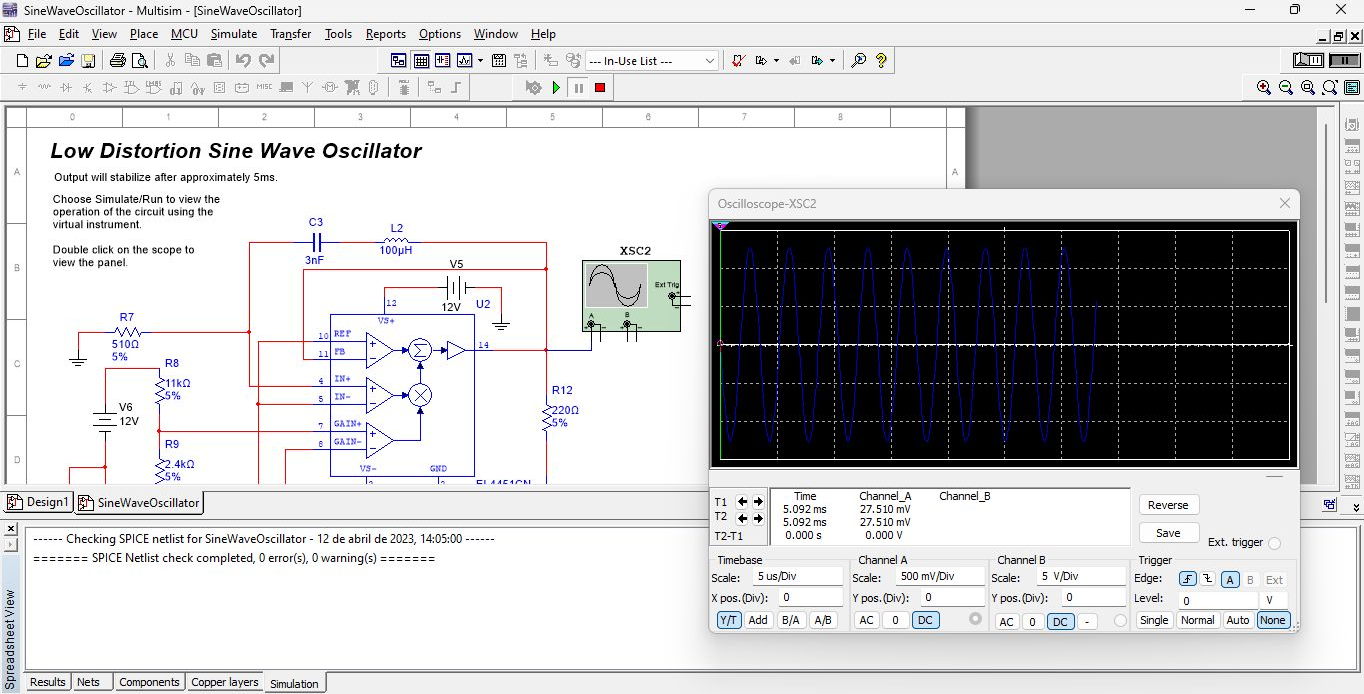
\includegraphics[width=0.9\textwidth]{figures/Multisim_Desktop.png}
        \caption{Local}
        \label{fig:multisimlocal}
    \end{subfigure}
    \begin{subfigure}[hbtp]{0.48\textwidth}
        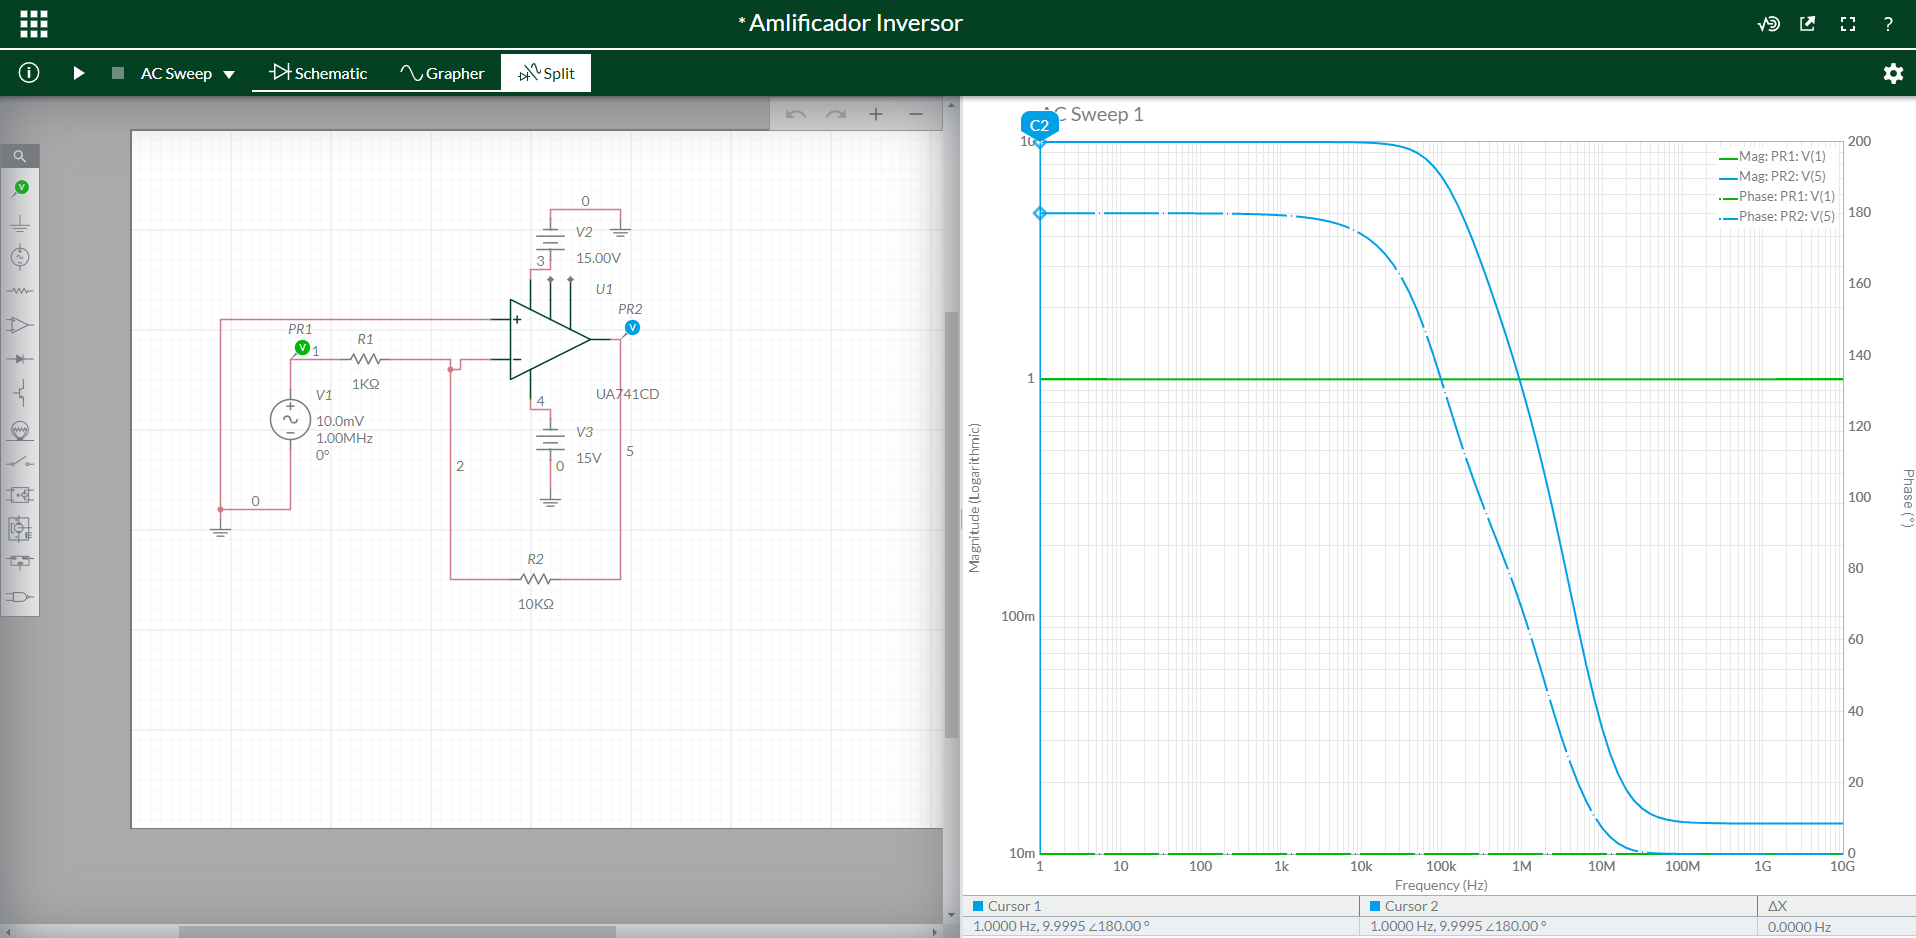
\includegraphics[width=0.9\textwidth]{figures/Multisim_ACsweep.png}
        \caption{Remoto}
        \label{fig:multisimremoto}
    \end{subfigure}
    \caption{Simulador \textit{Multisim}}
    \label{fig:multisimsimulator}
\end{figure}

Ainda assim, para os objectivos de estudo de circuitos simples, no âmbito do currículo do ensino secundário, qualquer das versões se revela adequada. Assim, sempre que for feita referência ao \textit{Multisim} \cite{multisim}, considerar-se-á, salvo indicação em contrário, que a afirmação se aplica a ambas as versões, sem prejuízo da generalidade.

Este \textit{software} integra a simulação virtual \acrfull{spice} padrão da indústria com um ambiente esquemático interactivo para visualizar e analisar instantaneamente o comportamento de circuitos electrónicos. É uma ferramenta poderosa que utiliza modelos matemáticos para simular componentes reais, dispositivos ou circuitos com uma precisão muito boa, através de um navegador \textit{web}. Fornece uma plataforma para ``colmatar'' a lacuna entre a teoria dos manuais e os circuitos reais e também proporciona aos estudantes uma boa plataforma para experiências abrangentes e inovadoras \cite{multisim}. Além disso, dispondo de poderosas funcionalidades de aprendizagem e integração de \textit{hardware} de laboratório, o \textit{Multisim} ensina aos alunos conceitos fundamentais de electrónica analógica, digital e de potência presentes em todo o currículo de engenharia e ciências~\cite{ImportantSimSoftware}.

Tomando novamente o exemplo de uma turma com vinte ou mais alunos, torna-se mais seguro simular circuitos de potência envolvendo componentes com \gls{triac}s, \gls{diac}s ou \gls{scr}s. Além disso, a possibilidade de simular circuitos complexos, como amplificadores operacionais, circuitos digitais e sistemas de controlo, torna o \textit{Multisim} uma ferramenta valiosa para a compreensão dos princípios fundamentais da electrónica.

Citando Heying, Kejie e Li, (2010), ``(\ldots) podemos concluir que a criação de uma plataforma de simulação virtual através do \textit{Multisim} num computador permite construir facilmente todo o tipo de circuitos. (\ldots) Seguem-se os comentários de alguns alunos:''
\begin{itemize}
    \item ``O ensino experimental utilizando o \textit{Multisim} é uma boa abordagem para me ajudar a compreender as matérias;''
    \item ``Gostei de trabalhar na plataforma de simulação virtual \textit{Multisim}'';
    \item ``A simulação \textit{Multisim} ajudou-me a compreender melhor as experiências.''
\end{itemize}

Os mesmos autores concluem que: ``O laboratório virtual [\textit{Multisim}] desempenha um papel muito importante na atualização do método de ensino experimental, na melhoria da qualidade do ensino dos cursos em circuito e na otimização do efeito do ensino.'' \cite{heying}.

Outro simulador, representado como exemplo na Figura~\ref{fig:falstad}, e amplamente utilizado em contexto de sala de aula, foi criado e desenvolvido por Paul Falstad em 1985, estando disponível em www.falstad.com \cite{falstad}. Trata-se de um simulador livre e de código aberto \cite{falstadlicenca}, que funciona directamente num navegador \textit{web} sob a forma de uma \textit{Java Applet}. A sua importância advém, em grande parte, da facilidade de interacção e da simplicidade com que representa circuitos eléctricos — aspectos particularmente relevantes na produção de recursos multimédia nas áreas da Electrónica e da Electricidade\footnote{Para maior rigor, importa referir que este recurso não se limita aos circuitos electrónicos, estando igualmente ligado a outras áreas da ciência, como a termodinâmica, a mecânica quântica, o processamento de sinal, entre outras \cite{falstadcompleto}.}. Além disso, o simulador \textit{Falstad} tem vindo a ser desenvolvido como uma aplicação de Internet há vários anos. De acordo com da Silva et al. (2011) \cite{RemoteTeachingElectricalCircuits}, citados por \textit{Falstad} (2024) \cite{falstad}, este simulador tem demonstrado versatilidade e aplicabilidade no ensino à distância.

O principal constrangimento prende-se com a ausência de parametrização avançada e de um modelo matemático robusto, o que faz com que este simulador não seja adequado para aplicações de engenharia profissional. No entanto, para fins didácticos e educativos, revela-se extremamente eficaz.

Por exemplo, como se pode observar na Figura~\ref{fig:falstad}, destacam-se as seguintes funcionalidades:

\begin{itemize}
    \item Os pontos amarelos animados representam a corrente eléctrica, cujo movimento demonstra o fluxo de cargas em ``tempo real'';
    \item A cor do fio varia entre verde e vermelho, consoante a direcção da corrente;
    \item Os componentes apresentam diferentes níveis de tensão;
    \item As formas de onda podem ser visualizadas directamente no circuito;
    \item É possível representar e controlar diferentes tipos de interruptores (por exemplo, para variar a frequência ou a tensão), o que permite ao utilizador observar fenómenos transitórios;
    \item A velocidade da simulação, bem como a intensidade da corrente, podem ser ajustadas.
\end{itemize}

Estas funcionalidades tornam o simulador \textit{Falstad} uma ferramenta didáctica particularmente útil para introduzir conceitos fundamentais da electrónica, como corrente, tensão, formas de onda e comportamento dinâmico de circuitos. A sua \textit{interface} visual e interactiva contribui para uma melhor compreensão dos fenómenos eléctricos, mesmo por parte de alunos com conhecimentos ainda iniciais. Embora limitado em termos de precisão e análise avançada, este simulador permite visualizar, de forma intuitiva e acessível, muitos dos princípios que são abordados nas aulas teóricas, servindo como uma excelente ponte entre a teoria e a práctica, sobretudo em ambientes com recursos laboratoriais físicos reduzidos.

\subsubsection{Laboratório remoto}
\label{sec: remotelaboratory}
Alguns dos constrangimentos associados aos laboratórios reais já foram abordados ao longo deste capítulo. Apesar do seu inegável valor pedagógico — sobretudo pela possibilidade de os alunos interagirem com recursos físicos e concretos — a sua implementação levanta vários desafios. No ensino secundário e superior, garantir o acesso generalizado a estes recursos nem sempre é viável. Por um lado, há limitações financeiras significativas para manter laboratórios devidamente equipados; por outro, torna-se muitas vezes incomportável assegurar condições para que todos os alunos realizem experiências em simultâneo, especialmente em turmas numerosas. No ensino superior, onde os estudantes são, pelo menos teoricamente, mais autónomos do que no ensino secundário, o principal obstáculo prende-se com a disponibilidade dos laboratórios fora do horário das aulas presenciais.

Numa época em que a tecnologia é cada vez mais encarada como um facilitador no processo de ensino/aprendizagem, a utilização de laboratórios remotos é cada vez mais comum e generalizada \cite{RemoteLabsImpactVISIR}. Além disso, os laboratórios remotos apresentam algumas vantagens em relação aos laboratórios reais e mesmo aos simuladores, tais como: flexibilidade, acessibilidade, disponibilidade e segurança~\cite{RemoteLabsImpactVISIR}. Estes tipos de laboratórios - que incluem, por exemplo, o \acrshort{visir} ou o \textit{LabsLand}~\cite{labsland} - permitem que professores/investigadores e alunos acedam a equipamentos e/ou computadores através da Internet para realizar experiências e tarefas laboratoriais sem estarem no espaço físico dos laboratórios~\cite{ExperiencesRemoteLab}.

Num laboratório remoto, a interacção tem lugar à distância com a ajuda da infraestrutura remota. Esta é uma nova camada que se situa entre o utilizador e o equipamento do laboratório. É responsável pela transmissão das acções do utilizador e pela recepção da informação sensorial do equipamento.
Várias investigações mostram que os estudantes podem efetivamente aprender com a utilização de laboratórios remotos e também de laboratórios virtuais, obviamente se estiverem empenhados no que estão a estudar \cite{RemoteLabsImpactVISIR}. Se se aplicar os conceitos abordados na Secção~\ref{sec:questaodeconceitos}, o \acrshort{visir} pode ser considerado um laboratório remoto virtual, já que a \textit{interface} gráfica tenta replicar, visual e funcionalmente, um ambiente laboratoreal real, tal como representado na Figura~\ref{fig:exemplo_visir}. 

\begin{figure}[hbtp]
    \centering
    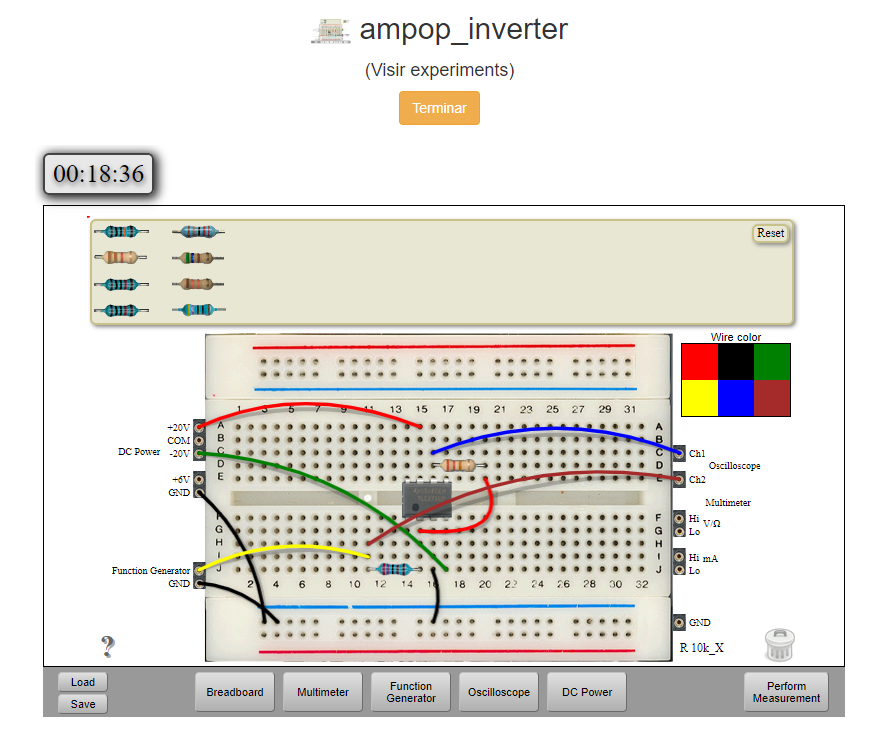
\includegraphics[width=0.4\linewidth]{figures/visir_sch.png}
    \caption{Exemplo \textit{\acrshort{visir}}}
    \label{fig:exemplo_visir}
\end{figure}

De acordo com Viegas \textit{et al.} (2018) \cite{ImpactRemoteLabTeachingPractices}, que citam Brinson (2015) \cite{BRINSON2015218} e Corter \textit{et al.} (2011) \cite{CORTER20112054}, os resultados obtidos com simuladores e laboratórios remotos podem ser considerados semelhantes - ou mesmo superiores - aos dos laboratórios práticos reais. No entanto, uma abordagem à aprendizagem laboratorial que utilize uma combinação de laboratórios práticos, simulações e procedimentos de laboratórios remotos parece ser a forma mais eficaz de aprendizagem, tirando partido dos benefícios dos três \cite{BRINSON2015218}. Esta mesma conclusão foi obtida por de Mel e Samaranayaka (2017) \cite{deMel}, no estudo intitulado ``\textit{Extending the boundaries of remote laboratory by providing hands on experience}''. Citando os autores: ``(\ldots) os estudantes estão disponíveis a usar o laboratório remoto juntamente com o real (\ldots)'', mas ``(\ldots) não aconselham a total substituição (\ldots)''. O estudo conclui, ainda, que não há grande diferença entre o laboratório real e remoto, sendo que os conhecimentos adquiridos são (praticamente) os mesmos.

Podem ser considerados outros estudos que, por exemplo, comparem laboratórios reais (práticos) e simulados, laboratórios reais e virtuais. De facto, Corter \textit{et al.} (2007) \cite{StudyRemoteHandsonSimulatedLabs}, no seu estudo intitulado ``\textit{Constructing reality: A study of remote, hands-on, and simulated laboratories}'' concluem que ``(\ldots) os laboratórios remotos e simulados podem ser pelo menos tão eficazes como os laboratórios práticos tradicionais no ensino de conceitos específicos da disciplina''. Outro estudo feito por Kocijancic e O'Sullivan (2004) \cite{RealorVirtualDilema}, intitulado ``\textit{Real or virtual laboratories in science teaching - is this actually a dilemma?}'', conclui que ``(\ldots) não se trata de saber se é melhor utilizar experiências reais ou laboratórios virtuais no ensino das ciências, uma vez que ambas as abordagens, utilizadas de forma complementar, podem contribuir para uma aprendizagem activa mais eficaz.''. Tsihouridis \textit{et al.} (2019), concluem também que ``não há um vencedor final nesta controvérsia intemporal entre os dois ambientes de laboratório experimental, de acordo com a nossa investigação.'' \cite{controversy}.

Ainda que os estudos apontem para a complementaridade entre laboratórios reais e remotos (virtuais e simuladores), é relevante compreender os factores que explicam o crescimento acentuado deste tipo de laboratórios em contextos de ensino. Segundo Nafalski et al. (2010) \cite{ExperiencesRemoteLaboratories}, com base em Auer e Gravier (2009) \cite{ThemMnyfacesRemotLab}, este crescimento está relacionado com:

\begin{itemize}
    \item A crescente complexidade das tarefas de engenharia;
    \item O equipamento cada vez mais especializado e dispendioso, as ferramentas de software e os simuladores necessários;
    \item A necessidade de utilizar equipamentos e ferramentas de \textit{software}/simuladores dispendiosos em projectos com prazos curtos (como os apresentados em \cite{ExperiencesRemoteLab});
    \item A aplicação de equipamentos de alta tecnologia necessários em pequenas e médias empresas;
    \item A necessidade de pessoal altamente qualificado para controlar os novos equipamentos;
    \item As exigências da globalização e da divisão do trabalho.
\end{itemize}

No entanto, segundo Fan \textit{et al.} (2021) \cite{EvaluationRemoteVirtualE-Learning}, a integração de laboratórios remotos com a \gls{industria40} - tema já abordado no Capítulo~\ref{Capítulo1} - apresenta várias vantagens. Esta perspectiva é sustentada por vários autores citados no seu estudo, incluindo Tawfik \textit{et al.} (2016) \cite{RemoteLabsImpactVISIR}, Chen \textit{et al.} (2010) \cite{DevelopingVirtualAndRemoteUndergraduate} e Simão \textit{et al.} (2014) \cite{RemoteLabsDevelopingCountries} que identificam os seguintes benefícios:
\begin{itemize}
    \item Os estudantes podem fazer os exercícios da disciplina ao seu próprio ritmo e de acordo com o seu nível de interesse;
    \item A quantidade de tempo (muitas vezes horas extraordinárias) que os professores têm de despender na preparação e ensino dos laboratórios pode ser reduzida;
    \item Podem ser efectuadas várias experiências utilizando a mesma configuração;
    \item Os laboratórios remotos permitem o acesso de um maior número de utilizadores, o que significa que a sua instalação acaba por ser mais barata do que a dos laboratórios físicos;
    \item Os laboratórios remotos estão acessíveis 24 horas por dia, 7 dias por semana;
    \item Os laboratórios remotos podem ajudar a reforçar o trabalho autónomo dos alunos;
    \item Os laboratórios remotos são mais seguros, tanto para o utilizador como para o equipamento ou software, uma vez que estão fisicamente separados e são orientados para a tecnologia.
\end{itemize}

Embora os laboratórios remotos ofereçam muitas vantagens, como as descritas em cima, é importante estar ciente das suas desvantagens (muitas delas comuns com as descritas para os laboratórios virtuais). A falta de interacção física directa, a dependência da ligação com a Internet, os desafios técnicos e de manutenção, a experiência de aprendizagem menos imersiva e a limitação da interacção com colegas e professores são pontos críticos que devem ser considerados ao implementar esses laboratórios. No entanto, a principal desvantagem prende-se com a complexidade da sua implementação. Como os laboratórios remotos seguem uma arquitectura cliente-servidor, além do servidor é ainda necessário ter em conta a questão do \textit{hardware} e a sua integração com o \textit{software} que pode, ou não, ser proprietário. Há ainda a questão essencial da forma como os utilizadores acedem ao laboratório. Isto levanta problemas de largura de banda, que restringe o número de utilizadores que podem aceder simultaneamente ao laboratório remoto \cite{HERADIO20161}.

Existem muitos tipos de laboratórios nos mais diversos campos da ciência - como a Física, Electrónica, Robótica ou Química - e com distintas arquitecturas de \textit{hardware} e \textit{software}. Entre os laboratórios remotos atualmente em funcionamento, e que abrangem as áreas \acrshort{stem}, destacam-se os seguintes:
\begin{itemize}
    \item A Universidade de \textit{Deusto}, em Bilbao tem disponível uma conjunto de laboratórios remotos, que inclui o \acrshort{visir}, o comando de um robô através de um \gls{arduino} ou a programação de uma \acrfull{fpga};
          %\textit{WebLab-Deusto} - O \textit{WebLab-Deusto} é uma iniciativa da Universidade de Deusto com o objectivo de aumentar a aprendizagem experimental através da utilização e desenvolvimento de laboratórios remotos
    \item \textit{iSES}\footnote{\url{https://www.ises.info/index.php/en/systemises/sdkisesstudio}} - tem várias experiências remotas que abrangem diversas áreas da ciências, como Física, Electrónica, Radioactividade, Electromagnetismo, etc.
    \item \textit{OpenSTEM}\footnote{\url{https://learn5.open.ac.uk/}} - estes laboratórios têm uma colecção de experiências abrangendo áreas científicas que vão desde a saúde, engenharia ou observatórios;
    \item \textit{Remote-LAB GymKT}\footnote{\url{http://remote-lab.fyzika.net/}} - Várias experiências que vão desde o controlo de um braço robótico através de um \gls{arduino} até experiências no campo da Física e da Electrónica;
\end{itemize}

Em síntese, os laboratórios remotos não devem ser vistos apenas como uma versão reduzida dos laboratórios reais (práticos), mas como uma abordagem distinta, com pontos fortes e limitações próprias, que oferece oportunidades de aprendizagem únicas, não proporcionadas pelas metodologias tradicionais. Quando integrados de forma complementar com laboratórios físicos e simulações, permitem explorar o melhor de cada abordagem.
Com base nos estudos apresentados nos parágrafos anteriores, pode afirmar-se com segurança que os laboratórios remotos constituem uma alternativa viável - e, em muitos casos, vantajosa - face aos laboratórios convencionais, sobretudo pela sua maior acessibilidade e pela redução de custos operacionais. Os resultados de aprendizagem não parecem ser significativamente afectados pela sua utilização. De facto, algumas universidades já os começaram a integrar nas suas sessões práticas~\cite{VISIREngineeringPractices}.

\subsubsection{VISIR - Virtual Instrument Systems in Reality}
\label{sec:visir}
No contexto desta dissertação, importa, no entanto, abordar o caso particular do \acrshort{visir}. De facto, este laboratório remoto esteve na génese da criação do \acrshort{lare} e encontra-se actualmente disponível no \acrshort{isep}, conforme ilustrado na Figura~\ref{fig:visirISEP}.
\begin{figure}[hbtp]
    \centering
    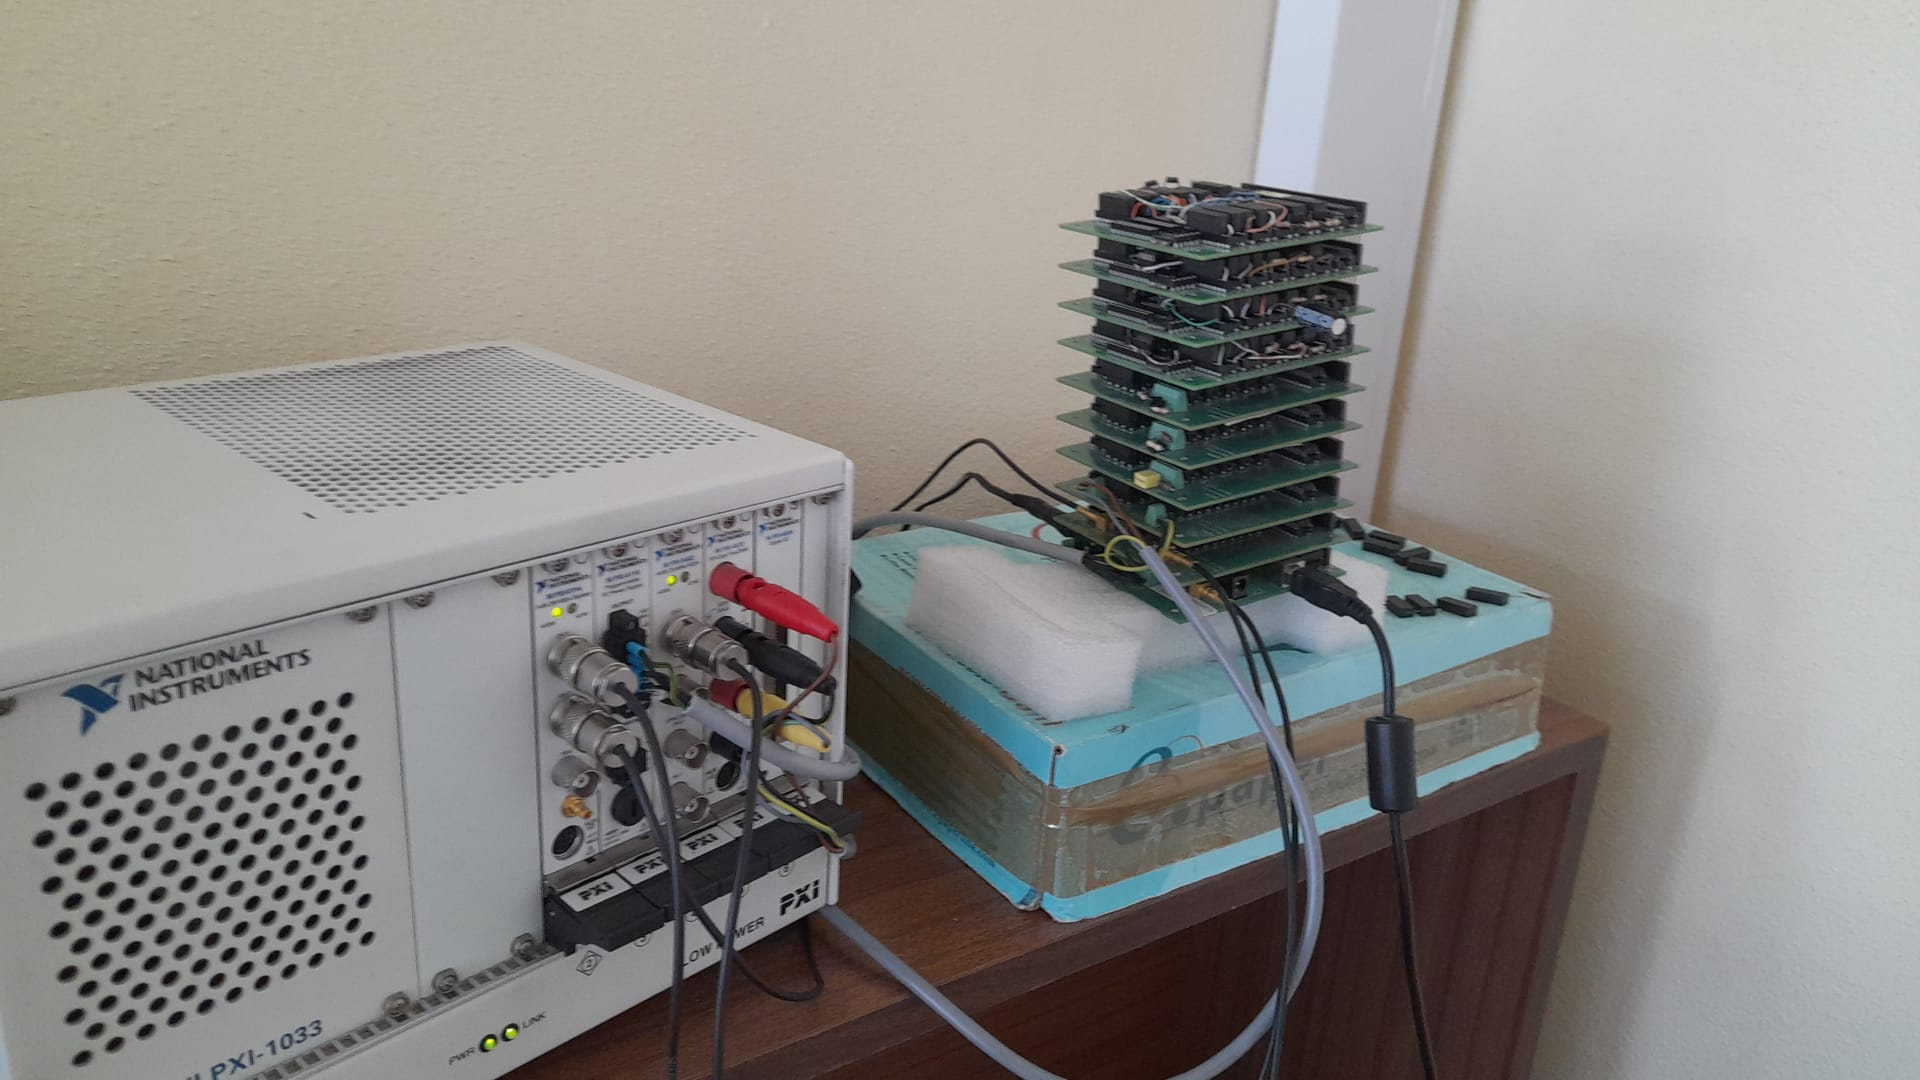
\includegraphics[width=0.75\textwidth]{figures/visirISEP.jpeg}
    \caption{\acrshort{visir} no \acrshort{isep}}
    \label{fig:visirISEP}
\end{figure}

O \acrshort{visir} é um laboratório remoto para concepção, ligação e medição de circuitos electrónicos. O sistema \acrshort{visir} foi desenvolvido no \acrfull{bth}, \textit{Karlskrona}, Suécia, em 1999, e as suas funcionalidades e comunidade de utilizadores têm vindo a crescer desde então \cite{RemoteLabsImpactVISIR}. O projecto foi lançado no final de 2006 em conjunto com a \acrshort{ni}, nos \acrshort{eua}, (como fornecedor de instrumentos) e a \textit{Axiom EduTECH} na Suécia (como fornecedor de educação, \textit{software} técnico e serviços de engenharia para análise de ruído e vibrações). Foi apoiado financeiramente pela \acrshort{bth} e pela Agência Governamental Sueca para os Sistemas de Inovação (VINNOVA)~\cite{VISIRExperiencesChallenges}. Este sistema oferece aos estudantes a oportunidade de utilizarem recursos experimentais 24 horas por dia, 7 dias por semana, sem um aumento significativo no custo por estudante. Com mais tempo dedicado a estas experiências, os estudantes tornam-se verdadeiros ''experimentadores``, capazes de criar bens e serviços que satisfaçam os requisitos de uma sociedade sustentável. Desta forma, o \acrshort{visir} não só melhora a aprendizagem, mas também contribui para a formação de profissionais comprometidos com o desenvolvimento sustentável \cite{OpenLabs77:online}.

Em 2018, tal como referido no artigo ``\textit{PILAR: a Federation of VISIR Remote Laboratory Systems for Educational Open Activities}'' \cite{PILARFederationVISIR}, o \acrshort{visir} já tinha sido implementado em 8 Instituições de Ensino Superior diferentes, situados em 6 países, incluindo o \acrshort{isep} (Portugal). No mesmo ano, segundo a mesma publicação, foram instalados novos sistemas em várias instituições da América do Sul. O \textit{software} do \acrshort{visir} é lançado sob uma licença GNU GPL. O conceito subjacente a este consiste em acrescentar uma opção de operação remota aos laboratórios de ensino tradicionais para os tornar mais acessíveis, independentemente dos alunos estarem no \textit{campus} ou principalmente fora do \textit{campus}~\cite{TheVISIRproject}.

A arquitectura, do \acrshort{visir} pode ser dividida em quatro partes, tal como referido em \cite{tawfikexperiences} e como se pode ver na Figura~\ref{fig:platvisir} esta arquitectura inclui:
\begin{itemize}
    \item \textit{Equipment  Server} - Compreende todo o equipamento do \acrshort{visir} (módulos e \textit{chassis}): as placas \acrfull{pxi} e instrumentação (que estão ligadas à matriz de relés) controlados através do \acrshort{labview};
    \item \textit{Measurement Server} - Trata-se de um servidor escrito em Visual C++ para a \textit{Microsoft}. É programado por ficheiros ``max list'' que contêm os valores máximos dos componentes e ajustes dos instrumentos para cada experiência e servem para evitar a concepção de circuitos perigosos e proteger os instrumentos;
    \item \textit{Web Server} - Aloja a \textit{interface Web} do \acrshort{visir} e foi concebida em \textit{Apache} com uma base de dados em \textit{MySQL};
    \item \textit{Web Interface}, Figura \ref{fig:protoboadrvisir} - É o \textit{site} do \acrshort{visir} e foi escrito em PHP, com o cliente de experiências integrado escrito em \textit{Flash}.
\end{itemize}

\begin{figure}[hbtp]
    \centering
    \begin{subfigure}[hbtp]{0.48\textwidth}
        \centering
        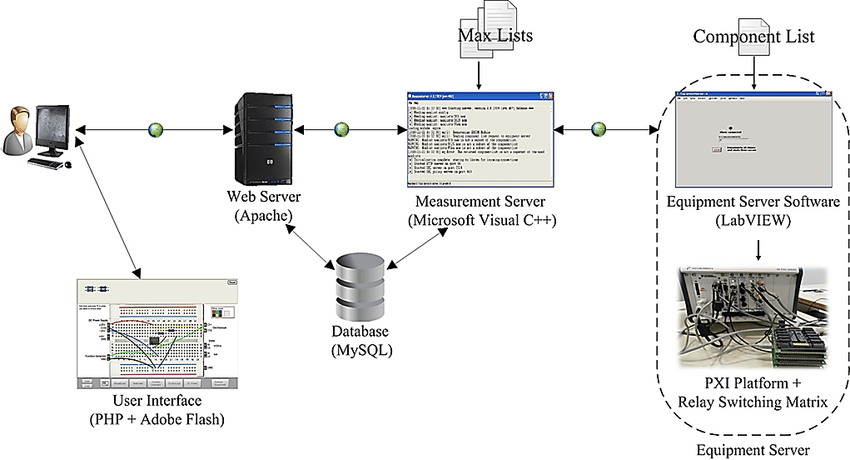
\includegraphics[width=0.9\textwidth]{figures/arquitectura_VISIR.png}
        \caption{Plataforma \acrshort{visir} \cite{tawfikexperiences}}
        \label{fig:platvisir}
    \end{subfigure}
    \begin{subfigure}[hbtp]{0.48\textwidth}
        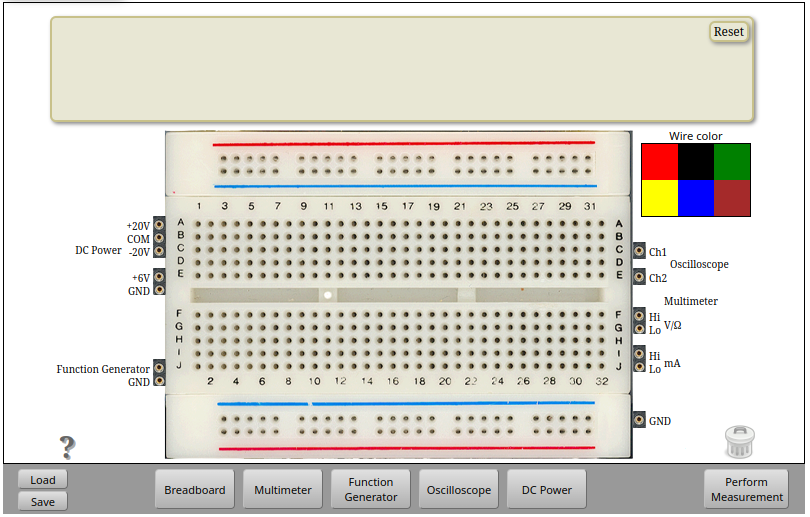
\includegraphics[width=0.9\textwidth]{figures/protboard_visir.png}
        \caption{\textit{Protoboard} \acrshort{visir}}
        \label{fig:protoboadrvisir}
    \end{subfigure}
    \caption{Arquitectura do \acrshort{visir}}
    \label{fig:arquitecturavisir}
\end{figure}

O \textit{chassis} PXI-1033 \cite{PXI-1033}, Figura~\ref{fig:PXI-1033}, é um controlador integrado com 5 \textit{slots} que foi concebida para aplicações de controlo remoto. Naturalmente, este dispositivo exige um \textit{interface} para \acrshort{pc}, que, neste caso, é feito através do \acrshort{labview}.

\begin{figure}[hbtp]
    \centering
    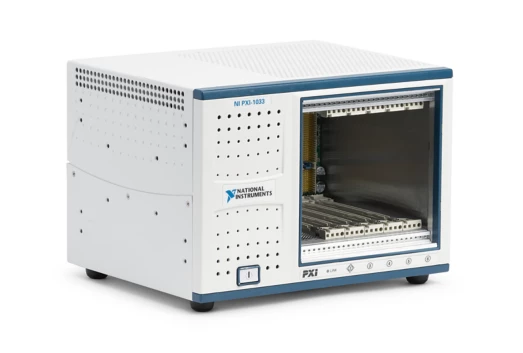
\includegraphics[width=0.4\textwidth]{figures/PXI-1033.png}
    \caption{\textit{Chassis} PXI-1033 \cite{PXI-1033}}
    \label{fig:PXI-1033}
\end{figure}

Existem várias possibilidades de integração de módulos na PXI-1033, nomeadamente os que compõem o sistema \acrshort{visir}. Estes módulos podem variar consoante a configuração pretendida, estando disponíveis diversas opções adicionais no site oficial da National Instruments\footnote{\url{https://www.ni.com/en-us}}. No caso do \acrshort{visir}, os módulos utilizados são os seguintes:
\begin{itemize}
    \item Osciloscópio, PXI-5114, \SI{12}{\MHz}, 250 MS/s, 8-Bit, Figura \ref{fig:PXI-5114}
          \begin{figure}[hbtp]
              \centering
              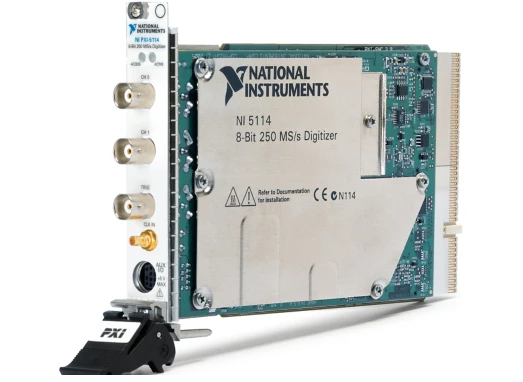
\includegraphics[width=0.4\textwidth]{figures/PXI-5114.png}
              \caption{Osciloscópio PXI-5114 \cite{PXI-5114}}
              \label{fig:PXI-5114}
          \end{figure}
    \item Gerador de sinal, PXI-5402, \SI{10}{\MHz} \textit{Bandwidth}, 1-\textit{Channel}, 14-Bit, Figura \ref{fig:PXI-5402}
          \begin{figure}[hbtp]
              \centering
              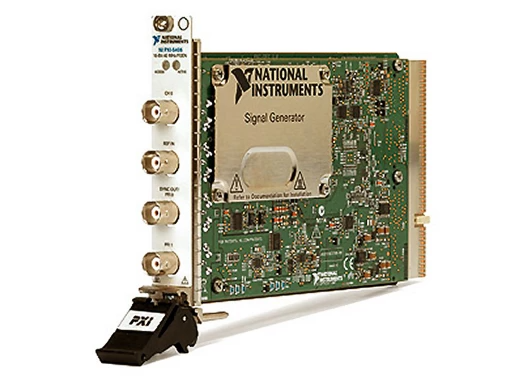
\includegraphics[width=0.4\textwidth]{figures/PXI-5402.png}
              \caption{Gerador de sinal PXI-5402 \cite{PXI-5402}}
              \label{fig:PXI-5402}
          \end{figure}
    \item Multímetro Digital, \(6^{1/2} \)Digitos, \(\pm\)\SI{300}{\volt}, \textit{Onboard} 1.8 MS/s Digitalizador isolado, suporte para medições de indutâncias e capacitâncias, Figura \ref{fig:PXI-4072};
          \begin{figure}[hbtp]
              \centering
              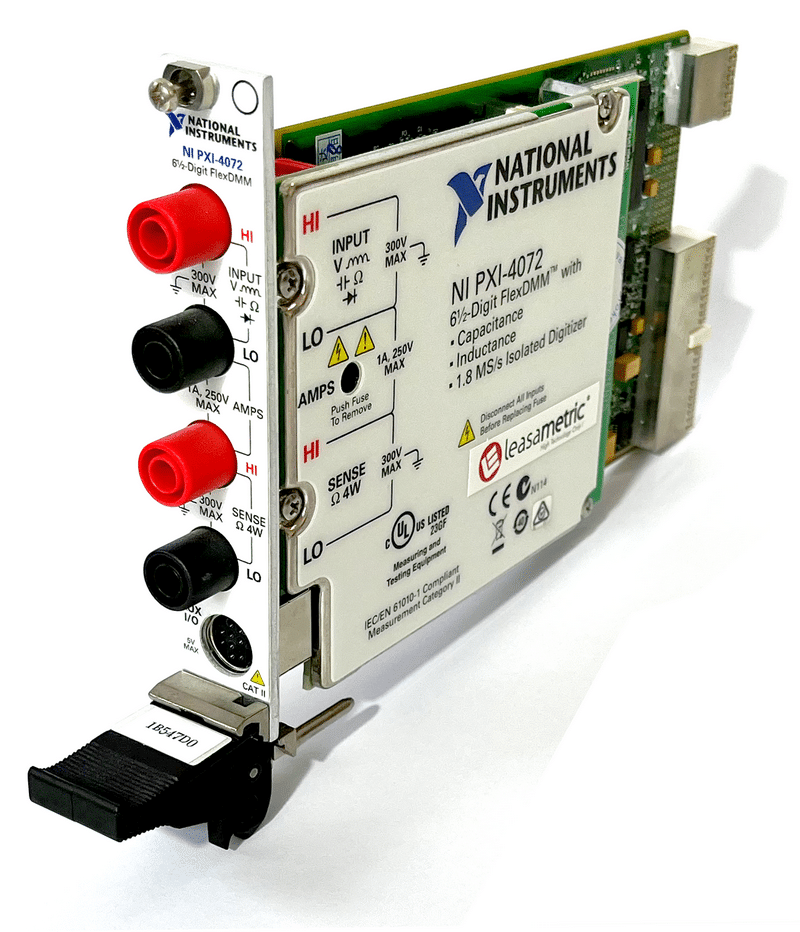
\includegraphics[width=0.3\textwidth]{figures/PXI-4072.png}
              \caption{Multímetro Digital PXI-4072 \cite{PXI-4072}}
              \label{fig:PXI-4072}
          \end{figure}
    \item Fonte de tensão programável, 3 canais, corrente de saída máxima de \SI{1}{\ampere}, gama de tensão de saída analógica: -\SI{20}{\volt} a \SI{20}{\volt}, Figura {\ref{fig:PXI-4110}}.
          \begin{figure}[hbtp]
              \centering
              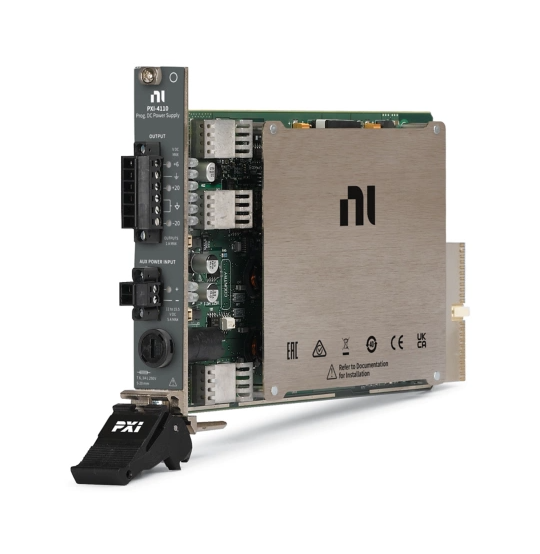
\includegraphics[width=0.4\textwidth]{figures/PXI-4110.png}
              \caption{Fonte de tensão PXI-4110 \cite{PXI-4110}}
              \label{fig:PXI-4110}
          \end{figure}
\end{itemize}

O \acrshort{visir} possuí uma \acrfull{mcr} concebida no \acrshort{bth} especialmente para o uso em experiências electrónicas em laboratórios remotos tal como ser visto na Figura~\ref{fig:matrizvisir}. Esta matriz é constituída por quatro placas PC/104\footnote{\url{https://pc104.org/}} (de baixo para cima): fontes de tensão, multímetro digital, osciloscópio e a placa de topo permite configurar os componentes. A matriz é controlada por uma \acrfull{pic}, PIC18F4550 \cite{PIC18F4516datasheet}, montada na placa de alimentação (fontes de tensão) e comunica com um \acrshort{pc}, via \acrshort{usb}, e com os controladores das outras placas através das \acrshort{pic}s, PIC16F767 \cite{PIC16F7675datasheet}, via \acrfull{i2c}, montadas em cada placa \cite{matriz}.

\begin{figure}[hbtp]
    \centering
    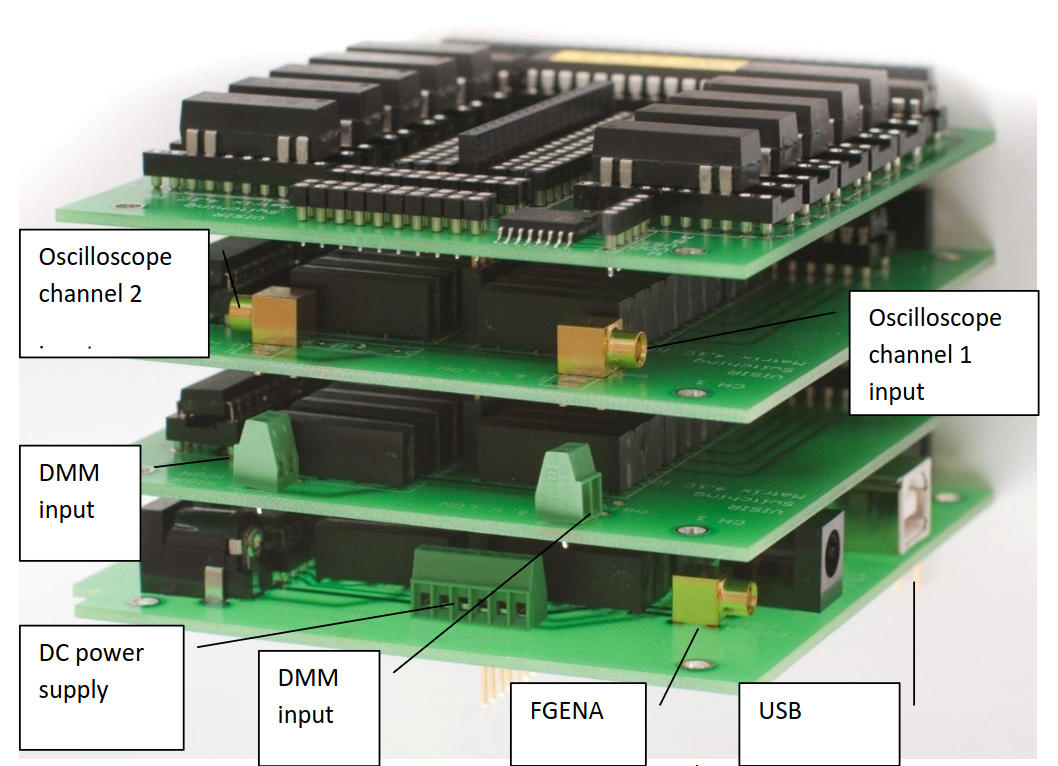
\includegraphics[width=0.4\textwidth]{figures/matriz.png}
    \caption{Matriz \acrshort{visir}\cite{matriz}}
    \label{fig:matrizvisir}
\end{figure}

Segundo Tawfik et al. (2012) \cite{tawfikexperiences} e Tawfik et al. (2013) \cite{tawfikvisir}, seis universidades já tinham implementado o \acrshort{visir}. No entanto, Pereira et al. (2017) referem que o \acrshort{visir} estava presente em 12 instituições e sete países \cite{pereira}.

Levanta-se, então, uma questão: Como fazer a integração de todos os laboratórios remotos de forma a aproveitar os recursos e potenciar o trabalho colaborativo?

\paragraph{PILAR}
O projecto \textbf{\acrfull{pilar}} \textit{Erasums+}, foi iniciado em 2016 tendo terminado em 2019 e tinha como objectivo a criação de uma Federação de cinco nós \acrshort{visir} existentes, partilhando experiências, capacidade e recursos entre as diversas instituições e permitir o acesso ao laboratório remoto \acrshort{visir}, através do consórcio \acrshort{pilar}, a estudantes de outras instituições de ensino \cite{garcia-loro}.

O \acrshort{visir} \acrfull{sig} é organizado para pessoas interessadas em Engenharia \textit{online} ou remota, especialmente na abertura de laboratórios universitários para acesso remoto 24/7. Este projecto foi lançado com o objectivo de divulgar métodos de abertura de laboratórios para acesso remoto,  partilhar ideias, equipamento e material didáctico, bem como de discutir o desenvolvimento da plataforma \acrshort{visir}. Outro dos objectivos é a padronização de bancos de trabalho \textit{online} localizados em universidades de todo o mundo, constituindo laboratórios de rede disponíveis para sessões de laboratório para estudantes dentro e fora do \textit{campus}~\cite{visirsig}.

A missão da Federação \acrshort{visir} é actualizar e alargar o \acrshort{visir} \acrshort{sig}, integrando indivíduos e instituições. O objectivo é fornecer um sistema uniforme, em que os estudantes se possam registar e utilizar os laboratórios federados baseados no \acrshort{visir} e os materiais de aprendizagem de diferentes instituições pertencentes à Federação. Através de um mecanismo comum partilhado, deverá ser possível aceder a cada experiência a partir de um único sistema de gestão da aprendizagem. Os principais objectivos da Federação são \cite{visirfederation}:
\begin{itemize}
    \item Expandir o \acrshort{sig} a instituições;
    \item Conectar todos os nós \acrshort{visir};
    \item Alargar a gama de aplicações;
    \item Melhorar a utilização do \acrshort{visir};
    \item Promover o laboratório remoto \acrshort{visir};
    \item Partilhar materiais de aprendizagem;
    \item Trocar experiências entre os detentores e utilizadores do \acrshort{visir}.
\end{itemize}

Como se viu anteriormente, o \acrshort{visir} funciona numa base de cliente-servidor, o que significa que, se um determinado servidor não estiver disponível, também o laboratório não estará. Neste caso, a Federação permite o redireccionamento dos pedidos dos clientes para um outro nó \acrshort{visir} que esteja disponível \cite{kreiter}.

\chapter{LaRE - Laboratório Remoto Expansível}
\label{Capítulo3}
\begin{flushright}
\textit{``All we have to decide is what to do with the time that is given us.''} \\[0.5em]
--- Gandalf, \textit{The Lord of the Rings: The Fellowship of the Ring}
\end{flushright}

Neste capítulo descreve-se o processo que levou à criação do \acrshort{lare}, a arquitectura de \textit{hardware} e \textit{software}, o motivo das escolhas e a implementação dos circuitos.

\section{Contextualização}
\label{sec:contextualização}
Como já foi referido na Secção \ref{sec:Objectivos} o principal objectivo desta dissertação passa pelo desenvolvimento de um \acrshort{laboratório remoto} para o ensino da electrónica, que visa colmatar (ou resolver) algumas dos limitações que afectam o \acrshort{visir}.

De acordo com a Secção~\ref{sec:visir}, o \textit{software} do \acrshort{visir} foi disponibilizado sob licença GNU GPL. No entanto, o \textit{software} de programação do \textit{firmware} do controlador da matriz, fornecido com o próprio sistema, não é livre, o que significa que não pode ser modificado ou atualizado por terceiros. Acresce ainda que o equipamento associado aos módulos e placas de instrumentação é controlado através do \acrshort{labview}, cujas licenças têm custos anuais que variam entre 523€ e 4300€, conforme a versão adquirida \cite{labviewpricing}.

A criação do \acrshort{laboratório remoto} surge, assim, como resposta prática a estas limitações. Numa fase inicial do desenvolvimento, foram realizados testes preliminares de controlo de relés utilizando um \gls{arduino} Mega, representado na Figura~\ref{fig:arduinomega}, em conjunto com um ambiente de programação simples implementado em \acrshort{labview}.

\begin{figure}[hbtp]
    \centering
    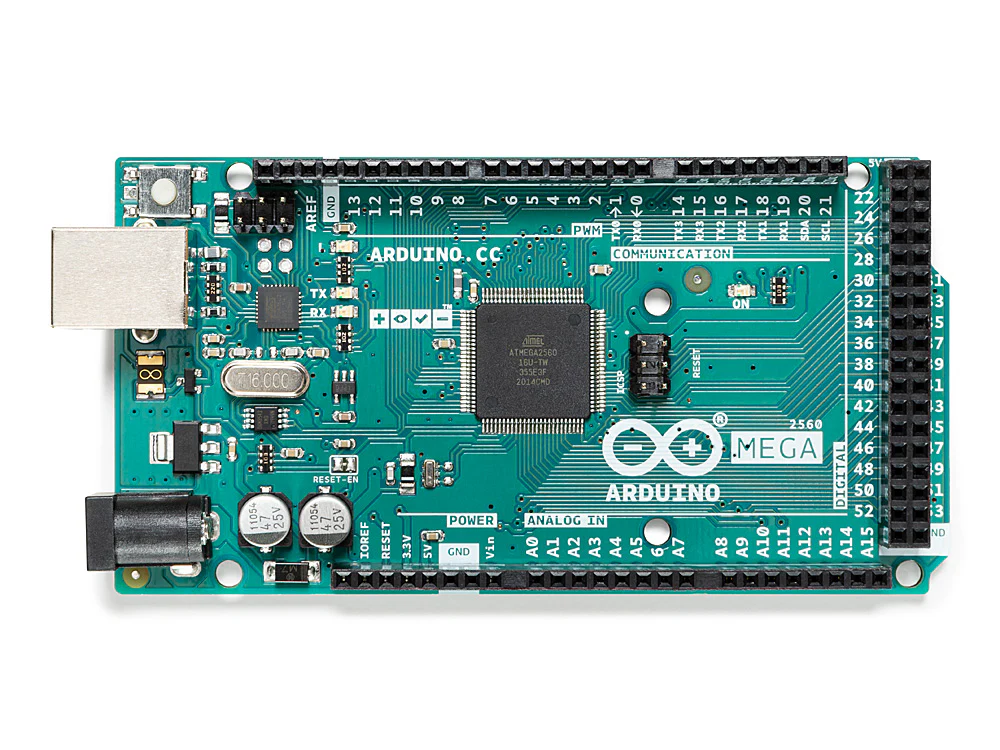
\includegraphics[width=0.4\textwidth]{figures/arduinomega.png}
    \caption{\textit{Arduino} Mega \cite{ArduinoMega}}
    \label{fig:arduinomega}
\end{figure}

No entanto, de forma a ultrapassar o problema levantado pelo elevado preço do \acrshort{labview}, surge um segundo objectivo que se prende com a substituição deste \textit{software} por outro que fosse gratuito e \textit{open source}. A eliminação do \acrshort{labview} implicou a implementação de um servidor. Sendo assim, numa primeira abordagem, foram analisadas algumas opções, tais como: \textit{FastApi}\footnote{\url{https://fastapi.tiangolo.com/}}, \textit{Django}\footnote{\url{https://www.djangoproject.com/}} e \textit{Flask}\footnote{\url{https://flask.palletsprojects.com/en/3.0.x/}}. Estas opções enquadram-se no que se pode chamar \textit{frameworks} ou \textit{micro-frameworks}. Neste caso são todas desenvolvidas para aplicação em \gls{python}.

Uma \textit{micro-framework} é um tipo de \textit{framework} minimalista, que fornece apenas as funcionalidades essenciais para o desenvolvimento de aplicações, sem incluir bibliotecas ou componentes adicionais que não os estritamente necessários. Isso permite a quem desenvolve adicionar apenas as funcionalidades específicas para cada projecto ou aplicação. Daqui resulta um ambiente de desenvolvimento mais leve e flexível \cite{Flask}.
Optou-se, então, pelo \textit{Flask} e as razões da escolha, assim como uma explicação mais detalhada serão apresentadas na Secção \ref{sec:arquitecturasoftware}.

É possível combinar o \gls{arduino} com o \gls{python}, mas isso implicaria uma mudança ao nível do \textit{firmware}, uma tarefa que não é trivial \cite{Arduinopython}. A linguagem nativa do \gls{arduino} é similar ao \textit{C++} e o \textit{firmware} instalado foi projectado para interpretar e executar código escrito nesse tipo de linguagem. De forma mais rigorosa, o uso do \textit{Python} no \gls{arduino} ou em qualquer outro microcontrolador, faz-se através de \textit{MicroPython}, uma implementação simples e eficiente do \gls{python} que inclui um pequeno subconjunto da bibliotecas padrão e é optimizado para funcionar em microcontroladores e em ambientes limitados \cite{MicroPythondefinition}. Quer isto dizer que todas as bibliotecas usadas na programação da aplicação ou projecto têm de ser carregadas para a memória dos microcontroladores. No caso do \gls{arduino} Mega, uma análise ao \textit{datasheet} \cite{megadatasheet} revela que este tem \SI{256}{Kbytes} reservados para o envio de programas e \SI{8}{Kbytes} de memória \textit{SRAM} reservado para variáveis temporárias.
Além destes problemas de memória e uma vez que é necessário que o \gls{arduino} funcione como servidor, foi necessário encontrar uma alternativa mais adequada Arduino Mega, versão apresentada na Figura \ref{fig:arduinomega} não é adequada.

No mercado, existe o \gls{ESP32}, uma alternativa mais poderosa que o \gls{arduino} e com placa de rede sem fios integrada, tal como é apresentado na Figura \ref{fig:ESP32}. No entanto, este microcontrolador sofre dos mesmos problemas de memória que o \gls{arduino} Mega e da utilização do \textit{MicroPython}. Uma análise ao \textit{datasheet} \cite{esp32datasheet} revela que a memória \textit{flash} varia entre os 4-16 \acrlong{mb}. No modelo ''ESP32-DEVKITC-32E``, que estava disponível para este projecto, o valor é de 4 \acrshort{mb} \cite{diferencaspython}. Estas limitações não permitem a implementação de um servidor minimamente robusto usando o \gls{arduino} Mega ou o \gls{ESP32}.

\begin{figure}[hbtp]
    \centering
    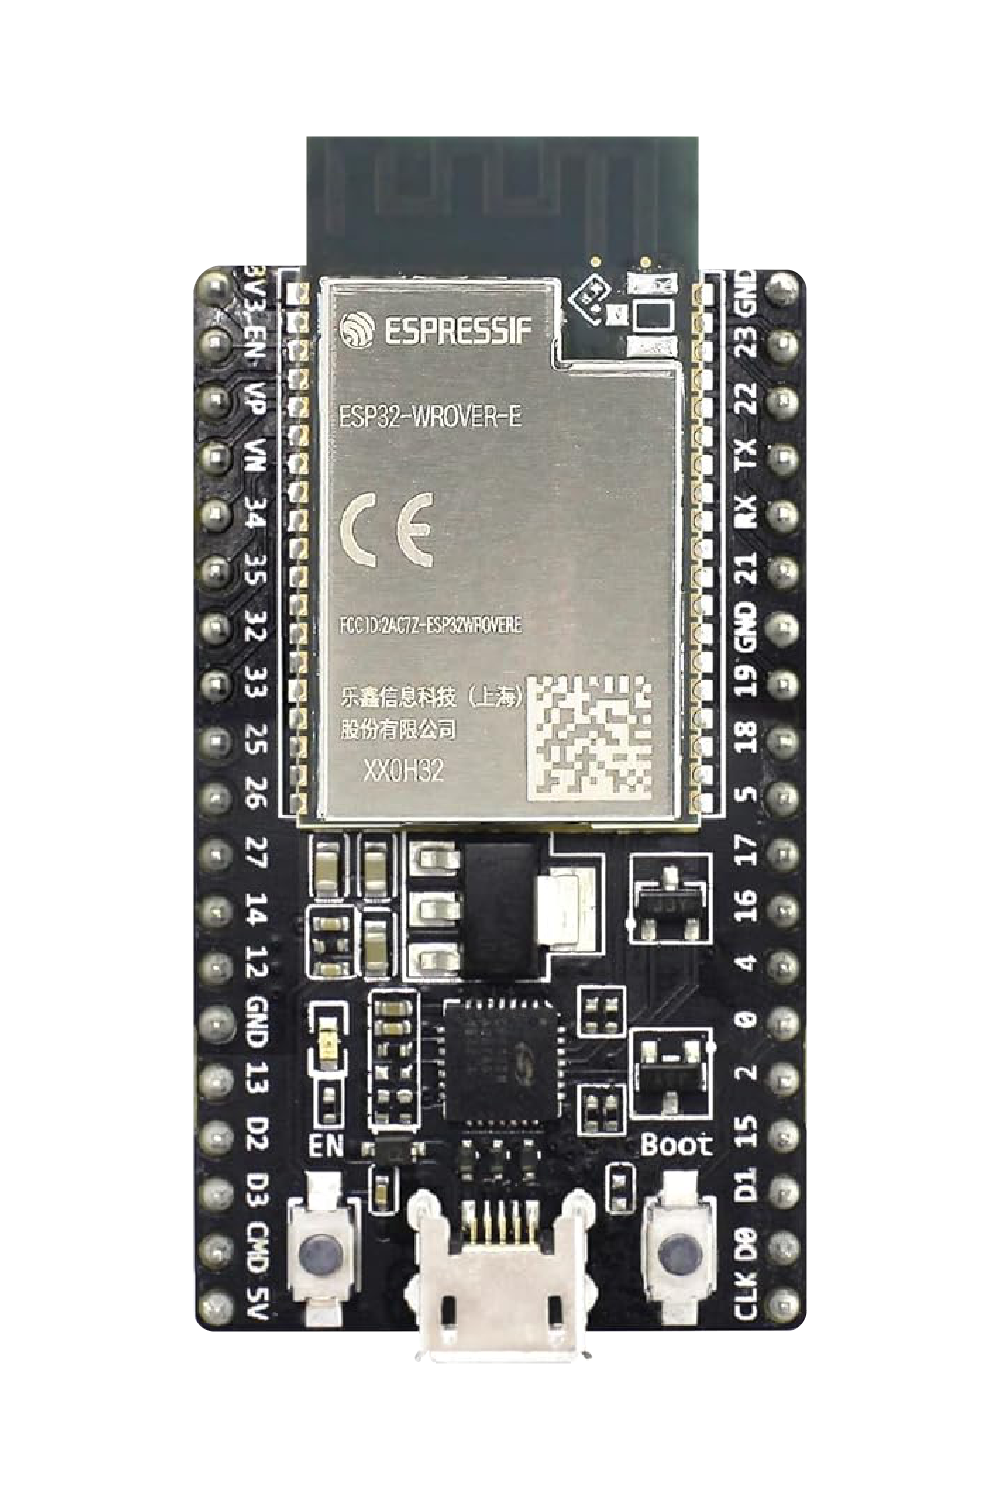
\includegraphics[width=0.4\textwidth]{figures/ESP32-DevKitC_L_0.png}
    \caption{\textit{ESP32} \cite{ESPDevKit}}
    \label{fig:ESP32}
\end{figure}

A opção seguinte recaiu no \gls{RaspberryPI}, versão 5\footnote{Doravante, sempre que for referido \textit{Raspberry Pi}, subentende-se a versão 5.}, que à data da escrita desta dissertação é a versão mais actual, apresentada na Figura \ref{fig:Raspberrypi5}. 

\begin{figure}[hbtp]
    \centering
    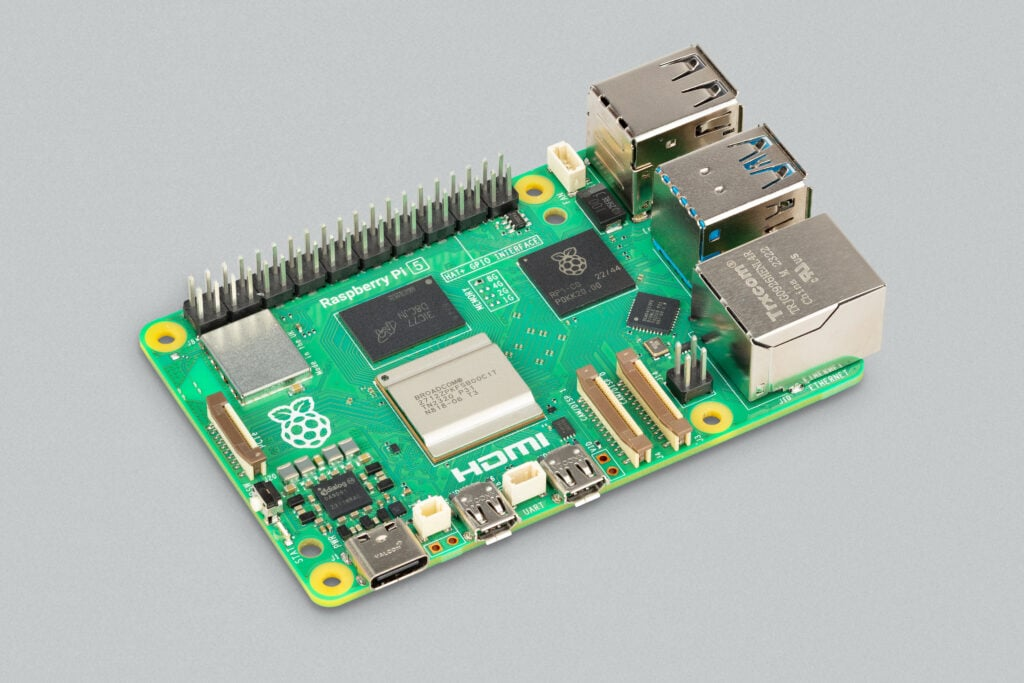
\includegraphics[width=0.4\textwidth]{figures/raspberrypi5.jpg}
    \caption{\textit{RaspberryPI5} \cite{introRaspberrypi5}}
    \label{fig:Raspberrypi5}
\end{figure}

Considerou-se, portanto, que seria uma mais-valia desenvolver um \acrshort{laboratório remoto} com as seguintes características:
\begin{itemize}
    \item \gls{python} como linguagem principal;
    \item \gls{RaspberryPI} como servidor \textit{Flask};
    \item \textit{Interface} com o utilizador desenvolvido em ~\acrfull{html}.
\end{itemize}

Estava dado o último passo na escolha do \textit{hardware} e do \textit{software} que viriam a compor o \acrshort{lare}.

\section{Solução proposta}
\label{sec:solucaoproposta}
Os objectivos principais foram apresentados na Secção \ref{sec:Objectivos} e as características gerais do projecto descritas na Secção \ref{sec:contextualização}. Pretende-se que o \acrshort{lare} seja um \acrshort{laboratório remoto} capaz de controlar e comandar um conjunto de experiências electrónicas, assim como efectuar medições de várias grandezas eléctricas. Para que a solução proposta seja completa e definitiva, é necessário definir os instrumentos de medida e os circuitos que compõem as experiências.

No contexto desta dissertação, o instrumento de medida adoptado foi o \acrfull{virtualbench}, modelo VB-8012 que pode ser controlado de duas formas: através do \textit{software} fornecido pela \acrshort{ni} ou através do \textit{pyVirtualBench}\footnote{Apesar de não ser abordado no contexto desta dissertação, existe também a possibilidade de aceder ao \acrshort{virtualbench} através do \acrshort{labview}.} \cite{AutomatingVB}. O \textit{pyVirtualBench} é um \gls{wrapper}\footnote{Este \gls{wrapper} é um \textit{software} de terceiros, suportado e mantido pela comunidade e não é diretamente suportado pela \acrshort{ni}.} que permite controlar o \acrshort{virtualbench} através de uma aplicação \gls{python} \cite{pyvirtualbench}. No entanto, este \gls{wrapper} não é compatível com \textit{Linux}.

Perante este facto, decidiu-se integrar um \acrshort{pc} no \acrshort{lare} - pormenores da instalação do \textit{driver} no \textit{site} da \acrshort{ni} \cite{AutomatingVB} - sendo que todo o peso computacional passaria para o \acrshort{pc} e o \gls{RaspberryPI} controlaria os relés. Esta decisão justifica-se pela possibilidade de, no futuro, o \textit{pyVirtualBench} vir a ser compatível com sistemas \textit{Linux}.

A outra forma de controlar o \acrshort{virtualbench} é usando a aplicação disponibilizada pela \acrshort{ni}  e compatível com \textit{Windows}. Esta aplicação faz uma apresentação integrada dos cinco instrumentos apresentados no \acrshort{virtualbench}, como pode ser visto na Figura \ref{fig:leituraohm}. A aplicação também inclui funcionalidades de fluxo de trabalho, como a importação e exportação de configurações de instrumentos e a captura de dados. Importa salientar que o \acrshort{virtualbench} não pode ser controlado simultaneamente por ambas as \textit{interfaces}.

\begin{figure}[hbtp]
    \centering
    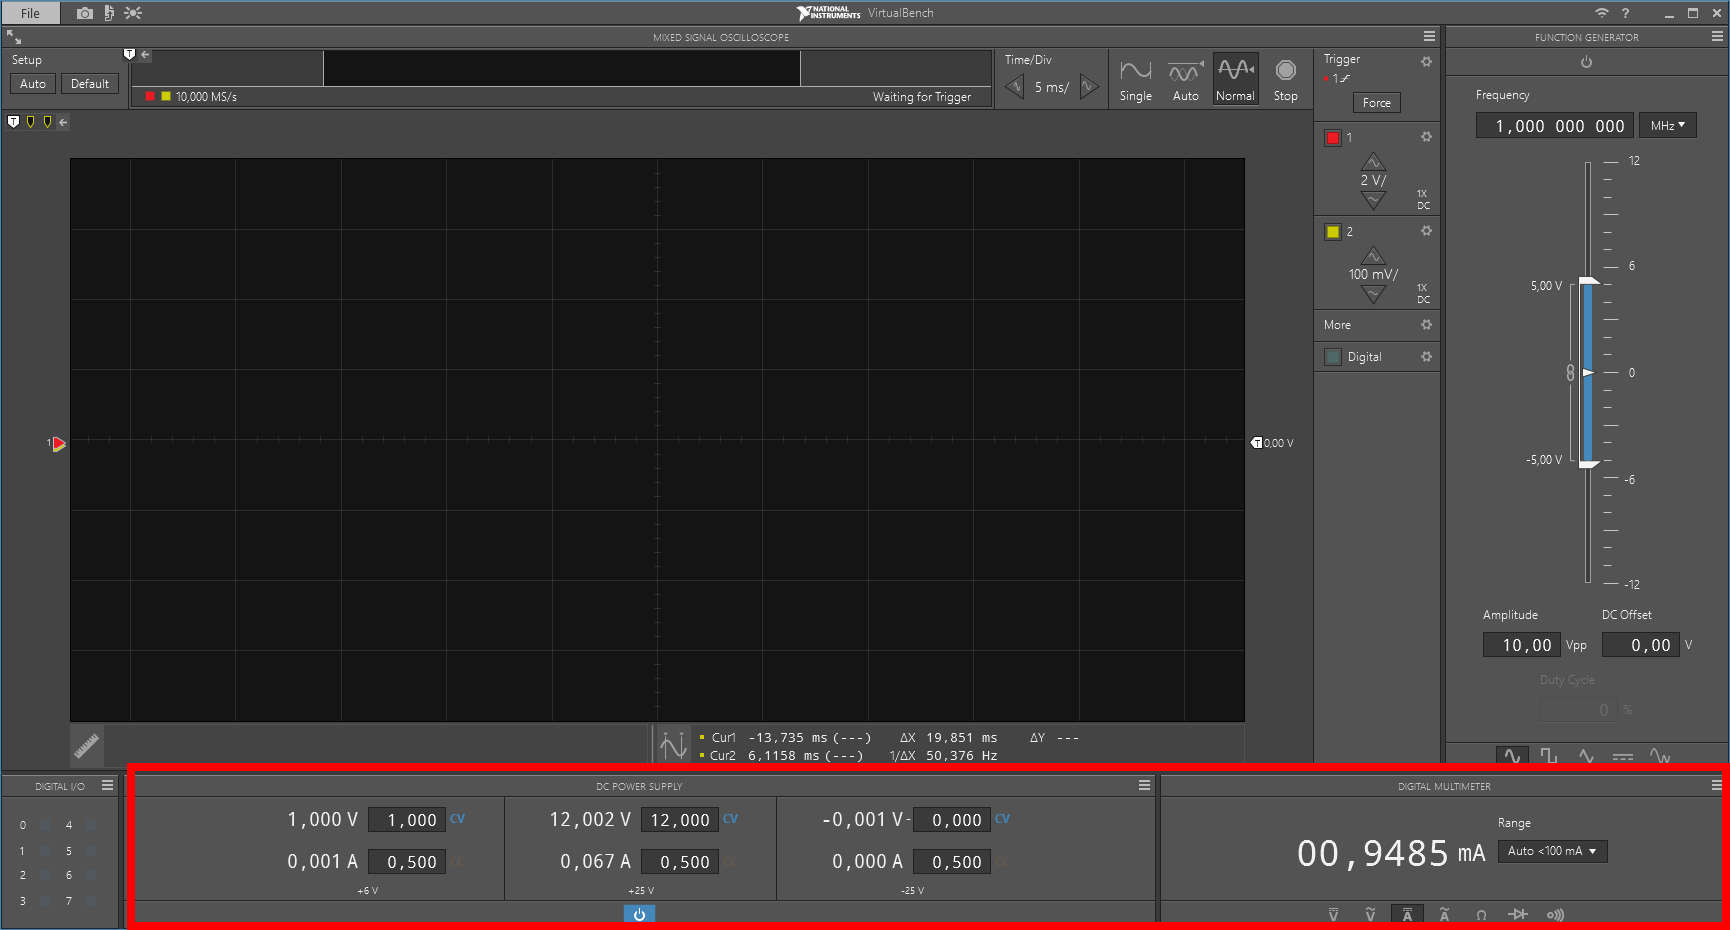
\includegraphics[width=0.7\textwidth]{figures/VB8012-OHM_Exemplo.png}
    \caption{Exemplo do \acrshort{virtualbench} usado como multímetro digital}
    \label{fig:leituraohm}
\end{figure}

As características do \acrshort{laboratório remoto} são as seguintes:
\begin{itemize}
    \item \gls{python} como linguagem principal;
    \item \acrshort{pc} como servidor \textit{Flask};
    \item \gls{RaspberryPI} como controlador dos relés;
    \item \textit{Interface} com o utilizador desenvolvido em \acrshort{html}.
\end{itemize}

Definidas - de uma forma geral - as soluções de \textit{hardware} e \textit{software}, agora com a integração de um \acrshort{pc} - passou-se ao estudo da arquitectura do \acrshort{lare}.

\section{Arquitectura}
\label{sec:arquitectura}
Como já se viu na Secção \ref{sec:contextualização}, a arquitectura do \acrshort{lare} proposta baseia-se numa estrutura cliente-servidor, suportada ao nível do \textit{hardware} pelo \acrshort{virtualbench}, pelo \gls{RaspberryPI} e um \acrshort{pc} como servidor. Uma representação geral do que será o \acrshort{lare} pode ser vista na Figura \ref{fig:representaçãogerallare}.

\begin{figure}[hbtp]
    \centering
    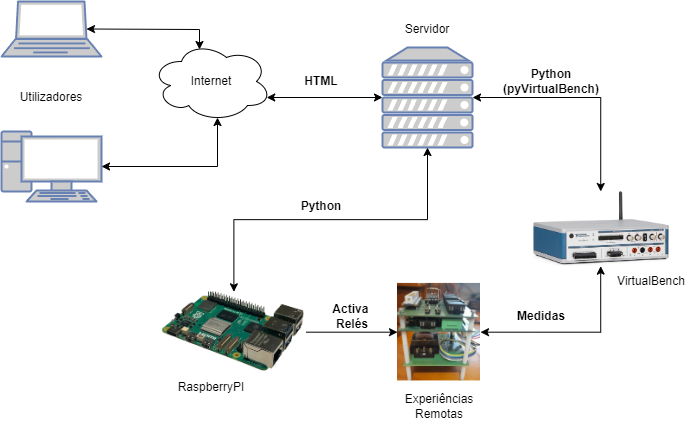
\includegraphics[width=0.7\textwidth]{figures/arquitectura_ver2.drawio.png}
    \caption{Arquitectura \acrshort{lare}}
    \label{fig:representaçãogerallare}
\end{figure}

Antes de mais, importa clarificar as formas de comunicação entre os diversos dispositivos que compõem o \acrshort{lare}. Tanto o servidor, como o \gls{RaspberryPI} e o \acrshort{virtualbench} têm disponíveis interfaces de rede sem fios e com fios, assim como \textit{interfaces} \acrshort{usb}. A comunicação entre os diversos dispositivos é feita da seguinte forma:
\begin{itemize}
    \item \textbf{Servidor - \gls{RaspberryPI}}: comunicação via rede sem fios. Para maior flexibilidade e simplicidade de programação, a comunicação entre o servidor e o \gls{RaspberryPI} é feita através da rede sem fios, utilizando \textit{sockets} que, através da sua API, facilitam a comunicação entre processos em rede, independentemente da infra-estrutura utilizada — seja por ligação com fios, sem fios ou através de redes locais, permitindo, assim, o envio e recepção de mensagens entre dispositivos ligados em rede \cite{Sockets}. O fluxograma de uma chamada ao \textit{sockets} está representado na Figura \ref{fig:fluxogramasockets};
    \item \textbf{Servidor - \acrshort{virtualbench}}: comunicação via rede sem fios ou \acrshort{usb}. Entre estes dois dispositivos é, basicamente, indiferente a forma como é feita a comunicação. Isto porque esta parte é gerida pelos \textit{drivers} da aplicação instalada no \textit{Windows}. Independentemente de se utilizar o \textit{pyVirtualBench} ou a aplicação;
    \item \textbf{Controlo de relés e medidas}: O controlo dos relés é feito através da ligação directa do \gls{RaspberryPI} ao \textit{driver} dos relés. Por sua vez, as leituras e medições das grandezas eléctricas são efectuadas pelo \acrshort{virtualbench}, ligado directamente aos pontos específicos do circuito.
\end{itemize}

\begin{figure}[hbtp]
    \centering
    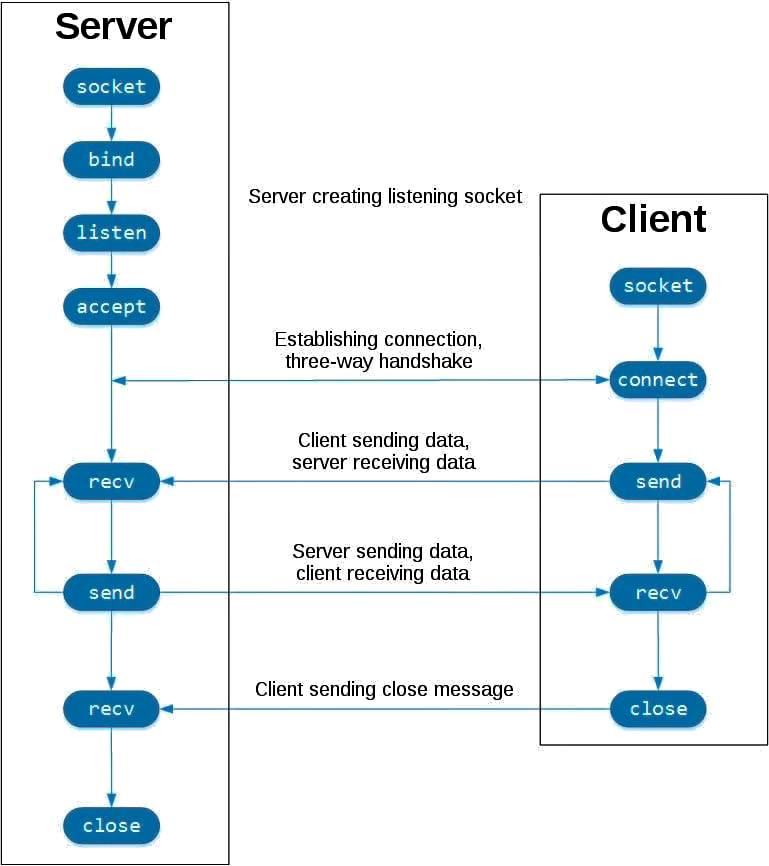
\includegraphics[width=0.5\textwidth]{figures/socketsdiagrama.png}
    \caption{Fluxograma de uma chamada ao \textit{socket} \cite{Sockets}}
    \label{fig:fluxogramasockets}
\end{figure}

Ao nível do \textit{software}, o servidor será implementado no \acrshort{pc} com base no \textit{Flask}, como já foi referido na Secção \ref{sec:contextualização} e \ref{sec:solucaoproposta}, e será descrito com mais pormenor na Secção \ref{sec:arquitecturasoftware}. A comunicação entre o servidor e o \acrshort{virtualbench}, entre o servidor e o \gls{RaspberryPI} e o controlo dos relés é feita em \textit{Python}. A \textit{interface} com o utilizador é feita em \acrshort{html}.

A Figura {\ref{fig:arquitecturalore}} apresenta com mais pormenor a solução implementada no \acrshort{lare}. De uma forma geral, podemos ver como é realizada a comunicação e a troca de informação entre os diferentes dispositivos de \textit{hardware}.

\begin{figure}[hbtp]
    \centering
    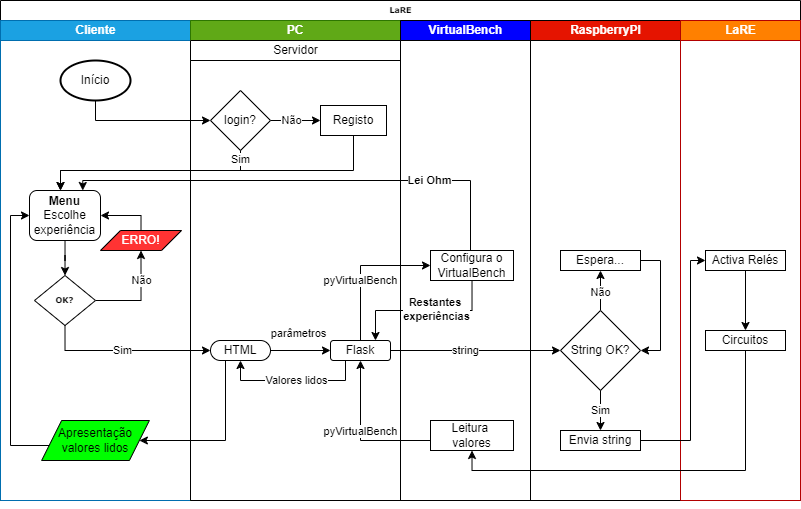
\includegraphics[width=0.7\textwidth]{figures/Diagrama_SOFTWARE.drawio.png}
    \caption{Arquitectura \acrshort{lare} - \textbf{NOTE: Fig tem de ser revista}}
    \label{fig:arquitecturalore}
\end{figure}

\section{Circuitos experimentais}
\label{sec:circuitos}
A escolha dos circuitos teve como base os que estão disponíveis no \acrshort{visir} do \acrshort{isep} e reduzindo os objectivos do \acrshort{lare} à sua forma mais básica, pode afirmar-se que se pretende ``provar um conceito''. Escolhendo experiências com circuitos integrados ou transístores, poderia tornar a implementação desnecessariamente mais complexa e, por conseguinte, com menos experiências. Portanto, o objectivo passará por criar um \acrshort{laboratório remoto} com experiências típicas para a introdução à electrónica e que permitam uma aprendizagem gradual em contexto de sala de aula. E, assim, ``provar o conceito''.

Sendo assim, os circuitos que compõem o \acrshort{lare} e satisfazem os critérios definidos em cima são:
\begin{itemize}
    \item Lei de Ohm;
    \item Rectificador de meia onda;
    \item Rectificador de onda completa;
    \item Filtro RC passa-baixo;
    \item Filtro RC passa-alto.
\end{itemize}

Doravante, considera-se que cada experiência é composta por dois circuitos distintos, com excepção da experiência dedicada à Lei de \textit{Ohm}. Por exemplo, a experiência sobre rectificação inclui os circuitos de meia onda e de onda completa; já a experiência dos filtros abrange os circuitos passa-baixo e passa-alto.

\subsection{Lei de \textit{Ohm}}
Na forma da Equação \ref{eq:leideohm}, a Lei de \textit{Ohm} estabelece que a resistência eléctrica ($R$) de um condutor é determinada pelo quociente entre a tensão elétrica ($U$) aplicada aos seus terminais e a corrente eléctrica ($I$) que o atravessa.  

\begin{equation} \label{eq:leideohm}
	R=\dfrac{U}{I}
\end{equation}

Isto significa que a Equação \ref{eq:leideohm} define uma relação linear entre a tensão e a corrente para uma determinada resistência de valor fixo, o que implica que o gráfico obtido, representado na Figura \ref{fig:graphohm}, é uma linha recta que passa pela origem. O declive dessa recta representa o valor da resistência elétrica ($R$).

\begin{figure}[hbtp]
	\centering
	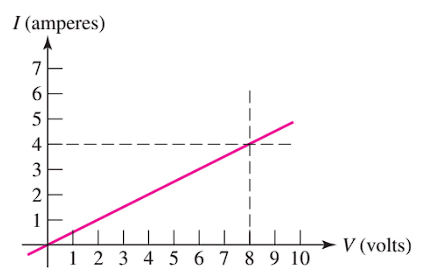
\includegraphics[width=0.3\textwidth]{figures/grafico_Ohm.png}
	\caption{Gráfico da Lei de \textit{Ohm}}
	\label{fig:graphohm}
\end{figure}

Da forma como foi implementado, há duas possibilidades de realizar este estudo, exemplificado nas Figuras \ref{fig:Opção_1} e \ref{fig:Opção_2}. O tutor ou professor, poderá optar por apresentar o conceito de duas formas distintas, em ambos os casos são efectuadas cinco medições, construido o respectivo gráfico e calculado o valor do declive da recta analiticamente. A diferença está na forma como se confrontam os resultados práticos. No entanto, no contexto desta dissertação foi  implementado o caso descrito na Figura \ref{fig:Opção_1}\footnote{Como trabalho futuro, o menu poderia ser desenvolvido para o utilizador, aluno ou professor escolher a opção pretendida.}. 

\begin{figure}[hbtp]
	\centering%
		\centering
		\subfloat[\centering Opção 1\label{fig:Opção_1}]{{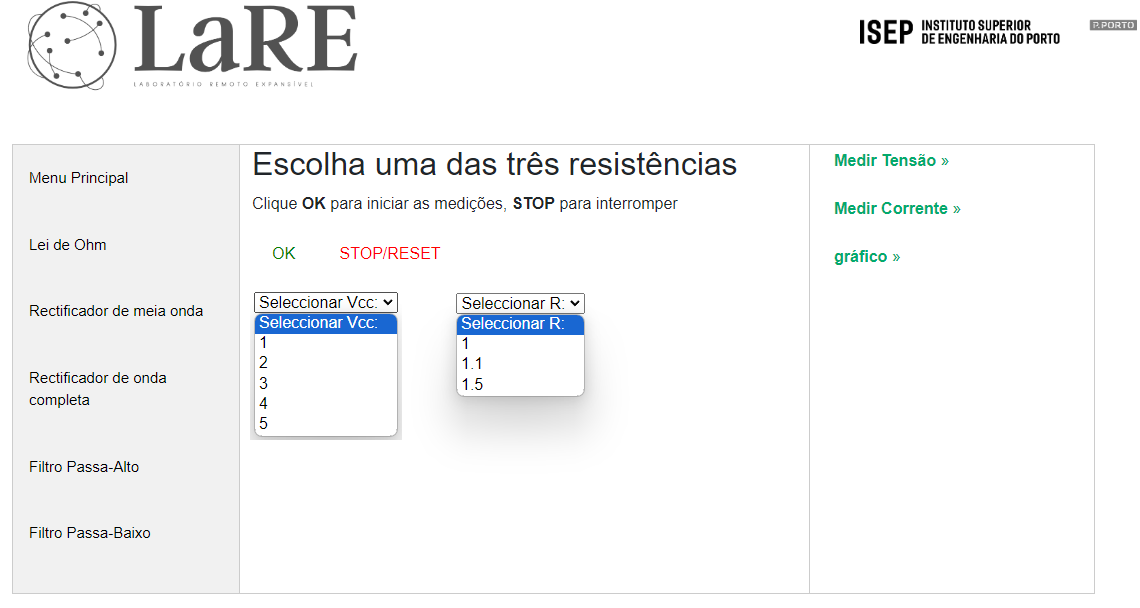
\includegraphics[width=6.3cm]{figures/ohm_escolha.png} }}%
		\qquad
		\subfloat[\centering Opção 2\label{fig:Opção_2}]{{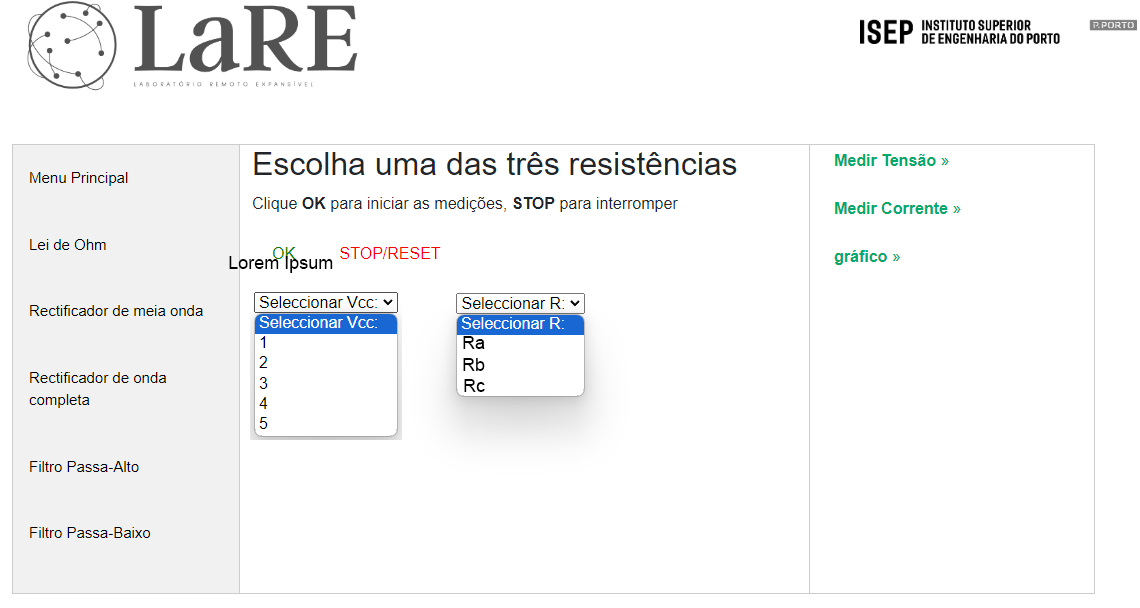
\includegraphics[width=6.3cm]{figures/ohm_escolha_abc.png} }}%
		\caption{Experiência Lei de \textit{Ohm}}%
		\label{fig:experienciaOHM}%
	\end{figure}

No caso em que a resistência é dada, o declive pode ser calculado e confrontado com as soluções, sendo que no caso em que é desconhecida, o declive da recta é calculado e a partir deste do resultado infere-se o valor da resistência. 

\subsection{Rectificadores}
\label{sec:circuitosrectificadores}
Nas experiências dos rectificadores pretende-se estudar e avaliar a diferença entre os dois tipos de rectificação, consoante as quatro combinações possíveis dos pares resistência/condensador e a influência que têm na variação da tensão de \textit{ripple}. No caso da rectificação de meia onda, é ainda possível variar a frequência entre os \SI{50}{\hertz} e \SI{2000}{\hertz} - \textbf{NOTA: Estes limites podem ter que ser ajustados} mas no caso da rectificação de onda completa, a frequência é fixa ao valor da rede eléctrica - \SI{50}{\hertz}.

A Figura~\ref{fig:blocosrectificacao} apresenta o diagrama de blocos simplificado do processo de rectificação, que pode ser usado, por exemplo, para o projecto duma fonte de alimentação em contexto de sala de aula. Este é composto por quatro blocos principais:

\begin{itemize}
    \item Bloco 1 - Transformador: reduz a tensão proveniente da rede eléctrica para valores mais baixos e adequada ao nível de tensão alternada que se deseja;
    \item Bloco 2 - Rectificação: realiza a conversão da tensão alternada \acrshort{ca} em tensão contínua unidirecional, ainda com ondulação;
    \item Bloco 3 - Filtragem: responsável pela suavização da forma de onda, reduzindo a componente alternada (\textit{ripple});
    \item Bloco 4 - Estabilização:  regula e estabiliza a tensão de saída, garantindo um valor contínuo e constante.
\end{itemize}

\begin{figure}[hbtp]
	\centering
	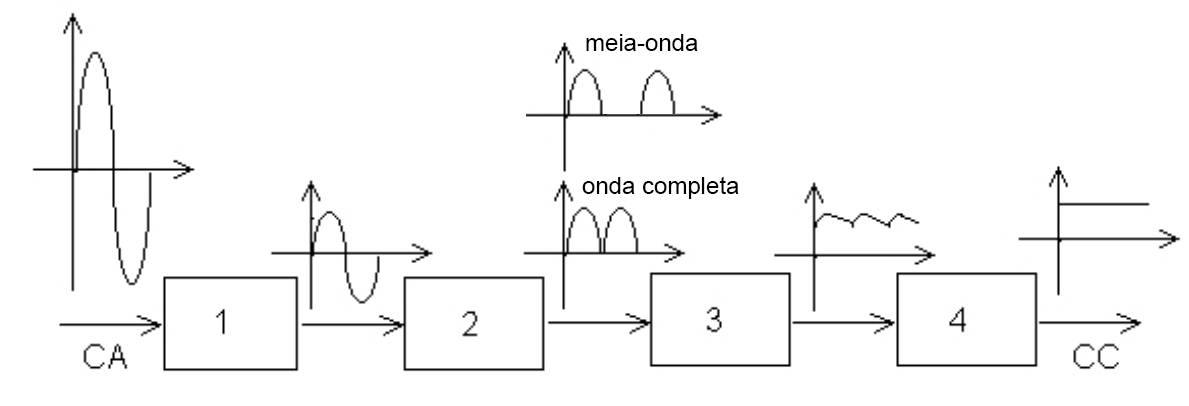
\includegraphics[width=0.7\textwidth]{figures/diagramablocosrectificacao.png}
	\caption{Diagrama de blocos da rectificação \textins{meia onda e onda completa}}
	\label{fig:blocosrectificacao}
\end{figure}

A tensão de \textit{ripple} é uma componente variável no tempo que surge à saída da filtragem, Bloco 3, como representado na Figura \ref{fig:blocosrectificacao}. Esta componente deve ser minimizada para estabilizar a tensão de saída em corrente contínua, Bloco 4, representado na mesma figura \cite{sedrasmith}. A Figura \ref{fig:sedraripple} representa a forma de onda à saída do Bloco 3 - Filtragem - quando se utiliza a rectificação de meia onda.
\begin{figure}[hbtp]
	\centering
	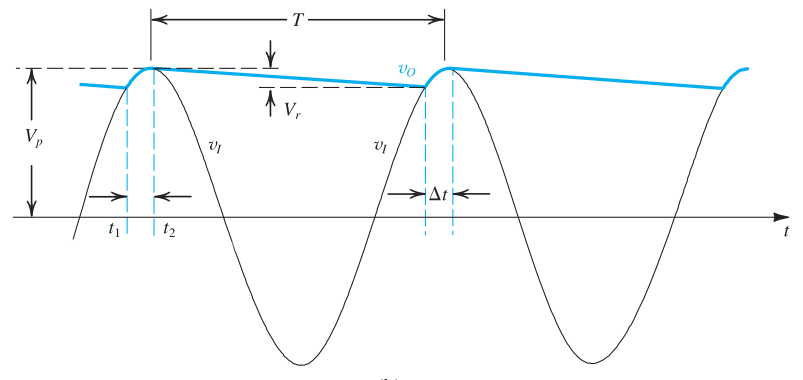
\includegraphics[width=0.7\textwidth]{figures/sedra_ripple.png}
	\caption{Forma de onda à saída do Bloco 3 - Filtragem [meia onda] \cite{sedrasmith}}
	\label{fig:sedraripple}
\end{figure}

A tensão de \textit{ripple} pode ser calculada através da Equação \ref{eq:vripplecompleta}:

\begin{equation} \label{eq:vripplecompleta}
	U_{r} = U_{P}(1-e^{-\frac{T}{RC}})
\end{equation}

Observa-se, a partir da Equação \ref{eq:vripplecompleta}, que quando a constante de tempo $RC >> T$, o cálculo da tensão de \textit{ripple} pode ser reduzido à Equação \ref{eq:vripple}.

\begin{equation} \label{eq:vripple}
	U_{r} = \frac{U_{P}}{fRC}
\end{equation}

Sendo que, neste caso, a tensão de \textit{ripple} é baixa e $v_{o}$, ou seja, a tensão à saída do filtro é practicamente constante e dada pela Equação \ref{eq:tensaosaida}:

\begin{equation} \label{eq:tensaosaida}
	u_{o} = U_{P} - \dfrac{1}{2}U_{r}	
\end{equation}

No entanto, pode tornar-se este circuito mais eficiente se se usar a rectificação de onda completa e como pode ser visto na Figura \ref{fig:sedraripplecompleta}, a frequência do \textit{ripple} é o dobro da frequência da onda de entrada.

\begin{figure}[hbtp]
	\centering
	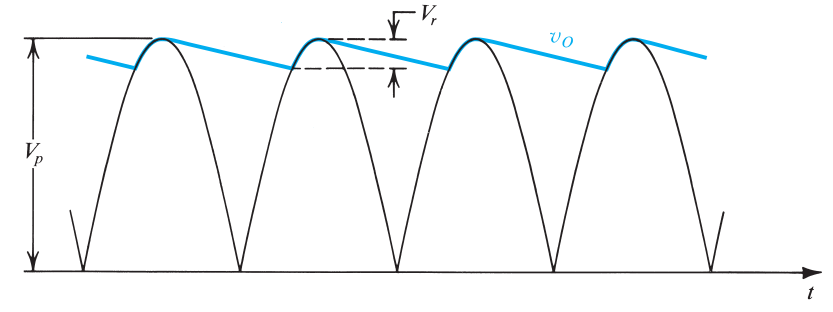
\includegraphics[width=0.7\textwidth]{figures/sedra_ripple_OC.png}
	\caption{Forma de onda à saída do Bloco 3 - Filtragem [onda completa] \cite{sedrasmith}}
	\label{fig:sedraripplecompleta}
\end{figure}

Sendo assim, o valor da tensão de \textit{ripple}, neste caso, será dado pela Equação \ref{eq:vrippleOC}:

\begin{equation} \label{eq:vrippleOC}
	U_{r} = \frac{U_{P}}{2fRC}
\end{equation}

São estas formas de onda, representadas pelas Figuras \ref{fig:sedraripple} e \ref{fig:sedraripplecompleta}, que se pretendem estudar e avaliar, assim como os valores dados pelas Equações \ref{eq:vripple} e \ref{eq:vrippleOC}. (A Equação \ref{eq:vripplecompleta} deve ser usada quando os valores dos condensadores e resistências são pequenos ou frequência é baixa, isto é, quando o \textit{ripple} não é desprezável.)

\subsection{Filtros}
Representados na Figura \ref{fig:filtrosesqgeral} estão os filtros simplificados, leccionados em contexto de sala de aula no ensino secundário.

\begin{figure}[hbtp]
	\centering%
		\centering
		\subfloat[\centering Filtro passa-baixo\label{fig:filtro_pb}]{{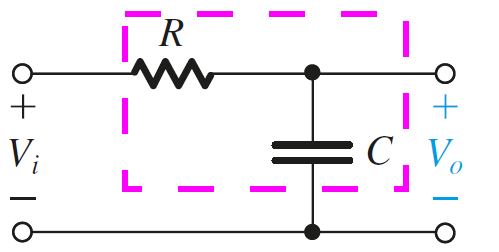
\includegraphics[width=6cm]{figures/Sedra_FPB_GIMP.png} }}%
		\qquad
		\subfloat[\centering Filtro passa-alto\label{fig:filtro_pa}]{{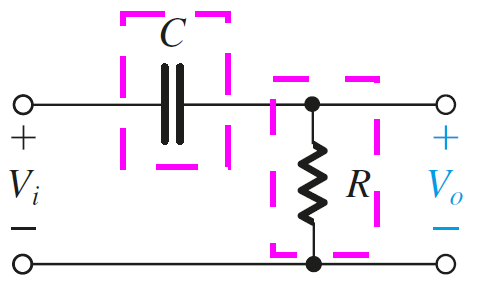
\includegraphics[width=6cm]{figures/Sedra_FPA_GIMP.png} }}%
		\caption{Esquemas dos filtros \cite{sedrasmith}}%
		\label{fig:filtrosesqgeral}%
\end{figure}

A possibilidade de variar a frequência do sinal de entrada permite que estas experiências sejam utilizadas para estudar a resposta em frequência dos filtros, analisar o Diagrama de \textit{Bode}, determinar a frequência de corte dada pela Equação \ref{eq:frequenciacorte} e ainda relacionar, por exemplo, o valor da tensão de entrada com a tensão de saída. 

\begin{equation} \label{eq:frequenciacorte}
	f_{c} = \frac{1}{2\pi RC}
\end{equation}

As Figuras \ref{fig:Bode_pb} e \ref{fig:Bode_pa} apresentam os Diagramas de \textit{Bode} \textins{ideais}, que servem de referência para o estudo desta experiência. 

\begin{figure}[hbtp]
	\centering%
		\centering
		\subfloat[\centering Filtro passa-baixo\label{fig:Bode_pb}]{{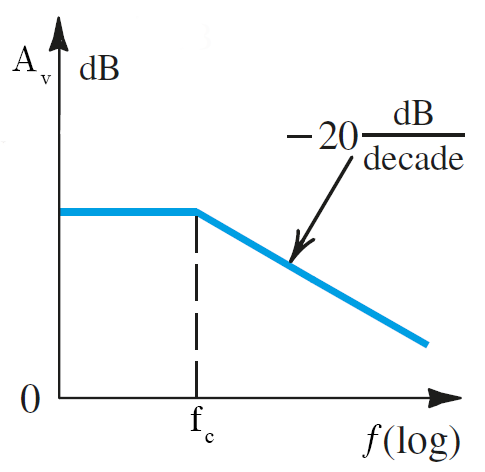
\includegraphics[width=6cm]{figures/Sedra_BodeFPB.png} }}%
		\qquad
		\subfloat[\centering Filtro passa-alto\label{fig:Bode_pa}]{{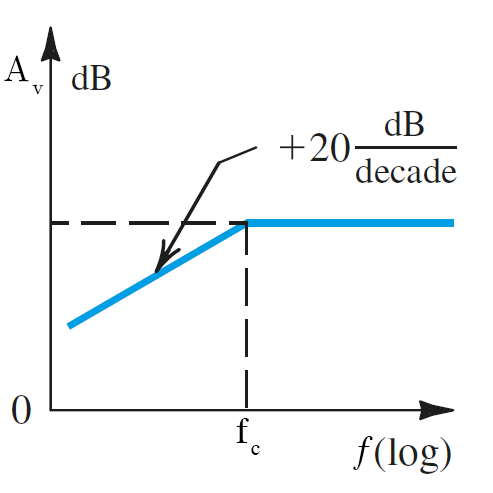
\includegraphics[width=6cm]{figures/Sedra_BodeFPA.png} }}%
		\caption{Diagramas de \textit{Bode} \textins{ideal} \cite{sedrasmith}}%
		\label{fig:Bodeesqgeral}%
\end{figure}

	Para além da análise em frequência, um outro aspeto complementar a considerar é a relação entre as ondas de entrada e saída, em função da frequência. Nos filtros, o intervalo de frequências permitido é igual ao já referido para os rectificadores: entre \SI{50}{\hertz} a \SI{80000}{\hertz}. 
	
	A frequência de corte de um filtro é definida como o ponto onde o ganho do filtro sofre uma atenuação de \SI{3}{\decibel} em relação ao seu valor máximo. 	Para um filtro passa-baixo (passa-alto) ideal, o ganho em baixas (altas) frequências é unitário. Quando o sinal atinge a frequência de corte, a relação entre a tensão de saída e a tensão de entrada reduz-se para:  
	
	\begin{equation} \label{eq:relacaoGanho}
		\frac{U_{out}}{U_{in}} = \frac{1}{\sqrt{2}} \approx 0.707
	\end{equation}
	
	\ldots ou na escala logarítmica:  
\begin{equation} \label{eq:relacaoGanhodB}
	\frac{U_{out}}{U_{in}} = 20 \log_{10} (0.707) \approx -\SI{3}{\decibel}	
\end{equation}
	
Assim, a frequência de corte de um filtro corresponde ao ponto em que a amplitude do sinal de saída é aproximadamente $70.7\%$ da amplitude do sinal de entrada, o que corresponde a -\SI{3}{\decibel}. 

\section{Hardware}
\label{sec:hardware}
\subsection{VirtualBench}
Este dispositivo desenvolvido pela \acrshort{ni} integra vários instrumentos e ferramentas de teste, tais como um osciloscópio digital com análise de protocolo, um gerador de formas de onda, um multímetro digital, uma fonte de alimentação \acrfull{cc} programável e E/S digitais num único dispositivo que se liga a um \acrshort{pc}, via \acrshort{usb} ou rede sem fios, como se pode ver na Figura \ref{fig:paineltraseiro}. As principais características deste modelo estão descritas na Figura \ref{fig:paineldianteiro} \cite{datasheetVirtualBench}. A forma como pode ser controlado e configurado já foi abordada na Secção \ref{sec:solucaoproposta}.

\begin{figure}[hbtp]
    \centering
    \centering
    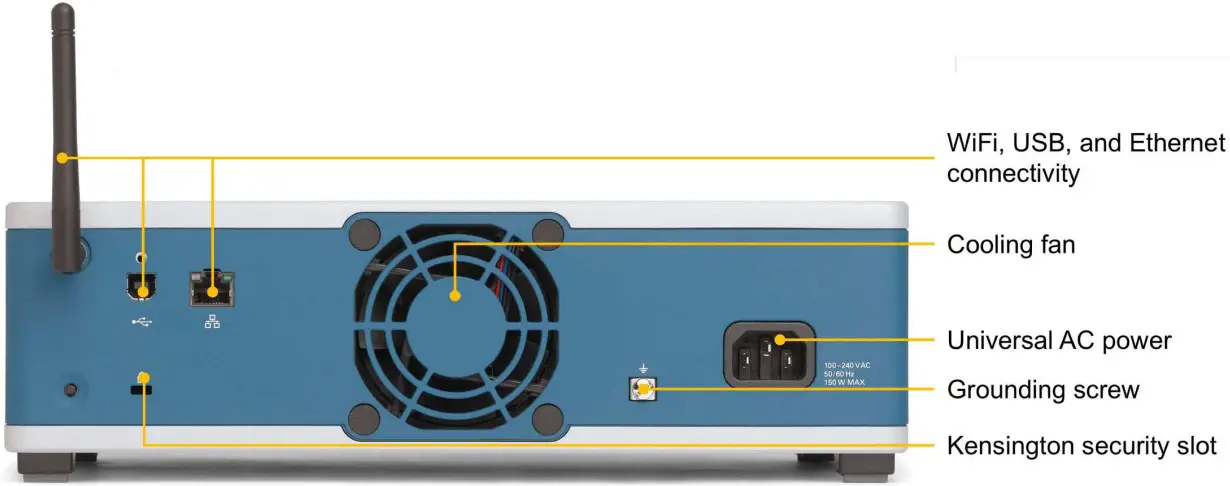
\includegraphics[width=0.5\textwidth]{figures/virtualbench_back-panel.jpg}
    \caption{Painel traseiro \textit{VirtualBench} VB-8012  \cite{datasheetVirtualBench}.}
    \label{fig:paineltraseiro}
\end{figure}

\begin{figure}[hbtp]
    \centering
    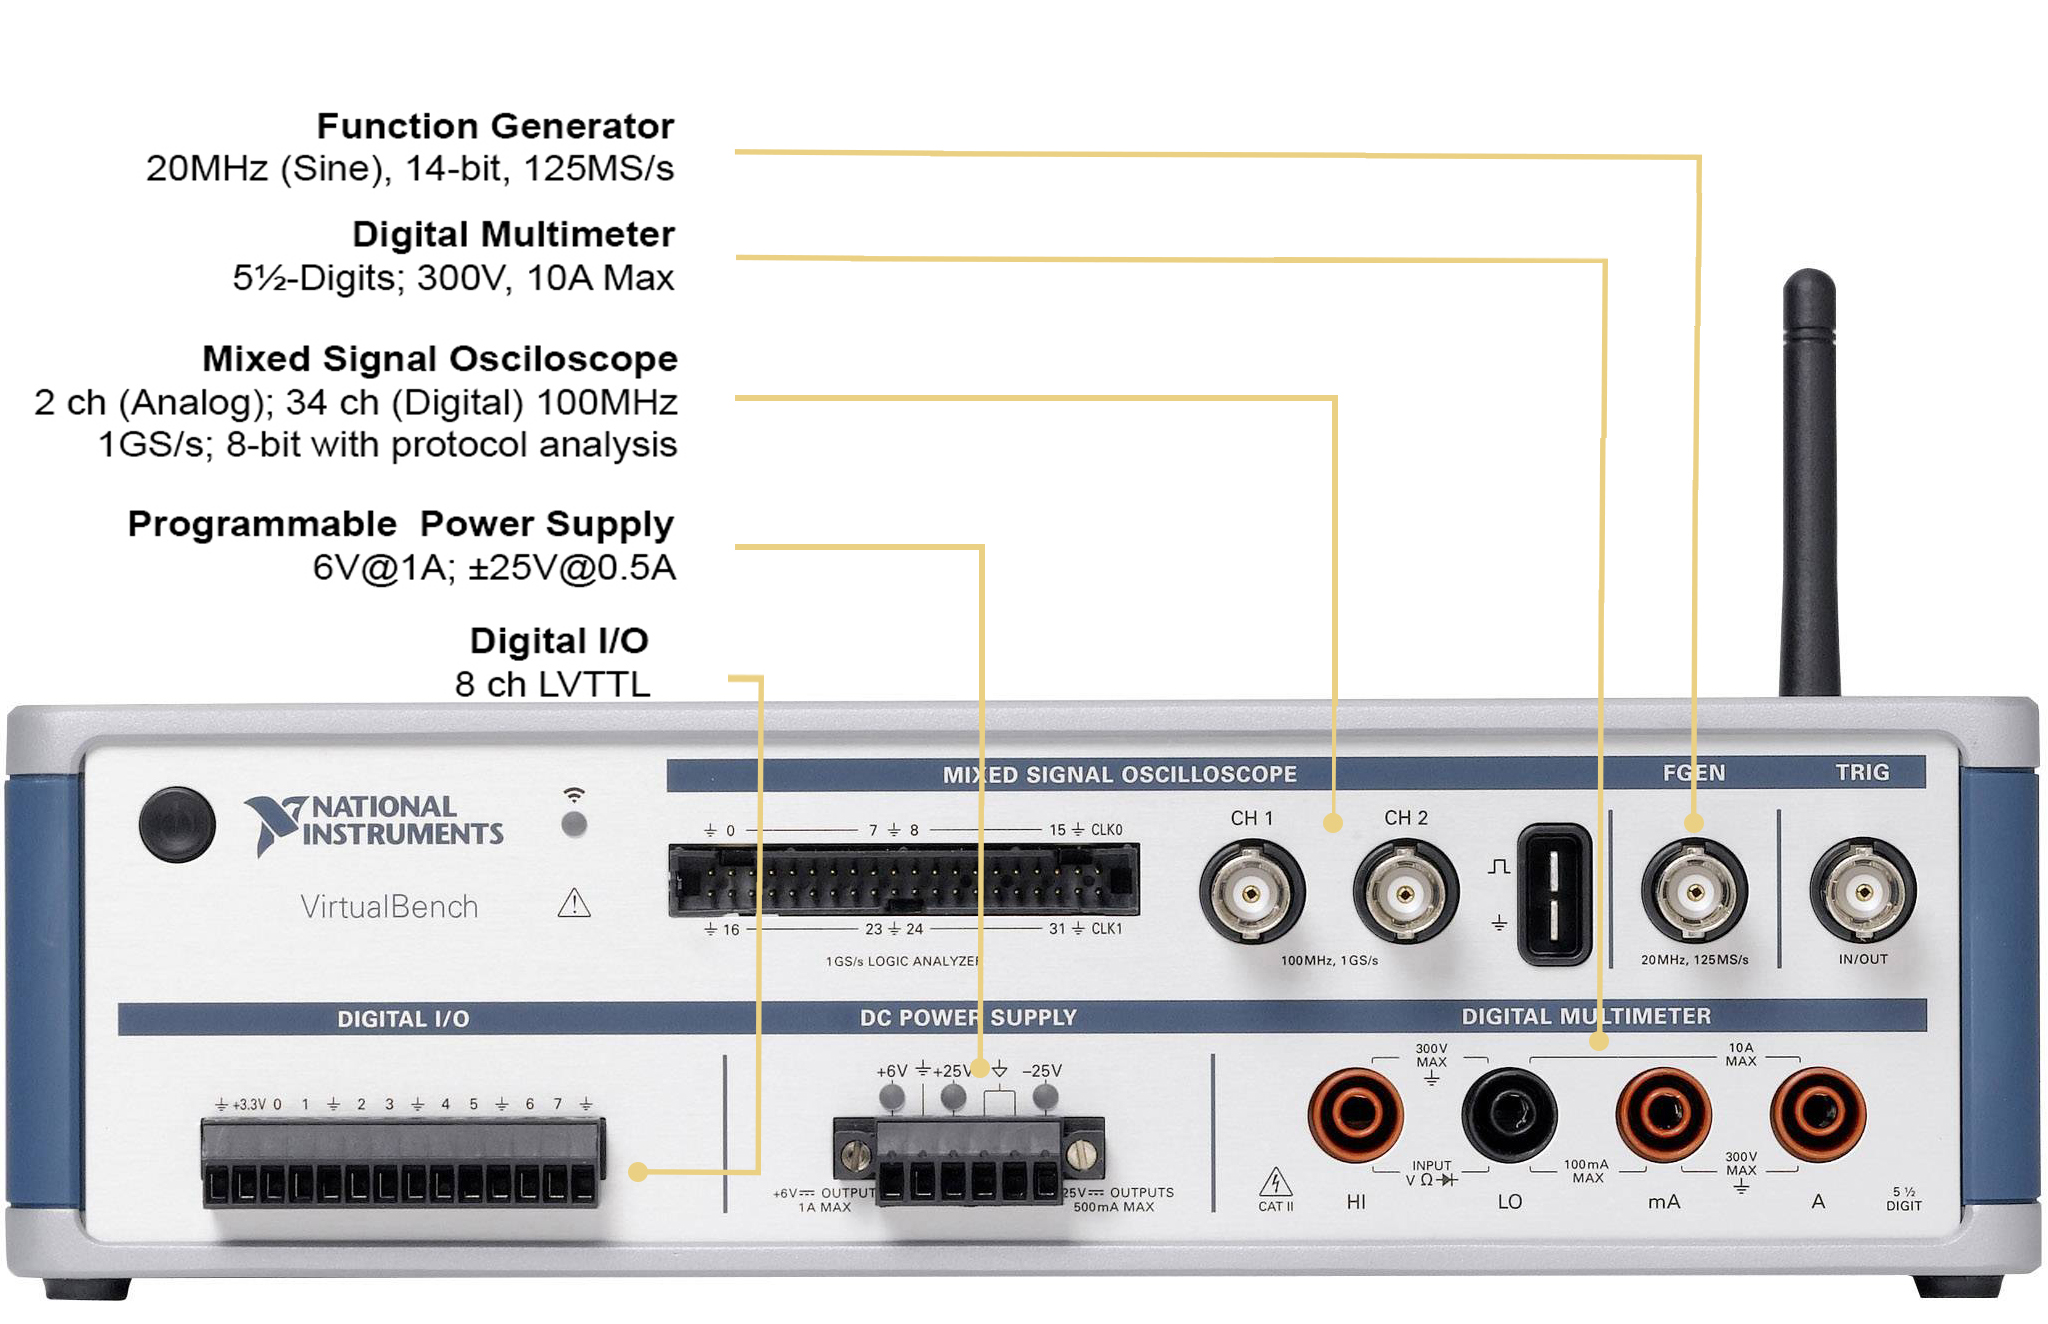
\includegraphics[width=0.5\textwidth]{figures/virtualbench_front-panel.jpg}
    \caption{Painel frontal \textit{VirtualBench} VB-8012  \cite{datasheetVirtualBench}.}
    \label{fig:paineldianteiro}
\end{figure}

\subsection{Matriz LaRE}
\label{sec:matriz}
Definidas as soluções de \textit{hardware} e \textit{software}, bem como as experiências a implementar, iniciou-se o projecto da matriz. Tal como anteriormente, e tendo o \acrshort{visir} como referência, decidiu-se desenvolver uma matriz cujas placas respeitem as dimensões definidas pelo consórcio \gls{pc/104} \cite{PC104}, o qual estabelece um padrão caracterizado pelo seu formato compacto e modular.

Os esquemas finais das experiências encontram-se no Anexo \ref{AppendixA}, onde se pode verificar que o número de relés necessários varia entre 8 — no caso da Lei de \textit{Ohm} — e 13 — nos casos dos rectificadores e dos filtros. Sendo assim, com o objectivo de facilitar a implementação, os testes, a detecção de erros e, mais tarde, a manutenção, optou-se por dividir o \acrshort{lare} em três placas. O desenho dos esquemas e dos \acrfull{pcb} foram elaborados com recurso ao \gls{kicad}. A Figura \ref{fig:matrizlare} apresenta uma visão geral da matriz do \acrshort{lare}. 

\begin{figure}[hbtp]
	\centering
	\includegraphics[width=0.4\textwidth]{figures/lare_3placas.png}
	\caption{Matriz do \acrshort{lare}}
	\label{fig:matrizlare}
\end{figure}

\subsubsection{Lei de \textit{Ohm}}
A placa desenvolvida para esta experiência está representada na Figura \ref{fig:placaleideohm}:

\begin{figure}[hbtp]
	\centering
	\includegraphics[width=0.5\textwidth]{figures/lare_ohm_BLOCOS.png}
	\caption{\textins{Placa} Lei de \textit{Ohm}}
	\label{fig:placaleideohm}
\end{figure}

\begin{enumerate}
	\item Ligação ao \gls{RaspberryPI} através de um conector \acrfull{idc} de 40 pinos (1);
	\item Relés (2);
	\item Ligações aos aparelhos de medida (3);
	\item \textit{Drivers} de relés e registo de deslocamento (4);
	\item Resistências em estudo (5);
	\item Ligação à placa seguinte através de conectores ``Arduino stackable'' (6).
\end{enumerate}

\subsubsection{Rectificadores/Filtros}
A Figura \ref{fig:placarectificadores} apresenta a placa da experiência referente aos rectificadores/filtros:

\begin{figure}[hbtp]
	\centering
	\includegraphics[width=0.5\textwidth]{figures/lare_rectificador_filtros_BLOCOS.png}
	\caption{\textins{Placa} rectificadores e filtros}
	\label{fig:placarectificadores}
\end{figure}
 
\begin{enumerate}
	\item Rectificação;
		\begin{enumerate}
			\item \label{diodos}Díodo rectificador - meia onda ($1_{a}$) e Ponte rectificadora - onda completa ($1_{b}$);	
		\end{enumerate}
    \item Relés (2);
    \item Resistências - \textins{componentes comuns a ambas as experiência}(3);
  	\item \textit{Drivers} de relés e registo de deslocamento (4);
	\item Condensadores \textins{componentes comuns a ambas as experiências}(5);
	\item Ligação à placa seguinte através de conectores ``Arduino stackable'' (6);
	\item Resistência e condensador exclusivo dos filtros (7).
\end{enumerate}

\subsubsection{Fontes de alimentação}
A placa referente às fontes de alimentação está representada na Figura \ref{fig:placartransformador}. Esta placa é constituída por um transformador e uma fonte de \SI{5}{\volt}. O esquema completo está disponível no Anexo \ref{AppendixA}.

\begin{figure}[hbtp]
	\centering
	\includegraphics[width=0.3\textwidth]{figures//lore_fonte.jpg}
	\caption{\textins{Placa} fontes de alimentação}
	\label{fig:placartransformador}
\end{figure}

\begin{comment}
\begin{figure}[hbtp]
    \centering
    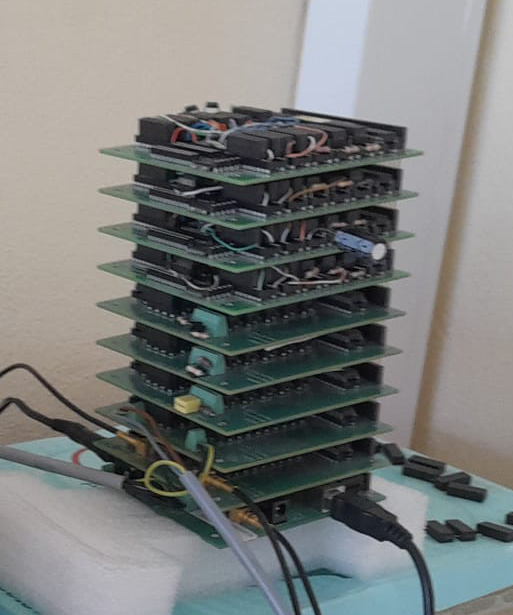
\includegraphics[width=0.3\textwidth]{figures/promenorvisirISEP.png}
    \caption{Placas PC/104 do \acrshort{visir} - \acrshort{isep} - \textbf{Foto com melhor qualidade}}
    \label{fig:visir104}
\end{figure}
\end{comment}

\subsection{Raspberry Pi}
\label{sec:RaspberryPI}
Como já foi referido na Secção \ref{sec:contextualização}, a ideia inicial passava por utilizar o \gls{RaspberryPI} como servidor e como controlador dos relés, no fundo desempenhando as funções de \acrshort{rlms}. Este dispositivo insere-se numa gama de pequenos computadores de placa única \gls{sbc}, acessíveis e versáteis, como o \textit{Banana Pi}, \textit{BeagleBone Black}, \textit{Orange Pi} ou \textit{Odroid}, amplamente utilizados em ensino, prototipagem e aplicações de \acrshort{iot}. 

Em contexto de laboratório estavam disponíveis os modelos PI2 e PI3, algo desactualizados. O PI3 já se mostrou lento nos primeiros testes e, por isso, optou-se pela última versão do \gls{RaspberryPI}, que à data da escrita deste documento é a 5. Esta versão traz várias melhorias e novos recursos, sendo que as principais diferenças de \textit{hardware} para a versão 4B estão representadas na Tabela \ref{Table:diferencasPI4PI5}. No entanto, estas melhorias acarretam um maior consumo de energia e, por isso, é recomendado o uso de arrefecimento activo \cite{Raspberrytech}. Na Figura \ref{fig:pi5dissipador} está representado o \gls{RaspberryPI} usado no \acrshort{lare}.

\begin{figure}[hbtp]
    \centering
    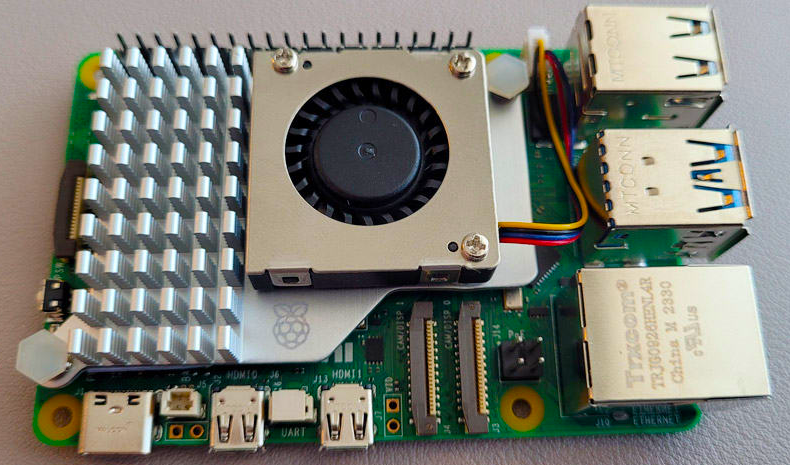
\includegraphics[width=0.5\textwidth]{figures/pi5_dissipador.png}
    \caption{\textit{Raspberry PI5} com dissipador activo utilizado no \acrshort{lare}}
    \label{fig:pi5dissipador}
\end{figure}

\begin{table}[htb]
    \centering
    \caption{Raspberry PI4 \textit{vs Raspberry PI5 - principais diferenças} \cite{Raspberrypi5}}
    \label{Table:diferencasPI4PI5}
    \begin{tabular}{ll}
        \toprule
        Raspberry PI4                                            & Raspberry PI5                                             \\
        \midrule
        \SI{1.8}{\giga\hertz}                                    & \SI{2.4}{\giga\hertz}                                     \\
        \midrule
        VideoCore VI @ \SI{500}{\mega\hertz}, Vulkan 1.0         & VideoCore VII @ \SI{800}{\mega\hertz}, Vulkan 1.2         \\
        \midrule
        LPDDR4-3200 SDRAM até \SI{8}{\giga\byte}                 & LPDDR4X-4267 SDRAM \SI{4}{\giga\byte}/\SI{8}{\giga\hertz} \\
        \midrule
        \SI{5}{\volt}/\SI{3}{\ampere} via USB-C (\SI{15}{\watt}) & \SI{5}{\volt}/\SI{5}{\ampere} via USB-C (\SI{27}{\watt})  \\
        \bottomrule
    \end{tabular}
\end{table}

Comum às versões anteriores, o \gls{RaspberryPI} possui um conector de 40 pinos denominados \acrfull{gpio}s, como se pode ver na Figura~\ref{fig:gpio}. Os \acrshort{gpio}s são pinos versáteis e configuráveis e permitem que a placa interaja com uma variedade de componentes eletrónicos e outros dispositivos, como por exemplo, relés, sensores, motores, etc.. Os \acrshort{gpio}s são pinos digitais, isto é, o \gls{RaspberryPI} não possui um \acrfull{adc} interno para ler sinais analógicos. No entanto, pode usar-se um \acrshort{adc} externo, como por exemplo, o MCP3008 ou o módulo ADS1115. Quer isto dizer que só trabalham com duas tensões: \SI{3.3}{\volt} ou \SI{0}{\volt}, correspondendo aos valores lógicos ``1'' ou ``0'', respectivamente. Dependendo da configuração dos \acrshort{gpio}s - entrada ou saída - estes podem ler ou fornecer as tensões correspondentes aos níveis lógicos desejados. 

\begin{figure}[hbtp]
    \centering
    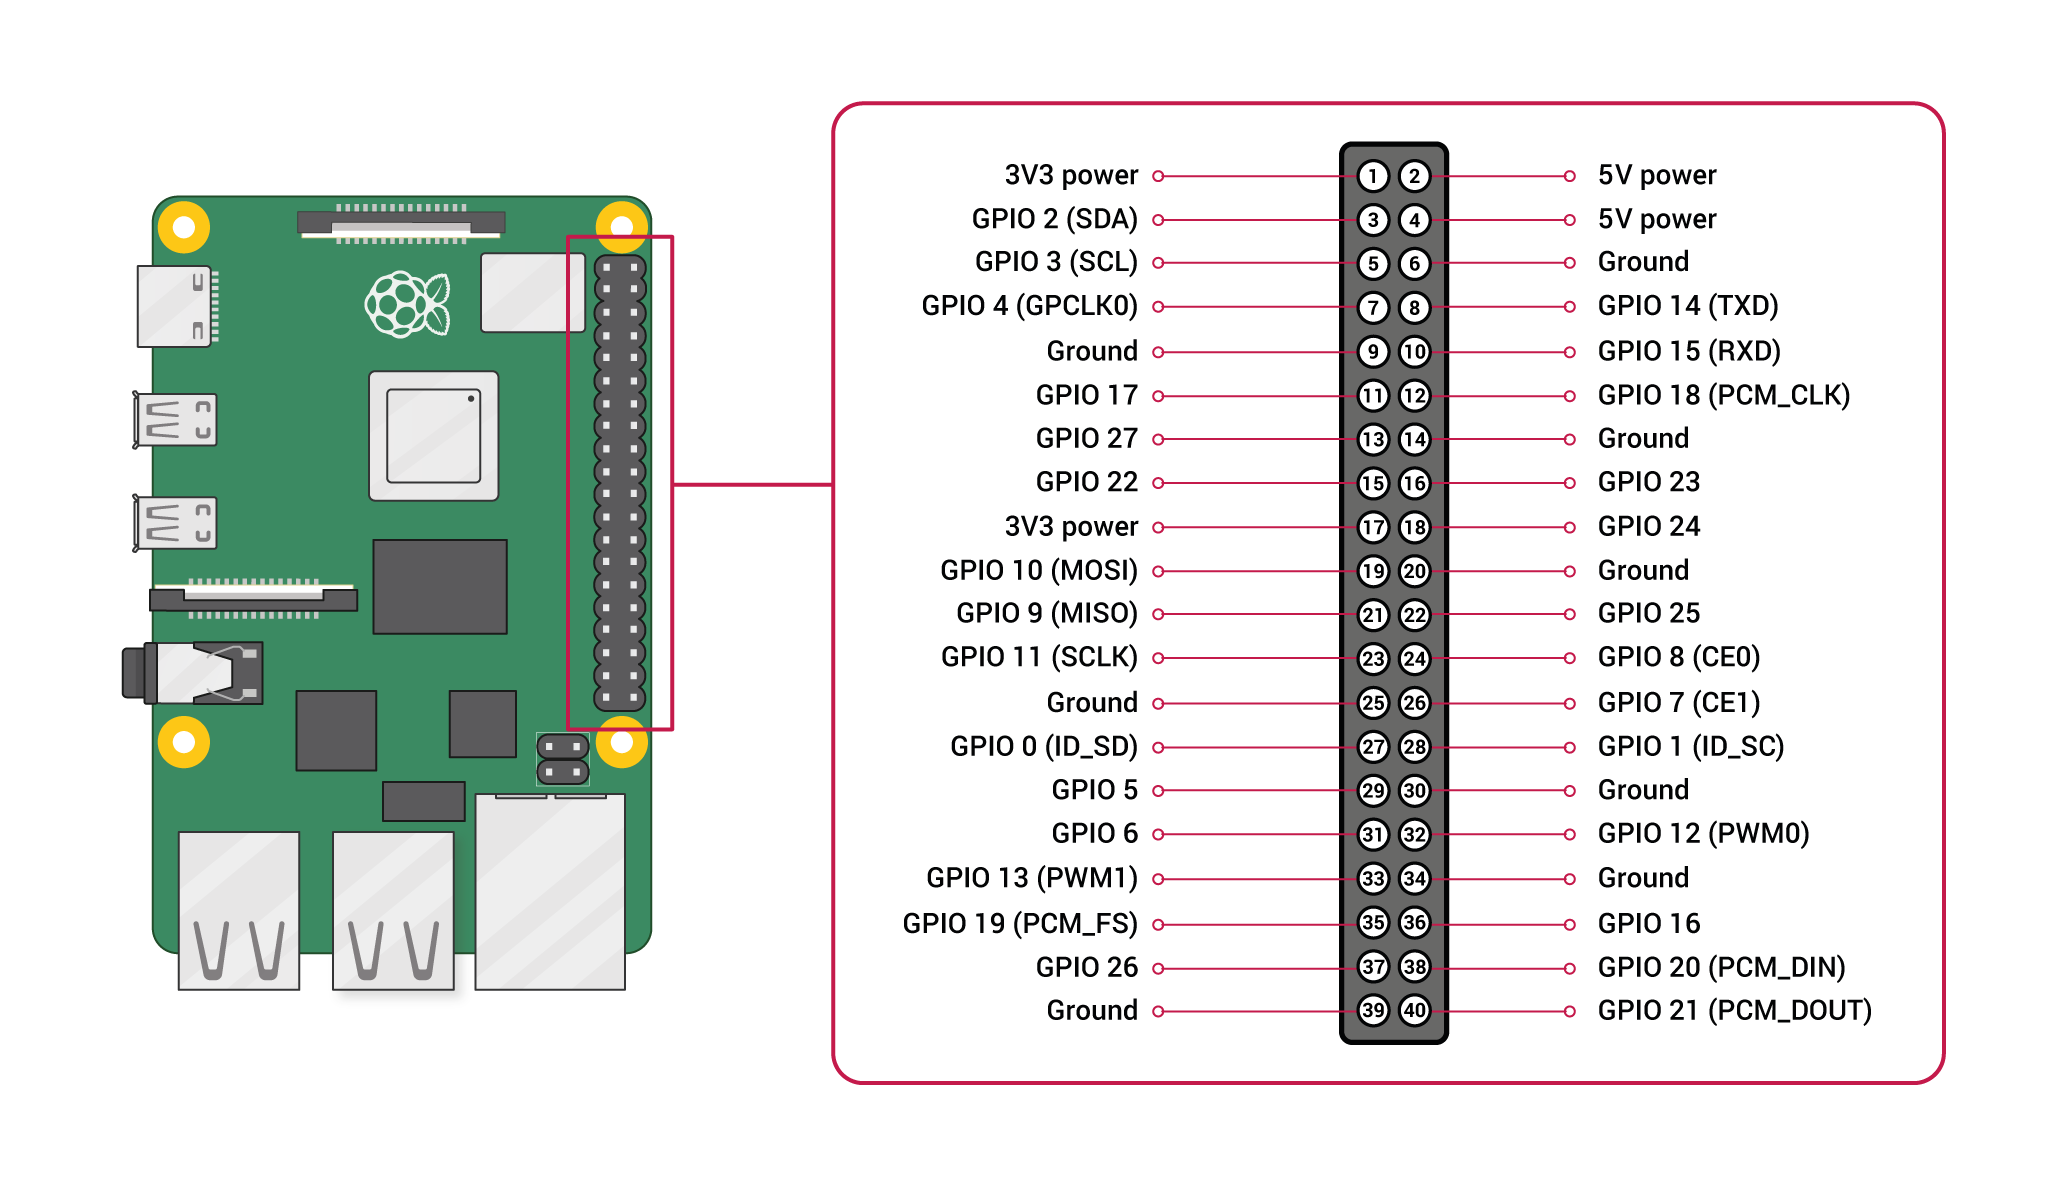
\includegraphics[width=0.5\textwidth]{figures/GPIO-Pinout-Diagram-2.png}
    \caption{\acrshort{gpio}s \textit{RaspberryPI} \cite{Raspberrytech}}
    \label{fig:gpio}
\end{figure}

A corrente no \gls{RaspberryPI} pode ser configurada para valores entre \SI{2}{\milli\ampere} e \SI{16}{\milli\ampere} (em intervalos de \SI{2}{\milli\ampere}) por cada \acrshort{gpio}. No entanto, quando vários \acrshort{gpio}s são utilizados em simultâneo, o valor total combinado da corrente não deve exceder os \SI{50}{\milli\ampere}. Se for fornecida uma tensão superior a \SI{3.3}{\volt} aos \acrshort{gpio}s, o \gls{RaspberryPI} corre o risco de se danificar irremediavelmente. \cite{Raspberrytech}. Na Figura \ref{fig:gpiocores} está representada uma forma alternativa de visualizar os \acrshort{gpio}s, mais intuitiva e que permite perceber melhor a função dos pinos. Representados a cor amarela estão os \acrshort{gpio}s que podem ser configurados como entrada ou saída; a vermelho, laranja e preto as alimentações de \SI{5}{\volt}, \SI{3.3}{\volt} e \textit{ground}, respectivamentee. Por fim, os \acrshort{gpio}s representados pela cor branca, \acrshort{gpio}0  e \acrshort{gpio}1, correspondentes aos pinos físicos 27 e 28, respectivamente, estão reservados para utilização avançada, nomeadamente, a comunicação \acrshort{i2c} com a \gls{eeprom} de identificação presente em \gls{hat}s compatíveis. Esta \gls{eeprom} permite a configuração automática do sistema aquando do arranque. 

\begin{figure}[hbtp]
    \centering
    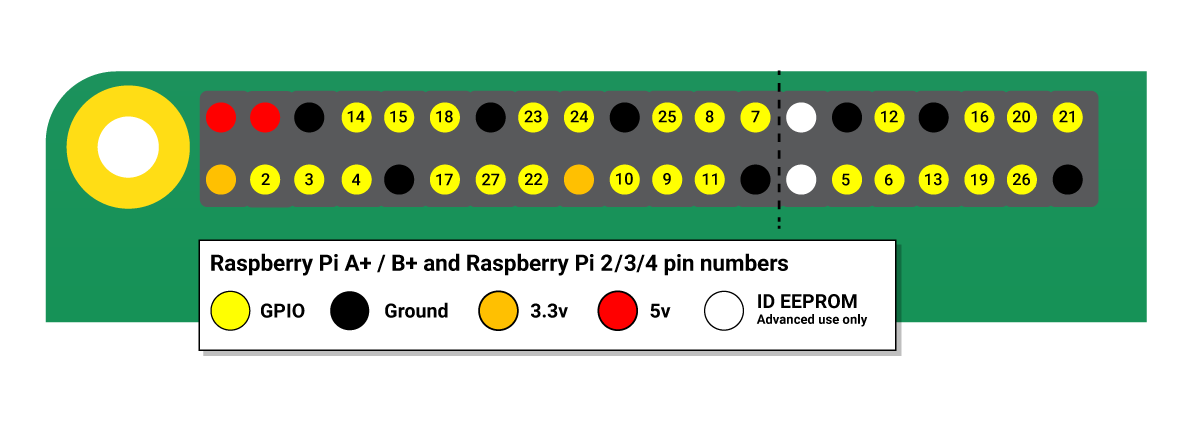
\includegraphics[width=0.5\textwidth]{figures/GPIO.png}
    \caption{Representação alternativa dos \acrshort{gpio}s \cite{Raspberrytech}}
    \label{fig:gpiocores}
\end{figure}

\subsection{Relés}
\label{sec:reles}
Como já foi referido na Capítulo \ref{Capitulo2}, os circuitos que compõem o \acrshort{visir} são controlados através de relés. Estes dispositivos funcionam como interruptores electromecânicos simples que utilizam um sinal elétrico para controlar um eletroíman.
Os relés electromecânicos são constituídos por uma bobine e um contacto, que pode ser normalmente aberto ou fechado. A corrente eléctrica ao passar pela bobine gera um campo magnético que atrai o contacto, fechando-o ou abrindo-o, conforme o caso. A Figura \ref{fig:esquematicoreles} mostra um esquema simplificado de um relé electromecânico, onde se pode observar a inclusão do díodo de ``roda livre'', comum em muitos circuitos de comando com relés. Este díodo é utilizado para proteger o circuito de comando de picos de tensão induzidos pela bobine do relé, quando a corrente é desligada, segundo a Lei de Faraday. O díodo permite que a corrente induzida pela bobine circule em circuito fechado, evitando danos nos componentes de comando. 

\begin{figure}[hbtp]
    \centering
    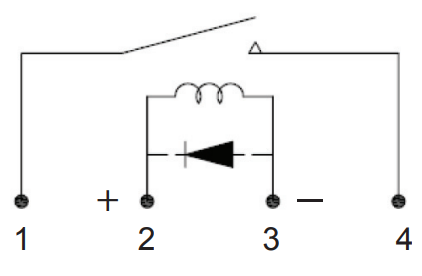
\includegraphics[width=0.3\textwidth]{figures/esquematico_rele.png}
    \caption{\textit{Esquema simplificado de um relé \cite{DryRelay}}}
    \label{fig:esquematicoreles}
\end{figure}

Os relés utilizados no \acrshort{lare} estavam disponíveis em contexto laboratorial e são em tudo idênticos aos que se encontram instalados no \acrshort{visir}  do \acrshort{isep}. Foram usados dois tipos de relés: simples (\acrfull{spst}) e duplos (\acrfull{dpst}), como ilustrado na Figura \ref {fig:reles}. Ambos os modelos são da marca \textit{Comus} - o relé \acrshort{spst}, ref. 3570-1331-123 e o relé \acrshort{dpst}, ref. 3572-1220-123. As características principais encontram-se descritas no Anexo~\ref{AppendixA} e as completas nos respectivos \textit{datasheet} \cite{DryRelay}. 

Nos códigos de referência dos relés, os dois primeiros quartetos indicam a série, enquanto os três dígitos indicam a tensão nominal da bobine e a presença, ou não, do díodo de ``roda livre''. No caso dos modelos utilizados, esta tensão é de \SI{12}{\volt} e o díodo está ligado entre os pinos 2(+) e 6(-) \cite{DryRelay}. Sempre que possível, tentou-se utilizar os relés \acrshort{spst} no comando das fontes e aparelhos de medida e os relés \acrshort{dpst} no controlo dos componentes. Serão devidamente referidos os casos em que isso não foi possível, por indisponibilidade dos componentes.

\begin{figure}[hbtp]
    \centering
    \includegraphics[width=0.5\textwidth]{figures/reles.png}
    \caption{\textit{Relés \acrshort{spst} e \acrshort{dpst}} \cite{DryRelay}}
    \label{fig:reles}
\end{figure}

Como já foi referido na Secção \ref{sec:RaspberryPI}, a tensão de funcionamento dos \acrshort{gpio}s, quer estejam configurados como entrada ou saída, é de \SI{3.3}{\volt}, sendo que a máxima corrente por cada \acrshort{gpio} é de \SI{16}{\mA}.
Com estes valores, o \gls{RaspberryPI} não tem capacidade para comandar os relés, já que funcionam a \SI{12}{\volt}. Para activar os relés, é necessário o uso de \textit{drivers}\footnote{Doravante, sempre que for referido o termo \textit{driver} no contexto de relés, subentende-se o circuito integrado \textit{ULN2003A}.} que consigam fornecer a tensão e corrente necessárias para o efeito.

\subsection{\textit{Driver} de Relés}
\label{sec:driver}
O circuito integrado ULN2003A, é um \textit{driver} muito usado para controlar relés. Além disso estava disponível em contexto laboratorial. Tipicamente, é usado em conjunto com microcontroladores ou \gls{RaspberryPI}\footnote{Importa distinguir entre \gls{sbc}s, como o \gls{RaspberryPI} e microcontroladores, como o Arduino. Enquanto os \gls{sbc}s funcionam como computadores completos capazes de executar sistemas operativos e aplicações complexas, os microcontroladores são dispositivos mais simples, ideais para tarefas de controlo directo, operando sem sistema operativo e com recursos significativamente mais limitados.} no comando de cargas indutivas, como motores, bobines e relés. Estes \textit{drivers} possuem sete pares de transístores NPN, em configuração \textit{Darlington}, que apresentam saídas de alta tensão com díodos \textit{clamp} de cátodo comum para comutação de cargas indutivas \cite{ULN2003}, como se  representa esquematicamente na Figura \ref{fig:2003blocos}.

\begin{figure}[hbtp]
    \centering
    \includegraphics[width=0.5\textwidth]{figures/2003A_Darling.png}
    \caption{Diagrama de blocos ULN2003A \cite{ULN2003}}
    \label{fig:2003blocos}
\end{figure}

A corrente de colector de saída (única) é de \SI{500}{\mA} e a corrente de entrada, para uma tensão de entrada de \SI{3.85}{\volt}, é \SI{0.93}{\mA} \cite{ULN2003}.

Pela análise dos esquemas, representados no Anexo \ref{AppendixA} e já referenciado na Secção \ref{sec:matriz}, verifica-se que os \acrshort{gpio}s disponíveis no \gls{RaspberryPI} - 26 no total - não são suficientes para comandar os relés do \acrshort{lare}. Ao todo são utilizados 21 relés, o que corresponderia a 21 saídas, faltando adicionar 10 \acrshort{gpio}s necessários para o controlo da transmissão das \textit{strings} de \textit{bits}. Sendo assim, houve a necessidade de criar uma solução que permitisse comandar os relés, já que o \gls{RaspberryPI} não possui \acrshort{gpio}s suficientes.

\subsection{Registo de deslocamento}
\label{sec:registodeslocamento}
O uso de registos de deslocamento foi a solução encontrada de forma a ultrapassar o problema da falta de \acrshort{gpio}s. O \textit{SN74HC595}\footnote{Doravante, sempre que for referido registo de deslocamento, subentende-se o circuito integrado \textit{SN74HC595}.} é um circuito integrado comum e bastante utilizado que contém um registo de deslocamento de 8 \textit{bits} com saídas \textit{3-State}, do tipo \acrfull{sipo}, que alimenta um registo de armazenamento do tipo D, também de 8 \textit{bits} e com saídas paralelas \textit{3-State}. O sinal de relógio para o registo de deslocamento e armazenamento é independente. A potência consumida é muito baixa, assim como a corrente de entrada \cite{SN74HC595}.

Descrição dos pinos de controlo:
\begin{itemize}
    \item \acrfull{ser}: é utilizado para enviar os \textit{bits} para o registo de deslocamento, um \textit{bit} de cada vez;

    \item \acrfull{srclk}: é o relógio do registo de deslocamento e é ativado no flanco ascendente, por cada impulso dado um \textit{bit} é enviado para o registo de deslocamento;

    \item \acrfull{rclk}: é o relógio do do registo de armazenamento e é activo no flanco ascendente. Quando activo, o conteúdo do registo de deslocamento é transferido para o registo de armazenamento, que eventualmente aparece na saída;

    \item \acrfull{srclr}: permite fazer o \textit{clear} ou \textit{reset} ao registo de deslocamento. Isto equivale a colocar todos os \textit{bits} a zero. Este pino é activo baixo.

    \item \acrfull{oe}: pino activo baixo que controla o estado da saída do registo: Se a zero as saídas estão activas, se a um as saídas estão desactivadas
\end{itemize}

Como referido na Secção~\ref{sec:matriz}, a experiência da Lei de \textit{Ohm} requer 8 relés, enquanto as experiências de rectificadores e filtros necessitam de 13. Cada relé é acionado por um \textit{bit} de um registo de deslocamento, sendo que cada registo permite o controlo de até 8 relés. Assim, é necessário um registo para a experiência da Lei de \textit{Ohm} e dois registos para as experiências de rectificação e filtragem.
Deste modo, é enviada uma \textit{string} de 8 ou 13 \textit{bits}, conforme a experiência a controlar - os \textit{bits} são enviados um-a-um, armazenados no registo e depois enviados para a saída. Dado que o número de \textit{bits} varia entre experiências e estas se encontram distribuídas por duas placas distintas (conforme descrito na Secção~\ref{sec:matriz}), optou-se por utilizar pinos diferentes do \gls{RaspberryPI} para o envio das \textit{strings}. No Anexo \ref{AppendixA}, Figura 11 e Figura 12, estão definidos os pinos usados na configuração e envio das \textit{strings}. A Figura~\ref{fig:SN74HC595blocos} apresenta o diagrama de blocos do registo de deslocamento, enquanto a Tabela~\ref{Table:funcSN74HC595} descreve os seus modos de funcionamento. Como se pode observar, o controlo do envio de uma \textit{string} de dados requer 5 pinos \acrshort{gpio} configurados como saídas. Deste modo, para comandar os relés das experiências distribuídas pelas duas placas, são necessários 10 pinos \acrshort{gpio} no total.

\begin{figure}[hbtp]
    \centering
    \includegraphics[width=0.7\textwidth]{figures/SR_blocos.png}
    \caption{Diagrama \textins{em corte} de blocos SN74HC595 \cite{SN74HC595}}
    \label{fig:SN74HC595blocos}
\end{figure}

Importa notar que seria tecnicamente possível reduzir este número para apenas 6 pinos, utilizando os mesmos sinais de controlo para ambos os registos de deslocamento e activando-os seletivamente através da linha \textit{OE - Output Enable} de cada registo. No entanto, dado que a implementação e os testes dos circuitos foram realizados de forma faseada, optou-se por manter conjuntos de pinos independentes para cada registo de deslocamento, facilitando a deteção e resolução de eventuais erros. As implicações ao nível do \textit{software} de programação são mínimas e ao nível do \textit{hardware} estão dentro dos limites de número de \acrshort{gpio}s do \gls{RaspberryPI}.

\begin{table}[htb]
    \caption{Modos de funcionamento do SN74HC595 \cite{SN74HC595}}
    \label{Table:funcSN74HC595}
    \resizebox{\textwidth}{!}{%
        \begin{tabular}{cccccl}
            \toprule
            \multicolumn{5}{c}{Entradas}           & \multicolumn{1}{c}{\multirow{3}{*}{Função}}                                                                                        \\
            \cline {1-5}
            \multicolumn{5}{l}{}                   &
            \multicolumn{1}{c}{}                                                                                                                                                        \\
            \multicolumn{1}{l}{SER}                &
            \multicolumn{1}{l}{SRCLK}              &
            \multicolumn{1}{l}{$\overline{SRCLR}$} &
            \multicolumn{1}{l}{RCLK}               &
            \multicolumn{1}{l}{$\overline{OE}$}    &
            \multicolumn{1}{c}{}                                                                                                                                                        \\
            \midrule
            X                                      & X                                           & X & X          & H & Saídas $Q_A$ - $Q_H$ estão desabilitadas.                       \\
            \midrule
            X                                      & X                                           & X & X          & L & Saídas $Q_A$ - $Q_H$ estão habilitadas.                         \\
            \midrule
            X                                      & X                                           & L & X          & X & Registo de deslocamento é limpo.                                \\
            \midrule
            L                                      &
            $\uparrow$                             &
            H                                      &
            X                                      &
            X                                      &
            \begin{tabular}[c]{@{}l@{}} Primeiro passo do registo de deslocamento vai a ``0''. \\ Passo seguinte armazena os dados do estado anterior, respectivamente. \end{tabular}   \\
            \midrule
            H                                      &
            $\uparrow$                             &
            H                                      &
            X                                      &
            X                                      &
            \begin{tabular}[c]{@{}l@{}}Primeiro passo do registo de deslocamento vai a ``1''. \\ Passo seguinte armazena os dados do estado anterior, respectivamente. \end{tabular}    \\
            \midrule
            X                                      & X                                           & X & $\uparrow$ & X & Os dados do registo de deslocamento são armazenados no registo. \\
            \bottomrule
        \end{tabular}%
    }
\end{table}

\section{Software}
\label{sec:arquitecturasoftware} 
O \textit{software} do \acrshort{lare} foi dividido em duas grandes partes: \textit{Back-end} e \textit{Front-end}.

Por \textit{Back-end} entende-se toda a programação e os processos que correm em segundo plano w que sustentam o funcionamento do \acrshort{lare}, incluindo o servidor, as \acrshort{api}s ou base de dados \cite{FrontbackEnd}. Existem diversas linguagens de programação, \textit{frameworks} e ferramentas para gerir esta parte do sistema. Na implementação do \acrshort{lare}, foi utilizada a linguagem \textit{Python}, em conjunto com a \textit{Framework} \textit{Flask} .

O \textit{Front-end}, por sua vez, gere a \textit{interface} do \textit{site}, ou seja, a camada com que o utilizador interage directamente. As linguagens utilizadas na sua implementação foram o \acrshort{html}, \acrfull{css} e \textit{JavaScript}. Enquanto o \acrshort{html} constitui a estrutura base da página, o \acrshort{css} define o estilo visual dos elementos o \textit{JavaScript} permite a criação de comportamentos dinâmicos e interactivos \cite{FrontbackEnd}.

De forma resumida, o desenvolvimento de \textit{Front-end} corresponde ao lado do cliente (aspecto da página \textit{Web}), enquanto o \textit{Back-end} diz respeito ao lado do servidor (funcionamento da página \textit{Web}).

\subsection{\textit{Back-End}}
\label{sec:back-end}
\subsubsection{\textit{Python}}
O \textit{Python} é uma linguagem poderosa e fácil de aprender. Possui estruturas de dados de alto nível eficientes e uma abordagem simples, mas eficaz à programação orientada para objectos \cite{ThePython}. Apresenta, também, uma série de vantagens que se enquadram nos objectivos do desenvolvimento e implementação do \acrshort{lare} \cite{pythonvantagens}:
\begin{itemize}
    \item Curva suave de aprendizagem;
    \item Quantidade e variedade das bibliotecas;
    \item Portabilidade;
    \item Flexibilidade;
    \item Robustez;
    \item Suporte da comunidade.
\end{itemize}

Como desvantagens há a referir que, comparado com outras linguagens, o \textit{Python} é mais lento em termos de execução, já que é um tipo de linguagem de alto-nível, pelo que não é adaptado para aplicações móveis e consome mais recursos \cite{pythonvantagens} \cite{5MainDispython}. Ainda assim, segundo a \textit{IEEE Spectrum} \cite{ieeespectrum}, a linguagem \textit{Python} foi considerada a mais popular em 2023.

\subsubsection{\textit{Flask}}
O \textit{Flask} é uma \textit{framework} leve e flexível para \textit{Python} que segue a filosofia \textit{UNIX} de ``fazer uma coisa bem feita''. A escolha do \textit{Flask} deveu-se, essencialmente, à facilidade de integração com o \textit{Python}, sendo uma das \textit{frameworks} mais populares em \textit{Python} \cite{Flask}. É uma \textit{framework} de aplicações \acrfull{wsgi} que descreve a forma como um servidor \textit{Web} comunica com aplicações \textit{Web} e como essas aplicações podem ser encadeadas para processar um pedido \cite{wsgi}. Depende, ainda do  \textit{Jinja}, que é um motor de criação de modelos que permite escrever código semelhante à sintaxe do \textit{Python}, de forma a renderizar o documento final \cite{Jinja}.

Tal como foi referido na Secção \ref{sec:contextualização}, foram ainda analisadas várias opções, incluindo a \textit{Django}, outra \textit{framework} bastante popular. Em \cite{Djangovsflask} e \cite{FlaskvsDjango}, por exemplo, é feita uma comparação exaustiva entre as duas \textit{frameworks}, não havendo uma decisão final sobre qual a melhor, mas sim sobre qual a que melhor se adapta às necessidades de implementação e desenvolvimento dos projectos. No entanto, o \textit{Flask} foi concebido para tornar a iniciação rápida e fácil, com a capacidade de evoluir até aplicações mais complexas, sendo mais adapatado a pequenos projectos.

Tendo em conta os argumentos anteriormente apresentados e a análise dos respetivos prós e contras, considerou-se que a linguagem de programação \textit{Python}, em conjugação com o \textit{Flask} enquanto \textit{framework} para desenvolvimento de aplicações web e APIs, constitui a solução que melhor se enquadra e adapta aos objectivos definidos para o \acrshort{lare}.

\subsubsection{\textit{Jinja2}}
\label{sec:jinja2}
O \textit{Jinja2}\footnote{O nome \textit{Jinja2} refere-se à versão actual do sistema de \textit{templates} Jinja, resultante de uma reescrita significativa da sua versão original. Na documentação e na comunidade, é comum referir-se a este motor simplesmente como \textit{Jinja} \cite{Jinja}. Assim, e sem perda de generalidade, será adoptada ao longo deste trabalho a designação \textit{Jinja}.} é um sistema de \textit{templates} para aplicações \textit{Web} escrito em \textit{Python}, amplamente utilizado em conjunto com a \textit{framework} \textit{Flask}. O seu principal objetivo é permitir a separação entre a lógica da aplicação e a apresentação visual, promovendo um desenvolvimento mais organizado, modular e sustentável. Inspirado na sintaxe do próprio \textit{Python}, o \textit{Jinja} permite incorporar estruturas de controlo, como ciclos e condições, diretamente nos ficheiros \acrshort{html} através de marcação específica, facilitando a criação dinâmica de conteúdo \cite{Jinja}. Na Listagem \ref{lst:exemplojinja} pode ver-se um exemplo de código \textit{Jinja} incluído na página \textit{base.html}.

\begin{minipage}{0.9\linewidth}
    \begin{lstlisting}[language=python, caption=Exemplo \textit{Jinja} incluído na página \textit{base.html}, label=lst:exemplojinja]
	<title>Home</title>
    
        <a class="nav-item nav-link" id="home" href="/">Home</a>
    
        <a class="nav-item nav-link" id="login" href="/login">Login</a>
    

    
    
        {{ message }}
    
    

	\end{lstlisting}
\end{minipage}

O mecanismo de \textit{renderização} disponibilizado pelo \textit{Flask}, através da função \textit{render\_template()}, tira partido do \textit{Jinja} para gerar páginas \acrshort{html} com base em \textit{templates} pré-definidos e dados fornecidos pela aplicação. Isto permite, por exemplo, apresentar resultados de medições, estado dos relés ou mensagens personalizadas, de forma automatizada e responsiva. O \textit{Jinja2} permite gerar \acrshort{html} dinâmico através da substituição de variáveis $(\{\{ \ldots \}\})$ e da execução de instruções lógicas ({\% \ldots \%}) no lado do servidor, antes de o conteúdo ser enviado ao navegador. Como resultado, o utilizador final visualiza apenas o \acrshort{html} já processado, sem qualquer traço do código \textit{Jinja}. Esta abordagem estabelece uma ligação simples e segura entre a lógica implementada em \textit{Python} no \textit{back-end} e a apresentação em \acrshort{html} no \textit{front-end} \cite{Jinja}. 

\subsection{Front-End}
\label{sec:frontend}
\subsubsection{\textit{Webpage}}
Como já foi referido na Secção \ref{sec:arquitecturasoftware}, o \textit{Front-end} diz respeito ao aspecto gráfico das páginas \textit{Web} e pretende-se que a prioridade na construção da página seja a simplicidade. A escolha do desenvolvimento da página recaiu no \acrshort{html}, \acrshort{css} e \textit{JavaScript}.

O \acrshort{html} é a linguagem \textit{standard}, usada para definir a estrutura do seu conteúdo e consiste numa série de elementos usados para delimitar ou agrupar diferentes partes do conteúdo. As \textit{tags} ou etiquetas, podem transformar uma palavra ou imagem num \textit{hyperlink}, pôr palavras em itálico, aumentar ou diminuir a fonte, etc. \cite{HTMLbasics}

Existem 3 tipos de elementos \cite{HTMLwikipedia}:
\begin{itemize}
    \item \textbf{Normais}: são elementos que têm uma etiqueta de abertura e outra de fecho. Por exemplo, <p></p> define um parágrafo;
    \item \textbf{Texto}: são elementos que não têm uma etiqueta de fecho. Por exemplo, <Title> especifica o título da página em texto simples;
    \item \textbf{Vazios}: têm somente uma etiqueta de início na forma de <tag>. Por exemplo, a etiqueta <img> referencia um ficheiro externo, neste caso uma imagem ou <br> que força uma quebra de linha.
\end{itemize}

Na Figura \ref{fig:estruturahtml} está representada a estrutura de uma página \acrshort{html}. De referir os navegadores não exibem as etiquetas HTML. O seu propósito é ler os documentos \acrshort{html} e apresentá-los corretamente.

\begin{figure}[hbtp]
    \centering
    \includegraphics[width=0.7\textwidth]{figures/html_page_structure.png}
    \caption{Estrutura de uma página \acrshort{html} \cite{HTMLbasics}}
    \label{fig:estruturahtml}
\end{figure}

Segundo o consórcio \gls{w3c}, as \acrshort{css} são mecanismos fundamentais para a separação de preocupações no desenvolvimento \textit{web}. Ao delegar a responsabilidade de formatação visual no \acrshort{css}, o \acrshort{html} concentra-se na estrutura semântica do conteúdo. Isso resulta num código mais limpo, de fácil manutenção e acessível. As regras de estilo, que especificam como os elementos \acrshort{html} devem ser apresentados, podem ser aplicadas a elementos individuais, classes ou \textit{IDs}, permitindo um alto grau de customização. Além disso, o \acrshort{css} oferece a possibilidade de criar hierarquias de estilos, onde os mais específicos sobrepõem aos mais gerais. As folhas de estilo podem ser inseridas diretamente no documento \acrshort{html} ou vinculadas a ele através de um arquivo externo, proporcionando maior organização e reutilização de estilos \cite{w3ccss}. Um exemplo simples pode ser visto na Listagem \ref{lst:excss}.

\begin{minipage}{0.9\linewidth}
    \begin{lstlisting}[language=HTML, caption=Exemplo \acrshort{css} incluído na página \acrshort{html} \cite{Startingcss}, label=lst:excss]
		<!DOCTYPE html PUBLIC "-//W3C//DTD HTML 4.01//EN">
		<html>
		<head>
		  <title>My first styled page</title>
		  <style type="text/css">
		  body {
			color: purple;
			background-color: #d8da3d }
		  </style>
		</head>
		
		<body>
		(...)
	\end{lstlisting}
\end{minipage}

As linhas 5 e 6 indicam que é uma folha de estilos escrita em \acrshort{css} e que o estilo está aplicado ao elemento \textit{body}. As linhas seguintes definem as cores do texto e fundo. No exemplo dado na Listagem \ref{lst:excss}, a folha de estilos está integrada directamente no ficheiro \acrshort{html}. Mas à medida que a página cresce em complexidade, torna-se incomportável manter a folha de estilos no ficheiro (ou ficheiros) \acrshort{html}. Para isso, cria-se a folha de estilos com a extensão \textit{.css} e referencia-se este ficheiro em todas as páginas. Neste caso, o exemplo da página apresentado na Listagem \ref{lst:excss} ficaria da forma apresentada na Listagem \ref{lst:paginahtmlcss}:

\begin{minipage}{0.9\linewidth}
    \begin{lstlisting}[language=HTML, caption=Exemplo da página \acrshort{html} com o \acrshort{css} definida externamente \cite{Startingcss}, label=lst:paginahtmlcss]
		<!DOCTYPE html PUBLIC "-//W3C//DTD HTML 4.01//EN">
		<html>
		<head>
		  <title>My first styled page</title>
		  <link rel="stylesheet" href="meuestilo.css">
		</head>
		
		<body>
		(...)
	\end{lstlisting}
\end{minipage}

Por sua vez, o ficheiro \textit{\textbf{meuestilo.css}} da forma apresentada na Listagem \ref{lst:cssexterno}:

\begin{minipage}{0.9\linewidth}
    \begin{lstlisting}[language=HTML, caption=Exemplo do \acrshort{css} definido externamente \cite{Startingcss}, label=lst:cssexterno]
		body {
			color: purple;
			background-color: #d8da3d }
		  </style>
		(...)
	\end{lstlisting}
\end{minipage}

As folhas de estilo \acrshort{css} e as páginas \acrshort{html} podem ser validadas para garantir que estão de acordo com os padrões definidos pelo consórcio \gls{w3c} \cite{cssvalidator, htmlvalidator}. Esta validação é importante para assegurar a compatibilidade entre navegadores e dispositivos, bem como para melhorar a acessibilidade e a experiência do utilizador.

Já o \textit{JavaScript} é uma linguagem de programação orientada para objectos e utilizada principalmente para \textit{scripts} dinâmicos do lado do cliente, permitindo que uma aplicação coloque elementos num formulário \acrshort{html} e responda a eventos do utilizador, como cliques do rato, preenchimento de formulários e navegação na página. Também pode ser utilizada no lado do servidor, permitindo que uma aplicação comunique com uma base de dados, mantenha a continuidade das informações entre diferentes chamadas da aplicação ou manipule ficheiro no servidor. Isso significa que, no navegador, o \textit{JavaScript} pode alterar a aparência da página e, da mesma forma, o \textit{Node.js} - versão mais avançada do \textit{JavaScript} no servidor - pode responder a solicitações personalizadas enviadas pelo código executado no navegador.  Os programas escritos nesta linguagem são designados por \textit{scripts} e podem ser inseridos diretamente numa página \acrshort{html}, sendo executados automaticamente aquando do seu carregamento. Por serem interpretados, estes scripts são escritos em texto simples e não requerem compilação prévia para serem executados. O JavaScript pode ser executado não apenas nos navegadores, mas também nos servidores, ou, basicamente, em qualquer dispositivo que tenha um \textit{JavaScript Engine}, isto é, \textit{software} específico que execute o código \textit{JavaScript} \cite{JavaScriptRef}. Na Listagem \ref{lst:exemplojava} está representado um exemplo de \textit{JavaScript} que desabilita os seletores de um formulário quando o botão ``OK'' é clicado.

\begin{minipage}{0.9\linewidth}
    \begin{lstlisting}[language=HTML, caption=Exemplo de \textit{JavaScript}, label=lst:exemplojava]
(...)
<script>
//Accionar a funcao habilitarSeletores quando o botao "OK" for clicado

document
  .querySelector(".stop")
  .addEventListener("click", desabilitarSeletores);
</script>
(...)
	\end{lstlisting}
\end{minipage}

Estas linguagens - \acrshort{html}, \acrshort{css} e \textit{JavaScript} - são interdependentes e frequentemente utilizadas em conjunto no desenvolvimento \textit{web}, cada uma desempenhando um papel específico na construção e estilização de páginas \textit{web} e na implementação de interatividade. Se o \acrshort{html} define o conteúdo das páginas, o \acrshort{css} define a sua aparência e o \textit{JavaScript} define o comportamento \cite{JavaScript}.


Apesar de a arquitectura modular permitir a futura adição de novos módulos e experiências, a actual implementação abrange apenas um conjunto básico. A expansibilidade do sistema está assegurada, mas levanta questões de ordem \textit{software} e/ou \textit{hardware}. Tal como está concebido, a \textit{string} de controlo utilizada para activar os relés varia consoante a experiência: no caso da Lei de \textit{Ohm}, é composta por 8 \textit{bits}; nas experiências de rectificação e filtragem, são necessários 13 \textit{bits}, correspondendo ao número de relés a comandar. No \acrshort{lare}, optou-se por utilizar um conjunto de cinco pinos de controlo dedicados por placa, como apresentado na Tabela~\ref{Table:funcSN74HC595}.
% Chapter 4
\label{Capítulo4}
\chapter{Implementação}
\begin{center}
	\textit{``Do or do not. There is no try.''}

	Master Yoda
\end{center}
Neste capítulo aborda-se com mais pormenor os aspectos mais técnicos do \acrshort{lare}, tendo como base a arquitectura apresentada na Figura \ref{fig:arquitecturalore}.

O desenvolvimento começou pela implementação e desenvolvimento do servidor \textit{Flask} e página \textit{web}. O primeiro circuito a ser testado e integrado foi a Lei de Ohm. O projecto foi evoluindo com a adição dos restantes circuitos que compõem o \acrshort{lare}.

O \acrshort{ide} utilizado no desenvolvimento do \textit{software} foi o \textit{Visual Studio Code}\footnote{\url{https://code.visualstudio.com/}} e o projecto está alojado no \textit{GitHub}. O sistema operativo instalado no RaspberryPI 5 foi uma versão ligeiramente modificada do \textit{Arch Linux ARM}.

Os circuitos que compõem o \acrshort{lare} foram testados e validados individualmente em placas brancas, antes de se proceder à construção da matriz de placas, como referido na Secção \ref{sec:matriz}.

\section{Software}
\subsection{Servidor Flask}
\label{sec:flask}
\textbf{Não sei se ainad vai ficar desta forma}

Hoje em dia vive-se (n)uma Era em que toda a informação está disponível na ``ponta dos dedos'' e à distância de um \textit{click}. A pesquisa, desenvolvimento e teste dos assuntos mais técnicos revelou-se longa e muitas vezes extenuante. Os recursos são (quase) incomensuráveis e o grande desafio é tentar perceber a dicotomia certo/errado. Recorreu-se à Inteligência Artificial, documentação técnica \textit{online}, fóruns de discussão, ajuda pessoal, tutoriais \textit{online} e vídeos no YouTube.

A base para a implementação do \textit{Flask} e \underline{\textbf{toda a informação descrita neste}} \underline{\textbf{capítulo}} teve como base a documentação técnica disponível no \textit{site} do \href{https://flask.palletsprojects.com/en/3.0.x/}{\textit{Flask}} e complementada com alguns tutoriais do \textit{Youtube}, como por exemplo: \href{https://www.youtube.com/watch?v=dam0GPOAvVI}{\textit{link}} ou \href{https://www.youtube.com/watch?v=bB6Yyh7nUl4}{\textit{link}} .

\subsubsection{Estrutura base}
O fluxograma apresentado na Figura \ref{fig:funcflask} apresenta o funcionamento geral do servidor \textit{Flask}.

\begin{figure}[hbtp]
	\centering
	\includegraphics[width=0.7\textwidth]{figures/fluxograma_flask.drawio.png}
	\caption{Funcionamento geral \textit{Flask}}
	\label{fig:funcflask}
\end{figure}

A estrutura de directórios do \textit{Flask} tem uma base pré-definida que não é necessariamente rígida e pode ser adaptada consoante os requisitos do projecto \cite{Flask}. No caso do \acrshort{lare} a estrutura ficou organizada da forma como se mostra na Figura \ref{fig:estruturapastas}

\begin{figure}[hbtp]
	\centering
	\includegraphics[width=0.3\textwidth]{figures/tree_flask.png}
	\caption{Estrutura de directórios - \textit{Flask} \textbf{ main.html está a mais}}
	\label{fig:estruturapastas}
\end{figure}

A raiz do projecto é o directório ``\textit{webserver}'' e nele estão contidos o ficheiro principal, assim como outros directórios e ficheiros de configuração essenciais:
\begin{itemize}
	\item \textit{main.py}: O ficheiro principal do aplicativo que inicializa e configura o \textit{Flask};
	\item \textit{requirements.txt}: Uma lista de dependências do projeto que podem ser instaladas usando \gls{pip};
	\item \textit{static/}: Este diretório contém os ficheiros estáticos como \acrshort{css}, \textit{JavaScript} e as imagens usadas em toda a aplicação;
	\item \textit{templates/}: Contém os modelos \acrshort{html} usado para renderizar as visualizações;
	\item \textit{instance/}: Diretório para armazenar ficheiros de configuração ou ficheiros que mudam em tempo de execução, específicos da cada instância, por exemplo, ficheiros da base de dados.
\end{itemize}

Dentro da raiz, criou-se o directório \textit{website} onde se incluiu os ficheiros respeitantes ao funcionamento do \textit{site}. Nele constam os já descritos \textit{templates}, \textit{static} e ainda os seguintes ficheiros:

\begin{itemize}
	\item \textit{\_\_init\_\_.py}: Inicializa o \textit{Flask} e define as configurações. Este ficheiro dentro da directoria \textit{website} faz com que esta seja tratada como um pacote \textit{Python}. Isto quer dizer que a directoria pode ser importada e tudo o que estiver dentro é executado automaticamente;
	\item \textit{views.py}: Contém as funções de visualização para o tratamento de pedidos \acrfull{http};
	\item \textit{models.py}: Define os modelos de dados para a aplicação;
	\item \textit{auth.py}: Este ficheiro é responsável por lidar com a autenticação e autorização de utilizadores, pode incluir funções e rotas que permitem aos utilizadores registarem-se, fazer \textit{login} e fazer \textit{logout}.
\end{itemize}

\subsubsection{Rotas}
As aplicações \textit{Web} modernas utilizam \acrshort{url}s amigáveis para ajudar os utilizadores a memorizar e utilizar o nome para voltar a visitar diretamente uma página.

No \textit{Flask} utiliza-se o decorador \textit{\textbf{route()}} para associar uma função a um \acrshort{url}, tal como pode ser visto na Listagem \ref{lst:decoradorroute}.

\begin{minipage}{0.9\linewidth}
	\begin{lstlisting}[language=Python, caption=Decorador \textit{route()} - \textit{views.py}, label=lst:decoradorroute]
@views.route("/ohm", methods=['GET', 'POST'])
@login_required
def pagina_seguinte():
    return render_template("ohm.html", user=current_user)
\end{lstlisting}
\end{minipage}

O decorador \textit{\textbf{route}} define uma rota para a \acrshort{url} \textit{ohm}. Esta rota aceita pedidos \acrshort{http} de métodos \textit{GET} e \textit{POST}.

O decorador \textit{\textbf{login}} garante que o utilizador tem de estar autenticado para aceder a esta rota. Se o utilizador não estiver autenticado, será redirecionado para a página de \textit{login}.

A função pagina\_seguinte() é executada assim que a respectiva rota for acedida.

A última linha renderiza o \textit{template} \textit{\textbf{home.html}} e passa o objecto \textit{current\_user} para o \textit{template}.

Para construir um \acrshort{url} para uma função específica, usa-se a função \textit{\textbf{url\_for()}}. Esta função aceita o nome da função como seu primeiro argumento e qualquer número de argumentos de palavras-chave, cada um correspondendo a uma parte variável da regra de \acrshort{url}, tal como pode ser visto na Listagem \ref{lst:urlfor}

\begin{minipage}{0.9\linewidth}
	\begin{lstlisting}[language=Python, caption=Contrução de \textit{url}s - \textit{auth.py}, label=lst:urlfor]
(...)
if user:
    if check_password_hash(user.password, password):
        flash('Logged in successfully!', category='success')
        login_user(user, remember=True)
        return redirect(url_for('views.home'))
(...)
\end{lstlisting}
\end{minipage}

Isto quer dizer que o \textit{Flask} gera a \acrshort{url} correspondente à função \textit{\textbf{home()}} definida no ficheiro \textit{\textbf{views.py}} dentro da \textit{Blueprint} \textit{views}. Quando usada dentro de \textit{\textbf{redirect}}, redireciona o utilizador para essa \acrshort{url}.

\subsubsection{Blueprints}
O \textit{Flask} usa um conceito de \textit{blueprints} para criar componentes de aplicações e suportar padrões comuns dentro de uma aplicação ou entre aplicações. As \textit{blueprints} podem simplificar muito o funcionamento de grandes aplicações e fornecer um meio central para que as extensões do \textit{Flask} registem operações em aplicações. As \textit{blueprints} permitem organizar a aplicação em partes menores e de mais fácil gestão. O conceito básico das \textit{blueprints} é que registam as operações a executar quando são integrados numa aplicação. O \textit{Flask} associa funções de vista (\textit{views}) a \textit{blueprints} quando processa pedidos e gera \acrshort{url} entre diferentes pontos de acesso.

Nas Listagens \ref{lst:blueprintviews} e \ref{lst:blueprintauth} podem ver-se as duas \textit{blueprints} definidas no caso da implementação do \acrshort{lare}.
\begin{center}
	\begin{minipage}{0.7\linewidth}
		\begin{lstlisting}[language=Python, caption=\textit{Blueprint views} - \textit{views.py}, label=lst:blueprintviews]
views = Blueprint('views', __name__)
\end{lstlisting}
	\end{minipage}
\end{center}

\begin{center}
	\begin{minipage}{0.7\linewidth}
		\begin{lstlisting}[language=Python, caption=\textit{Blueprint auth} - \textit{auth.py}, label=lst:blueprintauth]
auth = Blueprint('auth', __name__)
\end{lstlisting}
	\end{minipage}
\end{center}

Ambas as \textit{blueprints} são registadas no ficheiro \textit{\_\_init\_\_.py}, como se pode verificar na Listagem \ref{lst:initreg}

\begin{center}
	\begin{minipage}{0.7\linewidth}
		\begin{lstlisting}[language=Python, caption=Registo das \textit{blueprints} - \textit{\_\_init\_\_.py}, label=lst:initreg]
app.register_blueprint(views, url_prefix='/')
app.register_blueprint(auth, url_prefix='/')
\end{lstlisting}
	\end{minipage}
\end{center}

Isto quer dizer que ao registar a \textit{blueprint} com o prefixo ``/'', os \acrshort{url}s serão acessíveis através da raiz da aplicação.

\subsubsection{Pedidos}
A capacidade de uma aplicação \textit{web} em responder a solicitações de dados do cliente é um requisito essencial. No \textit{Flask} esta informação é fornecida pelo objeto global \textit{\textbf{request}}. Este objeto contém todos os detalhes da solicitação, como os métodos \acrshort{http} usados (\textit{GET}, \textit{POST}, etc.), os \textit{headers} os \textit{cookies} ou o corpo da requisição.

O método de requisição pode ser determinado através do atributo \textit{\textbf{method}}. Para aceder aos dados de um formulário (transmitidos numa requisição \textit{POST} ou \textit{PUT}), utiliza-se o atributo \textit{\textbf{form}}, tal como pode ser visto na Listagem \ref{lst:atributorequest}.

\begin{minipage}{0.9\linewidth}
	\begin{lstlisting}[language=Python, caption=Exemplo atributo \textit{\textbf{request} - \textit{auth.py}}, label=lst:atributorequest]
@auth.route('/login', methods=['GET', 'POST'])
def login():
    if request.method == 'POST':
        email = request.form.get('email')
        password = request.form.get('password')

        user = User.query.filter_by(email=email).first()
        if user:
            if check_password_hash(user.password, password):
                flash('Logged in successfully!', category='success')
                login_user(user, remember=True)
                return redirect(url_for('views.home'))
            else:
                flash('Incorrect password, try again.', category='error')
        else:
            flash('Email does not exist.', category='error')

    return render_template("login.html", user=current_user)
\end{lstlisting}
\end{minipage}

Quando se adiciona um ponto de interrogação (?) seguido de pares chave-valor (key=value) no final de um \acrshort{url}, está a enviar-se dados adicionais ao servidor, esses dados são chamados de \textbf{parâmetros do \acrshort{url}}, como se pode ver na Listagem \ref{lst:paramurl}.

\begin{minipage}{0.9\linewidth}
	\begin{lstlisting}[language=Python, caption=Exemplo atributo \textit{\textbf{args} - \textit{views.py}}, label=lst:argrequest]
@views.route('/config_VirtualBench', methods=['GET', 'POST'])
@login_required
def config_VirtualBench():
    try:
        Vcc = request.args.get('Vcc', 0, int)
        Resistance = request.args.get('R', 0, int)
        (...)
    except Exception as e:
        print(e)
        return jsonify({'measurement_result': 'ERROR'})
    finally:
        return jsonify({'measurement_result': measurement_result})
\end{lstlisting}
\end{minipage}

\begin{minipage}{0.9\linewidth}
	\begin{lstlisting}[language=Html, caption=Exemplo argumentos passados ao servidor - ohm.html, label=lst:paramurl]
const url = `/config_VirtualBench?parameter=${parameter}&Vcc=${Vcc}&R=${Resistance}`;
\end{lstlisting}
\end{minipage}

No entanto, a criação e renderização das páginas \acrshort{html} é feita automaticamente através dos modelos \textit{Jinja2}\footnote{A documentação pode ser consultada em \href{https://jinja.palletsprojects.com/en/3.1.x/templates/}{\textit{Jinja}}}. Os modelos podem ser usados para gerar qualquer tipo de ficheiro de texto, sendo que para aplicações \textit{web} serão, principalmente, páginas \acrshort{html}.

Na Listagem \ref{lst:htmljinja2} pode ver-se um exemplo da combinação entre código \acrshort{html} e sintaxe \textit{Jinja2}.

\begin{minipage}{0.9\linewidth}
	\begin{lstlisting}[language=Html, caption=Exemplo sintaxe \textit{Jinja2} - base.html, label=lst:htmljinja2]
<title>Home</title>
  </head>
  <body>
    <nav class="navbar navbar-expand-lg navbar-dark bg-dark">
      <button
        class="navbar-toggler"
        type="button"
        data-toggle="collapse"
        data-target="#navbar"
      >
        <span class="navbar-toggler-icon"></span>
      </button>
      <div class="collapse navbar-collapse" id="navbar">
        <div class="navbar-nav">
          
          <a class="nav-item nav-link" id="home" href="/">Home</a>
          <a class="nav-item nav-link" id="logout" href="/logout">Logout</a>
          
          <a class="nav-item nav-link" id="login" href="/login">Login</a>
          <a class="nav-item nav-link" id="signUp" href="/sign-up">Sign Up</a>
          
        </div>
      </div>\end{lstlisting}
\end{minipage}

No código \acrshort{html}, encontram-se secções entre chavetas {} com palavras-chave especiais como por exemplo {\% block \%} e {\% endblock \%}. Estes são blocos de modelo \textit{Jinja2} que definem áreas de conteúdo dinâmico que podem ser preenchidas com lógica ou dados em \textit{Python}.

Para renderizar um modelo, o método utilizado foi \textit{\textbf{render\_template()}}, como pode ser visto na Listagem \ref{lst:atributorequest}, linha 18. O \textit{Flask} procurará por modelos na pasta \textit{templates}, como pode ser visto na Figura \ref{fig:estruturapastas}.

Na página oficial do \textit{Flask} é recomendado que se aceda aos parâmetros do \acrshort{url} com \textit{\textbf{get}} ou capturando o \textit{\textbf{KeyError}}, uma vez que os utilizadores podem alterar o \acrshort{url} e, nesse caso, apresentar uma página \textit{400 bad request} não é de fácil interpretação.

\subsubsection{Base de dados}
A aplicação desenvolvida usa uma base de dados e autenticação de utilizador, a ligação com a base de dados é aberta no início do pedido e é obtida a informação do utilizador. No final do pedido, a ligação com a base de dados é fechada.

No contexto da documentação do \textit{Flask} e implementação de uma base de dados, são apresentados duas alternativas: \textit{SQLite 3} e \textit{ SQLAlchemy}. Tal como referenciado/aconselhado na documentação, usou-se a extensão \textit{Flask-SQLAlchemy}, como apresentado na Listagem \ref{lst:basedados}

\textbf{Nota para minha referência: Falar de instalar o pacote SQLAlchemy?}

\begin{minipage}{0.9\linewidth}
	\begin{lstlisting}[language=Python, caption=Exemplo uso \textit{ SQLAlchemy} - \textit{\_\_init.py\_\_}, label=lst:basedados]

from flask_sqlalchemy import SQLAlchemy

db = SQLAlchemy()
DB_NAME = "database.db"

def create_app():
    app = Flask(__name__)
    app.config['SECRET_KEY'] = 'hjshjhdjah kjshkjdhjs'
    app.config['SQLALCHEMY_DATABASE_URI'] = f'sqlite:///{DB_NAME}'
    db.init_app(app)
(...)
\end{lstlisting}
\end{minipage}

\subsubsection{Autenticação}
A segurança da aplicação é feita com recurso à página de \textit{login} e \textit{logout}, para isso foi instalada a extensão \textit{flask-login}, tal como é apresentado na Listagem \ref{lst:exemplologin}

\begin{minipage}{0.9\linewidth}
	\begin{lstlisting}[language=Python, caption=Exemplo autenticação \textit{login}, label=lst:exemplologin]
@auth.route('/login', methods=['GET', 'POST'])
def login():
    if request.method == 'POST':
        email = request.form.get('email')
        password = request.form.get('password')

        user = User.query.filter_by(email=email).first()
        if user:
            if check_password_hash(user.password, password):
                flash('Logged in successfully!', category='success')
                login_user(user, remember=True)
                return redirect(url_for('views.home'))
            else:
                flash('Incorrect password, try again.', category='error')
        else:
            flash('Email does not exist.', category='error')
    return render_template("login.html", user=current_user) 
\end{lstlisting}
\end{minipage}

\section{pyVirtualBench}
\label{sec:pyvirtualbench}
Antes de se avançar para uma explicação mais pormenorizada das experiências, importa enquadrar o \textit{pyVirtualBench} no contexto do \textit{software}. Já foi referido na Secção \ref{sec:solucaoproposta} que o \textit{pyVirtualBench} é um \textit{wrapper} que permite controlar o \acrshort{virtualbench} a partir de uma aplicação \textit{Python}. Viu-se também que este \textit{wrapper} não é compatível com \textit{Linux} e não é suportado oficialmente pela \acrshort{ni}. Por isso, toda a programação, controlo e configuração do \acrshort{virtualbench} foi realizada com base neste \textit{wrapper} que pode ser transferido ou consultado no \href{https://github.com/armstrap/armstrap-pyvirtualbench/tree/master}{GitHub}.

Além de instalar a biblioteca, os autores disponibilizam uma série de exemplos, sendo que, aqueles que mais se enquadram nos objectivos deste projecto são:
\begin{itemize}
	\item \textit{dmm\_example.py}: exemplo que demonstra como efetuar medições utilizando o multímetro digital;
	\item \textit{fgen\_example.py}: exemplo que demonstra como configurar e gerar uma onda através do gerador de sinal;
	\item \textit{mso\_simple\_example.py}: exemplo que demonstra como configurar e adquirir dados do osciloscópio, utilizando a funcionalidade de configuração automática incorporada;
	\item \textit{ps\_example.py}: exemplo que demonstra como efetuar medições utilizando a fonte de alimentação.
\end{itemize}

\subsection{VirtualBench VB-8012}
\label{sec:VB8012}
Na implementação do \textit{pyVirtualBench} é preciso ter em atenção alguns pormenores que podem levantar potenciais problemas de interpretação e implementação.

Como já se viu na Secção \ref{sec:hardware} o \acrshort{virtualbench} é constituído por 5 instrumentos, 4 dos quais utilizados no \acrshort{lare}: Fonte de tensão, gerador de sinal, osciloscópio e multímetro digital.
Vários instrumentos podem ser chamados ao mesmo tempo e a cada instrumento, assim como ao \acrshort{virtualbench} é atribuído um \textbf{OBJECTO?endereço?referência? - verificar}
\begin{center}
	\begin{minipage}{0.75\linewidth}
		\begin{lstlisting}[language=Python, caption=Chamada do \acrshort{virtualbench} e instrumentos, label=lst:chamadainstrumentos]
virtualbench = PyVirtualBench('VB8012-30A210F')
ps = virtualbench.acquire_power_supply()
dmm = virtualbench.acquire_digital_multimeter()
\end{lstlisting}
	\end{minipage}
\end{center}

O resultado da Listagem \ref{lst:chamadainstrumentos} é:
\begin{itemize}
	\item (...)PyVirtualBench object at 0x000001E7DEECAD20.
	\item (...)PyVirtualBench.PowerSupply object at 0x000001E7DEECB2F0;
	\item (...)PyVirtualBench.DigitalMultimeter object at 0x000001E7DEECBC50;
\end{itemize}

No entanto, no fim da execução do ficheiro, o \acrshort{virtualbench} e os restantes instrumentos têm de ser libertados:
\begin{center}
	\begin{minipage}{0.75\linewidth}
		\begin{lstlisting}[language=Python, caption=Libertar instrumentos e \acrshort{virtualbench}, label=lst:libertarinstrumentos]
ps.release()
dmm.release()
virtualbench.release()
\end{lstlisting}
	\end{minipage}
\end{center}

Sempre que o ficheiro é chamado é criado um objecto diferente para cada instrumento. Inclusive, havendo várias funções no mesmo ficheiro, os objectos criados têm de ser passados entre funções ou então, terminar e chamar o(s) instrumento(s) entre chamadas de funções. Outra hipótese seria o uso de variáveis globais. Estes factos/procedimentos/whetever levantariam problemas de objectividade e organização do código.

Na secção seguinte explica-se a solução encontrada.

\section{Hardware}
<<<<<<< HEAD
=======
\subsection{Relés}
\label{sec:hwreles}

\textbf{---REFERENCIAR NO DATASHEET OU MENCIONAR NESTE CAP?---}

>>>>>>> 295a603 (update cap4)
Como já foi referido na Secção \ref{sec:solucaoproposta}, o \acrshort{lare} é composto por 5 circuitos. A implementação começou com o desenho esquemático e, tal como referido na Secção \ref{sec:reles}, tentou-se, sempre que possível, utilizar os relés \acrshort{spst} no comando das fontes e aparelhos de medida e os relés \acrshort{dpst} no controlo dos componentes, tal como se pode ver na Figura \ref{fig:relespstdpst}. O relé \textit{K4} - \acrshort{spst} - comanda a fonte de alimentação de \SI{5}{\volt} e os relés \textit{K1} a \textit{K3} - \acrshort{dpst} - comandam os componentes.

\begin{figure}[hbtp]
	\centering
	\includegraphics[width=0.6\textwidth]{figures/exemplo_reles_spst.png}
	\caption{Exemplo de utilização de relés \acrshort{spst} e \acrshort{dpst}}
	\label{fig:relespstdpst}
\end{figure}

\subsection{Registo de deslocamento}
\label{sec:hwregistodeslocamento}

\textbf{---RJá foi referido com pormenor no cap3---}
Como já foi referido na Secção \ref{sec:registodeslocamento}, o \textit{SN74HC595} é um registo de deslocamento de 8 \textit{bits}, do tipo \acrshort{sipo}. Uma trama de (até 8) \textit{bits} é enviado pelo \gls{RaspberryPI} para o registo através do pino \acrshort{ser}. Na Figura \ref{fig:esquematico74hc595} pode ver-se o diagrama explicativo do processo de envio:

\begin{enumerate}
	\item Pinos \acrshort{oe} e \acrshort{srclr} activados;
	\item Um \textit{bit} ``0'' ou ``1'' é enviado para o pino \acrshort{ser};
	\item \textit{N} impulsos ascendentes no pino \acrshort{srclk} fazem com que o \textit{N bits} sejam enviado para o registo de deslocamento (\textit{N bits} <= 8);
	\item Um impulso ascendente no pino \acrshort{rclk} faz com que os \textit{N bits} sejam enviados para o registo de memória e, por conseguinte, para os relés (através do \textit{ULN2003A}).
\end{enumerate}

%Por cada impulso ascendente no pino \textit{SRCLK} - \textit{Shift Register Clock} - Os \textit{bits} são enviados um-a-um para o registo de deslocamento. No final, um impulso ascendente no \textit{RCLK} - \textit{Register Clock} - faz com que os \textit{bits} sejam enviados para o registo de memória e, por conseguinte, para os relés.

\begin{figure}[hbtp]
	\centering
	\includegraphics[width=1\textwidth]{figures/registo deslocamente.drawio.png}
	\caption{Envio de \textit{bits} para o registo de deslocamento}
	\label{fig:esquematico74hc595}
\end{figure}

\subsection{Driver de relés}
\label{sec:driverreles}

\textbf{---RJá foi referido com pormenor no cap3---}
Foi referido na Secção \ref{sec:driver}, que o \gls{RaspberryPI} não tem capacidade para comandar os relés. Para isso, é necessário usar o \textit{ULN2003A} que é um \textit{driver} de relés. Na Figura \ref{fig:diagramablocos2003} está representado o diagrama simplificado para uma entrada/saída do \textit{ULN2003A} \cite{ULN2003}.

\begin{figure}[hbtp]
	\centering
	\includegraphics[width=0.6\textwidth]{figures/uln2003_diagramablocos.png}
	\caption{Diagrama de blocos simplificado do \textit{ULN2003A}}
	\label{fig:diagramablocos2003}
\end{figure}

O terminal 9 - \textit{COM} - é ligado à tensão de comando dos relés e é destinado aos díodos de ``roda livre'', conforme mencionado na Secção \ref{sec:reles}. No caso dos modelos de relés utilizados neste projecto, a tensão é de \SI{12}{\volt}.
O \textit{ULN2003A} faz parte da família dos \textit{drivers} inversores. Se o valor lógico na entrada ``1B'' = ``0'' (ou \SI{0}{\volt}), então, a saída ``1C'' = ``1'' (ou \SI{12}{\volt}).

As Figuras \ref{fig:comandorelesfull} e \ref{fig:exemplovoltimetro} servem como exemplo para ilustrar o funcionamento dos relés, em conjunto com o \textit{ULN2003A} e o \textit{SN74HC595}. Neste exemplo usou-se um relé \acrshort{spst}. No entanto, o funcionamento é idêntico para os relés \acrshort{dpst}, mudando somente os pinos.

\begin{figure}[hbtp]
	\centering
	\includegraphics[width=0.7\textwidth]{figures/comandoreles_FULL.png}
	\caption{Exemplo de uso do \textit{SN74HC595} e \textit{ULN2003A} - REVER}
	\label{fig:comandorelesfull}
\end{figure}

\begin{figure}[hbtp]
	\centering
	\includegraphics[width=0.7\textwidth]{figures/exemplo_voltimetro.png}
	\caption{Exemplo de comando dos relés, usando o \textit{ULN2003A}}
	\label{fig:exemplovoltimetro}
\end{figure}

As entradas $I_{1}$ a $I_{7}$ são comandadas pelo \gls{RaspberryPI}, através do registo de deslocamento - \textit{SN74HC595}, tal como apresentado na Figura \ref{fig:comandorelesfull} e as saídas $O_{1}$ a $O_{7}$ vão comandar os relés - terminais ``3'' e os terminais ``2'' dos relés são ligados aos \SI{12}{\volt}, como apresentado na Figura \ref{fig:exemplovoltimetro}.
%O funcionamento está descrito na Listagem \ref{Table:exemplouln2003}:

% \begin{table}[htb]
% 	\centering
% 	\caption{Tabela funcionamento \textit{ULN2003A} e relés}
% 	\label{Table:exemplouln2003}
% 	\begin{tabular}{ccc}
% 		\toprule
% 		\multicolumn{2}{c}{ULN2003A} & Relés                                \\
% 		\midrule
% 		Entrada                      & Saída                  & Estado      \\
% 		\midrule
% 		``0'' (\SI{0}{\volt})        & ``1'' (\SI{12}{\volt}) & Desactivado \\
% 		\midrule
% 		``1'' (\SI{12}{\volt})       & ``0'' (\SI{0}{\volt})  & Activado    \\
% 		\bottomrule
% 	\end{tabular}
% \end{table}

No caso particular do exemplo descrito em cima, se $I_{5} = I_{15}$ = \SI{0}{\volt}, então, a saída $O_{5}$ = \SI{12}{\volt} e não há diferença nos terminais ``2'' e ``3'' na bobina do relé  ``K5''. O relé está desactivado. Por outro lado, se $I_{5} = I_{15}$ = \SI{12}{\volt}, então, a saída $O_{5}$ = \SI{0}{\volt}, há diferença de potencial aos terminais da bobina e o relé está activado.

No caso em que a trama a ser transmitida for maior que 8 \textit{bits}, há a necessidade de usar mais do que um registo de deslocamento. Neste caso, o pino 9 - $Q_{H}'$ - do primeiro registo \textit{SN74HC595} é ligado ao pino \acrshort{ser} do segundo registo e assim sucessivamente.

<<<<<<< HEAD
O QUE FAZER A SEGUIR:
\begin{itemize}
	\item LIGAÇÃO DAS FONTES DE ALIMENTAÇÃO
	\begin{itemize}
		\item FONTE DE 5V, NÃO ESQUECER OS CÁLCULOS RETIRADOS DO DATASHEET. PORQUE SE USOU O LM317, PORQUE SE USOU ESTA FONTE - VERIFICAR SE JÁ ESTÁ EXPLICADO.
		\item PONTE RETIFICADORA NOS FILTROS E RECTIFICADORES, A RAZÃO PORQUE SE USOU A RECTIFICAÇÃO DE ONDA COMPLETA
	\end{itemize}
	\item LIGAÇÃO DOS APARELHOS DE MEDIDA - voltímetro e amperímetro
\end{itemize}

\textbf{ENQUADRAR ISTO COM O QUE JÁ ESTÁ ESCRITO.}

NÃO ESQUECER A LIGAÇÃO AO VB E APARELHOS DE MEDIDA: OSC, MULTÍMETRO E AS FONTES DE ALIMENTAÇÃO DO VB

\subsection{Circuitos/Experiências}
\label{sec:experiencias}
=======
\subsection{Fontes de alimentação}
\label{sec:fontesalimentacao}

O \acrshort{lare} utiliza várias fontes de alimentação e neste aspecto tentou-se simplificar/limitar o uso de fontes externas, além daquelas que poderiam ser fornecidas pelo \acrshort{virtualbench}. 

Assim, o \acrshort{lare} utiliza os seguintes níveis de tensão/fontes de alimentação:
\begin{itemize}
	\item \SI{5}{\volt} - utilizada na alimentação do registo de deslocamento;
	\item \SI{12}{\volt} - utilizada na alimentação dos relés e dos \textit{drivers} de relés;
	\item \SI{0}{\volt} - \SI{6}{\volt} variáveis - utilizada na experiência da Lei de Ohm;
	\item Para o estudo dos circuitos rectificadores e filtros utilizou-se um transformador \SI{220}{\volt}/\SI{8}{\volt}.
\end{itemize}

Como pode ser visto na Figura \ref{fig:paineldianteiro} - \textbf{Esta fig já está representada no cap3} - ou na Figura \ref{fig:promenorfontes} com mais pormenor, os \acrshort{virtualbench} possuí três fontes de alimentação (variáveis): \SI{+6}{\volt}, \SI{+25}{\volt} e \SI{-25}{\volt}.

Na Figura 

\begin{figure}[hbtp]
	\centering
	\includegraphics[width=0.7\textwidth]{figures/fontes_VB.png}
	\caption{Fontes de tensão do \acrshort{virtualbench}}
	\label{fig:promenorfontes}
\end{figure}

\begin{figure}[hbtp]
	\centering
	\includegraphics[width=0.7\textwidth]{figures/sch_fonte5VB.png}
	\caption{Fontes de tensão do \acrshort{virtualbench}}
	\label{fig:promenorfontes}
\end{figure}
>>>>>>> 295a603 (update cap4)

\subsubsection{Lei de Ohm}
\label{sec:lei_ohm}
Nesta experiência pretende-se estudar a Lei de Ohm. Na Figura \ref{fig:esq_geral_ohm} está representado o esquema geral do circuito.

\begin{figure}[hbtp]
	\centering
	\includegraphics[width=1\textwidth]{figures/esquema_simplificado_OHM.png}
	\caption{Esquema geral da experiência Lei de Ohm}
	\label{fig:esq_geral_ohm}
\end{figure}

O funcionamento do circuito é relativamente simples. Qualquer que seja a resistência a medir, é fechado o respectivo relé - $K_{1}$ ou $K_{2}$ ou $K_{3}$; a fonte $V_{CC}$ é ligada ao circuito através do relé $K_{4}$ e $K_{7}$.

A medição da tensão e da corrente faz-se da seguinte forma:
\begin{itemize}
	\item Medição da tensão:
	      \begin{itemize}
		      \item Os relés $K_{5}$ e $K_{8}$ são fechados e $K_{6}$ é aberto. Desta forma, o voltímetro fica em paralelo com a resistência a medir - entre os pontos A e B.
	      \end{itemize}
	\item Medição da corrente:
	      \begin{itemize}
		      \item Os relés $K_{5}$ e $K_{8}$ são abertos e $K_{6}$ é fechado. Desta forma, o amperímetro fica em série com a resistência a medir - entre os pontos B e C.
	      \end{itemize}
\end{itemize}

Como se pode pode ver na Figura \ref{fig:frontDMM}, retirada da Figura \ref{fig:paineldianteiro}, o terminal preto (negativo) é comum a ambos os aparelhos de medida, que na Figura \ref{fig:esq_geral_ohm} está representado pelo ponto C. O terminal positivo do voltímetro liga ao ponto A - depois de activo o relé $K_{5}$ e o terminal positivo do amperímetro liga ao ponto B - depois de activo o relé $R_{6}$.

\begin{figure}[hbtp]
	\centering
	\includegraphics[width=1\textwidth]{figures/promenorDMM.png}
	\caption{Painel frontal Multímetro Digital}
	\label{fig:frontDMM}
\end{figure}

Por exemplo, se se pretender estudar a Lei de Ohm para a resistência $R_{1}$, os relés seriam activados da forma representada na Tabela \ref{Table:exemplomedicaoohm}:

\begin{table}[htb]
	\centering
	\caption{Exemplo funcionamento de medição da Lei de Ohm}
	\label{Table:exemplomedicaoohm}
	\begin{tabular}{lcccccccc}
		\toprule
		               & \multicolumn{8}{c}{Estado dos relés}                                                                       \\
		\midrule
		               & $K_{1}$                              & $K_{2}$ & $K_{3}$ & $K_{4}$ & $K_{5}$ & $K_{6}$ & $K_{7}$ & $K_{8}$ \\
		\midrule
		Medir Tensão   & 1                                    & 0       & 0       & 1       & 1       & 0       & 1       & 1       \\
		\midrule
		Medir Corrente & 1                                    & 0       & 0       & 1       & 0       & 1       & 1       & 0       \\
		\bottomrule
	\end{tabular}
\end{table}

De referir que, se se pretender expandir o \acrshort{lare} com mais circuitos, é possível utilizar o voltímetro e o amperímetro da forma como estão configurados. Tal como pode ser visto na Figura \ref{fig:esq_geral_ohm}, o voltímetro está disponível entre os pontos A e C e o amperímetro entre os pontos B e C.

\textbf{Colocar um exemplo de como ficariam os aparelhos de medida se o lare se expandisse com um circuito? OPINIÃO PROF}

Da forma como está implementado, o tutor ou professor, pode optar por apresentar o conceito de duas formas distintas:

\begin{itemize}
	\item O utilizador ou aluno parte do valor já conhecido da resistência e constrói o gráfico da Tensão \textit{vs} Corrente, efectuando cinco medições diferentes. No final confronta o valor conhecido com o declive da recta - que pode ser, ou não, apresentado com o gráfico, como pode ser visto na Figura \ref{fig:pagohm}.
	\item O utilizador ou aluno não sabe o valor da resistência e constrói o gráfico, obtendo o valor prático calculando o declive da recta, que mais uma vez, pode ou não, ser apresentado juntamente com o gráfico, tal como pode ser visto na Figura \ref{fig:pagohmabc}.
\end{itemize}

\begin{figure}[hbtp]
	\centering
	\includegraphics[width=1\textwidth]{figures/ohm_escolha.png}
	\caption{Experiência Lei de Ohm}
	\label{fig:pagohm}
\end{figure}

\begin{figure}[hbtp]
	\centering
	\includegraphics[width=1\textwidth]{figures/ohm_escolha_abc.png}
	\caption{Experiência Lei de Ohm - Resistências desconhecidas}
	\label{fig:pagohmabc}
\end{figure}

Devido à versatilidade e à liberdade que esta experiência proporciona, uma vez que, não só o utilizador ou aluno pode escolher a resistência e a ordem pela qual realiza as medições, mas também porque o professor ou tutor pode alterar os valores das tensões pré-definidas, esta experiência revelou-se, ao nível do \textit{software}, um desafio no que toca à sua implementação.

Como foi referido na Secção \ref{sec:pyvirtualbench}, alguns exemplos da biblioteca ``pyVirtualBench'' foram usados como base para o desenvolvimento da programação. Um desses exemplos é o que configura a fonte de tensão - \textit{ps\_example.py}.


\begin{minipage}{0.9\linewidth}
	\begin{lstlisting}[language=Python, caption=Exemplo \textit{ps\_example.py}, label=lst:exemplops]
		try:
			# Power Supply Configuration
			channel = "ps/+25V"
			voltage_level = 1.0
			current_limit = 0.5

			# You will probably need to replace "myVirtualBench" with the name of your device.
			# By default, the device name is the model number and serial number separated by a hyphen; e.g., "VB8012-309738A".
			# You can see the device's name in the VirtualBench Application under File->About
			virtualbench = PyVirtualBench('VB8012-30A210F')
			ps = virtualbench.acquire_power_supply()

			ps.configure_voltage_output(channel, voltage_level, current_limit)
			ps.enable_all_outputs(True)

			for i in range(10):
				voltage_measurement, current_measurement, ps_state = ps.read_output(channel)
				print("Measurement [%d]: %f V\t%f A\t(%s)" % (i, voltage_measurement, current_measurement, str(ps_state)))

			ps.release()
		except PyVirtualBenchException as e:
    		print("Error/Warning %d occurred\n%s" % (e.status, e))
		finally:
    		virtualbench.release()

	\end{lstlisting}
\end{minipage}

Como se pode ver na Listagem \ref{lst:exemplops}, o \textit{virtualbench} é chamado na linha 10 e a fonte de tensão na linha 11. O ciclo \textit{for}, na linha 16, executa uma série de 10 medições de tensão e corrente. A fonte é depois libertada, linha 20, e não havendo erro, o \textit{virtualbench} é libertado, linha 22. A execução do \textit{script} é, então, terminada.

Portanto, de uma forma muito geral, depois de iniciado ou chamado o \textit{script}, a estrutura de funcionamento é a seguinte:
\begin{itemize}
	\item Iniciar o \textit{virtualbench};
	\item No caso geral, inicializar os instrumentos, neste caso particular, iniciar a fonte de tensão - relembrar que é criado um objecto, sempre que é chamado o \acrshort{virtualbench} ou um instrumento, tal como foi referido na Secção \ref{sec:VB8012};
	\item Desenvolvimento do programa;
	\item Libertar a fonte de tensão ou outro instrumento inicializado;
	\item Libertar o \textit{virtualbench}.
\end{itemize}

\subsubsection{Descrição da experiência}
\label{sec:descricao_experiencia}
Como foi referido na Secção \ref{sec:lei_ohm}, há duas possibilidades de realizar este estudo, como pode ser visto nas Figuras \ref{fig:pagohm} e \ref{fig:pagohmabc}. No entanto, no contexto desta dissertação foi implementado o caso descrito na Figura \ref{fig:pagohm}. Quer isto dizer que, o utilizador ou aluno, parte do valor já conhecido da resistência e constrói o gráfico da Tensão \textit{vs} Corrente, efectuando cinco medições diferentes de cada grandeza. Isto implica que o \textit{script} tenha de ser chamado dez vezes, uma vez que os parâmetros passados para o servidor - \textit{views.py} são diferentes. Outro problema que se levanta é a necessidade de armazenar os valores das variáveis correspondentes às medições. Isto advém do facto de que, entre chamadas do \textit{script}, as variáveis são perdidas.

Sendo assim, na implementação desta experiência foram criados os seguintes \textbf{ficheiros associados}:
\begin{itemize}
	\item Ficheiros comuns a todas as experiências:
	      \begin{itemize}
		      \item \textit{views.py} - como já foi referido na Secção \ref{sec:flask}, é o ficheiro que contém as rotas e as funções associadas;
		      \item \textit{configRelays.py} - \textit{script} que controla o envio da trama de \textit{bits} para o \gls{RaspberryPI}, consoante a escolha do utilizador.
	      \end{itemize}
	\item Ficheiros específicos desta experiência:
	      \begin{itemize}
		      \item \textit{configVB.py} - \textit{script} que contém configurações a realizar no \acrshort{virtualbench}, assim como a construção do gráfico final;
		      \item \textit{ohm.html} - página (``\textit{interface} gráfica'') onde o utilizador controla os elementos da experiência.

	      \end{itemize}
\end{itemize}

Como se optou pela liberdade de escolha aos utilizadores, a abordagem à implementação foi um desafio.

A melhor forma de descrever esta experiência é dividi-la por partes. A Figura \ref{fig:fluxohm} representa o fluxograma do processo de execução da experiência.
\begin{figure}[hbtp]
	\centering
	\includegraphics[width=1\textwidth]{figures/ohm_diagrama.drawio.png}
	\caption{Fluxograma/Esquema da experiência Lei de Ohm [REVER]}
	\label{fig:fluxohm}
\end{figure}

\subsubsection{Comunicação entre a página \textit{ohm.html} e o \textit{script views.py}}
De uma forma geral, a comunicação entre a página \textit{ohm.html} e o \textit{script views.py}, está representada esquematicamente na Figura \ref{fig:fluxohmpormenor}.

Entre estes dois ficheiros há envio/recepção de parâmetros.

O envio dos parâmetros da página \textit{ohm.html} é feito da forma como indica a Listagem \ref{lst:exemploenvioparametros}.
%, é feita da forma apresentada na Listagem \ref{lst:exemploenvioparametros}:

\begin{figure}[hbtp]
	\centering
	\includegraphics[width=1\textwidth]{figures/ohm_diagrama_pormenor.drawio.png}
	\caption{Fluxograma da comunicação entre a página ohm.html e o script views.py [REVER]}
	\label{fig:fluxohmpormenor}
\end{figure}

\begin{center}
	\begin{minipage}{0.7\linewidth}
		\begin{lstlisting}[language=Html, caption=Exemplo de envio de parâmetros da página \textit{ohm.html} para o \textit{script views.py}, label=lst:exemploenvioparametros]
		(...)
		const url = 
		`/config_VirtualBench?parameter1=${variavel_1}&parameter2=${variavel2}&parameter3=${variavel3}`
		(...)
	\end{lstlisting}
	\end{minipage}
\end{center}

Do lado do servidor (\textit{script views.py}) os parâmetros são recebidos da forma como se pode ver na Listagem \ref{lst:exemplorecepcaoparametros}:
\begin{center}
	\begin{minipage}{1\linewidth}
		\begin{lstlisting}[language=Python, caption=Exemplo da recepção dos parâmetros no \textit{script views.py} enviados da página \textit{ohm.html}, label=lst:exemplorecepcaoparametros]
			(...)
			@views.route('/config_VirtualBench', methods=['GET', 'POST'])
			@login_required
			def config_VirtualBench():
				try:
					Vcc = request.args.get('parametro2', 0, int)
					Resistance = request.args.get('parametro3', 0, int)
					measure_parameter = request.args.get('parametro1', 0, str)
			(...)
		\end{lstlisting}
	\end{minipage}
\end{center}

A página que é apresentada ao utilizador está representada na Figura \ref{fig:pagohm} e com mais pormenor na Figura \ref{fig:introohm}.
\begin{figure}[hbtp]
	\centering
	\includegraphics[width=0.7\textwidth]{figures/parametros_desabilitados.png}
	\caption{Página de entrada - \textit{ohm.html}}
	\label{fig:introohm}
\end{figure}

Como exemplo, os selectores dos parâmetros ``$V_{CC}$'' e ``R'' estão inicialmente desabilitados. Seleccionando ``OK'' as opções ficam disponíveis, como se pode ver na Figura \ref{fig:pagohm}. Neste caso, o respectivo parâmetro é enviado para o \textit{script} \textit{views.py}. No caso de os selectores estarem habilitados, ao carregar no botão ``STOP'', os selectores ficam desabilitados.

Do lado do \textit{script} \textit{views.py}, o parâmetro é recebido e, consoante o valor, são executadas as funções necessárias. Através da Listagem \ref{lst:recepcaoparametros} pode ver-se que, quando é recebido o parâmetro ``OK'', é chamada a função \textit{OK()} do \textit{script} \textit{configVB.py}. O procedimento é em tudo idêntico quando é seleccionado o parâmetro ``STOP''.

\begin{minipage}{0.9\linewidth}
	\begin{lstlisting}[language=python, caption=Recepção de parâmetros enviados de \textit{ohm.html}, label=lst:recepcaoparametros]
	(...)
	configOK = request.args.get('habilitar_parameter', None, bool)
	(...)
	if configOK == True:
        configVB.OK()      
    elif configSTOP == True:
        configVB.STOP()	
	(...)
	\end{lstlisting}
\end{minipage}

O envio dos restantes parâmetros, $V_{CC}$, R, medição de corrente (I) ou tensão (U) é feito de forma idêntica.

Quando se trata de enviar o resultado das medições para a página \textit{ohm.html}, a comunicação é feita da forma como se pode ver nas Listagens \ref{lst:envioresultados} e \ref{lst:recepcaoresultados}:
\begin{center}
	\begin{minipage}{0.7\linewidth}
		\begin{lstlisting}[language=python, caption=Envio de resultados do servidor (\textit{views.py}) para a página \textit{ohm.html}, label=lst:envioresultados]
			(...)
			return jsonify({'measurement_result': measurement_result})
			(...)
	\end{lstlisting}
	\end{minipage}
\end{center}

\begin{center}
	\begin{minipage}{0.7\linewidth}
		\begin{lstlisting}[language=html, caption=Recepção de resultados na página \textit{ohm.html}, label=lst:recepcaoresultados]
			(...)
			fetch(url)
			.then((response) => response.json())
		.then((data) => {
		  document.getElementById("current-measure").innerHTML =
			data.measurement_result + " mA";
			(...)
			\end{lstlisting}
	\end{minipage}
\end{center}

\subsubsection{O \textit{script configVB.py}}
\textbf{Este script poderá eventualmente ficar enquadrado numa secção a criar, denominada ``Descrição dos scripts'' ou então, na descrição da experiência lei de ohm.}
Neste \textit{script} fazem-se as configurações do \acrshort{virtualbench} e a construção do gráfico final e contém quatro funções referenciadas OU NÃO na Secção \textbf{SECÇÃO}:
\begin{itemize}
	\item \textit{OK()};
	\item \textit{STOP()};
	\item \textit{test\_parameters(Vcc:int, R:int, measure\_parameter:str)};
	\item \textit{plot\_graphic(current\_measurements, voltage\_measurements)}.
\end{itemize}

A função ``OK()'' é chamada quando o utilizador selecciona o botão ``OK'' na página \textit{ohm.html}. É responsável por activar a fonte de alimentação de \SI{12}{\volt} do \acrshort{virtualbench} e habilitar os selectores dos parâmetros $V_{CC}$ e R.

A função ``STOP()'' é chamada quando o utilizador selecciona o botão ``STOP'' na página \textit{ohm.html} e funciona como uma espécie de \textit{RESET}. Esta função é responsável por desactivar e libertar todas saídas do \acrshort{virtualbench}, assim como os instrumentos e o próprio \acrshort{virtualbench}. Os selectores dos parâmetros $V_{CC}$ e R também são desabilitados.

%é chamado no \textit{script views.py}, consoante o valor do parâmetro recebido. A Figura \ref{fig:cutconfigVB} representa o diagrama de blocos do \textit{script}.

Para se perceber melhor a função deste \textit{script} e das funções descritas em cima, importa clarificar o modo de funcionamento e a implementação da página \textit{ohm.html}.

Como se pode ver nas Figuras \ref{fig:pagohm} e \ref{fig:pagohmabc}, representadas na Secção \ref{sec:lei_ohm}, a página \textit{ohm.html} é composta por um formulário que permite ao utilizador escolher os parâmetros $V_{CC}$ e R, assim como a medição a efectuar - corrente ou tensão e a construção do gráfico.

De forma a prevenir qualquer descuido ou erro de utilização, os parâmetros escolhidos só serão efectivamente enviados para o servidor \textit{Flask} - (\textit{views.py}) e a medição efectuada quando:
\begin{enumerate}
	\item Seleccionar o botão ``OK'' que habilita os selectores;
	\item Escolher ambos os parâmetros - $V_{CC}$ e R;
	\item Clicar no link ``Medir tensão'' ou ``Medir corrente''.
\end{enumerate}

A verificação dos erros e escolha de parâmetros é feita na página \textit{ohm.html}, tal como se pode ver pela Listagem \ref{lst:erro} e pelo exemplo da Figura \ref{fig:??} .

\begin{center}
	\begin{minipage}{0.7\linewidth}
		\begin{lstlisting}[language=html, caption=Erro na página \textit{ohm.html}, label=lst:erro]
		(...)
        if (Vcc === "0" || Resistance === "0") {
          alert("Tem de primeiro seleccionar os valores de Vcc e R!");
          return;
        }
		(...)
	\end{lstlisting}
	\end{minipage}
\end{center}

\hrule

\subsubsection{Fontes de alimentação - a incluir no hardware}
O \acrshort{lare} utiliza várias tensões de alimentação:
\begin{itemize}
	\item \SI{12}{\volt} - para alimentar os relés e os \textit{drivers} dos relés - ULN2003;
	\item \SI{5}{\volt} - para alimentar os registos de deslocamento - 74HC595;
	\item fonte tensão variável (\acrshort{cc}) para alimentar a experiência da Lei de \textit{Ohm};
	\item fonte tensão \acrshort{ca} para alimentar as experiências de filtros rectificação.
\end{itemize}

No que concerne à fonte de alimentação \acrshort{ca}, esta foi implementada de forma independente, ou seja, não depende do \acrshort{virtualbench}. \textbf{Falar sobre a fonte de alimentação variável e a fonte de alimentação \acrshort{ca}. Colocar a foto do esquema e explicar como se faz a rectificação, cálculos inclusive. Talvez referir o facto de que depende da qualidade e valores dos transformadores e depois concluir com os valores deste caso, pode-se refferir que relativamente à fonte AC, só está disponível a fonte do gerador de sinal do VB e é mais fácil controlar através da fonte externa projectada.}

Tal como pode ser visto na Figura \ref{fig:fontes_VB}, o \acrshort{virtualbench} possui três fontes de alimentação continua: \SI{6}{\volt}, \SI{25}{\volt} e \SI{-25}{\volt}\footnote{No contexto do \acrshort{lare}, a fonte de tensão de \SI{-25}{\volt} não foi usada}. 

\begin{figure}[hbtp]
	\centering
	\includegraphics[width=1\textwidth]{figures/fontes_VB.png}
	\caption{Fontes de tensão contínua \acrshort{virtualbench}}
	\label{fig:fontes_VB}
\end{figure}

Para a implementação da experiência da Lei de \textit{Ohm} e como já foi referido em cima, os circuitos integrados necessitam de \SI{5}{\volt} e \SI{12}{\volt} de alimentação e \SI{6}{\volt} variáveis para as medições das tensões e correntes nas resistências. Como só duas fontes de alimentação são controláveis, optou-se por configurar a fonte de \SI{25}{\volt} conforme representado no esquema da Figura \ref{fig:fontes_VB}.

Como se pode ver na Figura , os selectores estão desabilitados e os relés nao estão alimentados porque isso é feito através da fonte do VB e do LM317

Já se viu (\textbf{refirerir a secção}) que na experiência da Lei de \textit{Ohm}, o utilizador selecciona os valores da tensão e resistência através de um formulário, representado na página \textit{ohm.html} da forma como se pode ver na Listagem \ref{lst:formularioescolha}.

\begin{center}
	\begin{minipage}{0.7\linewidth}
		\begin{lstlisting}[language=html, caption=Formulário de escolha na página \textit{ohm.html},label=lst:formularioescolha]
			(...)
			<div style="display: inline-block; width: 200px">
      <select id="selectVcc" disabled>
        <option value="0">Seleccionar V<sub>cc</sub>:</option>
        <option value="1">1</option>
        <option value="2">2</option>
        <option value="3">3</option>
        <option value="4">4</option>
        <option value="5">5</option>
      </select>
    </div>

    <div style="display: inline-block; width: 200px">
      <select id="selectR" disabled>
        <option value="0">Seleccionar R:</option>
        <option value="1">1</option>
        <option value="2">1.1</option>
        <option value="3">1.5</option>
      </select>
			(...)
	\end{lstlisting}
	\end{minipage}
\end{center}

No entanto, optou-se por adicionar à página \textit{ohm.html} um botão ``OK'' que, ao ser seleccionado, activa os selectores e envia os parâmetros para o servidor. O \textit{script} \textit{configVB.py} é chamado no \textit{script views.py}, consoante o valor do parâmetro recebido. A Figura \ref{fig:cutconfigVB} representa o diagrama de blocos do \textit{script}.

explicar porque se optou por colocar o botão ``OK'' e não enviar os parâmetros automaticamente, e só efectuar a medição quando se clicar no link medir.

Aqui vai ter de seexplicar porque se activa o OK. O Ok activa, antes de mais, a fonte de 12V que vai alimentar os integrados e, através do LM317, a fonte de 5V. 

Só depois os formulários são activos, permite seleccionar os valores e só depois é que o uti.lizador pode clicar no link medir.
Isto permite que o utilizador tenha mais controlo sobre a experiência.

Explicar porque é chamado o \textit{script configVB.py} e o que faz cada funlção
OK faz....
STOP faz....

Explicar porque os selectores estão desabilitados, foi o critério utilizado para realizar a configuração inicial do VB. Assim, quando dse carrega no "OK", habilitam-se os selectores e ao mesmo tempo, enviam-se os parâmetros para o servidor, de forma a configurar o VB. Que tipo de configuração se faz? Activa-se a fonte de 12V - colocar exemplo do programa e referenciar esquema de ligações - e alimentam-se os integrados de 12V e 5V - colocar ou referenciar o esquema

Na Secção anterior descreveu-se o processo de comunicação entre a página \textit{ohm.html} e o \textit{script views.py} (servidor).

%Se os parâmetros forem correctamente recebidos no \textit{script views.py} (servidor) são chamados dois \textit{scripts}, que executaram a função : \textit{configVB.py} e \textit{configRelays.py}. 

O primeiro a ser chamado, como pode ser vist
\begin{figure}[hbtp]
	\centering
	\includegraphics[width=1\textwidth]{figures/ohm_diagramaCUTRelay.drawio.png}
	\caption{\textit{Script configRelays.py}}
	\label{fig:cutconfigRelays}
\end{figure}

\section{qualquer coisa que ainda não sei o quê}

Após análise e estudo da informação presente no \textit{site} do \textit{Flask} e nos tutoriais mencionados em cima, definiu-se e implementou-se a página de autenticação no ficheiro \textit{auth.py}, tal como pode ser visto na Figura \ref{fig:paglogin}:

\begin{figure}[hbtp]
	\centering
	\includegraphics[width=1\textwidth]{figures/login.png}
	\caption{Página de \textit{login}}
	\label{fig:paglogin}
\end{figure}

\begin{figure}[hbtp]
	\centering
	\includegraphics[width=1\textwidth]{figures/ohm_diagramaCUT.drawio.png}
	\caption{caralho}
	\label{fig:diagramaCUT}
\end{figure}

Um exemplo de como foi implementada a função \textit{login}() está representada na Listagem \ref{lst:exemplologin} e a rota está definida para a página \textit{/login}, como apresentado na mesma Figura, linha 17.

Os dados de \textit{login} e registo são guardados na directoria \textit{instance}, ficheiro \textit{database.db}.

Além da rota definida para o \textit{login}, as outras rotas definidas no ficheiro \textit{auth.py} foram as \textit{sign-up} e \textit{logout}. A estrutura base da função \textit{login}, representada na Listagem \ref{lst:exemplologin}, é idêntica para as restantes, sendo que ``/\textit{login''} representa a rota especificada, dentro da função há o código especifico inerentes a cada função e o \textit{return render\_template} indica qual a página a ser renderizada.

A juntar às páginas que compõem a estrutura base do \textit{site}, representadas na Figura \ref{fig:estruturapastas}, há ainda a juntar as páginas que permitem ao utilizador interagir com as experiências do \acrshort{lare}. Neste caso, serão cinco páginas, correspondentes aos 5 circuitos definidos na Secção \ref{sec:solucaoproposta}.

O menu de escolha foi retirado do \textit{site} \href{https://www.w3schools.com/howto/howto_js_vertical_tabs.asp}{\textit{w3schools}} e modificado de acordo com as necessidades do projecto, tal como pode ser visto na Figura \ref{fig:pagmenu}.

\begin{figure}[hbtp]
	\centering
	\includegraphics[width=1\textwidth]{figures/menupage.png}
	\caption{Página de menus}
	\label{fig:pagmenu}
\end{figure}

As páginas referentes às experiências seguem a mesma estrutura de menus.

\sout{Uma das partes mais cruciais e que levantou mais dificuldades foi a comunicação e o envio de parâmetros entre as páginas \acrshort{html} e o \textit{Flask}.}

Esta matriz, que inclui os circuitos definidos na Secção \ref{sec:solucaoproposta}, assim como a alimentação e as ligações ao \gls{RaspberryPI}, compõe as 5 experiências.

Esta matriz é composta por 3 placas:
\begin{itemize}
	\item Alimentação:
	      \begin{itemize}
		      \item Transformador;
		      \item Fonte de tensão de \SI{5}{\volt};
	      \end{itemize}
	\item Circuito da Lei de Ohm;
	\item Circuitos de Rectificação e filtros:
	      \begin{itemize}
		      \item Rectificação de meia onda;
		      \item Rectificação de onda completa;
		      \item Filtro passa-baixo;
		      \item filtro passa-alto.
	      \end{itemize}
\end{itemize}% Uncomment the lines as you write the chapters,
% where 'chapter3' refers to a file chapter3.tex
%...							% in the 'chapters' folder

% Chapter 5
\chapter{Resultados}
\label{Capítulo5}

\begin{flushright}
\textit{``Newton's third law. You've got to leave something behind''} \\[0.5em]
--- Cooper, \textit{Interstellar}
\end{flushright}

Os testes foram realizados com o objetivo de validar a implementação do \acrshort{lare} e verificar se os resultados obtidos correspondem aos esperados. Como forma de uniformizar conceitos, apesar de tanto as experiências desenvolvidas no \acrshort{lare} como as realizadas na ``placa branca'' serem reais, designar-se-ão os testes efetuados na ``placa branca'' como experiências práticas ou valores práticos.

Sendo assim, a confrontação dos resultados obtidos no \acrshort{lare} foi efetuada com recurso às experiências prácticas, ao \href{https://www.multisim.com}{\textit{MultisimLive}} e aos valores teóricos previamente descritos na Secção \ref{sec:experiencias}. Para a análise dos resultados, serão apresentados um ou dois exemplos representativos por tipo de experiência, sendo que os restantes são obtidos de forma análoga. No caso específico da Lei de \textit{Ohm}\footnote{Uma vez que a versão grátis \textit{online} do \textit{MultisimLive} não permite realizar a análise continua - \textit{dc sweep} - esta análise fez-se utilizando o \href{https://www.circuitlab.com/}{CircuitLab}}, há ainda a possibilidade de verificar os valores com recurso a um multímetro de bancada. As experiências podem ser realizadas com diferentes combinações e configurações:

\begin{itemize}
	\item \textbf{Lei de \textit{Ohm}}: três opções de estudo de resistências;
	\item \textbf{Rectificadores}: quatro combinações possíveis de resistências e condensadores para cada rectificador;
	\item \textbf{Filtros}: duas combinações possiveis de resistências e condensadores para cada filtro.
\end{itemize}

\section{Lei de \textit{Ohm}}
\label{sec:resultados_lei_de_ohm}
O objetivo desta experiência é determinar o valor de uma determinada resistência através do cálculo do declive da recta obtida no gráfico da tensão em função da corrente apresentado na Figura \ref{fig:graphohm} e, assim, confirmar a Lei de \textit{Ohm}.

\subsection{Resultados experimentais}
\label{sec:resultados_praticosOHM}
No \acrshort{lare} o utilizador efectua cinco medições de cada grandeza (tensão e corrente), para uma das três resistências disponíveis. Na Figura \ref{fig:resultados_medicoes_1k} está representado o resultado de um par de medições para uma resistência de \SI{1}{\kilo\ohm}. As restantes medições, em intervalos de \SI{1}{\volt} até \SI{5}{\volt}, são obtidas de forma análoga.

\begin{figure}[hbtp]
	\centering
	\includegraphics[width=0.7\textwidth]{figures/resultados_medicoes_ohm.png}
	\caption{Medição práctica}
	\label{fig:resultados_medicoes_1k}
\end{figure}

O valor real da resistência, obtida por medição directa, é de \SI{998}{\ohm}, estando dentro da tolerância que é de $\pm$5\%. O erro associado aos instrumentos de medição pode ser considerado desprezável. De acordo com as especificações do modelo \textit{VB-8012}\cite{datasheetvb8012}, a precisão para medições de tensão em corrente contínua é:

\begin{itemize}
	\item Escala de \SI{1}{\volt}
	\begin{itemize}
		\item Precisão garantida (1 ano): $\pm$(0.015\% da leitura $\pm$ 0.005\% da faixa)
	\end{itemize}
\end{itemize}

Estes valores indicam que, para uma leitura de \SI{1}{\volt}, o erro máximo estimado devido à precisão do instrumento seria de, aproximadamente $\pm$\SI{0.0002}{\volt}, ou seja, $\pm$\SI{0.2}{\milli\volt}. Portanto, a diferença entre a tensão fornecida pela fonte — \SI{1}{\volt} — e os valores medidos — \SI{0.98}{\volt} e \SI{0.97}{\milli\ampere} — deve-se, principalmente, à tolerância da resistência utilizada. Assim, conclui-se que os valores medidos se encontram dentro dos limites expectáveis, sendo perfeitamente aceitáveis face às tolerâncias envolvidas.

O gráfico \textit{U vs I}, obtido para esta resistência é apresentado na Figura \ref{fig:grafico_LaRE_1k}. O declive da recta, que representa a resistência, foi calculado e comparado com o valor real da resistência. 

\begin{figure}[hbtp]
	\centering
	\includegraphics[width=0.7\textwidth]{figures/ohm_graph.png}
	\caption{Gráfico da Lei de \textit{Ohm} - \SI{1}{\kilo\ohm} - \acrshort{lare}}
	\label{fig:grafico_LaRE_1k}
\end{figure}

O erro relativo entre o valor teórico e o valor obtido no \acrshort{lare}, pode ser calculado através da Equação \ref{eq:errorelativo}:

\begin{equation} \label{eq:errorelativo}
	\text{Erro Relativo} = \frac{|R_{real} - R_{obtido}|}{R_{real}} \times 100
\end{equation}

O erro relativo obtido é de, aproximadamente, \SI{1.2}{\percent}, sendo um valor perfeitamente aceitável.

Os resultados da experiência práctica, efectuados com a mesma resistência utilizada no \acrshort{lare}, estão representados na Tabela \ref{Table:valoresexperimentaisohm}.

\begin{table}[htb]
	\centering
	\caption{Valores prácticos - Lei de \textit{Ohm}} 
	\label{Table:valoresexperimentaisohm}
	\begin{tabular}{lcc}
		\toprule
		Tensão (V)& Corrente (mA) & Resistência (\SI{}{\kilo\ohm}) \\
		\midrule
		$0.998$ & 0.998 & 1  \\
		\midrule
		 $1.99$ & 1.99  & 1  \\
		 \midrule
		 $2.99$ & 2.99  & 1  \\
		 \midrule
		 $3.99$ & 3.99  & 1  \\
		 \midrule
		 $4.99$ & 4.99  & 1  \\
		\bottomrule
	\end{tabular}
\end{table}

Estes valores foram obtidos com recurso ao \acrshort{virtualbench} e demonstram que o valor da resistência, que corresponde ao declive da recta é constante, o que confirma a Lei de \textit{Ohm}. A partir da Equação \ref{eq:errorelativo}, o valor do erro relativo é inferior a \SI{1}{\percent}. 

Ainda assim e como forma de complementar a análise dos resultados, foram efectuados testes com o \href{https://www.multisim.com}{\textit{Multisim}}. A Figura \ref{fig:multisimOHM} mostra o gráfico obtido.

\begin{figure}[hbtp]
	\centering
	\includegraphics[width=0.7\textwidth]{figures/OHM_resultado_multisim.png}
	\caption{Multisim - Lei de \textit{Ohm}}
	\label{fig:multisimOHM}
\end{figure}

Analisando os valores é possível calcular o declive da recta, dado pela Equação \ref{eq:declive}:

\begin{equation} \label{eq:declive}
	\text{m} = \frac{y_{b} - y_{a}}{x_{b} - x_{a}}
\end{equation}

O valor do declive, correspondente à resistência, obtido para estes simulador é de $m_\text{{multisim}} \approx{0.980}$. Tendo em conta que a escala do eixo do $y$ está representada em \SI{}{\milli\ampere}, os valores das resistências surgem expressos em \SI{}{\kilo\ohm}, isto é, $R_\text{{multisim}} = \SI{0.980}{\kilo\ohm}$. Assim, aplicando a Equação~\ref{eq:errorelativo} obtém-se um erro relativo inferior a \SI{1}{\percent}.

Verifica-se, através da análise dos gráficos, que os dados obtidos com o \acrshort{lare} estão em concordância com os resultados simulados e com os valores prácticos.

\section{Rectificadores}
\label{sec:resultados_rectificadores}
As duas experiências foram implementados com o objectivo de estudar e avaliar a tensão de \textit{ripple} nos circuitos rectificadores de meia onda e onda completa, considerando as quatro combinações possíveis dos pares resistência/condensador. As formas de onda esperadas estão representadas na Figura \ref{fig:sedraripple} e Figura \ref{fig:sedraripplecompleta} sendo os valores teóricos da tensão de \textit{ripple} determinados pela Equação \ref{eq:vripplecompleta} e Equação \ref{eq:vrippleOC} - (ou Equação \ref{eq:vripple}). 

\subsection{Resultados experimentais [meia onda]}
\label{sec:resultados_RectificadoresMeiaOnda}
Nestas experiências implementadas no \acrshort{lare} os utilizadores podem escolher uma das quatro combinações de resistência e condensador, fazer variar a frequência entre \SI{50}{\hertz} e \SI{2000}{\hertz} e analisar a diferença de valores na tensão de \textit{ripple}.

Sendo assim, o exemplo da análise será feita para o caso em que $f=\SI{200}{\hertz}$, $R=\SI{2.2}{\kilo\ohm}$ e $C=\SI{4.7}{\micro\farad}$. Para se determinar qual expressão a usar para calcular a tensão de \textit{ripple}, é necessário verificar a condição descrita na Equação \ref{eq:verificarcondicao}:

\begin{equation} \label{eq:verificarcondicao}
	RC >> \dfrac{1}{f}
\end{equation}

\begin{equation}
	\SI{2.2}{\kilo\ohm} * \SI{4.7}{\micro\farad} >> \dfrac{1}{200}
\end{equation}

Uma vez que esta condição não se verifica, a expressão a utilizar para calcular a tensão de \textit{ripple} teórica é dada pela Equação \ref{eq:vripplecompleta}. O resultado obtido está representado na Equação \ref{eq:vripplecalculado}:

\begin{equation} \label{eq:vripplecalculado}
	U_{ripple} = \SI{4.3}{\volt}(1-e^{-\frac{\SI{0.005}{\second}}{\SI{2.2}{\kilo\ohm}*\SI{4.7}{\micro\farad}}}) \approx \SI{1.65}{\volt}
\end{equation}

A Figura \ref{fig:ripplelaremeiaonda} apresenta a forma de onda da tensão de saída e o valor da tensão de \textit{ripple} obtido no \acrshort{lare}, que foi de \SI{1.34}{\volt}.

\begin{figure}[hbtp]
	\centering
	\includegraphics[width=0.5\textwidth]{figures/resultados_LaRE_meia_onda.png}
	\caption{Tensão de \textit{ripple} no \acrshort{lare} - meia onda}
	\label{fig:ripplelaremeiaonda}
\end{figure}

As Figuras \ref{fig:realmeiaonda} e \ref{fig:multisimmeiaonda} representam, respectivamente, os resultados práticos e simulados. A tensão de ripple medida foi de \SI{1.38}{\volt} e \SI{1.51}{\volt}.

\begin{figure}[hbtp]
	\centering%
		\centering
		\subfloat[\centering Circuito práctico\label{fig:realmeiaonda}]{{\includegraphics[width=6.3cm]{figures/meiaonda-4.7-2.2.png} }}%
		\qquad
		\subfloat[\centering Simulação \textit{multisim}\label{fig:multisimmeiaonda}]{{\includegraphics[width=6.3cm]{figures/resultados_meia-onda.png} }}%
		\caption{Valores experimentais e simulados - tensão de \textit{ripple}}%
		\label{fig:simulacaoripple}%
	\end{figure}

Os erros relativos obtidos foram de \SI{18.79}{\percent} para o \acrshort{lare}, \SI{16.36}{\percent} e \SI{8.49}{\percent}, para os valores medidos no circuito prácticos e simulados. Esta diferença em relação ao valor calculado teoricamente deve-se a diversos fatores, entre os quais se destaca a simplificação inerente à expressão analítica utilizada, que assume componentes ideais e condições perfeitas — como uma resistência constante e um condensador sem perdas \cite{sedrasmith}. A simulação, embora mais próxima da realidade, utiliza também componentes ideais por omissão, como é o caso do condensador sem resistência série (ESR). Ainda assim, considera fenómenos como as quedas de tensão nos díodos e os efeitos transitórios do circuito. A maior discrepância nos valores experimentais pode ser justificada por erros de leitura e pelas elevadas tolerâncias típicas dos condensadores electrolíticos. Assim, as diferenças observadas são compreensíveis e enquadram-se dentro do esperado.

\subsection{Resultados experimentais [onda completa]}
\label{sec:resultados_RectificadoresOndacompleta}
Os resultados obtidos nesta experiência, numa fase inicial, não foram os esperados, apresentando discrepâncias entre os valores teóricos, simulados e experimentais, com erros superiores a \SI{25}{\percent}. Perante esta situação, foram realizados testes e medições complementares que permitiram concluir que a qualidade do condensador e a estabilidade da tensão de saída do transformador poderiam não ser adequados para uma aferição fiável do \textit{ripple}. Com efeito, entre sessões de trabalho, observaram-se flutuações da ordem dos \SI{0.2}{\volt} na tensão de saída do transformador, variação suficiente para afectar significativamente o cálculo do \textit{ripple}. Para mitigar estas limitações, o condensador foi substituído por um componente novo, a tensão de saída do transformador foi monitorizada várias vezes durante os testes e todas as medições passaram a ser realizadas na mesma sessão de trabalho, garantindo maior consistência.
Outro aspecto importante, foram os testes efectuados no \textit{multisim}, já que a ponte recficadora utilizada no \acrshort{lare} - \textit{B250C2300-1500} \cite{B250C2306} - não está disponível neste simulador. De forma a validar os resultados efectuaram-se, também, testes complementares com uma ponte rectificadora baseada nos díodos \textit{1N4007} \cite{1N400x}, disponíveis no \textit{multisim}. Estas medições foram realizadas em contexto laboratorial e os circuitos montados na ``placa branca''.
A Tabela \ref{Table:testespontes} reúne todos os resultados dos testes complementares.

\begin{table}[htb]
\centering
\caption{testes complementares - Ponte rectificadora} 
\label{Table:testespontes}
\begin{tabular}{lcc}
\toprule
\multicolumn{3}{c}{Transformador - $U_{out} = $ \SI{6.6}{\volt}} \\
\midrule
 & Ponte - 1N4007 & Ponte - B250C2300-1500 \\
\midrule
$U_{Resistencia}$ & \SI{5.5}{\volt} & \SI{5.68}{\volt} \\
\midrule
$U_{Ripple}$ & \SI{225}{\milli\volt} & \SI{225}{\milli\volt} \\
\midrule
$U_{Diodo}$ & \SI{0.55}{\volt} & \SI{0.46}{\volt} \\
\midrule
$U_{Diodo}$ - medido no multímetro & \SI{0.56}{\volt} & \SI{0.49}{\volt} \\
\bottomrule
\end{tabular}
\end{table}

Apesar de se esperar que a tensão de \textit{ripple} no circuito com a ponte \textit{B250C2300-1500} fosse um pouco mais elevada, comparativamente à ponte montada com os díodos \textit{1N4007}, esta apresentou o mesmo valor na leitura do osciloscópio, tal como apresentado na Figura \ref{fig:testesrippleOC} - esta pequena discrepância deve-se a erros de leitura. De facto, calculando os valores teóricos com os dados da tabela, chega-se à conclusão que a tensão de \textit{ripple} varia entre os \SI{250}{\milli\volt} e \SI{258.2}{\milli\volt}, usando a Equação \ref{eq:vrippleOC}. Os erros relativos variam entre os \SI{10}{\percent} e \SI{12.8}{\percent}. Uma vez que os valores não apresentam grandes diferenças pode, assim, considerar-se que os testes efectuados no \textit{multisim} com a ponte rectificadora constituída por 4 díodos \textit{1N4007}, não comprometem a análise, objectivos nem as conclusões da experiência.

\begin{figure}[hbtp]
	\centering%
		\centering
		\subfloat[\centering Medição - \textit{1N4007}\label{fig:ripple1n4007}]{{\includegraphics[width=6.3cm]{figures/ripple_lab_1N4007.jpeg} }}%
		\qquad
		\subfloat[\centering Medição - \textit{B250C2300-1500} \label{fig:rippleb250}]{{\includegraphics[width=6.3cm]{figures/ripple_lab_ponte.jpeg} }}%
		\caption{Medições prácticas \textins{complementares} \textit{ripple}}%
		\label{fig:testesrippleOC}%
	\end{figure}

\begin{comment}
Outra dificuldade que contribuiu para justificar os erros obtidos — nomeadamente a discrepância no valor de \textit{ripple} calculado, dado que, devido ao aumento de $U_{Resistencia}$, seria de esperar um aumento do \textit{ripple}, conforme apresentado na Tabela~\ref{Table:testespontes} — está relacionada com as medições efectuadas no \acrshort{virtualbench}. A Figura~\ref{fig:distorcaoripple} mostra um exemplo de uma forma de onda adquirida com este equipamento, onde é visível a distorção do sinal de \textit{ripple} devido à presença de picos e ruído. Esta distorção pode comprometer a precisão da medição, dificultando a determinação rigorosa do valor real de \textit{ripple}. \textbf{Colocar uma imagem comparativa do osciloscópio para comparar as ondas? OPINIÃO PROF}
\begin{figure}[hbtp]
	\centering
	\includegraphics[width=0.7\textwidth]{figures/OC_RIPPLE_VB_1N4007.png}
	\caption{Distorção tensão \textit{ripple} \acrshort{virtualbench}}
	\label{fig:distorcaoripple}
\end{figure}
\end{comment}

Os valores usados para o exemplo desta experiência foram $R=\SI{2.2}{\kilo\ohm}$ e $C=\SI{100}{\micro\farad}$, à frequência da rede, \SI{50}{\hertz}. A expressão utilizada para calcular a tensão de \textit{ripple} teórica é dada pela Equação \ref{eq:vrippleOC}, já que se verifica a condição da Equação \ref{eq:verificarcondicao}. O valor teórico da tensão de \textit{ripple} está representado na Equação \ref{eq:vrippleOCTeorico}:

\begin{equation} \label{eq:vrippleOCTeorico}
	U_{ripple} = \frac{\SI{5.68}{\volt}}{2*\SI{50}{\hertz}*\SI{2.2}{\kilo\ohm}*\SI{100}{\micro\farad}} \approx \SI{258.2}{\milli\volt}
\end{equation}

Os resultados obtidos com o \acrshort{lare} encontram-se representados na Figura~\ref{fig:ripplelareonda}, onde é possível observar a forma de onda da tensão de saída, bem como o valor correspondente da tensão de \textit{ripple}. 

\begin{figure}[hbtp]
	\centering
	\includegraphics[width=0.7\textwidth]{figures/onda-completa.png}
	\caption{Tensão de \textit{ripple} no \acrshort{lare} - onda completa}
	\label{fig:ripplelareonda}
\end{figure}

É importante referir que, embora ambas as formas de onda (entrada e saída) tenham sido adquiridas com os mesmos parâmetros de configuração — nomeadamente, a mesma frequência de amostragem e tempo de aquisição —, os sinais não foram captados em simultâneo. Este procedimento foi necessário devido à configuração desta experiência, onde a ligação comum de massas entre a entrada do transformador e a saída do circuito impede a medição simultânea dos dois sinais com o \acrshort{virtualbench}, sob pena de provocar curto-circuito de massas. Assim, as medições tiveram de ser realizadas de forma sequencial, com reconfiguração dos relés entre cada aquisição. Ao reiniciar o osciloscópio, o sistema volta a aguardar pela condição de disparo (trigger), a qual pode ocorrer em pontos ligeiramente diferentes do ciclo da onda. Esta diferença no instante inicial da aquisição introduz um desfasamento temporal aparente entre os sinais apresentados, que não deve ser interpretado como um desfasamento real entre os circuitos, mas sim como uma consequência natural da aquisição faseada.

\textbf{Já que falo na distorção e ruído do ripple, é de referir que a onda de saída foi alvo de um filtro para suavizar os picos e ruído??? Opinião PROF}

O erro relativo associado ao valor obtido no \acrshort{lare} é inferior a \SI{1}{\percent}, o que é perfeitamente aceitável.

Os testes efectuados no \textit{multisim} com a ponte rectificadora constituída por 4 díodos \textit{1N4007} apresentam um valor de \textit{ripple} de \SI{201}{\milli\volt}, conforme representado na Figura~\ref{fig:ripplemultisim}. O erro relativo é de \SI{22.1}{\percent}, o que é aceitável, tendo em conta as condições de simulação, a distorção e ruído da onda e os componentes ideais utilizados, como é o caso, por exemplo, do condensador sem resistência série (ESR). Esta distorção pode comprometer a precisão da medição, dificultando a determinação rigorosa do valor real de \textit{ripple}.  Assim, as diferenças observadas são compreensíveis e enquadram-se dentro do esperado.

\begin{figure}[hbtp]
	\centering
	\includegraphics[width=0.7\textwidth]{figures/OC_RIPPLE_VB_1N4007.png}
	\caption{Tensão de \textit{ripple} - \textit{multisim} - onda completa}
	\label{fig:ripplemultisim}
\end{figure}


FALTA VER A DIFERENÇA NOS VALORES EXPERIMENTAIS DAS DUAS EXPERIENCIAS, NA MEIA ONDA, PARECE QUE OS EXPERIMENTAIS ESTÃO MAIS AFASTADOS, COLOCAR TAMBÉM AS IMAGENS COM UM EXEMPPLO DE RIPPLA PARA FREQUÊNCIAS E RC IGUAIS PARA COMPARAR OS VALORES.
FACE A ESTA COMPARAÇÃO PODE DIZER-SE QUE, na onda completa, FACE À FLUTUAÇÃO DOS VALORES, EMBORA, OS VALORES PRÁCTICOS ESTEJAM MCOM MENOR ERRO, PODE HAVER ERROS MAIORES ENGANAdoresS ASSOCIADOS ÀS FLUTUAÇÕES DA TENSÃO DE ENTRADA DO TRANSFORMADOR, O QUE NÃO ACONTECE NO \textit{multisim}.

\section{Filtros}
\label{sec:resultados_filtros}
Estas duas experiências foram realizadas com o objetivo de estudar a resposta em frequência dos filtros $RC$, nomeadamente nas configurações passa-alto e passa-baixo, resultantes das diferentes configurações entre as resistências e os condensadores. Os utilizadores podem variar a frequência entre \SI{50}{\hertz} e \SI{80000}{\hertz}, analisando o comportamento da tensão de saída em função da frequência. A frequência de corte é calculada através da Equação \ref{eq:frequenciacorte}, sendo posteriormente comparada com os valores obtidos experimentalmente no diagrama de \textit{Bode}. Adicionalmente, a atenuação da tensão de saída pode ser determinada através da Equação \ref{eq:relacaoGanho}, ou expressa em \SI{}{\decibel} utilizando a Equação \ref{eq:relacaoGanhodB}.

\subsection{Resultados experimentais [filtro passa-alto]}
\label{sec:resultados_filtros_passaalto}
O circuito analisado será o filtro passa-alto, representado na Figura \ref{fig:filtro_pa} e configurado com $R=\SI{2.2}{\kilo\ohm}$ e $C=\SI{10}{\nano\farad}$. Os gráficos que se esperam obter estão representados na Figura \ref{fig:Bode_pa}. Para os restantes valores e configurações, os resultados poderão ser obtidos de forma análoga.

Para estes valores, a frequência de corte teórica é dada pela Equação \ref{eq:frequenciacorte}, sendo que o valor obtido é de \SI{7234.32}{\hertz}.

Os valores experimentais obtidos com o \acrshort{lare} relativamente à análise do digarama de \textit{Bode}, estão representados na Figura \ref{fig:fcBode}, sendo que o valor aproximado da frequência de corte é de \SI{7071.1}{\hertz}. O erro relativo é, aproximadamente, \SI{2.26}{\percent}. Este valor é perfeitamente aceitável, tendo em conta a tolerância dos componentes utilizados, os erros de medição e aproximações.

\begin{figure}[hbtp]
	\centering
	\includegraphics[width=0.7\textwidth]{figures/bode_hpf_fc.png}
	\caption{Frequência de corte - filtro passa-alto - Diagrama de \textit{Bode}}
	\label{fig:fcBode}
\end{figure}

Os resultados complementares obtidos com base na simulação efectuada no \textit{multisim}, já que não é possível gerar o diagrama de \textit{Bode} do circuito práctico, representados na Figura \ref{fig:fcBodemultisim}, mostram que a frequência de corte é de \SI{7282.4}{\hertz}. O erro relativo é de \SI{0.67}{\percent}, o que é prácticamente desprezável.

\begin{figure}[hbtp]
	\centering
	\includegraphics[width=0.6\textwidth]{figures/boda_HPF_fc.png}
	\caption{Frequência de corte - \textit{multisim} - Diagrama de \textit{Bode}}
	\label{fig:fcBodemultisim}
\end{figure}

O valor da frequência de corte também pode ser obtido através da análise dos gráficos que representam a relação entre a tensão de saída e a tensão de entrada. 

Como se pode ver pela análise da Figura \ref{fig:voutvinlare}, o ganho a altas frequências é prácticamente unitário, estando em consonância com os valores obtidos no diagrama de \textit{Bode}, representado na Figura \ref{fig:fcBode}. 

\begin{figure}[hbtp]
	\centering
	\includegraphics[width=0.7\textwidth]{figures/filtro_passa-alto.png}
	\caption{$v_{out}$ \textit{vs} $v_{in}$ experimental \acrshort{lare} - TEMPORÁRIO}
	\label{fig:voutvinlare}
\end{figure}

Comparando estes valores com os obtidos através do circuito práctico, representados na Figura \ref{fig:realPA} e Figura \ref{fig:multisimPA} do circuito simulado no \textit{multisim} verifica-se que os valores obtidos são prácticamente iguais, podendo ser considerado, com segurança, que em ambos os casos o ganho de tensão é unitário. 

\begin{figure}[hbtp]
	\centering%
		\centering
		\subfloat[\centering Circuito práctico\label{fig:realPA}]{{\includegraphics[width=6.3cm]{figures/PA_10nF2k2-80Khz.png} }}%
		\qquad
		\subfloat[\centering Simulação \textit{multisim}\label{fig:multisimPA}]{{\includegraphics[width=6.3cm]{figures/boda_HPF_vout.png} }}%
		\caption{Valores prácticos e simulados - $v_{out}$ \textit{vs} $v_{in}$}%
		\label{fig:simulacaoPA}%
	\end{figure}

Relativamente à análise da frequência de corte, representado na Figura \ref{fig:fcvoutlare}, o valor obtido para o \acrshort{lare} é de \SI{7230}{\hertz}, o que corresponde a um erro relativo menor que \SI{1}{\percent}.

\begin{figure}[hbtp]
	\centering
	\includegraphics[width=0.7\textwidth]{figures/filtro_passa-alto_fc_LaRE.png}
	\caption{Frequência de corte - \acrshort{lare}}
	\label{fig:fcvoutlare}
\end{figure}

O circuito práctico apresenta uma frequência de corte de \SI{7000}{\hertz}, com um erro relativo de \SI{3.24}{\percent}, enquanto a simulação no \textit{Multisim} apresenta \SI{7300}{\hertz}, com um erro ainda mais reduzido de \SI{0.9}{\percent}. Estes desvios podem ser considerados baixos e encontram-se dentro de margens aceitáveis, tendo em conta as limitações práticas do circuito real, como tolerâncias dos componentes, ruído, e eventuais imprecisões nas medições. O valor obtido na simulação, por outro lado, está mais próximo do valor teórico, o que é expectável dado que os modelos usados assumem, geralmente, componentes ideais ou com parâmetros controlados.

\begin{figure}[hbtp]
	\centering%
		\centering
		\subfloat[\centering Circuito práctico\label{fig:realfcvout}]{{\includegraphics[width=6.3cm]{figures/PA_10nF2k2-Fc.png} }}%
		\qquad
		\subfloat[\centering Simulação \textit{multisim}\label{fig:multisimfcvout}]{{\includegraphics[width=6.3cm]{figures/boda_HPF_vout_fc.png} }}%
		\caption{Valores experimentais reais e simulados - frequência de corte - $v_{out}$ \textit{vs} $v_{in}$}%
		\label{fig:simulacaovout}%
	\end{figure}


\section{Limitações}
\section{Melhoramentos}



%\chapter{Conclusões}
\label{Capítulo6}
\begin{flushright}
\textit{``In Case I Don't See Ya, Good Afternoon, Good Evening And Goodnight''} \\[0.5em]
--- Truman Burbank, \textit{The Truman Show}
\end{flushright}
O principal objectivo desta dissertação foi o desenvolvimento de um laboratório remoto para o ensino da Electrónica, concebido como uma alternativa viável ao \acrshort{visir}, com o compromisso adicional de constituir um projecto \textit{open-source}, acessível a qualquer instituição de ensino, independentemente da sua localização geográfica. Este objectivo foi plenamente atingido, tendo sido concretizada a construção da matriz de placas \acrshort{lare}, elemento central do sistema, cuja especificação técnica se encontra detalhada no \textit{datasheet} apresentado no Anexo~\ref{AppendixA}. Esta matriz permite o controlo remoto das experiências com base numa arquitectura controlada por \textit{software} e sem dependência de software proprietário.

Um segundo objectivo consistiu em garantir que o \acrshort{lare} pudesse ser utilizado sem dependência de licenças pagas, ultrapassando as limitações impostas por soluções existentes como o \acrshort{visir}, cujo funcionamento depende do \acrshort{labview} — um \textit{software} proprietário, conforme discutido na Secção~\ref{sec:contextualização}, que restringe o acesso a instituições sem capacidade para adquirir as respectivas licenças. Este objectivo foi igualmente cumprido, mediante a adopção de soluções baseadas em software livre e plataformas de \textit{hardware} livres. Promove-se, dessa forma, o acesso universal e equitativo a recursos de ensino remoto de Electrónica, contribuindo para a inclusão de instituições com recursos mais limitados e reforçando o carácter aberto e expansível do sistema desenvolvido. Pretendeu-se assegurar, também, que todo o sistema pudesse ser executado em plataformas livres e de baixo custo, nomeadamente no \textit{Raspberry Pi}, com recurso exclusivo a sistemas operativos baseados em \textit{Linux}. Este objectivo não foi integralmente cumprido, não por insuficiência do desenvolvimento realizado, mas devido à incompatibilidade da biblioteca \textit{pyVirtualBench} com arquitecturas \acrshort{arm} e ambientes \textit{Linux}, o que inviabilizou a sua execução directa no \textit{Raspberry Pi}. Como solução alternativa, foi adoptada uma arquitectura em que um portátil com sistema \textit{Windows} e suporte para a referida biblioteca estabelece a ligação com \acrshort{virtualbench}, processando os dados e transmitindo-os ao \textit{Raspberry Pi}, que, por sua vez, gere a comunicação com o \acrshort{lare}. Apesar deste desvio da intenção inicial, a solução revelou-se funcional e mantém os princípios de modularidade e interoperabilidade do sistema, podendo ser ajustada futuramente com a evolução da compatibilidade entre bibliotecas e plataformas livres.

Por fim, procurou-se assegurar que o \acrshort{lare} fosse um laboratório remoto expansível e adaptável a diferentes contextos pedagógicos. Este objectivo foi globalmente atingido atingido: embora a arquitectura modular desenvolvida permita a futura integração de novos módulos e funcionalidades, a actual implementação cobre apenas um conjunto básico de experiências. No entanto, o desenho aberto do sistema e a documentação produzida oferecem condições para que futuras versões sejam estendidas com facilidade.

Neste contexto, o sistema desenvolvido representa um primeiro passo funcional nesta direcção, configurando-se como um protótipo plenamente operativo, mas que ainda oferece amplo espaço para aperfeiçoamentos e evolução futura. A sua arquitectura modular e o carácter aberto do código permitem que seja expandido, adaptado a diferentes contextos pedagógicos e enriquecido com novas funcionalidades ao longo do tempo. Nesse sentido, o trabalho aqui apresentado constitui uma base sólida e adaptável, que poderá servir de ponto de partida para o desenvolvimento de futuras soluções no domínio dos laboratórios remotos.

\section{Limitações e trabalho futuro}
\label{limitacoes}
Embora o sistema desenvolvido tenha atingido os principais objectivos propostos, algumas limitações e desafios foram identificados ao longo do processo. A principal limitação reside na incompatibilidade da biblioteca \textit{pyVirtualBench}, que, como referido no capítulo anterior, impede a execução completa do sistema em plataformas como o \textit{Raspberry Pi}. Esta restrição compromete a portabilidade e a flexibilidade do \acrshort{lare}. Assim, um passo fundamental rumo à total liberdade e gratuitidade do projecto passaria pelo desenvolvimento da compatibilidade da \textit{pyVirtualBench} com arquitecturas \acrshort{arm} e sistemas operativos baseados em \textit{Linux}.

Apesar de a arquitectura modular permitir a futura adição de novos módulos e experiências, a actual implementação abrange apenas um conjunto básico. A expansibilidade do sistema está assegurada, mas levanta questões de ordem \textit{software} e/ou \textit{hardware}. Tal como está concebido, a \textit{string} de controlo utilizada para activar os relés varia consoante a experiência: no caso da Lei de \textit{Ohm}, é composta por 8 \textit{bits}; nas experiências de rectificação e filtragem, são necessários 13 \textit{bits}, correspondendo ao número de relés a comandar. No \acrshort{lare}, optou-se por utilizar um conjunto de cinco pinos de controlo dedicados por placa, como apresentado na Tabela~\ref{Table:funcSN74HC595}.

No entanto, a adição de novas experiências, ou o aumento do número de relés por experiência, exigiria o ajuste da \textit{string} de controlo, com o risco de esta se tornar demasiado longa e a transmissão de dados excessivamente lenta. Para contornar esta limitação sem modificações de fundo no \textit{hardware}, uma abordagem possível seria acrescentar duas ligações físicas à placa do \textit{Raspberry Pi}, activando dois pinos adicionais dedicados ao $\overline{OE}$ e ao $SER$, ambos já disponíveis. Esta actualização seria relativamente simples em termos de programação. Numa perspectiva mais abrangente, os esquemas e as placas poderiam ser redesenhados para permitir a expansão modular do sistema, sem necessidade de cablagens adicionais. Por exemplo, todos os pinos dos registos poderiam permanecer partilhados, com excepção do $\overline{OE}$, que seria ligado ao pino respectivo através de um \textit{jumper}\footnote{Poderia colocar-se a questão de um único pino do \textit{Raspberry Pi} alimentar simultaneamente vários registos de deslocamento, uma vez que as saídas destes são controladas através do pino $\overline{OE}$. No entanto, os circuitos integrados \textit{74HC595} são destinados a aplicações \textit{CMOS} e, em condições normais de operação, apresentam uma corrente de entrada típica da ordem de apenas \SI{1}{\micro\ampere}\cite{SN74HC595}, o que torna este tipo de ligação perfeitamente segura do ponto de vista elétrico.}. 

Neste protótipo, o \acrshort{ide} foi implementado com o objetivo de ser o mais leve, simples e direto possível. No entanto, há ainda espaço para atualizações e melhorias que proporcionem uma experiência ainda mais fluida, dinâmica e amigável. Nesta fase do desenvolvimento, o utilizador não tem informação sobre o estado dos gráficos; por isso, a implementação de um sistema de \textit{feedback} visual poderia melhorar significativamente a experiência do utilizador. Além disso, a adição de funcionalidades como a possibilidade de guardar os gráficos gerados e a exportação dos dados recolhidos para formatos como \textit{CSV} ou \textit{Excel} poderia aumentar a utilidade do \acrshort{ide}.

Outra melhoria prende-se com o \textit{Flask}, que, apesar de ser uma solução leve e eficaz para o desenvolvimento de aplicações \textit{web}, pode não ser a mais adequada para projetos de maiores dimensões e que requeiram mais funcionalidades \cite{FlaskvsDjango, Djangovsflask}. Sendo este o caso, deveria ser considerado um estudo sobre o \textit{Django} ou mesmo o \textit{FastAPI}. Para além da escolha do \textit{framework}, poderá também ser vantajosa a implementação de um sistema de autenticação e gestão de utilizadores, permitindo que diferentes alunos ou utilizadores acedam ao \acrshort{lare} com as suas próprias credenciais, aumentando, desta forma, a segurança do sistema.

%\includepdf[pages=-, width=1.5\textwidth]{chapters/Datasheet/LaRE_datasheet.pdf}


%%\documentclass[a4paper,12pt,oneside,pdflatex,final,twocolumn]{article}
\documentclass[a4paper,oneside,final,twocolumn]{article}
\usepackage[portuguese]{babel}


% Please add the following required packages to your document preamble:
% \usepackage{multirow}
 \usepackage{graphicx}
\usepackage[utf8]{inputenc}
\usepackage{parallel}
\usepackage{siunitx}
\usepackage{booktabs}
\usepackage{fancyhdr}
\usepackage{hyperref}
\usepackage[export]{adjustbox}
\usepackage[margin=1in]{geometry}
\addtolength{\topmargin}{0in}
\usepackage{multirow} 
\usepackage{libertine}
\usepackage{pdfpages}

\renewcommand*\familydefault{\sfdefault}  %% Only if the base font of the document is to be sans serif
\usepackage[T1]{fontenc}

\title{BSPD 2019}
\author{Eduardo Ramalhadeiro}
\date{April 2019}

\begin{document}

\pagestyle{fancy}

\lhead{ISEP}
\chead {\today}
\rhead{Matriz de relés LaRE}

\onecolumn

\begin{figure}
\begin{minipage}{0.47\textwidth}
\centering
\includegraphics[width=.7\textwidth,left,]{logo.jpg}

\end{minipage}
\hfill
\begin{minipage}{0.47\textwidth}
\raggedleft
\Huge \textbf{Matriz de relés LaRE - Protótipo}
\end{minipage}
\end{figure}


\begin{figure}
\begin{minipage}{0.47\textwidth}

\section{Características}
\begin{itemize}
    \item Matriz com 3 placas baseadas nas dimensões PC/104;
    \item Fonte de alimentação-\SI{5}{\volt}/\SI{1}{\ampere},\newline baseado no LM317\footnote{\href{https://www.ti.com/lit/ds/symlink/lm317.pdf}{Datasheet LM317}};
    \item Experiências:
    \begin{itemize}
        \item Lei de Ohm;
        \item Rectificador de meia onda e onda completa;
        \item Filtros passa-alto e passa-baixo.
    \end{itemize}
\end{itemize}


\end{minipage}
\hfill
\begin{minipage}{0.47\textwidth}
\centering
\includegraphics[width=0.45\textwidth,right]{lore.jpg}

\end{minipage}
\end{figure}

\section{Descrição}
A matriz de relés do LaRE é constituida por três placas: placa de alimentação, placa com o circuito da Lei de Ohm e a placa com os circuitos dos filtros e rectificadores. A matriz do LaRE é controlada pelo RaspberryPI. Há vários tipos de alimentação: \SI{220}{\volt} AC que alimenta o rectificador de onda completa; o VirtualBench fornece alimentação de \SI{12}{\volt} DC ao LM317 e aos registos de deslocamento, sn74hc595\footnote{\href{https://www.ti.com/lit/ds/symlink/sn74hc595.pdf}{Datasheet SN74HC595}} e fornece tensão variável 0-\SI{5}{\volt} DC ao circuito da Lei de Ohm. Os ULN2003a\footnote{\href{https://www.ti.com/lit/ds/symlink/uln2003a.pdf}{Datasheet ULN2003a}}, são alimentados pela fonte de alimentação, baseada no LM317, \SI{5}{\volt}.
Todas as medições são feitas pelo VirtualBench. 

\section{Aplicações}
\begin{itemize}
    \item Laboratórios Remotos;
    \item Experiências remotas;
    \item Estudo da Lei de Ohm;;
    \item Estudo de rectificadores;
    \item Estudo de filtros.
\end{itemize}
\newpage
\section{Especificações técnicas}
\begin{table}[htb]
\caption{Especificações técnicas genéricas - \textbf{Sujeito a mudança}}
\centering
\begin{tabular}{lcr}
\toprule
 & Unidades & Valores \\
\midrule
$I_{Max}$ do VirtualBench & $A$ & 0.5 \\
$I_{Max}$ da fonte \SI{5}{V} DC & $A$ & 1.5 \\
Transformador & $?$ & REVER \\
Dimensões placas & $mm*mm$ & 96x90 \\
\bottomrule
\end{tabular}
\end{table}

\begin{table}[htb]
\caption{Especificações técnicas genéricas dos relés - \textbf{Sujeito a mudança}}
\centering
\begin{tabular}{lcclllll}
\toprule
Relés & \multicolumn{2}{c}{Bobine} & \multicolumn{5}{c}{Contactos}\\
\midrule
& \multicolumn{1}{l}{$V_{Nominal}$} & \multicolumn{1}{l}{$V_{Max}$} & $P_{Max}$ & $V_{Max}$ & $I_{Max}$ & $I_{Max}$\\
\midrule
3570-1331-123  & \multirow{2}{*}{\SI{12}{\volt}} & \multirow{2}{*}{\SI{16}{\volt}}  & \multirow{2}{*}{\SI{10}{\watt}} & \multirow{2}{*}{$\SI{150}{\volt}_{DC}$} & \multirow{2}{*}{\SI{0.5}{\ampere}} & \multirow{2}{*}{\SI{1}{\ampere}}\\
3572-1220-123 & & & & & & &\\                
\bottomrule
\end{tabular}%
\end{table}

\begin{table}[htb]
\caption{Ligações entre placas - \textbf{Sujeito a mudança}}
\centering
\begin{tabular}{lr}
\toprule
\multicolumn{2}{c}{Tipo de ligações}\\
\midrule
RaspberryPI-LaRE & Conector IDC, fêmea, 40 pinos, \SI{2.54}{\mm}\\
Placa Lei de Ohm-Rectificadores/Filtros & Conector de 6 pinos Arduino Stackable\\
Placa Fontes de tensão-Rectificadores/Filtros &  Conector KK, \SI{2.54}{\mm}, M/F \\
\bottomrule
\end{tabular}
\end{table}
\raggedright

\newpage

\tableofcontents
\listoftables

\newpage

\section{Pinout}
\begin{figure}[hbtp]
    \centering
    \includegraphics[width=1\textwidth]{fonte_DATASHEET.png}
    \caption{LaRE - Pinout [Fonte de tensão]}
    \label{fig:arquitecturalore}
\end{figure}
\centering

\begin{figure}[hbtp]
    \centering
    \includegraphics[width=1\textwidth]{lei_ohm_PB.png}
    \caption{LaRE - Pinout [Lei de Ohm]}
    \label{fig:placaleiohm}
    \textbf{Os símbolos ** indicam o pino 1 dos relés}
\end{figure}
\centering

\begin{figure}[hbtp]
    \centering
    \includegraphics[width=1\textwidth]{rectificador_DATASHEET.png}
    \caption{LaRE - Pinout [Rectificadores/Filtros]}
    \label{fig:rectificadoresfiltros}
\end{figure}
\centering

\newpage

\raggedright
\section{Dimensões mecânicas}
\begin{figure}[hbtp]
    \centering
    \includegraphics[width=0.8\textwidth]{LaRE-dimesoes_mecanicas.pdf}
    \caption{Dimensões mecânicas PC/104 - LaRE}
    \label{fig:DimensõesmecânicasPC104}
\end{figure}

\raggedright
\begin{figure}[hbtp]
    \centering
    \includegraphics[width=1\textwidth]{LaRE_desenhotecnico.png}
    \caption{Dimensões mecânicas LaRE}
    \label{fig:DimensõesmecânicasLaRE}
\end{figure}

\raggedright
\begin{figure}[hbtp]
    \centering
    \includegraphics[width=1\textwidth]{LaRE_esqueleto v2.png}
    \caption{Perspectiva LaRE}
    \label{fig:esqueletoLaRE}
\end{figure}

\newpage

\section{Esquemas elétricos}
\begin{figure}[hbtp]
    \centering
    \includegraphics[width=0.8\textwidth]{fonte_sch.pdf}
    \caption{LaRE - Esquema [Fonte de tensão]}
    \label{fig:esquemafonte}
\end{figure}
\centering

\begin{figure}[hbtp]
    \centering
    \includegraphics[width=1.4\textwidth, angle=-90]{ohm_sch.pdf}
    \caption{LaRE - Esquema [Lei de Ohm]}
    \label{fig:esquemaohm}
\end{figure}
\centering


\begin{figure}[hbtp]
    \centering
    \includegraphics[width=1.4\textwidth, angle=-90]{rectificacao_sch.pdf}
    \caption{LaRE - Esquema [Recficadores/Filtros]}
    \label{fig:esquemarectificador}
\end{figure}
\centering

\newpage

\section{Esquemas PCB}\begin{figure}[hbtp]
    \centering
    \includegraphics[width=1\textwidth]{pcb_fonte.png}
    \caption{LaRE - PCB [Fonte de tensão]}
    \label{fig:pcbfonte}
\end{figure}
\centering

\begin{figure}[hbtp]
    \centering
    \includegraphics[width=1\textwidth]{pcb_ohm.png}
    \caption{LaRE - PCB [Lei de Ohm]}
    \label{fig:pcbohm}
\end{figure}
\centering

\begin{figure}[hbtp]
    \centering
    \includegraphics[width=1\textwidth]{pcb_filtros.png}
    \caption{LaRE - PCB [Recficadores/Filtros]}
    \label{fig:pcbrectificador}
\end{figure}
\centering
\end{document}




%%%%%%%%%%%%%%%%%%%%%%%%%%%%%%%%%%%%%%%%%%%%%%%%%%%%%%%%%%%%%%%%%%%%%%%%%%%%%%%%%%%%%%%%%
% Print the bibliographic references using the ieeetr format from the 'sampleRefs.bib' file (root folder)

\printrefereces{sampleRefs}		% Change the 'sampleRefs' name to match your .bib file name,
% a good option to make bib files is https://www.jabref.org/
%%%%%%%%%%%%%%%%%%%%%%%%%%%%%%%%%%%%%%%%%%%%%%%%%%%%%%%%%%%%%%%%%%%%%%%%%%%%%%%%%%%%%%%%%
\begin{appendices}
	% Include the appendices of the dissertation as separate files from the 'chapters' folder

	% Appendix A

\chapter{Título do Anexo} % Main appendix title
\label{AppendixA} % For referencing this appendix elsewhere, use \ref{AppendixA}

%%%%%%%%%%%%%%%%%%%%%%%%%%%%%%%%%%%%%%%%%%%%%%%%%%%%%%%%%%%%%%%%%%%%%%%%%%%%%%%%%%
\section{Secção}

\lipsum[1]

%%%%%%%%%%%%%%%%%%%%%%%%%%%%%%%%%%%%%%%%%%%%%%%%%%%%%%%%%%%%%%%%%%%%%%%%%%%%%%%%%%
\section{Mais uma secção do Anexo~\ref{AppendixA}}

\lipsum[1]

	% Uncomment the lines as you write the appendices,
	%\include{chapters/appendixB}	% or comment the lines if not used

\end{appendices}
%%%%%%%%%%%%%%%%%%%%%%%%%%%%%%%%%%%%%%%%%%%%%%%%%%%%%%%%%%%%%%%%%%%%%%%%%%%%%%%%%%%%%%%%%
\end{document}